\documentclass[format=a4-sdq]{sdqdiss}
%\documentclass[format=a5-ksp]{sdqdiss}

\RequirePackage{scrhack}
\usepackage[a-1b]{pdfx}
\hypersetup{hidelinks, final}

\usepackage[utf8]{inputenc}
\usepackage[T1]{fontenc}
\usepackage{csquotes}
\usepackage{customizations/misc}
\usepackage{customizations/bibliography}
\usepackage{customizations/acronyms}
\usepackage{customizations/custom}

\newcommand{\Abstract}[1][Abstract]{\chapter*{#1}\addcontentsline{toc}{chapter}{#1}\markboth{#1}{#1}} 
\addbibresource{bibliography/own.bib} % has to be imported first in order to make the label magic work
\addbibresource{bibliography/main.bib}

\title{Mitigating Automated Obfuscation Attacks on Software Plagiarism Detection Systems}
\author{Timur Sa\u{g}lam}
\subject{}

\subtitle{
\vskip2em
Zur Erlangung des akademischen Grades eines\\[1em]
{\Large Doktors der Ingenieurwissenschaften}\\[1em]
von der KIT-Fakultät für Informatik des\\
Karlsruher Instituts für Technologie (KIT)\\[.5em]
{genehmigte}\\[.3em]
{\Large Dissertation}
}

\author{\normalsize{von}\\
{\LARGE Timur Sa\u{g}lam}\\
}

\publishers{%
\flushleft\small
Tag der mündlichen Prüfung: 3. Februar 2025\\
1. Referent: Prof.~Dr.~Ralf Reussner, Karlsruher Institut für Technologie (KIT)\\
2. Referent: Prof.~Dr.~Michael Philippsen, Friedrich-Alexander-Universität Erlangen-Nürnberg\\
}

\date{}

\begin{document}

\selectlanguage{ngerman}
\maketitle
\frontmatter

\selectlanguage{english}

%\textit{In this doctoral dissertation, we investigate automated obfuscation attacks that target software plagiarism detection systems.
%To that end, we propose defense mechanisms to enhance the resilience of state-of-the-art software plagiarism detectors against a broad spectrum of obfuscation attack types}.
\Abstract{%
%
Plagiarism is a prevalent challenge in computer science education, especially in introductory programming courses. Educators rely on detection systems to tackle plagiarism at scale. However, state-of-the-art systems remain vulnerable to specific obfuscation techniques that alter the structure of a program while maintaining its behavior to evade detection. Automated obfuscation attacks exacerbate this problem, particularly with recent advancements in artificial intelligence that have made automated obfuscation more accessible. Furthermore, these detection systems do not apply to modeling assignments, highlighting the need for obfuscation-resilient plagiarism detection for both programming and modeling languages.

To address these challenges, in this dissertation, we enhance state-of-the-art software plagiarism detection systems with resilience against automated obfuscation attacks. To that end, we present three key contributions. First, we propose a comprehensive threat model for obfuscation attacks on software plagiarism detection systems, examining how such attacks disrupt detection by targeting the internal program representation of detection systems. Second, we outline an approach that enables token-based plagiarism detection for artifacts of modeling assignments, applying a well-established concept to modeling education. Third, we present three novel defense mechanisms against automated obfuscation attacks that can be integrated into state-of-the-art detection systems, including attack-specific mechanisms for targeted defense and attack-independent mechanisms for broad resilience.

An empirical evaluation demonstrates the effectiveness of these contributions across real-world datasets, including programming and modeling assignments, analyzing more than four million data points. Nine different obfuscation techniques, including algorithmic and AI-based obfuscation, are employed for this evaluation. The results show that the defense mechanisms significantly improve obfuscation resilience against all nine types of attacks compared to state-of-the-art methods and, in some cases, provide complete immunity.
%
These results demonstrate not only the feasibility and practicality of these contributions in addressing the growing challenges of automated obfuscation but also their capability to enable resilient software plagiarism detection for programming and modeling assignments. This dissertation equips educators with methods to address the emerging threats of automated obfuscation attacks. Integrating these contributions into a widely used detection system allows reliable software plagiarism detection in practice.
%
}

%\textit{In dieser Dissertation beschäftigt sich mich mit automatisierten Obfuskationsangriffen auf Software-Plagiatsdetektoren.
%Hierbei stellen wir Verteidigungsmechanismen vor, welche es erlauben, geläufige Software-Plagiatsdetektoren resilient gegen verschieden Angriffsklassen zu machen
\selectlanguage{ngerman}
\Abstract[Zusammenfassung]{
%
Plagiarismus stellt eine signifikante Herausforderung in der Informatikausbildung dar und kann insbesondere in Lehrveranstaltungen zur Programmierung zum Problem werden.
Um Plagiate in großen Lehrveranstaltungen identifizieren zu können, sind Lehrende auf automatisierte Erkennungssysteme angewiesen.
Bisherige Erkennungssysteme sind jedoch anfällig für spezifische Verschleierungstechniken, welche die Programmstruktur, aber nicht das Verhalten verändern, um eine Erkennung zu umgehen.
Die Verwendung automatisierter Verschleierungstechniken verschärft dieses Problem, und speziell die jüngsten Fortschritte im Bereich der künstlichen Intelligenz machen solche Verschleierungstechniken zunehmend zugänglicher. 
Neben Programmierung ist auch die Modellierung ein wichtiger Teil der Informatikausbildung, jedoch sind die derzeitigen Erkennungssysteme nicht auf Modellierungsaufgaben anwendbar.
Dies unterstreicht den Bedarf an verschleierungsresilienter Plagiatserkennung für Programmier- und Modellierungssprachen.

Um diese Herausforderungen zu bewältigen, präsentiert die vorliegende Dissertation Erweiterungen für moderne Software-Plagiatserkennungssysteme, um ihre Resilienz gegen automatisierte Verschleierungsangriffe zu verbessern. 
Dies umfasst drei wesentliche Beiträge:
Zunächst wird ein umfassendes Bedrohungsmodell für Verschleierungsangriffe auf Plagiatserkennungssysteme definiert, um zu analysieren, wie solche Angriffe die interne Programmrepräsentation manipulieren und somit die Plagiatserkennung beeinträchtigen.
Der zweite Beitrag ermöglicht Token-basierte Plagiatserkennung für Artefakte von Modellierungsaufgaben und erweitert dabei etablierte Methoden, um sie für diese Artefakte anwendbar zu machen. 
Mit dem dritten Beitrag werden drei neuartige Abwehrmechanismen gegen automatisierte Verschleierungsangriffe vorgestellt, welche in bestehende Erkennungssysteme integriert werden können.
Die vorgestellten Mechanismen umfassen angriffsspezifische Maßnahmen zur gezielten Verteidigung gegen bestimmte Angriffe und angriffsunabhängige Ansätze für eine breite Resilienz.

Die empirische Evaluation demonstriert die Wirksamkeit der vorgestellten Beiträge anhand realer Datensätze und analysiert in diesem Rahmen über vier Millionen Datenpunkte.
Für die Evaluation werden neun verschiedene Verschleierungsangriffe eingesetzt, darunter sowohl algorithmische als auch KI-basierte.
Die Ergebnisse zeigen, dass die vorgestellten Abwehrmechanismen die Resilienz gegen alle neun Angriffstypen signifikant verbessern und in einigen Fällen vollständige Immunität gewährleisten.
Die Beiträge dieser Dissertation ermöglichen somit eine resiliente Software-Plagiatserkennung für Programmier- und Modellierungsaufgaben und erlauben Lehrenden, die wachsenden Bedrohungen durch automatisierte Verschleierungsangriffe zu bewältigen.
Die Integration dieser Beiträge in ein weitverbreitetes Erkennungssystem gewährleistet die zuverlässige Erkennung von Software-Plagiaten in der Praxis.
%
}


\endinput

\selectlanguage{english}

\tableofcontents
\listoffigures
\listoftables

\mainmatter

\part{Prologue}
\chapter{Introduction}

%%% MOTIVATION
Plagiarism is a prevalent challenge in computer science education, facilitated by the ease of duplicating and modifying digital assignments \cite{Cosma2008, Murray2010, Le2013}.
Although students generally acknowledge plagiarism as academic misconduct, some will engage in it despite the threat of consequences~\cite{Sutton2014}.
Moreover, students are creative in \textit{obfuscating} their plagiarism to conceal the relation to its source~\cite{Pawelczak2018}. In the case of programming assignments, students commonly utilize techniques such as renaming, reordering, or restructuring~\cite{Novak2019, Karnalim2016, Saglam2023}.
Plagiarism in programming assignments is particularly pronounced in beginner-level and mandatory courses, such as introductory programming courses~\cite{Park2003}.
Due to the high number of participants in computer science courses, manual inspection is impractical~\cite{Camp2017, Kustanto2009}, and the individual risk of detection decreases with rising course sizes~\cite{Yan2018}.
For instance, checking plagiarism for 500 programs necessitates more than 100.000 pairwise comparisons, which is not feasible to perform manually.

%%% DETECTORS
In light of these issues, it is common for educators to use software plagiarism detection systems to uphold academic integrity for programming assignments~\cite{DevoreMcDonald2020}. These systems automate parts of the detection process and thus allow tackling the problem of plagiarism detection at scale.
Thus, plagiarism detection systems help identify plagiarism instances and, when using such systems is communicated~\cite{Karnalim2022}, deter students from plagiarizing firsthand \cite{Braumoeller2001}.
These detectors analyze sets of programs to detect pairs with a suspiciously high degree of similarity~\cite{prechelt2000}.
Most approaches compare the structure of the code~\cite{Nichols2019, Novak2019}, and among them, token-based approaches are the most widely employed in practice~\cite{Novak2019}. Currently, MOSS~\cite{MOSS} and JPlag\footnote{JPlag was created in the mid-1990s at the then University of Karlsruhe, now Karlsruhe Institute of Technology, at the chair of Professor Walter Tichy. Today, it is widely used by institutions around the world.}~\cite{prechelt2000, prechelt2002} are the most widely used approaches~\cite{Aniceto2021, Novak2019, Lancaster2004}.

They extract and compare only the structure of programs~\cite{Novak2019}, thus intentionally abstracting from details~\cite{prechelt2002}.
In detail, they parse and linearize the parse tree of a program into an internal program representation.
Matching code fragments are identified on pairs of these linearized representations, which are then used to compute a similarity score and derive suspicious candidates.
By omitting details like names, types, or literals during the linearization, the detectors are inherently resilient against specific obfuscation attempts such as renaming, retyping, and other lexical changes~\cite{Joy1999, prechelt2000}.
Educators strongly rely on software plagiarism detectors to tackle the problem of plagiarism at scale, thus guiding them in inspecting suspicious candidates~\cite{BottoTobar2022}.
Nevertheless, assessing which suspicious candidates qualify as plagiarism is ultimately a human decision, given the underlying ethical considerations~\cite{Culwin2001, Weber2019}.

%%% CHALLENGE
However, these detectors are only effective when defeating them takes more effort than completing the actual assignment~\cite{DevoreMcDonald2020}.
Yet, manually obfuscating a program successfully is tedious and requires understanding the underlying program.
Thus, a widespread assumption is that evading detection is not feasible for novice programmers as it requires more time than it takes to complete the actual assignments and requires a profound understanding of programming languages~\cite{Joy1999}.
%
However, this assumption has been broken with the recent rise of automated \textit{obfuscation attacks}~\cite{DevoreMcDonald2020, Foltynek2020, Biderman2022, Pawelczak2018}.
These \textit{Obfuscation attacks} aim to avoid detection by strategically altering a plagiarized program, thus obscuring the relation to its original~\cite{Saglam2024b}.
While developing automated obfuscation attacks requires time and programming proficiency, using such an attack requires neither.

%%% OBFUSCATION ATTACKS IN DETAIL
State-of-the-art detection approaches compare the structure of programs by identifying similarities between code fragments~\cite{Nichols2019}. Most obfuscation attacks thus try to alter the structural properties of the program, ideally without affecting its behavior.
%
While early automated attacks relied on algorithmic approaches, for example, via repeated statement insertion~\cite{DevoreMcDonald2020}, the challenge intensifies with the rise of generative artificial intelligence, especially \acp{LLM}~\cite{ChatGPTGuide, Daun2023}, making the obfuscation of plagiarism possible with less effort than ever before~\cite{Khalil_Er_2023, Saglam2024a}. 
While state-of-the-art detectors exhibit some obfuscation resilience, it does not apply to all types of obfuscation attacks~\cite{DevoreMcDonald2020, Luo2017}.
%
Thus, automated obfuscation attacks present a significant challenge for today's plagiarism detection systems, as they must now contend with increasingly sophisticated obfuscation techniques that can evade detection while maintaining the original program's functionality.

Finally, while plagiarism detection systems for programming assignments have been used for decades~\cite{Ottenstein1976} and are well-studied~\cite{Novak2019, Karnalim2019}, current methods are unsuitable for detecting plagiarism in modeling assignments, which are increasingly common in computer science education~\cite{Ciccozzi2018, Stahl2006, Engels2006}. Modeling assignments are prone to plagiarism due to their complexity and high level of abstraction, making plagiarism detection more challenging~\cite{Martinez2020}. Thus, there is a need for obfuscation-resilient plagiarism detection systems for modeling artifacts~\cite{Saglam2022}.

\textit{To address these challenges, this dissertation introduces novel defense mechanisms that provide resilience against automated obfuscation attacks. These mechanisms enable educators to reliably detect software plagiarism across programming and modeling artifacts.}

\section{Resilience Against Automated Obfuscation Attacks}
It is well known that students attempt to conceal their plagiarism by obfuscating the relation to its source \cite{Joy1999, Novak2020, Karnalim2016, Pawelczak2018}. As software plagiarism detectors are widely used by educators, only changing the plagiarized program cosmetically, for example, with lexical changes, is not enough. While cosmetic changes can make the plagiarized program \textit{appear} different from its original, a plagiarism detector will still detect similarities as it compares the structure of programs by identifying similarities between code fragments~\cite{Nichols2019}.
Thus, students alter the structural properties of the program to attempt to evade plagiarism detectors.
As part of this process, they try to preserve the behavior of the original program to avoid creating an incorrect solution.
To that end, they employ techniques such as insertion statements and refactoring control structures \cite{Karnalim2016} or simplifying, combining, and separating code fragments~\cite{Novak2019}.

These techniques, however, are neither new nor especially worrying, as manual obfuscation is tedious, error-prone, and requires understanding the original program to be plagiarized~\cite{Joy1999}.
\textit{Automated} obfuscation attacks, however, introduce a paradigm shift. Automated obfuscation is both faster and more effective than manual obfuscation.
\citet{DevoreMcDonald2020} present an automated attack based on repeat insertion of dead statements into an existing program.
This approach effectively deceives both JPlag~\cite{prechelt2002} and MOSS~\cite{MOSS}, reducing the calculated similarity between a plagiarism instance and its source below the average similarity of unrelated student solutions.
Similar attacks can be designed based on the reordering of independent statements~\cite{Broedel2023} or the automated application of refactoring operations~\cite{Maisch2024}. 
The rapid improvements in the field of generative artificial intelligence significantly exacerbate this problem~\cite{Lancaster2023}.
AI-powered tools can generate or alter source code~\cite{Camara2023, Daun2023} while requiring little manual effort and technical knowledge, making automated obfuscation more accessible than ever before \cite{Biderman2022, Khalil_Er_2023}. Tools like ChatGPT~\cite{ChatGPT} combine the capabilities of generative artificial intelligence with the approachable interface of a chat bot~\cite{Saglam2024a}, thus further reducing the entry barrier to using generative AI~\cite{ChatGPTGuide}.
These circumstances thus raise the following problem.
%
    \begin{problem}\label{problem1}
    Automated obfuscation attacks make successfully evading plagiarism detection systems easier than ever. This leaves state-of-the-art detection systems vulnerable and threatens academic integrity.
    \end{problem}
%
All obfuscation attacks targeting software plagiarism detectors, regardless of whether the attacks are manual, algorithmic, or AI-based, are based on a single underlying principle.
%
Their intended outcome is to disrupt the matching of fragments between programs, thus leading to a reduced similarity score~\cite{DevoreMcDonald2020}.
Specifically, the goal is to prevent the detector from matching fragments above the specified match length cut-off threshold.
However, to impact the detection quality of a software plagiarism detector, the obfuscation must affect the linearized program representation of the detector. Consequentially, modifications to the program code that do not affect the internal program representation are inherently ineffective. For example, renaming program elements does not affect token-based approaches, as names are omitted in the internal program representation~\cite{prechelt2000, Saglam2024a}.
%
    \begin{observation} \label{obs1} To be effective, any obfuscation attack targeting state-of-the-art detectors must alter the program code to affect the internal representation of plagiarism detectors, thereby interfering with the detection process.
    \end{observation}
As the detection process involves matching code fragments, all effective obfuscation attacks aim to disrupt this matching by ensuring the internal representation of the plagiarism instance differs from the internal representation of the original programs.
%
\obsref{1} provides a foundation for understanding and countering automated obfuscation attacks. Most importantly, it allows us to look at obfuscation attacks from a completely different angle: The specifics of a program-level change introduced by an obfuscation attack can be considered irrelevant; what truly matters is its impact on the internal representation used by the detection system.

Based on \obsref{1}, all obfuscation attacks on token-based plagiarism detectors must affect the matching process to be effective.
To that end, they need to disrupt matches in the internal representation of the detector by splitting them into smaller ones, so they fall below the matching threshold of the detector, which defines at what length matching fragments are no longer counted as such.
    \begin{hypothesis} \label{hypo1}
    Given a heuristic capable of systematically identifying pairs of disrupted matches, one can apply this heuristic iteratively to reverse the splitting of matches and thus counter the effects of varying obfuscation attacks.
    %
    \end{hypothesis}
Suppose a heuristic as described in \hyporef{1} operates solely on the internal representation of the detector; it can be used as an attack-independent and language-independent defense mechanism against obfuscation attacks, thus providing broad obfuscation resilience.

Among automated obfuscation attacks, insertion-based obfuscation is highly effective as it allows manipulation of the structure of the program and, thus, its internal representation in the plagiarism detector without altering the underlying program behavior. Moreover, this technique is easy to automate.
    \begin{hypothesis} \label{hypo2}
    %Additionally, this obfuscation attack is straightforward to implement and can be easily automated.
    Insertion-based obfuscation attacks with the intention not to alter the program behavior, mostly insert statements that are dead code.
    \end{hypothesis}
%
Based on \hyporef{2}, a systematic approach that normalizes the internal program representation of a detector via the identification and elimination of dead fragments could be employed, thus making it resilient to insertion-based obfuscation attacks.

\section{Plagiarism Detection for Modeling Assignments}

% BACKGROUND:
While automated plagiarism detection was proposed decades ago \cite{Ottenstein1976}, most state-of-the-art software plagiarism detectors can only be used with source code~\cite{MOSS, prechelt2002, Novak2020, Karnalim2019}.
%
However, computer science assignments and exams often include modeling assignments~\cite{Ciccozzi2018, Stahl2006, Saglam2023}, for example, assignments where students create \ac{UML} models. 
Unlike typical programming assignments, student submissions for modeling assignments are not provided as code but in a graphical concrete syntax or tree-like structure, such as \ac{XML}.
Modeling assignments are not only common in software engineering courses but also become increasingly frequent due to the adoption of model-driven techniques~\cite{Brambilla2017, Hutchinson2011} alongside more established means of modeling, like the \ac{UML}.
Modeling assignments are prone to plagiarism due to their complexity, as well as their requirement of domain understanding and problem-solving skills~\cite{Martinez2020}.

Detecting plagiarism in models presents distinct challenges due to their typically higher level of abstraction, which provides fewer details. Moreover, state-of-the-art plagiarism detection techniques designed for code rely on linearization, which is generally more complex for models. Additionally, visualizing suspicious candidates requires specialized graphical or textual views, as models are often not human-readable in their persisted form.
% 
As for programming assignments, students are often creative in obfuscating modeling plagiarism~\cite{Saglam2023}. 
Therefore, plagiarism detectors must be robust against common obfuscation techniques. In modeling assignments, simple strategies like changing unique identifiers or reordering components can be particularly effective, as models usually have higher degrees of freedom than code. Thus, these obfuscation techniques must be addressed.

% GAP I WANT TO FILL:
Yet, there is very little research regarding modeling plagiarism detection~\cite{Martinez2020, Saglam2022, Saglam2023}.
While there is research on model differencing and model clone detection, these techniques alone are insufficient for plagiarism detection, as they are not resilient against obfuscation attempts~\cite{Wittler2023, Saglam2022, Martinez2020}.
This is unsurprising, as neither technique is intended for an adversarial scenario, where an adversary employs obfuscation to reduce the similarity between models~\cite{Saglam2022}.
%
We\footnote{While I am the sole author of this dissertation, I use the \textit{inclusive "we"} throughout the dissertation, referring to the author and the reader collectively, as a stylistic choice and to ensure engagement with the ideas presented.} thus identify the need for effective plagiarism detection approaches for modeling artifacts that are mature enough for practical application.
%
    \begin{problem}\label{problem2}
    While token-based plagiarism detection systems are widely used to identify plagiarism in programming assignments, no suitable and obfuscation-resilient alternative exists for modeling assignments despite the practical need for such a system.
    \end{problem} % {Problem 2: No approach for modeling plagiarism that works well and provides decent obfuscation resilience}
%
A plagiarism detection system that addresses this problem should help teachers identify suspicious candidates while leaving final decision-making to the educators~\cite{Culwin2001, Weber2019}.
Such a system must also provide explainability~\cite{Karnalim2021} and traceability so that educators can understand why a student's solution is identified as suspicious.
Thus, a good plagiarism detector informs and assists the teacher in making decisions and completing misconduct investigations, which vary significantly across institutions~\cite{Culwin2001, Simon2013}.

Finally, modeling language compatibility is crucial for educators to benefit widely from these approaches.
Excessive configuration options make it challenging for users to determine an optimal configuration for software applications~\cite{Schmid2022, Schmid2024}.
Thus, educators may find using plagiarism detectors infeasible if a significant effort is required to tune them for specific modeling languages or artifacts; using them becomes infeasible.
However, generalized approaches independent of specific modeling languages or tools may not be intricate enough to provide helpful feedback for any modeling assignment.
%
    \begin{hypothesis} \label{hypo3} Given the similarities between programming and modeling languages in the context of plagiarism detection, token-based detection approaches can be adapted to modeling artifacts, thus providing obfuscation-resilient plagiarism detection for modeling assignments.
    \end{hypothesis}

\section{Research Objective}\label{sec:intro-objective}

Having established the prevalence of plagiarism in computer science education and the issue of automated obfuscation attacks in programming assignments, we define the overarching research goal of this dissertation based on \probref{1} and \probref{2}:

\begin{myquote}
\textbf{Research Goal.}
\textit{To provide state-of-the-art software plagiarism detection systems with resilience against automated obfuscation attacks, supporting both programming and modeling languages, thus enabling educators to address emerging challenges in practice.} 
\end{myquote}

This research goal encompasses two aspects:
First, suitable defense mechanisms that provide broad resilience against automated obfuscation attacks must be identified. These mechanisms should exhibit a maximal degree of language independence but be applicable to at least a variety of languages.
The defense mechanism should focus not only on specifically effective obfuscation attacks but also on ensuring broad resilience to address emerging threats. Furthermore, they must be independent of a specific detection system and thus compatible with any token-based approach, making them applicable to any state-of-the-art detection system.
%
Second, an approach must be designed to enable token-based detection for artifacts of modeling assignments.
We specifically target model-driven artifacts, such as models and metamodels. Examples include \ac{EMF} models, state chart models, and \ac{UML} class models. Such an approach should be applicable across different modeling languages and guide modeling-domain-specific customization.

Additionally, this research goal encompasses three other properties. First, this dissertation addresses \textit{software} plagiarism detection, which encompasses the plagiarism detection among a set of program codes or other software artifacts such as models. It is essential to clarify that this thesis does not focus on plagiarism detection for natural languages, as this field employs \textit{entirely} different techniques~\cite{Lancaster2005}, and thus approaches significantly differ from the ones in software plagiarism detection~\cite{Simon2013, Simon2014b}.
%
Second, the research aims to build upon state-of-the-art. The goal is not to reinvent the wheel by creating another plagiarism detection approach; instead, it seeks to improve existing state-of-the-art approaches and systems, providing contributions independent of any specific approach.
%
Lastly, the research aims to have a practical impact on educators. The challenges described above are not hypothetical scenarios; they represent real issues affecting educators worldwide today. Therefore, the contributions should apply to the systems educators use in practice. Additionally, we evaluate using real-world datasets and obfuscation attacks.

\noindent
Based on this research goal, we define the following main research questions:
\begin{enumerate}[label=\textbf{RQ\arabic*}]
    \item \label{rq1} What is a suitable threat model for obfuscation attacks targeting state-of-the-art software plagiarism detection systems?
    \item \label{rq2} What is the most effective way to apply token-based plagiarism detection techniques to artifacts of modeling assignments?
    \item \label{rq3} Which mechanisms provide state-of-the-art software plagiarism detection systems with resilience to automated obfuscation attacks?
\end{enumerate}

\section{Research Contributions}
In this doctoral dissertation, we investigate automated obfuscation attacks that target software plagiarism detection systems.
This dissertation addresses how we can provide today's software plagiarism detectors with resilience against a broad spectrum of obfuscation attacks.
To that end, we propose defense mechanisms to enhance the resilience of state-of-the-art software plagiarism detectors.
In this context, this dissertation provides the following three contributions: 
%
\begin{enumerate}[label=\textbf{C\arabic*}]
    \item \label{c1} A comprehensive threat model for obfuscation attacks targeting software plagiarism detection systems focusing on automated, behavior-preserving attacks.\\ \textbf{\sfancycite{Saglam2024b} \sfancycite{Saglam2024d}} 
    \item \label{c2} An approach to enable token-based plagiarism detection for modeling assignment artifacts, especially in model-driven engineering.\\ \textbf{\sfancycite{Saglam2024a} \sfancycite{Saglam2023} \sfancycite{Saglam2022}} 
    \item \label{c3} Three defense mechanisms against automated obfuscation attacks that provide broad obfuscation resilience for software plagiarism detection. %~\cite{Saglam2024b, Saglam2024a, Saglam2024c, Saglam2024d}.
        \begin{enumerate}[label=\textbf{C3.\arabic*}]
            %\small
             \item \label{c3.1} \textit{Token sequences normalization} primarily counters insertion-based obfuscation.\\ \textbf{\sfancycite{Saglam2024b}} 
             \item \label{c3.2} \textit{Subsequence Match Merging} heuristically counters a broad range of obfuscation.\\ \textbf{\sfancycite{Saglam2024c} \sfancycite{Saglam2024d}} 
             \item \label{c3.3} \textit{Model Subtree Reordering} counters reordering-based obfuscation for models.\\ \textbf{\sfancycite{Saglam2024a}} 
        \end{enumerate}
\end{enumerate}
    
% Beiträge zusammengefasst

% Beitrag 1:
As the first contribution (\contribution{1}), we provide a threat model for obfuscation attacks on software plagiarism detectors.
This contribution is based on \obsref{1} and addresses \rqref{1}.
We classify different attack types and relate them regarding their effectiveness and applicability.
Furthermore, we correlate them to code clone levels \cite{Faidhi1987, Karnalim2016}.
We outline that all obfuscation attacks, whether known or unknown, have to disrupt the matching of code fragments to be effective. 
By examining the attack surface of software plagiarism detectors, we show that this can only be done by affecting the internal program representation to disrupt the detection process~\cite{Saglam2024b}.

% Beitrag 3:
Our second contribution (\contribution{2}) is an approach to enable token-based plagiarism detection for models and other modeling artifacts~\cite{Saglam2024a}.
This contribution is based on \hyporef{3} and addresses and addresses \rqref{2}.
Most state-of-the-art plagiarism detectors can only analyze program code~\cite{Martinez2020, Saglam2022, Saglam2023}.
However, modeling assignments are common in computer science~\cite{Ciccozzi2018, Saglam2023}.
With this approach, we apply the established concept of token-based detectors to the model-driven domain, thus providing resilience, scalability, and usability.

% Beitrag 2:
Our third and most important contribution (\contribution{3}) is a set of three novel defense mechanisms that systematically address the attacks outlined in the threat model. These defense mechanisms are based on \hyporef{1} and \hyporef{2} and address \rqref{3}.

The first is \textit{token sequence normalization}~\cite{Saglam2024b} (\contribution{3.1}), which counters insertion- and reordering-based obfuscation attacks. These specific attacks are not only easy to automate but provide strong obfuscation.
Token sequence normalization constructs a \textit{token normalization graph} (TNG) for each program, which is a language-independent version of a program dependence graph for token sequences. The TNG enables the removal of dead tokens and establishes a deterministic token order. Thus, it generates a normalized token sequence invariant to insertion-based and reordering-based obfuscation.

The second defense mechanism is \textit{subsequence match merging}~\cite{Saglam2024c} (\contribution{3.2}), which iteratively merges neighboring matches of code fragments in pairs of linearized programs according to a well-designed heuristic until no more neighboring pairs remain. This process effectively reverses the effects of obfuscation, enhancing the detection of obfuscated plagiarism while minimizing false positives.
As SMM operates solely on the internal linearized representations of programs, it is entirely language-independent and not limited to a single obfuscation attack type.
SMM is thus a robust and versatile approach for a broad spectrum of known and unknown obfuscation attacks.

The third defense mechanism is \textit{model subtree reordering}~\cite{Saglam2024a} (\contribution{3.3}), which is specifically tailored for modeling assignments.
This mechanism counters reordering attacks, which are typical for modeling assignments~\cite{Saglam2023}.
Model subtree reordering normalizes the order of the nodes in the model tree. This is done through a multi-step algorithm, which recursively reorders model trees based on the corresponding token distribution.

%Benefit
With these contributions, this dissertation advances the ongoing discussion surrounding academic integrity and software plagiarism by providing critical insights into the effectiveness of obfuscation attacks.
Furthermore, our proposed defense mechanisms provide broad obfuscation resilience to state-of-the-art detection systems.
Our contributions have been integrated into the widely-used detection system JPlag~\cite{prechelt2000, prechelt2002} and are, thus, used in universities worldwide.

\section{Evaluation and Results}
We conducted a comprehensive empirical evaluation to demonstrate the effectiveness of our contributions.
Over the entirety of this evaluation, we analyze over \textit{4 million data points}, each representing a pairwise comparison of two programs or models. Our datasets comprise over 14,000 files with over a million lines of code.

Our evaluation consists of two parts: one for source code plagiarism evaluating \contribution{3} and one for modeling plagiarism \contribution{2}.
We evaluate our contributions with a wide range of real-world datasets~\cite{paiva2023, Ljubovic2020a, Saglam2024b} from different university courses, including programming and modeling assignments. These courses range from mandatory undergraduate courses to master's-level elective courses. Furthermore, they contain different-sized programs and models, thus representing typical use cases for software plagiarism detection.
In our evaluation, we employ a total of \textit{nine} different obfuscation techniques for the plagiarism instance.
We use both algorithmic and AI-based obfuscation and use existing tools like \ac{GPT}, specifically GPT-4~\cite{gpt4}, and \mossad~\cite{DevoreMcDonald2020}.
We thus systematically address the obfuscation attacks introduced in our threat model \contribution{1}.

In the first part of the evaluation, we demonstrate that our defense mechanisms offer broad obfuscation resilience across diverse datasets and attack types, thus significantly advancing resilience against automated obfuscation attacks for programming assignments.
%
Notably, we achieved a median similarity difference increase of up to 99.65 percentage points against semantic-preserving insertion-based obfuscation. We also show substantial improvements against alteration-based attacks (up to 42 percentage points) and refactoring-based attacks (up to 22 percentage points). While resilience against AI-based obfuscation was comparatively lower (up to 19 percentage points), we still effectively improved detection rates, including a notable 6.5 percentage point increase in identifying AI-generated programs even though the defense mechanisms are not designed for this use case.

In the second part of the evaluation, we evaluate our approach for token-based modeling plagiarism detection.
Our approach demonstrates broad resilience to algorithmic obfuscation attacks, showing strong resistance to insertion and deletion attacks and immunity to renaming and reordering.
For human-obfuscated plagiarism, our method consistently achieves effective separation from unrelated pairs, with a median similarity difference of up to 74 percentage points.
Our method achieves high similarity scores against AI-obfuscated plagiarism, with median similarity differences improving by up to 25 percentage points over the state-of-the-art.
Thus, we not only show the feasibility of applying token-based plagiarism detection to modeling assignments, but we also significantly outperform the state-of-the-art.

These findings underscore the effectiveness of our contributions in defending against a wide range of obfuscation attacks, allowing for resilient plagiarism detection in both programming and modeling contexts.
For the sake of replicability, we have included our evaluation artifacts in the dedicated replication package~\fancycite{replication-package}.



\section{Outline}
This dissertation consists of four parts: The prologue (\RNum{1}), the contributions (\RNum{2}), their evaluation (\RNum{3}), and the epilogue (\RNum{4}).
%
The remainder of the prologue introduces the foundations of this dissertation in \autoref{ch:foundations}.

Part \RNum{2} is divided into our four contributions.
First, \autoref{cha:threatmodel} presents a threat model for obfuscation attacks targeting token-based software plagiarism detectors (\contribution{1}). This chapter provides a comprehensive understanding of the threat posed by automated obfuscation.
Second, \autoref{cha:mde1} covers the topic of plagiarism detection for modeling assignments (\contribution{2}). We address the complexities of plagiarism in modeling assignments and explore both manual and AI-driven obfuscation techniques.
Third, \autoref{sec:mde-approach} introduces an approach to enable token-based plagiarism detection for modeling artifacts to tackle the unique challenges modeling assignments pose.
Fourth, \autoref{cha:defense} introduces our defense mechanism against automated obfuscation attacks (\contribution{3}). In detail, it outlines the requirements for effective defense mechanisms against automated obfuscation. Next, it presents three novel approaches: \textit{Token sequence normalization}, \textit{subsequence match merging}, and \textit{model subtree reordering}.


Part \RNum{3} concerns the evaluation and is divided into three chapters.
First, \autoref{cha:methodology} introduces the evaluation methodology, including the evaluation goals, the challenge of appropriate metrics,  the choice of baseline, and the used datasets.
Second, \autoref{cha:code-eval} covers the evaluation of our defense mechanisms (\contribution{3}) with datasets from real-world programming assignments.
Third, \autoref{sec:mde-eval} covers the evaluation of our approach to token-based plagiarism detection for modeling assignments (\contribution{2}) with datasets from real-world modeling assignments.

Part \RNum{4} is the epilogue with three chapters.
First, \autoref{cha:related-work} covers related work from different research areas and relates it to the contributions of this dissertation.
Second, \autoref{cha:future-work} provides an outlook by discussing possible future work.
Third and last, \autoref{cha:conclusion} concludes this dissertation by providing a summary.
%
%We want to point out the additional information in \autoref{cha:appendix} and in the replication package of this dissertation.
%\todo{LINK REPLICATION PACKAGE}

\section{Reading Paths}
In the following, we present multiple \textbf\textit{reading paths} for readers interested in particular aspects of this dissertation.
The reading paths outline how to continue from this point on.
We differentiate between readers interested in \textit{code plagiarism}, specifically in defending against automated obfuscation attacks, and readers interested in \textit{modeling plagiarism} and its detection. Finally, we provide a path for readers who only want a \textit{brief overview}. Nevertheless, we encourage the interested reader to read the entire dissertation.

\readingPathBox{Automated Obfuscation Attacks}{
\small
    \readingpath{ch:foundations} \textit{(as necessary)}\\
    \readingpath{cha:threatmodel}\\
    \readingpath{cha:defense}\\
    \readingpath{cha:methodology}\\
    \readingpath{cha:code-eval}\\
    \readingpath{cha:related-work}\\
    \readingpath{cha:future-work}\\
    \readingpath{cha:conclusion}
}

\readingPathBox{Detecting Modeling Plagiarism}{
\small
    \readingpath{ch:foundations} \textit{(as necessary)}\\
    \readingpath{cha:mde1}\\
    \readingpath{sec:mde-approach}\\
    \readingpath{cha:methodology}\\
    \readingpath{sec:mde-eval}\\
    \readingpath{cha:related-work}\\
    \readingpath{cha:future-work}\\
    \readingpath{cha:conclusion}
}

\readingPathBox{Brief Overview}{
\small
    \readingpath{cha:threatmodel} (\textit{until including} \autoref{sec:threatmodel-analysis})\\
    \readingpath{sec:mde-approach} (\textit{until including} \autoref{sec:mde-approach-overview})\\
    \readingpath{cha:defense} \textit{(only chapter overview)}\\
    \readingpath{sec:result-summary} (Code)\\
    \readingpath{sec:mde-result-summary} (Models)\\
    \readingpath{cha:conclusion}
}
\chapter{Foundations and Background}\label{ch:foundations}
%
In this section, we establish the foundational concepts for this dissertation.
We begin by discussing plagiarism and academic integrity. Then, we take an in-depth look at software plagiarism detection, focusing on token-based techniques. We then examine plagiarism generators, which automate code obfuscation, making it more challenging to identify plagiarized origins. Lastly, we introduce model-driven engineering and discuss its significance in the context of modeling education.
%
We intentionally keep these sections concise to ensure practicability\footnote{For more in-depth information, we encourage the interested reader to refer to the referenced literature.}.

\section{On Plagiarism and Academic Integrity}

A wide variety of factors contribute to plagiarism and academic misconduct~\cite{Amigud2019}. To provide some understanding of these factors, the so-called \textit{fraud triangle} by \citet{Cressey1953} can be referenced. While it was originally designed for occupational fraud, it is often used in the context of plagiarism detection~\cite{Albluwi2019}. The fraud triangle identifies three critical aspects for plagiarism to occur:
\begin{enumerate}
    \item \textbf{Motivation:} Students often feel compelled to plagiarize due to high academic pressure, tight deadlines, bad time management, or a lack of confidence in their own abilities and the fear of failure. The intended outcome can be simply passing an assignment or achieving a higher grade.
    \item \textbf{Opportunity:} Students need an opportunity in order to consider plagiarism. This can be, for example, access to peers' solutions. Factors like the lack of routine plagiarism checks further cause this opportunity to grow.
    \item \textbf{Rationalization:} Students may justify their actions with rationalization. While they typically know that their behavior is misconduct, they often try to rationalize it. They may argue that they only copied a small part of that. They are not the only ones to do so.
\end{enumerate}
Note that, in reality, this issue is highly complex and varies for individual cases~\cite{Amigud2019}. However, these three aspects -- motivation, opportunity, and rationalization -- show very well that it is a \textit{human} problem, thus requiring the necessary sensitivity and care. Whatever motivates students to plagiarize, they often delay seeking outside help until they reach the point where they feel they can no longer continue\footnote{From my experience, university students rarely plagiarize purely due to ill intent or disdain for the task at hand; instead, they tend to do so as they consider it the only way out of their situation.}~\cite{Amigud2019}.


\subsection{Plagiarism in Computer Science Education}
Plagiarism in computer science education is more common in certain types of courses and assignments, particularly those that are mandatory for students~\cite{Park2003}. It frequently arises in early-stage courses, especially in large-scale, first-year programming courses~\cite{Yan2018}. Moreover, it is more common for assignments or projects that must be completed individually. Whenever students are allowed to do group work, plagiarism is less frequent.
In addition, plagiarism occurs more frequently when the course or assignment is not necessarily considered essential to a student's primary study area.
%
%One example of a course at Karlsruhe Institute of Technology where plagiarism is more common is the introductory programming courses in which between 750 and 1,000 first-semester students enroll. This combination of factors -- large class sizes, mandatory coursework, and early stages of study -- contributes significantly to the incidence of plagiarism in this course.

Software plagiarism, meaning the plagiarism of source code and other software artifacts like domain models, is challenging to define due to the lack of a universal standard~\cite{Culwin2001}. Definitions of plagiarism vary significantly across institutions and are influenced by course-specific policies, which shape the boundaries of acceptable work~\cite{Simon2013, Simon2014b, Simon2016, novak2023}. Each course must establish its own criteria, often requiring explicit decisions on several factors: whether students may collaborate, the extent to which they can reuse external resources, and which tools they are permitted to use.
With the growing prevalence of generative AI and advanced AI-based auto-complete features in integrated development environments, determining acceptable levels of tool usage has become increasingly complex~\cite{ChatGPTGuide}. Clear guidelines around these factors are essential to maintaining academic integrity, as students may otherwise misunderstand or misinterpret the boundaries of originality and permitted assistance in their coursework~\cite{Simon2016}.

Moreover, in computer science, the definition of plagiarism extends beyond the verbatim copying often associated with text-based assignments~\cite{Cosma2008}. For code and modeling assignments, plagiarism encompasses not only identical or near-identical code but also more subtle forms of reuse.
Thus, plagiarism detection in computer science education faces unique challenges and complexities~\cite{Cosma2008, Murray2010, Simon2016, Simon2013}. 
Students often engage in creative obfuscation strategies such as renaming variables, altering code structure, and inserting redundant statements, which complicates the task of detection~\cite{Novak2019, Karnalim2016}.
The prevalence of digital artifacts and the relative ease of duplicating them facilitates plagiarism~\cite{Kauffman2015}.
Unlike traditional assignments, code and models can be easily manipulated to preserve functionality while concealing the origin.

\subsection{Preventing Plagiarism}

In addition to detecting plagiarism, discouraging plagiarism is a strategy that should be followed as well~\cite{Simon2016, Fincher2019}. Academic institutions should rely on not only reactive policies, where plagiarism is addressed only when discovered but also proactive policies~\cite{Culwin2001}. Note that this includes plagiarism checks.
There are multiple ways how educators can reduce the number of plagiarism cases.

First, educators should communicate what constitutes plagiarism and why it is prohibited~\cite{MirandaRodrguez2024}. It is essential to clarify what specific practices constitute source code plagiarism and what does not, as this is neither trivial~\cite{Simon2014b} nor immediately clear to novice programmers~\cite{Simon2014, Cosma2008}.
Moreover, this should be communicated frequently throughout the course~\cite{Simon2016}.
Setting clear expectations early and reiterating them helps students understand that plagiarism in code includes subtle forms of reuse~\cite{Fincher2019}.
Educators should also clarify guidelines around acceptable resources, including peer code and AI tools, reinforcing the importance of originality~\cite{ChatGPTGuide}.

Another aspect is communicating plagiarism checks. Studies show that communicating that plagiarism checks will be done reduces the number of plagiarism cases~\cite{BerrezuetaGuzman2023, Braumoeller2001}.
This means there should be no secret around using plagiarism detection systems or similar approaches.
Conducting routine plagiarism checks and informing students of these checks can deter dishonesty by emphasizing accountability~\cite{Fincher2019}.

Finally, and maybe most obviously, educators should strive to make the coursework engaging and interesting~\cite{Owens2013}. Assignments that encourage creativity and real-world connections can foster students' sense of ownership over their work. Providing support through office hours, study groups, or forums can further reduce students' temptation to plagiarize~\cite{Perkins2020}.

While discouraging plagiarism is vital, it will not completely prevent plagiarism~\cite{Fincher2019}.
Plagiarism may still occur due to academic pressure, so combining preventive actions with inspection measures is essential~\cite{Culwin2001, Simon2016}. Thus, educators may need to conduct plagiarism checks. For source code plagiarism, plagiarism detection systems can assist with this task.

\subsection{Plagiarism Detection Systems}\label{sec:foundations-pds}
Plagiarism detection systems, often also referred to as plagiarism detectors, enable educators to tackle the problem of plagiarism at scale by helping to seek out plagiarism and deter it in the first place~\cite{Braumoeller2001}. 
A plagiarism detector, despite its name, does not detect plagiarism in a definitive sense, nor does it determine what constitutes plagiarism. Instead, it serves as a tool to highlight potentially suspicious candidates for further investigation based on similarity metrics or other heuristic indicators~\cite{mozgovoy2007}. The final decision regarding whether plagiarism has occurred rests with the educator, who must interpret flagged instances in context~\cite{Prashar20204, Culwin2001}. It is, therefore, essential that plagiarism detection systems are not followed blindly but instead used to guide informed decision-making~\cite{Weber2019, Culwin2001, Saglam2024a}.

Plagiarism detection systems can be generally categorized into two types: \textit{internal}, \textit{local}, or \textit{intra-corpal} detectors compare a set of input artifacts for plagiarism. In contrast, \textit{external} \textit{global}, or \textit{extra-corpal} detectors check an artifact against data snippets from the web and dedicated databases. Internal detectors are more prevalent in computer science education, especially in software plagiarism detection~\cite{Butakov2009, Culwin2001}.
However, both types address the same problem but use different data sources.
This dissertation focuses on \textit{internal} software plagiarism detectors.

\citet{Culwin2001} propose a four-stage process on how to employ plagiarism detection systems in practice:
\begin{enumerate}
    \item \textbf{Collection:} In this initial stage, students submit their work, typically via an online system. The submissions are collected and converted to a standardized format for comparison. The system also tracks which students have submitted, ensuring all expected submissions are collected.
    \item \textbf{Detection:} The collected work is analyzed using a detection system, which compares student submissions against each other for internal plagiarism and against external sources for external plagiarism. The detection system identifies potentially plagiarized pairs by looking for similarities, even in cases of obfuscation.
    \item \textbf{Confirmation:} In this human-led stage, educators review detected similarities manually to determine if they constitute plagiarism. This step is crucial to filter out false positives. Educators confirm true cases of plagiarism by examining whether the similarity is undue and intentional.
    \item \textbf{Investigation:} If plagiarism is confirmed, the case is investigated further to decide on an appropriate response. The student is given an opportunity to explain, and any mitigating circumstances are considered. A penalty may be imposed if plagiarism is conclusively determined following a fair process.
\end{enumerate}
This model provides a structured and rigorous approach to using plagiarism detection systems in education, balancing automated detection with human judgment to ensure fair and accurate results.
This is crucial because, as \citet{Weber2019} puts it, upholding academic integrity is a human responsibility and cannot be left solely to automated approaches.

There are substantial differences between plagiarism detection systems for natural language and source code~\cite{Fincher2019, Simon2013, Simon2014b}.
It is essential to clarify that this thesis does not focus on plagiarism detection for natural languages, as this field employs \textit{entirely} different techniques~\cite{Lancaster2005}, and thus approaches significantly differ from the ones in software plagiarism detection.
%
\citet{Simon2013} discuss four key differences between source code and text in the context of plagiarism detection:
\begin{enumerate}
    \item \textbf{Nature of Originality:} In prose text work, originality is generally tied to the unique expression of ideas and proper referencing. For code, however, reusing and adapting existing code snippets is often an accepted practice, especially in professional environments. Thus, the boundary between inspiration and plagiarism is less evident in code than in text.
    \item \textbf{Detection of Similarities:} Code presents unique challenges for plagiarism detection. Code similarity can be masked through superficial changes, such as altering variable names, spacing, and comments, while maintaining the same logical structure. This makes similarity detection in code more complex and shifts the focus to structure-based detection methods~\cite{Nichols2019}.
    \item \textbf{Referencing Standards:} Code lacks a universal standard for referencing, making it unclear for students how to acknowledge borrowed code properly. In programming, in-line comments or documentation within the code itself may indicate sourced material, but this is less common, unlike a footnote or citation in an essay. Thus, detection systems need means to handle shared code that is not plagiarized.
    \item \textbf{Educational Guidelines:} Universities often provide extensive guidance on avoiding plagiarism in prose but tend to lack equivalent resources for code. This gap in instructional support can lead to confusion among students about what constitutes plagiarism in computing assignments, as students must navigate unspoken norms and rely on personal judgment more frequently than for text-based assessments.
\end{enumerate}

\section{Software Plagiarism Detection}\label{sec:SPD}
A software plagiarism detector analyzes pairs of programs to find similar sections and calculates a similarity score for each pair~\cite{Ottenstein1976}.
Outliers can be analyzed based on these scores, and suspicious pairs are identified and ranked in a list of candidates for human inspection. The resulting information is displayed via histograms, ranked lists, and the results of a clustering analysis~\cite{Novak2021,prechelt2000}.
However, the final decision of identifying plagiarism is left to instructors, given the inherent complexity and ethical considerations involved in this task\footnote{In discussions with other researchers, I usually highlight that plagiarism detectors excel at identifying \textit{structural} similarities in many programs, whereas humans are especially good at recognizing \textit{semantic} similarities between two programs. This is why combining large-scale program analysis and human inspection of suspicious candidates is so effective.}~\cite{Culwin2001, Weber2019}. Plagiarism detectors simply enable the analysis of large datasets and provide evidence for program similarities.

Most approaches for software plagiarism detection compare the structure of the input programs~\cite{Nichols2019, Novak2019}.
They analyze the structure of program elements, such as syntax and control structures, to identify similarities. They do so to capture \textit{intent}, which is the underlying logic and intentional aspects in the program design, which is less likely to be altered significantly when plagiarizing.

Among these \textit{structure-based}~\cite{Nichols2019} approaches, token-based approaches, such as MOSS~\cite{MOSS}, and JPlag~\cite{prechelt2000}, are the most popular tools employed in practice~\cite{Aniceto2021}, with JPlag also being the most references and compared to~\cite{Novak2019} in scientific literature.
%
There are a plethora of other software detection approaches available, and frequently referenced ones include SIM~\cite{SIM}, Sherlock~\cite{Joy1999}, and Plaggie~\cite{Plaggie}.

However, as \citet{Novak2019} notes, most of them are not publicly available, used only by their creators, and mentioned in only one article. Furthermore, they find that many of them are never evaluated against other tools, making their performance questionable\footnote{Some of the approaches who \textit{do} evaluate other tools against others use outdated versions of these tools, thus threatening the validity of their evaluations.}.
%
For a detailed overview of the landscape of software plagiarism detection and a systematic review of obfuscation methods, datasets, and algorithm types, we \textit{strongly} encourage the interested reader to examine the work of \textcite{Novak2019}.

\subsection{Terminology}\label{sec:foundations-terminology}
We describe the terminology for the key concepts of this dissertation in the following. Note that no universal definition of software plagiarism exists~\cite{Culwin2001}, as policies vary between countries, institutions, and courses~\cite{Simon2013, novak2023}. Arguably, the absence of a universal definition is desirable, as it forces institutions to define policies that fit their educational contexts~\cite{Simon2014b, Simon2016}.
Thus, this dissertation \textbf{does not define} what specific actions, structural similarities, or obfuscations between programs constitute plagiarism. Doing so universally is inherently impossible, as this is a decision that educators must make on a case-by-case basis.

Moreover, in computer science, the definition of plagiarism extends beyond the verbatim copying often associated with text-based assignments~\cite{Cosma2008}. For code and modeling assignments, plagiarism encompasses not only identical or near-identical code but also more subtle forms of reuse.
Thus, plagiarism detection in computer science education faces unique challenges and complexities~\cite{Cosma2008, Murray2010, Simon2016, Simon2013}. 
Students often engage in creative obfuscation strategies such as renaming variables, altering code structure, and inserting redundant statements, which complicates the task of detection~\cite{Novak2019, Karnalim2016}.
The prevalence of digital artifacts and the relative ease of duplicating them facilitates plagiarism~\cite{Kauffman2015}.
Unlike traditional assignments, code and models can be easily manipulated to preserve functionality while concealing the origin.

\begin{concept}[Detection Quality] Detection Quality in software plagiarism detection is typically defined by the effectiveness of a system in accurately identifying plagiarism instances among a set of programs.
    Since human inspection is typically the final step in the plagiarism detection process, the term \textit{identifying} involves accurately selecting the correct instances as potential candidates for plagiarism. Importantly, this also means avoiding the misidentification of unrelated programs as plagiarized. Detection quality thus involves balancing sensitivity (the ability to catch as many plagiarism cases as possible) with specificity (the ability to prevent false accusations). Given that most plagiarism detection systems produce results based on calculated similarity scores, we can define detection quality as the extent to which these scores are high for actual plagiarism cases and low for unrelated ones. 
\end{concept}

\begin{concept}[Obfuscation] Obfuscation in software plagiarism refers to any deliberate modification of program code intended to conceal its origin~\cite{Collberg2002}. 
More specifically, it often denotes a code transformation that preserves the semantics but changes the appearance of the original code \cite{zhang2014}.
This is frequently exploited for software plagiarism in educational settings~\cite{Novak2019}.
\end{concept}

\begin{concept}[Obfuscation Attack]
Obfuscation Attacks~\cite{Yuan2018, Hayden2019} aim to avoid detection by strategically altering a plagiarized program, thus obscuring the relation to its original~\cite{Saglam2024b, Saglam2024a}. An obfuscation attack can target automated systems or human inspection. For evading automated detection, such an attack aims to lower the computed similarity value by a detection system for the modified program compared to the original.
To evade human detection, the aim is to alter the appearance of a plagiarized program cosmetically so that its relation to its original is less apparent.
Note the same alterations used for obfuscation attacks can occur when comparing two unrelated programs. Thus, specific types of modifications cannot be used to prove that an obfuscation attack has occurred.
\end{concept}

\begin{concept}[Resilience] Resilience is defined as the ability of a software system to consistently deliver a reliable service despite changes in the system's context or environment. These changes are not necessarily negative; they can just be changes in the frequency and type of interacting entities~\cite{Andersson2021}.
However, considering adversarial scenarios, a system is resilient if it can continue to fulfill its mission despite facing adversity, meaning it maintains its required capabilities even under significant stress that might lead to disruptions. Resilience is crucial because, regardless of how well a system is designed, external factors will eventually challenge its stability~\cite{Firesmith2019}.
\end{concept}
%
\begin{concept}[Obfuscation Resilience] Obfuscation Resilience thus refers to the ability of a detection system to withstand an obfuscation attack~\cite{zhang2014, zhang2014b}.
A resilient detector can accurately identify similarities between original and plagiarized code, even when the plagiarized code has undergone significant obfuscation~\cite{Saglam2022}.
With stronger resilience, the effect of obfuscation attacks becomes negligible. Note that obfuscation resilience does not necessarily include complete immunity, where there is no perceivable effect for an obfuscation attack. Additionally, obfuscation resilience is typically multi-faceted, with a single detector demonstrating varying degrees of resilience against different types of attacks.
\end{concept}

\subsection{Token-based Plagiarism Detection}\label{sec:TPD}

Token-based software plagiarism detection systems rely on the linearization of programs~\cite{Wan2018}.
They combine program tokenization with pairwise comparison to identify matching program fragments~\cite{Lancaster2005}. 
The tokenization step transforms the program's code into a parse tree. A subset of the tree nodes is then extracted as \textit{tokens}, where each stands for a single program element, for example, a control structure, a variable declaration, or a method call~\cite{prechelt2002}.
Unlike graph-based approaches, token-based approaches do not keep a tree-based structure~\cite{liu2006}. Instead, they transform the parse tree in a deterministic manner into an ordered sequence. We refer to this sequence, which represents the structure of a program as \textit{tokens sequence}.

Thus, the tokenization linearizes the parse tree and further abstracts from the underlying code, as not all program elements are tokenized.
According to \citet{prechelt2002}, the extracted token sequence \enquote{\textit{characterizes the essence of a program's structure}}\footnote{This, in my opinion, rather fitting description is somewhat poetic but describes it best.}.
While the structural information concerning control structures, declarations, assignments, and function calls remains intact, specific details such as names, types, values, or comments are excluded.
The token sequences of the programs are then used to find matching subsequences between pairs of programs.

\autoref{fig:code_to_tokens} illustrates the tokenization of program elements for a small example program.
The method \texttt{printSquares} prints the squared values of numbers from 1 to 10 via a simple loop where each iteration calculates and prints the square of the loop variable. On the right, the corresponding tokens represent the structure of the program in a simplified form, abstracting details such as variable names, types, and operators. Program elements of the same type, such as variable declarations, are mapped to tokens of the same type. Note that the indentation of tokens is for readability only.
\autoref{fig:code_to_tokens2} provides another example, this time for a method \texttt{printNumbers}, which prints all consecutive numbers from 0 to a specified maximum in a single line. In this example, we observe that program statements may map to multiple tokens if they contain multiple program elements. However, some program elements, like the empty string literal \texttt{""}, are purposefully omitted during tokenization. Finally, different program elements like parameter declarations and local variable declarations are mapped to the same token type.

\begin{figure}[h]
    \centering
    \begin{minipage}{0.45\textwidth}
        \begin{lstlisting}[label=lst:code,language=Java]
void printSquares() {
    int i = 1;
    while (i <= 10) {
        int square = i * i;
        println(square);
        i++;
    }
}
        \end{lstlisting}
    \end{minipage}
    %\hfill
    \begin{minipage}{0.45\textwidth}
        \begin{lstlisting}[label=lst:tokens,numbers=none]
method start
  variable
  loop start
    variable
    apply
    assignment
  loop end
method end
        \end{lstlisting}
    \end{minipage}
    \caption[Mapping Program Elements to Tokens]{Mapping of program elements (on the left) to their corresponding tokens represented by a textual identifier (on the right). Note that details like names, types, and operators are omitted.}
    \label{fig:code_to_tokens}
\end{figure}

\begin{figure}[h]
    \centering
    \begin{minipage}{0.45\textwidth}
        \begin{lstlisting}[,label=lst:original_code,language=Java]
printNumbers(int max) {
    int[] n = range(0, max);
    String result = "";
    for(int i = 0; i < max; i++) {
        result += n[i];
    }
    println(result);
}
        \end{lstlisting}
    \end{minipage}
    \begin{minipage}{0.45\textwidth}
        \begin{lstlisting}[,label=lst:original_tokens,numbers=none]
method start, variable
  variable, apply
  variable
  loop start, variable, assign
    assign
  loop end
  apply
method end
        \end{lstlisting}
    \end{minipage}
    \caption[Mapping Program Elements to Tokens (Cont.)]{Mapping of program elements (on the left) to their corresponding tokens represented by a textual identifier (on the right). Note that a single statement can map multiple tokens.}
    \label{fig:code_to_tokens2}
\end{figure}

As matching single tokens may lead to false positives, a minimal match length hyperparameter~\cite{prechelt2002} is employed, below which subsequences are no longer considered matches. This hyperparameter is the aforementioned cut-off threshold of the plagiarism detector. It is crucial to control the sensitivity of the matching process.
As the tokens abstract from the code, the comparison is inherently resilient against particular obfuscation attacks, such as renaming, retyping, or obscuring constant values~\cite{prechelt2002}.
This particularly includes immunity against all \textit{lexical}~\cite{Joy1999} attacks.
%However, these detectors are not resilient against insertion-based and reordering-based attacks~\cite{DevoreMcDonald2020}.

To ensure scalability for large datasets, plagiarism detectors employ highly efficient techniques based on hashing and tiling \cite{prechelt2002, MOSS}. As their comparison algorithms, MOSS and Dolos~\cite{Maertens2022} are using winnowing~\cite{Schleimer2003}, while JPlag and Sherlock~\cite{Joy1999} use greedy string tiling with the running Karp-Rabin matching~\cite{Wise1993, Wise1995}.

\subsection{JPlag}\label{sec:found-jplag}
JPlag~\cite{prechelt2000, prechelt2002} is a token-based source code plagiarism detector and was initially developed in 1996 at the Karlsruhe Institute of Technology (then the University of Karlsruhe) in response to the growing need for effective plagiarism detection tools in academic settings, particularly in computer science courses where programming assignments are prevalent.
Over the years, JPlag has undergone several significant updates, including the support of new language and enhancements to its comparison algorithms. Today, JPlag is still actively maintained and developed on\footnote{Disclaimer: the author of this dissertation has been project lead for JPlag since October 2020.}.
%
JPlag is widely used in educational institutions worldwide~\cite{Aniceto2021, Lancaster2004}. In scientific literature, JPlag is the most referenced and compared to tool \cite{Novak2019}.
In the last five years, JPlag has been downloaded over 35,000 times.
JPlag is open-source~\cite{JPlag_GitHub}, freely available, and \ac{GDPR} compliant. Therefore, it is widely used in research on software plagiarism and related topics.
JPlag supports 18 programming languages by providing a dedicated language module for each supported language.

Although JPlag operates like other token-based methods, we will elaborate on its specific process in the following.
A set of programs are given as input. These programs are passed to a corresponding language module, which handles the parsing and tokenization of programs for a given language. A language module either uses a parser API or a (ANTLR) grammar to parse programs. Furthermore, each language module defines which program elements are extracted as tokens and to which specific token type they map.
The tokenized programs are then passed to the comparison algorithm. The tokens of each program serve as the abstraction layer for the program code. Thus, from this point on, the process is language-agnostic, meaning the algorithm is language-independent, and it is irrelevant for comparing programs to which program element a token maps~\cite{prechelt2002}.
The comparison algorithm conducts a subsequence search on pairs of programs. To do that efficiently, it is based on greedy string tiling with the running Karp-Rabin matching~\cite{Wise1993, Wise1995}, which allows the comparison of large sets of programs in very short time frames.
Similarity scores are calculated for each program pair based on the matched subsections.

The similarity scores are stored alongside all relevant programs in a report file, which can then be viewed with a web-based user interface.
In this interface, JPlag provides a list of suspicious candidates, a similarity distribution for all program pairs, clusters of program pairs to detect group plagiarism, and all important metadata.
As the mapping between tokens and program elements is stored, the report viewer can inspect pairs of programs from a side-by-side view, where the matched code is highlighted. This allows educators to inspect suspicious candidates and decide which cases constitute plagiarism.

Due to the aforementioned performance optimizations, JPlag scales well for large datasets.
Specifically, for two programs with \( m \) tokens each, the \textit{worst-case} time complexity for finding a matching is \( O(m^3) \)~\cite{Wise1993, prechelt2000}.
This occurs when the sequences have many short shared subsequences, requiring exhaustive comparisons.
\citet{Wise1993} provides proof for the worst-case runtime complexity.
The \textit{average-case} time complexity is stated to be \( O(m^2) \), which reflects the scenario where there are no significant matches between the sequences~\cite{prechelt2002}. 
Moreover, \citet{Wise1993} makes an informal argument based on experiments stating that a \textit{"more realistic estimate in practice"} is between \(O(m)\) and \(O(m^2)\).
%
It is important to note that this analysis pertains to a \textit{single pairwise comparison}. When comparing \( n \) programs, there are \( \binom{n}{2} \) or \( O(n^2) \) comparisons, leading to an overall \textit{average-case runtime complexity} of \( O(n^2 m^2) \) and overall \textit{worst-case runtime complexity} of \( O(n^2 m^3) \). In practice, this process is often faster due to optimizations, such as token hashing and early termination when matches are found. According to \cite{Wise1993}, it is often observed to be close to linear.

JPlag can be customized via a wide variety of parameters to suit the needs of educators.
It allows users to specify multiple root directories containing input programs for plagiarism checking, enabling educators to analyze programs from various courses, assignments, or years. Directories folders containing programs from previous years can be marked accordingly, preventing them from being checked against each other and using them only to check against newer programs. Users can specify a base program representing a common framework used across all student programs. This feature prevents framework code from being matched and helps to differentiate between original work and code that may be based on a shared template.

JPlag provides options to limit the number of comparisons shown in the results, ensuring that educators can focus on the most significant instances of similarity. Users can also export similarity values to a CSV file for further analysis. The sensitivity of plagiarism detection can be fine-tuned by adjusting the minimum number of tokens required to be considered a match. This feature enables educators to balance between detecting similarities and minimizing false positives.
%
JPlag offers to group similar programs using various clustering algorithms and similarity metrics. Users can choose between different clustering methods, such as agglomerative and spectral algorithms, and different similarity metrics used in the clustering process.

\subsection{Application in Education Practice}\label{sec:survey}
Due to large course sizes, manual plagiarism detection becomes infeasible. Thus, educators rely on software plagiarism detectors. While most students participate in assignments in a fair manner, some have access to the solutions of peers, which they then use as a basis for plagiarism, aiming to minimize the similarity between the plagiarized work and the original while still retaining plausibility to avoid detection~\cite{DevoreMcDonald2020}.

As part of the development effort for JPlag, we conducted an informal survey~\cite{JPlagSurvey2024} among its user base to find out how they use software plagiarism detection in their courses\footnote{Note that this is not a scientific contribution of this thesis, instead just a small-scale survey for development purposes.}. Fifty educators from around the world participated in this survey.
Although the survey participants only represent a fraction of all users, the results can provide valuable insights.

We learned that educators employ JPlag in various computer science courses.
Among the most frequent use cases are introductory programming courses and courses on object-oriented programming.
It is also applied in more advanced courses, including courses on algorithms and data structures, software engineering, functional programming, natural language processing, web development, and scalable systems.
Educators utilize JPlag to check for academic integrity in settings ranging from practical exercises and exams to programming projects and lab work. It is also used across multiple levels of computer science education, from high school to advanced university courses.

The results related to the typical dataset size are illustrated in \autoref{fig:survey-dataset-size}.
Educators typically work with a range of dataset sizes when assessing student programs.
The most common reply was regarding datasets containing between 50 and 200 programs, with 38 percent of replies.
At this size, we expect medium-sized university courses.
The second most common was datasets with less than 50 programs, accounting for 26 percent of replies.
This is the size of smaller university courses and school classes.
Third come datasets between 201 and 500 programs, accounting for 24 percent, denoting the group of large university courses.
Finally, only 9 percent of the educators have datasets of more than 500 programs in their (very large) courses.

The results related to the typical size of programs are illustrated in \autoref{fig:survey-program-size}.
Regarding the size of these programs, three-quarters of respondents reported programs containing between 101 and 1000 lines of code. The most common answer was 101 to 250 lines of code with 40 percent, closely followed by 35 percent for 251 to 1000 lines of code. Only 15\% of respondents reported programs below 100 lines of code, while an even smaller group of 10\% reported programs between above 1000 lines of code.
These results are unsurprising. Programming assignments requiring less than 100 lines of code for a solution are mostly trivial and are thus only needed for the beginning of a learner's path. The groups between 101 and 250 lines of code cover medium-sized assignments that are very common in introductory classes, while the ones between 251 and 1000 lines cover larger assignments and final projects.

The results related to usage frequency are illustrated in \autoref{fig:survey-frequency}.
There are varying usage frequencies for JPlag that are common among educators.
Thirty-two percent of educators use JPlag one or two times per year. This probably involves all educators who conduct a single plagiarism check at the end of the course or semester.
Twenty-two percent of them use JPlag between three and five times yearly, which involves semi-frequent plagiarism checks.
Eighteen percent use JPlag between 6 and 10 times a year, while 22 percent use it more than 10 times per year.
These groups likely contain educators conducting plagiarism checks individually for each assignment or project.
Some replies stated that they never use JPlag. We assume these are responses of educators who just found JPlag or technical personnel who provide JPlag for educators at an institution but do not use it themselves.

The survey results give insights into how and for which settings educators use state-of-the-art software plagiarism detection systems\footnote{My personal teaching experience with an introductory programming course and past discussions with educators confirm these results as well.}.
Thus, we can make assumptions about typical datasets in software plagiarism detection scenarios.

\begin{figure}[p]
\centering
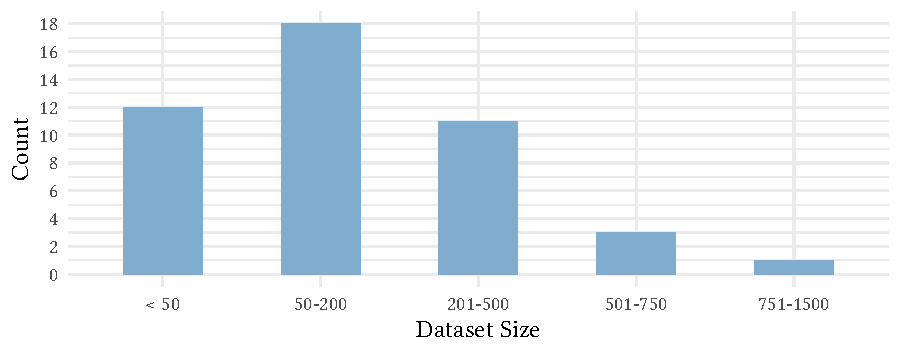
\includegraphics[width=\linewidth]{figures/survey/survey-dataset_size.pdf}
\caption[JPlag Survey: Dataset Size]{Results from the JPlag user survey~\cite{JPlagSurvey2024} regarding the question: \textit{What is your typical dataset size (number of programs)?}}
\label{fig:survey-dataset-size}
\end{figure}

\begin{figure}[p]
\centering
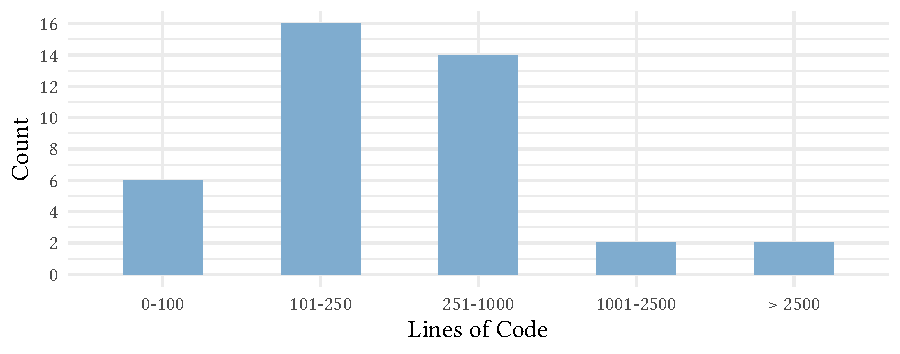
\includegraphics[width=\linewidth]{figures/survey/survey-program_size.pdf}
\caption[JPlag Survey: Program Size]{Results from the JPlag user survey~\cite{JPlagSurvey2024} regarding the question: \textit{What is the estimated average size of a single program (in lines of code)?}}
\label{fig:survey-program-size}
\end{figure}

\begin{figure}[p]
\centering
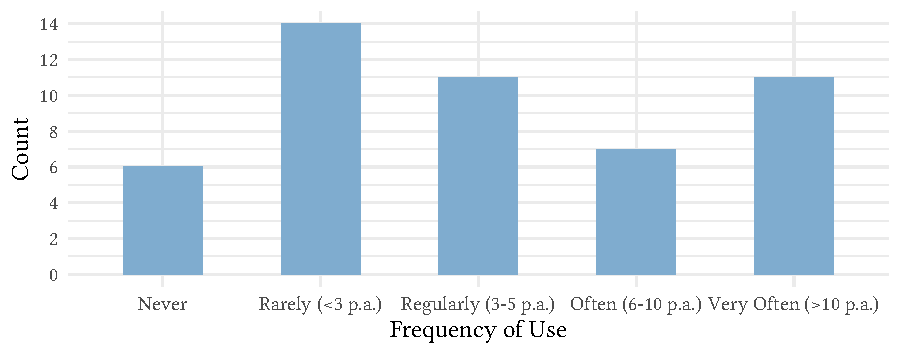
\includegraphics[width=\linewidth]{figures/survey/survey-frequency.pdf}
\caption[JPlag Survey: Usage Frequency]{Results from the JPlag user survey~\cite{JPlagSurvey2024} regarding the question: \textit{How frequently do you use JPlag?}}
\label{fig:survey-frequency}
\end{figure}

\subsection{Solution Space Problem}\label{sec:SPD-problem}
One of the primary challenges in plagiarism detection lies in the solution space. There are countless correct ways to implement a given solution in programming assignments. 
Thus, unrelated solutions by different students usually do not share many similarities. However, if the complexity of the assignments and hence the degree of freedom in the task is too low or the required solutions are small, the space of possible solutions decreases. Unrelated solutions become increasingly similar, and plagiarism detection becomes more challenging~\cite{Saglam2024b}.

At a certain point, the solution space collapses, strongly limiting the number of distinct solutions. It is no longer possible to differentiate plagiarism instances from accidental similarities between unrelated solutions. Thus, both manual and tool-based plagiarism will not produce any conclusive results and should not be considered.
An example of such an assignment would be writing a piece of code that prints the numbers from one to ten. While there are multiple ways to do it, there are not many. Thus, if students choose a similar or identical way, making assumptions about whether they plagiarize is impossible.

Let us consider a jigsaw puzzle as an analogy. While such a puzzle can be complex, there is only one valid solution. If multiple students now provide the same solutions for such a puzzle, we would not be surprised and would certainly not consider the possibility of plagiarism.
Now, let us consider the task of painting for a given motive; let us say a meadow with a single tree in the center. Here, many possible solutions, maybe even infinite solutions, exist. If now two students produce the same painting with the same colors and brushstrokes, we would be immediately suspicious, as the chance of that happening coincidentally is next to impossible.

This analogy holds true for programming assignments. A complex task requiring a large program to solve it is the counterpart to the painting. Here, plagiarism detection is very effective, and unrelated solutions are dissimilar. However, for trivial programming assignments, for example, used at the beginning of a course for novice programmers, plagiarism detection does not apply. Note that this is an inherent problem and exists both for human inspection and tool-based solutions.  

Educators must be conscious of these limitations. Therefore, plagiarism detectors should be designed to enable teachers to recognize situations where the results lack conclusiveness, enabling them to make well-informed and ethical decisions.

\section{Plagiarism Generators}
Plagiarism generators are programs that implement automated obfuscation attacks in order to generate plagiarism instances for a given input.
In the following, we discuss two algorithmic plagiarism generators~\cite{DevoreMcDonald2020, Broedel2023}. Moreover, we also discuss how generative AI, especially \acp{LLM}, can be exploited to serve as plagiarism generators.

\subsection{\mossad}\label{sec:foundations-mossad}
\textcite{DevoreMcDonald2020} introduce the so-called approach called \mossad\footnote{Capitalization chosen by the author of this dissertation to avoid any possible confusion between terms.}, a software plagiarism generator that rapidly produces obfuscated versions of original programs. Currently, \mossad is limited to C and C++ source code.
\mossad uses techniques inspired by genetic programming to evade plagiarism detection and randomly inserts statements until the similarity to the input computed by a plagiarism detector falls below a user-defined threshold. To keep the inserted statements domain-related and unsuspicious, \mossad uses both existing statements from the input program and a user-defined pool of statements called \textit{entropy}.
\mossad generates multiple variants from a single original, which are not only obfuscated from the original but also among each other due to its indeterministic nature.

During generation, \mossad randomly inserts statements from the pool into the variant.
Next, it checks if the variant still compiles and the semantics are preserved. If either one is not the case, the statement is not used.
After that, it uses a plagiarism detector, such as JPlag or MOSS, to compare the variant to the input program. If the similarity score is below the desired threshold, the corresponding variant is outputted as the final result. If not, this process is repeated.
%
To determine program semantic equivalence, \mossad compares the intermediate representation of programs after compiling both with high-level optimization. %This approach allows it to identify mutations that would be compiled away, such as dead code and redundant assignments.
%
By repeatedly applying mutations randomly, \mossad can create multiple variants that are different enough not to get flagged during plagiarism detection.
Its automatic and efficient nature makes it a potent threat to current plagiarism detection practices.

\mossad demonstrates its effectiveness
against various plagiarism detectors, including MOSS~\cite{MOSS}, Sherlock~\cite{Joy1999}, and JPlag~\cite{prechelt2000,prechelt2002}.
Their approach is mainly designed against token-based plagiarism detectors but has the potential for attacks on other structure-based~\cite{Nichols2019} software plagiarism detectors.

\subsection{PlagGen}
\textit{PlagGen} is a plagiarism generator introduced by \textcite{Broedel2023}.
Originally, it was called \textit{JPlag-Gen}, as it was used to evaluate JPlag. However, we refer to it as PlagGen for the remainder of this dissertation to avoid confusion. PlagGen is inspired by \mossad but has a few key differences. Instead of minimizing the similarity threshold of a target detector, it aims to insert statements at every possible position in the original source code. While it still employs random statements, it is less deterministic than \mossad. However, it avoids issues where some program parts are obfuscated while others are not.

While \mossad exclusively uses insertion~\cite{DevoreMcDonald2020},  PlagGen considers both insertion and reordering of statements.
PlagGen generates plagiarized programs using these two modes separately or in combination.
It first produces a plagiarized program using reordering and then applies insertion on the result, as reordering is considered a weaker attack \cite{Broedel2023}.

PlagGen is primarily designed for Java but could be implemented for other languages.
For insertion, PlagGen uses a similar approach to \mossad by inserting a random statement at a random position and using a compiler to check if the functionality remains unchanged. The key differences include using the Eclipse Compiler for Java (ECJ) instead of the GNU Compiler Collection (GCC), as ECJ can be configured to remove unused variables, thereby supporting most of the functionality of \mossad for Java.
For reordering, PlagGen identifies independent statements that can be swapped without affecting program functionality. It tests for independence based on indentation, control flow keywords, and variable accesses. This approach ensures that only valid modifications are made, thus preserving the program's behavior while effectively obfuscating the code.

While PlagGen is based on the insertion and reordering of statements, this attack can also be modified to employ other types of changes, for example, the automated application of refactoring transformations~\cite{Maisch2024}.


\subsection{Generative Artificial Intelligence}

The rapid development of generative AI, mainly via \acp{LLM}, has introduced new challenges in detecting and preventing plagiarism. AI-based attacks~\cite{Biderman2022}, which leverage these language models, present a growing concern for academic integrity in computer science education. Generative AI can now effectively function as a tool for plagiarism generation~\cite{Khalil_Er_2023}, with \acp{LLM} able to generate and modify code autonomously~\cite{Camara2023, Daun2023}.

Although \acp{LLM} have been critically described as \textit{Stochastic Parrots}~\cite{Bender2021}, they are criticized for lacking proper language understanding (although some researcher argues otherwise~\cite{Hinton2024}) and instead solely rely on statistical patterns.
However, this stochastic imitation is often sufficient to produce human-like code and text for plagiarism. While code generated by generative AI frequently contains flaws~\cite{Choudhuri2024, Camara2023, Ouyang2023}, these imperfections may work in favor of an adversary, as novice students' programs are rarely flawless, making AI-generated code appear realistic in educational settings.
\citet{Biderman2022} demonstrate that pre-trained language models can manipulate code to evade detection by MOSS~\cite{MOSS}, revealing vulnerabilities in current detection methods and emphasizing the need for more robust approaches

Compared to traditional plagiarism generators, generative AI is widely accessible to students. Tools like ChatGPT~\cite{ChatGPT} offer a simple, conversational interface, democratizing access to generative AI and accelerating its adoption~\cite{Saglam2024a}. This \textit{commodification} of generative AI has significantly lowered the barrier for automated obfuscation, making it easier than ever for students to mask plagiarized code, further exacerbating the challenge for educators and detection systems~\cite{ChatGPTGuide}.

For cheating in programming assignments, generative AI can serve two primary purposes in facilitating plagiarism: generating code from scratch and obfuscating existing solutions~\cite{Saglam2024a, Saglam2024b}.
%
The first scenario, \textit{full solution generation}, uses \acp{LLM} to create a solution from scratch based on an assignment description as a prompt. Here, there is an ongoing debate on whether this form of cheating qualifies as plagiarism~\cite{Novak2019, Saglam2024a}.
%
The second scenario, \textit{automatic obfuscation}, involves using generative AI to alter an existing solution's structure without altering its functionality, effectively concealing its origin. This closely resembles human obfuscation practices~\cite{Novak2019}.

Although generated solutions may exhibit higher similarity due to \acp{LLM} semi-deterministic nature, detecting them with low false positives is challenging.
However, current research suggests that automatic obfuscation may be the more effective approach for medium to large assignments, as \acp{LLM} struggle to generate reliable solutions for complex tasks~\cite{Choudhuri2024, Saglam2024b}.
Nevertheless, entirely generated solutions are increasingly feasible for smaller programs, although the effectiveness of these approaches continues to be a topic of research~\cite{Qadir2023}.

\section{Model-Driven Engineering}

Modeling is essential in software development and other fields~\cite{Stahl2006}. It allows designers and engineers to explore design options efficiently, offering stakeholders clear representations of the system being studied. Models enable all participants to understand, analyze, and design complex software and other systems~\cite{Kienzle2024}.

According to the definition by \citet{Stachowiak1973}, a model possesses three fundamental properties: First, it serves as a \textit{mapping} of the archetype it represents. Second, it functions as an abstraction or \textit{reduction} of this archetype, which means not every detail is described. Third, it embodies \textit{pragmatism}, as it is created for a specific purpose.

Model-driven engineering is an approach based on software engineering that considers models as first-class citizens of the development process~\cite{Brambilla2017}. This means that in \ac{MDE}, domain models are primary artifacts alongside code~\cite{Kent2002}.
\cite{Martinez2020} characterizes models as structured data defined by the metamodels they conform to, consisting of model elements that contain attributes and references. These basic building blocks allow for the construction of additional models. 

Metamodels thus describe a set of models, and each model is an instance of its metamodel. Therefore, metamodels exist one \textit{metalevel} above the models they describe~\cite{Stahl2006}.
According to \cite{Bezevin2005}, all \ac{MDE} artifacts, such as model transformations and model queries, can be represented as models themselves, allowing for a uniform treatment of these elements.

The structure of a model typically describes the specifics of the relationships between its elements. In this context, \textit{containment relations}, as recognized in \ac{UML}, indicate stronger relationships that express ownership among model elements.
While models and metamodels are often represented as tree-based structures formed by model elements and their relationships, it is essential to note that this is not universally the case.

To further distinguish between program code and modeling artifacts, it is useful to consider that code typically adheres to executable instructions intended for machine interpretation, while modeling artifacts, which are often domain models, serve as higher-level abstractions aimed at expressing logic or domain-specific structures. While there are executable models~\cite{Seidewitz2014, Fuksa2024}, not all models have well-defined dynamic semantics~\cite{Stahl2006}.

\subsection{Modeling Education}
Modeling is taught in software engineering courses, as modeling languages like \ac{UML} are widely used in practice~\cite{Engels2006, Stahl2006}.
Furthermore, modeling becomes more common in computer science education with the increasing adoption~\cite{Brambilla2017, Hutchinson2011} of model-driven techniques.
Consequently, computer science assignments and exams often include modeling assignments~\cite{Ciccozzi2018, Stahl2006, Saglam2023}, for example, \ac{UML} assignments regarding class, use case, sequence, and activity models.
%
Modeling education includes two aspects~\cite{Kienzle2024}: First, using modeling concepts, languages, and tools. This is more in line with modeling in fundamental software engineering courses. Second, modeling language engineering, metamodeling, and other model-driven concepts.

According to \cite{Ciccozzi2018}, most \ac{MDE} courses are offered at the master's level, leveraging students' prior knowledge in software engineering and modeling. However, some courses are also provided for bachelor's and PhD students. Typically, these courses combine lectures with labs to balance theory and hands-on practice, with many classes having over 90 students.
%
Typical \ac{MDE} courses mainly fall into two categories: domain-specific \ac{MDE} applications using established tools and courses that teach how to develop domain-specific \ac{MDE} tools. These courses cover core concepts and techniques in \ac{MDE}, including language engineering and model transformation. Lectures often focus on meta-modeling to define abstract and concrete syntax and model transformation for code generation. Lab activities allow students to practice with common \ac{MDE} tools like the \ac{EMF}.

While most academic and industrial \ac{MDE} tools are not ideal for teaching modeling~\cite{Kienzle2024}, many education-specific tools exist. In the following, we give some examples of tools for \ac{MDE} education.
%
\textit{Umple}~\cite{Lethbridge21} is an open-source modeling tool that combines graphical and textual interfaces to help students design class diagrams, state machines, and feature models.
\textit{TouchCORE}~\cite{ali2022} is an academic modeling tool centered on reusing and customizing domain-specific languages to enhance students' understanding of complex modeling tasks.
The \textit{Epsilon Playground}~\cite{KolovosGarciaDominguez22} provides web-based examples that allow students to practice with modeling languages directly in the browser, removing the need for complex installations.
The \textit{MDENet} education platform~\cite{Barnett2023} offers a customizable environment where different \ac{MDE} tools can be integrated, allowing educators to create and share interactive modeling activities directly accessible to students online.
\textit{AToMPM}~\cite{Syriani2013b} is a web-based graphical modeling environment that lets students define domain-specific modeling languages with a fully customizable editor.
The \textit{ENCORE} platform~\cite{ENCORE-MODELS23} supports educators in designing personalized learning paths in \ac{MDE} by integrating open educational resources.

\subsection{Modeling Plagiarism Detection}

Modeling assignments are prone to plagiarism due to their complexity and their requirement of domain understanding and problem-solving skills~\cite{Martinez2020}.
However, there is little research on modeling plagiarism and its detection \cite{Martinez2020, Saglam2022, Saglam2023}.
While automated plagiarism detection was proposed decades ago \cite{Ottenstein1976, prechelt2000}, most state-of-the-art plagiarism detectors can only be used with code~\cite{Novak2020}.

While model differencing~\cite{Stephan2013, Kolovos2009} and model clone detection~\cite{Stoerrle2015, Babur2019, Shobha2021} are well researched, these techniques alone are insufficient for plagiarism detection, as they are not resilient against obfuscation attempts~\cite{Wittler2023, Saglam2022, Martinez2020}.
This is unsurprising, as both techniques are not intended for an attacker-defender scenario, e.g., where an attacker purposefully attempts to obfuscate modeling clones or prevent model differencing from correctly deriving the differences between models.

To the author's knowledge, there is only one other approach for modeling plagiarism detection.
\citet{Martinez2020} utilize \emph{Locality Sensitive Hashing} (LSH), an approximate nearest neighbor search mechanism, to detect plagiarism. They embed models into a similarity metric space by transforming them into context-aware fragments that are turned into integer vectors using \textit{minhash} on the names of the fragment's classes, attributes, and operations.
Context-aware fragments are essentially smaller components of the model, which are analyzed in their context, meaning the relationships and properties are considered.
The model signatures are then computed based on these vectors using LSH, and the similarity of any two models is determined by the hamming distance between the two signatures~\cite{Martinez2022}. 

As this approach relies on LSH, it involves several hyperparameters that require adjustment to optimize detection rates for modeling domains. Key parameters include the number of bands, which determines the strictness of signature matching by providing independent opportunities for items to match, and the number of rows per band, which balances precision and recall by adjusting the required signature length for similarity. A higher number of bands with fewer rows increases selectivity, while fewer bands with more rows relax the criteria, identifying more candidate pairs. Proper tuning of these parameters is essential for maximizing the approach's effectiveness~\cite{Martinez2020}.

While this approach effectively detects plagiarism, it combines contextual rather than structural information, making it vulnerable to \textit{some} obfuscation attacks.
The LSH signatures are computed based on names, so their approach is prone to renaming-based obfuscation attacks.
Moreover, this approach does not provide typical traceability features that common approaches for source code plagiarism provide.
This means that, given a similarity score between two models, there is no information about which parts of the models were matched and which parts differed.

\part{Contributions}
\chapter{Threat Model}\label{cha:threatmodel}

\noindent
\textit{Obfuscation attacks} aim to avoid detection by strategically altering a plagiarized program, thus obscuring the relation to its original~\cite{Saglam2024b}.
As state-of-the-art detection approaches compare the structure of programs by identifying similarities between code fragments~\cite{Nichols2019}, obfuscation attacks try to alter the structural properties of the program, ideally without affecting its behavior~\cite{Novak2020, Karnalim2016, Pawelczak2018}.
The intended outcome is to disrupt the matching of fragments between programs (as seen in \autoref{tab:re-tokens}), thus leading to a reduced similarity score~\cite{DevoreMcDonald2020}.
Specifically, the goal is to prevent the detector from matching fragments above the specified match length cut-off threshold.
However, to impact the detection quality of a software plagiarism detector, the obfuscation must affect the linearized program representation of the detector, which in the case of token-based approaches is the token sequence~\cite{Saglam2024b}. Consequentially, modifications to the program code that do not affect the token sequence are inherently ineffective. For example, renaming elements like classes or members does not affect token-based approaches, as names are omitted during the tokenization~\cite{prechelt2000, Saglam2024a}.

To provide an understanding of the threat posed by automated obfuscation of plagiarism, we introduce a comprehensive threat model regarding obfuscation attacks targeting token-based software plagiarism detectors (\contribution{1}). This threat model highlights the danger of automated obfuscation attacks.
%
We focus on token-based approaches, as they are the de facto standard in practice. However, this threat model can be applied to other structure-based approaches, such as graph-based ones.

In the following, we first discuss an example of an obfuscation attack.
Second, we analyze the attack surface of token-based software plagiarism detection systems. We show that all obfuscation attacks must affect the internal program representation to disrupt the detection process.
Third, we provide a formal definition for key concepts.
Next, we categorize and relate different attack types regarding their effectiveness and applicability.
After that, we discuss the automation of obfuscation attacks via both algorithmic approaches and large language models.
Finally, we introduce the concept of \textit{intrusiveness}, which defines how much the program behavior is affected by obfuscation attempts.

\ownpublications{
\fancycite{Saglam2024b},
\fancycite{Saglam2024a},\\
and \fancycite{Saglam2024d}.
}

\section{Exemplary Obfuscation Attack}\label{sec:threatmodel-example}\label{sec:ase:RunningExample}

\noindent
We utilize the two programs depicted in \autoref{tab:running-example} as our illustrative example.
Both programs print the concatenated natural numbers from 1 to a specified maximum value. 
Notably, the variant on the right is a modified revision of the original on the left, produced via two structural changes that avoid altering the behavior of the program.
Specifically, a new variable named \texttt{debug} is inserted, and the array-style loop is replaced with a for-each loop.
Although the similarities between the two programs remain apparent for such a small example, this may not hold true when applying similar changes at a large scale.
Crucially, such alterations reduce the likelihood of detection by a plagiarism detector.

\autoref{tab:re-tokens} illustrates the internal, linearized representations of both programs. For simplicity, only the representations of the method bodies (lines 2-7) are depicted (signatures are omitted).
%These so-called token sequences contain only structural elements.
State-of-the-art plagiarism detectors linearize the programs by parsing them and extracting a subset of the parse tree nodes as \textit{tokens}~\cite{Saglam2024b}.
The resulting \textit{token sequences} consist solely of structural elements~\cite{prechelt2000}.
Details like names, types, values, and formatting are omitted, thus providing some obfuscation resilience.
Due to the modifications made to generate the variant, the token sequences of both programs are not identical.
As discussed in \autoref{sec:TPD}, all token-based software plagiarism detectors operate based on identifying common subsequences.
We can identify three matching subsequences (highlighted in grey), with each neighboring match interrupted by a single token.
Note that the differing tokens interrupt the matching. This includes a token on one side combined with the absence of one on the other and two tokens of different types on both sides.

In the example in \autoref{tab:re-tokens}, we use a cut-off threshold of two, meaning the minimum length of a match is two tokens. Matches below that length would be omitted. This value is solely chosen for illustrative purposes. In reality, the threshold would be higher. JPlag, for example, uses a default cut-off threshold of \textit{nine} tokens for Java programs and 12 tokens for C++ and Python programs. For most approaches, this threshold can also be adapted to a custom value by the user if desired.

%\todoTimur{Show that JPlag is resilient against retyping; maybe also rename a variable to show resilience against lexical changes?}

\begin{samepage}
\begin{table}[p]
	\centering
	\begin{tabular}{rlcl}
		\toprule
		\textbf{\#} & \textbf{Original}                                  &                                    & \textbf{Variant}                                \\
		\midrule
		1           & \texttt{printNumbers(int max) \{}                  &                                    & \texttt{printNumbers(int max) \{}               \\
		2           & \texttt{~~int[] n = range(0,max);}                 &                                    & \texttt{~~int[] n = range(0,max);}              \\
		3           & \texttt{~~String result = "";}                     &                                    & \texttt{~~String result = "";}                  \\
		        
		4           &                                                    & \textbf{\phantom{$\to$}  insert $\to$} & \cellcolor{add}\texttt{~~int debug = n.length;} \\
				
		5           & \cellcolor{del}\texttt{~~for(int i=0; i<max; i++)} & \textbf{$\to$ alter $\to$}   & \cellcolor{add} \texttt{~~for(int number : n)}  \\
		6           & \cellcolor{del}\texttt{~~~~result += n[i];}        & \textbf{$\to$ alter $\to$}   & \cellcolor{add} \texttt{~~~~result += number;}                  \\
		7           & \texttt{~~println(result);}                        &                                    & \texttt{~~println(result);}                     \\
		8           & \texttt{\}}                                        &                                    & \texttt{\}}                                     \\
		\bottomrule
	\end{tabular}
    \caption[Example Obfuscation: Insertion and Alteration]{Original and obfuscated programs illustrating obfuscation techniques. The original code is displayed on the left, and the obfuscated variant is on the right. The modifications include inserting a new statement in line 4, altering the loop type in line 5, and modifying a loop body statement in line 6. Removed lines are highlighted in red, and added lines are highlighted in green.}%{Original code (left) and modified variant (right) after inserting one statement and altering one. Removed lines are highlighted in red, and added lines are highlighted in green.}
	\label{tab:running-example}
\end{table}


\begin{table}[p]
	\centering
	\begin{tabular}{c
 c c cc}
		\toprule
		type & \textbf{Original Tokens} &                            & type & \textbf{Variant Tokens} \\
		\midrule
		\match 
		1  & \texttt{variable}        &                            & 1  & \texttt{variable}       \\
		\match 
		2  & \texttt{apply}           &                            & 2  & \texttt{apply}          \\
		\match 
		1  & \texttt{variable}        &                            & 1  & \texttt{variable}       \\
           &                          & \phantom{$\to$} \textbf{insert} $\to$               & \cellcolor{add}1  & \cellcolor{add}\texttt{variable}       \\
		\match 
		3  & \texttt{loop start}      &                            & 3  & \texttt{loop start}     \\
		\match 
		1  & \texttt{variable}        &                            & 1  & \texttt{variable}       \\
						         
		\cellcolor{del}4  & \cellcolor{del}\texttt{assign}          & $\to$ \textbf{remove} \phantom{$\to$} &    & \texttt{}               \\
		\match 
		4  & \texttt{assign}          &                            & 4  & \texttt{assign}         \\
		\match 
		5  & \texttt{loop end}        &                            & 5  & \texttt{loop end}       \\
		\match 
		2  & \texttt{apply}           &                            & 2  & \texttt{apply}          \\
		\bottomrule
	\end{tabular}
    \caption[Example Obfuscation Tokens: Insertion and Alteration]{Original and obfuscated token sequences corresponding to the method bodies of the programs in \autoref{tab:running-example} with three matching subsequences highlighted in gray (in detail these are $(1, 2, 1)$, $(3, 1)$, and $(4, 5, 2)$). They are interrupted by two differences in the token sequence: the insertion of a token highlighted in green, and the removal of a token highlighted in red.}
	\label{tab:re-tokens}
\end{table}

\end{samepage}
        
\section{Attack Surface Analysis}\label{sec:threatmodel-analysis}
%\todo{Examination of the attack surface of token-based plagiarism detection systems from the perspective of obfuscation attacks. Identify the entry points and vulnerabilities adversaries exploit to alter token sequences and evade detection.}

Obfuscation attacks affect the detection quality during the pairwise comparison by splitting up subsequences until they fall under the matching threshold of the detector and are thus omitted.
As token-based detectors solely use the internal representation of the programs for subsequence matching, the token-sequence, being that representation, is the only attack surface.

Consequentially, for \textit{any} obfuscation attack to be effective, it needs to affect the token sequence. Moreover, to interrupt the subsequence matching enough to reduce the calculated similarity, the attack must broadly affect the token sequence, meaning consistently over the entire sequence length. To provide an inverse example, if only the first quarter of a token sequence is altered, the matching will be disrupted only for that part. As a result, the similarity can never drop below 75 percent since that percentage of the token sequence remains matched.
Note that while the token sequence is the attack surface, it cannot be directly altered. Instead, the program code needs to be altered to lead to a different token sequence. For this reason, simple techniques like renaming have no effect on token-based approaches. While they change the program, names are not considered during the tokenization and thus do not affect the token sequence (see \autoref{sec:TPD}).

\autoref{tab:re-tokens} illustrates how the effect of the obfuscation attempts in \autoref{tab:running-example} affect the subsequence sequence matching. While only two tokens are affected, the matching is disrupted, and only three subsequences are matched. For a hypothetical cut-off threshold of four tokens, all three would be ignored, thus reducing the similarity from 100\% to 0\%. 
Note how renaming variables in the original programs would not affect the internal representation of the derived token sequences, as this type of information is not present.

As each token only encapsulates its type, meaning what kind of program element, such as control structures or variable definitions, it represents, the token sequence can be seen as a sequence of integers. \autoref{tab:re-tokens} shows this integer representation but also the type itself (e.g., apply or variable).
Based on this, there are inherently two possible atomic types of alterations: Deleting a token from the sequence and inserting a token into the sequence. We also consider changing the position of a token in the sequence as an essential alteration. However, it is technically not atomic, as it is equal to one deletion and one insertion. Note that a formal definition will follow in the subsequent section.

\begin{figure}[hb]
    \centering
    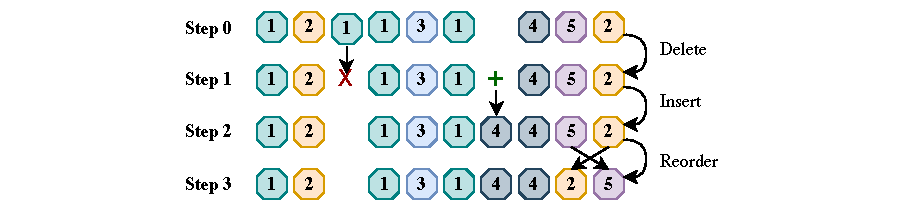
\includegraphics[width=\linewidth]{figures/atomic.pdf}
    \caption[Atomic Changes on Token Sequence Level]{Stepwise combination of three atomic modifications (token deletion, insertion, and reordering) for a token sequence. Any effective obfuscation attack must affect the token sequence.}
    \label{fig:sequence-modification}
\end{figure}

\autoref{fig:sequence-modification} illustrates these three types of alterations on example sequences.
The effects of all possible obfuscation attacks, no matter how simple or complex, can be broken down into a combination of these atomic changes.
Note that while these modifications may stem from obfuscation attacks, they can also arise when computing the difference between two unrelated programs.
Thus, the presence of certain types of changes between two token sequences alone cannot provide any indication of plagiarism.

\section{Formal Definition of Token Sequence Modification}\label{sec:threatmodel-algebra}

For plagiarism detection purposes, a linearized program can be seen as a token sequence \((a_i)_{i=1}^{l}\), where each token \(a_i\) represents a structural element of a program.
For the similarity calculation, a plagiarism detector only requires information on whether two tokens represent the same type of program element and should, therefore, be considered equivalent. 
Thus, a token sequence, in its essence, can be represented as a finite sequence of natural numbers, where each number represents a specific type of program element.

\begin{theorem}[Token Sequence]
    A token sequence \((a_i)\) is a finite sequence \((a_i)_{i=1}^{l}\) of tokens \( a_i \in \mathbb{N}\) where \(i \in \mathbb{N}\) denotes the index of a token and \(l \in \mathbb{N}\) denotes the length of the token sequence.
\end{theorem}

\begin{theorem}[Token Sequence Set]
    We define the set of all token sequences as \(\mathbf{S}\).
\end{theorem}

Plagiarism detectors compute subsequence matches to compare two token sequences and assess their similarity.
A match between two token sequences \((a_i)\) and \((b_j)\) is defined as a shared subsequence, which means it is itself a sequence that appears in both given sequences.

\begin{theorem}[Subsequence]
    Consider two token sequences \((a_i)_{i=1}^l\) and \((b_j)_{j=1}^n\). \((b_j)\) is a \textit{subsequence} of \((a_i)\), denoted by the relation
    \begin{align*}
         (b_j) \sqsubseteq (a_i)
    \end{align*}
    if 
    \begin{align*}
         \exists \, d \in \mathbb{Z} \quad \text{such that} \quad \forall j \in \{1, 2, \ldots, n\} \quad b_j = a_{j+d}.
    \end{align*}
\end{theorem}

\begin{theorem}[Subsequence Match]\label{def:subsequence-match}
    Let \((a_i)_{i=1}^l\), \((b_j)_{j=1}^n\) and \((m_k)_{k=1}^o\) be token sequences.
    Then \((m_k)\) is a subsequence match of \((a_i)\) and \((b_j)\) if
    \begin{align*}
        (m_k) \sqsubseteq (a_i) \: \land \: (m_k) \sqsubseteq (b_j).
    \end{align*}
\end{theorem}

We thus define the number of matching tokens between two token sequences as the sum of the lengths of all disjoint (non-overlapping) matching subsequences shared by the two sequences.

\begin{theorem}[Matching Tokens]\label{def:matching-tokens}
    Let \((a_i)_{i=1}^l\), \((b_j)_{j=1}^n\), and \((m_k)_{k=1}^o\) be token sequences and let \(M\) be the set of all disjoint subsequence matches for \((a_i)\) and \((b_j)\).
    We then define the number of matching tokens \(m((a_i), (b_j))\) as
    \begin{align*}
        m : \mathbf{S} \times \mathbf{S} \rightarrow \mathbb{N}
    \end{align*}
    with
    \begin{align*}
        m((a_i), (b_j)) = \sum_{(m_k) \in M}|(m_k)|
    \end{align*}
    where \(|(m_k)|\) is the length \(o\) of the token sequence \((m_k)\). Note that \(m((a_i), (b_j)) \leq l, n\).
\end{theorem} 

Since two token sequences can share multiple disjoint non-overlapping subsequences, \(m((a_i), (b_j))\) aggregates the length of all such disjoint matching subsequences. In practice, plagiarism detectors do not try to find the set of such disjoint subsequent that maximize \(m((a_i), (b_j))\); rather, they employ a greedy approach in order to find a suitable subsequence matching efficiently~\cite{Wise1993}.

The similarity of a token sequence \((a_i)\) to another sequence \((b_j)\) can be defined as the ratio of the number of matching tokens (usually based on a set of matches) to the length of the first sequence.

\begin{theorem}[Asymmetric Similarity] \label{theo:similarity}
    Let \((a_i)_{i=1}^l\), \((b_j)_{j=1}^n\) be token sequences.
    We then define similarity of \((a_i)\) to \((b_j)\) as
    \begin{align*}
    \operatorname{sim} : \mathbf{S} \times \mathbf{S} \rightarrow \mathbb{Q}
    \end{align*}
    with
    \begin{align*}
        \operatorname{sim}((a_i), (b_j)) = 
        \begin{cases}
            \frac{m((a_i), (b_j))}{l}, & \text{if } l > 0\\
            0, & \text{otherwise} .
        \end{cases}
    \end{align*}
\end{theorem}

The similarity metric \(sim\). defined in \autoref{theo:similarity} describes the proportion of tokens in sequence \((a_i)\) that are matched to tokens in sequence \((b_j)\).

It is important to note that the lengths of the token sequences \((a_i)\) and \((b_j)\) can differ.
The similarity \( {sim}_{(a_i) \rightarrow (b_j)} \) is thus not symmetric, meaning \( {sim}_{(a_i) \rightarrow (b_j)} \) is not necessarily equal to \( {sim}_{(b_j) \rightarrow (a_i)} \). However, it is used as it allows one to reason about how much of one program is matching another and vice versa.
To measure the overall similarity between two sequences, we often use symmetric metrics such as maximum similarity and symmetric similarity.

\begin{theorem}[Symmetric Similarity] \label{theo:avgsim}
    Let \((a_i)_{i=1}^l\), \((b_j)_{j=1}^n\) be token sequences.
    We then define the symmetric similarity as
    \begin{align*}
    \operatorname{symsim} : \mathbf{S} \times \mathbf{S} \rightarrow \mathbb{Q}
    \end{align*}
    with
    \begin{align*}
        \operatorname{symsim}((a_i), (b_j)) = \frac{2 \, m((a_i), (b_j))}{l+n}
    \end{align*}
\end{theorem}

\begin{theorem}[Maximum Similarity] \label{theo:maxsim}
    Let \((a_i)_{i=1}^l\), \((b_j)_{j=1}^n\) be token sequences.
    We then define the maximum similarity as
    \begin{align*}
    \operatorname{maxsim} : \mathbf{S} \times \mathbf{S} \rightarrow \mathbb{Q}
    \end{align*}
    with
    \begin{align*} 
     \operatorname{maxsim}((a_i), (b_j)) = \max(\operatorname{sim}((a_i), (b_j)),\, \operatorname{sim}((b_j), (a_i)))
\end{align*}

\end{theorem}

These metrics defined \autoref{theo:avgsim} and \autoref{theo:maxsim} provide a more comprehensive view of the similarity by considering both directions in a pairwise comparison of programs.
For simplicity, we use the term \textit{similarity} referring to the symmetric similarity throughout the remainder of this dissertation unless specified otherwise.

Finally, regarding obfuscation attacks, we previously established that they all result in a combination of fine-grained modifications of token sequences. To understand how token sequences can be modified, consider the following possible \textit{atomic} modifications:

\begin{theorem}[Token Insertion]
    Inserting a token \(t \in \mathbb{N}\) into a given token sequence \((a_i)_{i=1}^l\) at index \(k \in \mathbb{N}, k < l\) is defined as
    \begin{align*}
            \operatorname{ins} : \mathbb{N} \times \mathbf{S} \times \mathbb{N} \rightarrow \mathbf{S}
    \end{align*}
    with
    \begin{align*}
        \operatorname{ins}(t, (a_i), k) = (a_1, \dots, a_{k-1}, t, a_k, \dots, a_l)
    \end{align*}
\end{theorem}

\begin{theorem}[Token Deletion]
     Deleting a token at index \(k \in \mathbb{N},\, k < l\) in a give token sequence \((a_i)_{i=1}^l\) is defined as
    \begin{align*}
            \operatorname{del} : \mathbf{S} \times \mathbb{N} \rightarrow \mathbf{S}
    \end{align*}
    with
    \begin{align*}
        \operatorname{del}((a_i), k) = (a_1, \dots, a_{k-1}, a_{k+1}, \dots, a_l)
    \end{align*}
\end{theorem}

We also consider the following non-atomic operations as essential:

\begin{theorem}[Token Swapping]
     Swapping two tokens can be defined based on the combined insertion and deletion of two tokens,
     Given a token sequence \((a_i)_{i=1}^l\) and two indices \(k_1, k_2 \in \mathbb{N},\, k_1, k_2 \leq l \) we thus we define it as
    \begin{align*}
            \operatorname{swap} : \mathbf{S} \times \mathbb{N} \times \mathbb{N} \rightarrow \mathbf{S}
    \end{align*}
    with
    \begin{align*}
        \operatorname{swap}((a_i), k_1, k_2) = {ins}(a_{k_2}, {ins}(a_{k_1}, {del}({del}((a_i), k_1), k_2 - 1), k_2), k_1)
    \end{align*}
\end{theorem}

\begin{theorem}[Token Reordering]
    Let \((a_i)_{i=1}^l\) be a token sequence, \(\mathbf{S}_l\) be the set of all token sequences of length \(l\), and \(\mathbf{G}_l\) the set of all permutations in \(\mathbf{S}_l\)
   % Let \(\mathbf{S}_l\) be the set of all token sequences of length \(l\), and let \(\mathbf{G}_l\) be the set of all permutations
    \begin{align*}
        \sigma_l : \{1, 2, \dots, l\} \to \{1, 2, \dots, l\} \,.
    \end{align*}
    We define the reordering of tokens for sequences of length \(l\) as
    \begin{align*}
        \operatorname{reorder}_l : \mathbf{S}_l \times \mathbf{G}_l \rightarrow \mathbf{S}_l
    \end{align*}
    with
    \begin{align*}
        \operatorname{reorder}_l((a_i), \sigma) = (a_{\sigma_l(1)}, a_{\sigma_l(2)}, \dots, a_{\sigma_l(l)}) \,.
    \end{align*}
    The general reordering function is then defined as the combination of \(\operatorname{reorder}_l\) for all \(l \in \mathbb{N}\).
\end{theorem}

An obfuscation attack on a token sequence is thus defined as a set of changes to an input program that cause a series of atomic modifications to the token sequence derived from that program. The aim of such an attack is to lower the similarity of the modified token sequence to the original token sequence. Specifically, if a token sequence \((a_i)\) is a copy of another token sequence \((b_j)\), an obfuscation attack on \((a_i)\) modifies it such that the similarity falls below a threshold \(L \in \mathbb{Q}\).
Here, \(L\) is the target similarity threshold below which the similarity is deemed suspicious. Note that choosing a suitable \(L\) is up to the adversary.

\section{Categorization of Obfuscation Attacks}\label{sec:threatmodel-categorization}
The challenge for an adversary lies in finding the optimal combination of changes that maximize obfuscation\footnote{In a simplified framework, obfuscation could be seen as the opposite of similarity, e.g., along the lines of $obf_{(a_i) \rightarrow (b_j)} = 1- sim_{(a_i) \rightarrow (b_j)}$. However, not every obfuscation attempt and not every modification done as part of such an attempt is effective, which is why this relationship cannot be described so trivially.
} while minimizing the impact on the original behavior of the program.
We classify potential obfuscation attacks on a conceptual scale from verbatim copying, which is the absence of any obfuscation, to semantic clones, which are inherently hard to detect, as they have to be distinguished from unrelated, similar programs by students who did not plagiarize. Note that this scale stems from the clone type levels of \citet{Faidhi1987, Karnalim2016}. While clone detection scenarios lack the complexity of the adversarial aspects of plagiarism detection, similarities can be drawn between clone types and obfuscation types.

\autoref{fig:clone-types} illustrates this conceptual scale.
We define the following categories:
\begin{description}
    \item[Lexical Attacks] include renaming elements, changing comments, altering the code formatting, whitespace manipulation, and symbol substitution (e.g., parentheses and brackets).
    \item[Data-Based Attacks] cover type changing data types, replacing literals with equivalent but differently represented values, and adjusting the precision of numeric values.
    \item[Structural Attacks] involve fine-grained changes to the program structure, such as dead code insertion and the reordering of independent statements.
    \item[Complex Attacks] include refactoring-based attacks like changing loop types, code (de-) fragmentation, inheritance hierarchy manipulation, and modifying the control flow structure. 
    \item[Re-implementation] includes both partial re-implementation, for example, replacing a sorting algorithm with another one, as well as full implementation, which produces semantic clones.
\end{description}
Returning to our example in \autoref{tab:running-example}, statement insertion is a structural attack, while loop modification exemplifies a complex attack, albeit a simple instance.

We make no strong assumptions about the type of programming language in this categorization. While some categories or specific obfuscation attacks of a category only apply to imperative languages such as Java or C++, others apply to any given programming language.
%
Lexical Attacks apply to most languages, including functional ones.
Data-based attacks can be adapted to functional languages by manipulating data representations.
Structural Attacks, which rely on modifying the code's structure, can also be applied to functional constructs, though the way control flow is structured might differ.
Complex Attacks apply to any language, but the methods may be language-specific (e.g., recursion-heavy control flow in functional languages vs. loops in imperative ones).
Re-implementation is a concept applicable across languages.
%
Consequentially, for functional languages like Haskell, only some obfuscation attacks are valid threats. However, this means the attack space is less diverse than that of other languages. Moreover, differences in language constructs may influence the implementation of specific obfuscation techniques.
Thus, our categorization can be adapted and applied to various programming paradigms. Nevertheless, this dissertation focuses mainly on imperative languages or languages that at least support imperative constructs (e.g., Scala, F\#).
%
Consequently, no strong language-specific assumptions limit this categorization of obfuscation attacks.

Note that the categories in \autoref{fig:clone-types} are not exhaustive and may overlap in rare cases, as some obfuscation attacks may manifest in multiple categories depending on their specific implementation. Instead, they showcase different manifestations of obfuscation attacks~\cite{Novak2019, Karnalim2016}. As discussed, the attack surface for \textit{all} of these attacks remains the actual token sequence and how it affects the subsequence matching.
Moreover, as noted in the attack surface analysis, we cannot make assumptions about the presence of plagiarism or obfuscation based on the aforementioned categories alone. For example, statement insertion can be part of an obfuscation attempt, but it can also just be the difference between two unrelated solutions, where one contains these statements, such as additional debug output, while the other does not.

Token-based approaches are inherently resilient to \textit{lexical} obfuscation attacks~\cite{Joy1999}, but an adversary may nevertheless employ them to alter the appearance of the program to the human eye\footnote{To the best of our knowledge, there are no established metrics to define such a property. Also, note that this type of obfuscation is outside the scope of this dissertation, as we focus on obfuscation attacks that target software plagiarism detectors to affect their computed similarity scores.}.
Provided they employ proper tokenization, most approaches are also resilient against data-based attacks.
For instance, changing the name or value of the inserted debug statement in \autoref{tab:running-example} would not impact the derived tokens in \autoref{tab:re-tokens}.
\autoref{fig:clone-types} also illustrates the effect strength of these attack types. With rising complexity, the effect of the token sequence grows larger.
However, with rising complexity, the applicability becomes less broad. For example, dead code insertion can be applied almost everywhere in a code base, while specific refactoring attacks can only be executed where the refactoring preconditions are met~\cite{Saglam2024b}.

        \begin{figure}
            \centering
            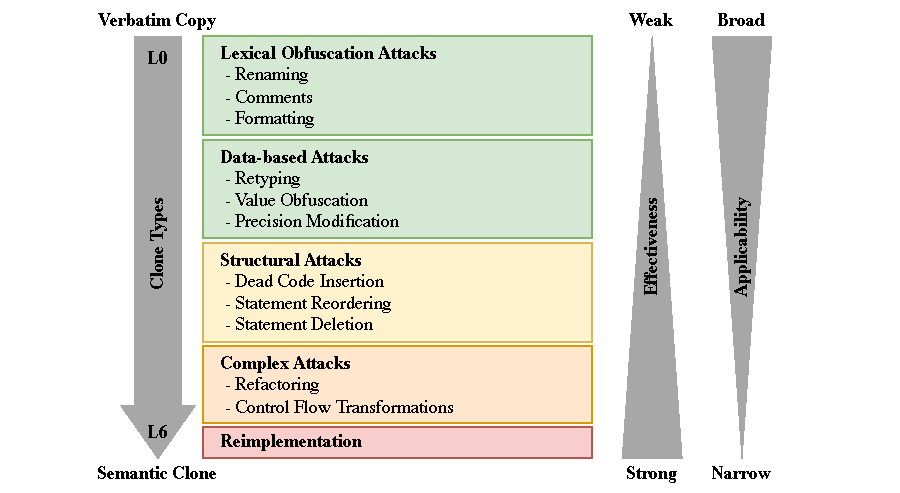
\includegraphics[width=\linewidth]{figures/threatmodel/Classification.pdf}
            \caption[Categorization of Obfuscation Attack Types]{Categorization of obfuscation attacks corresponding to the clone types by \citet{Karnalim2016, Faidhi1987}, thus illustrating the effect of the attacks on the token sequence as well as how broadly they can be applied.}
            \label{fig:clone-types}
        \end{figure}

An important limitation of our threat model concerns semantic clones. Once a certain level of re-implementation is reached, the program code may look distinct but behave identically\footnote{There is ongoing debate about what defines the behavior of a program in the context of plagiarism detection. Even fundamental questions remain contested, such as whether print statements should be considered debugging output or part of the intended behavior of a program. In practice, it depends on the educational context at hand. Methods and tools must be adapted or configured for institutions or individual courses.}. The challenge lies in accurately distinguishing these cases without erroneously flagging unrelated programs as false positives. It is worth noting that this limitation is intrinsic to plagiarism detection, whether conducted by humans or through automated tools.
Interestingly, adversaries face a similar challenge in determining the optimal extent of changes required to avoid detection while maximizing the grade or points earned and minimizing effort.
        
\section{Automation of Obfuscation Attacks}\label{sec:threatmodel-automation}
As discussed previously, automated obfuscation attacks refute the established assumption that evading detection requires more effort than completing the actual assignment~\cite{Joy1999, DevoreMcDonald2020}.
While designing such an automated attack is complicated, using it is not.

A notable example of such automated attacks is \mossad~\cite{DevoreMcDonald2020}, which repeatedly inserts (primarily dead) statements into a program to generate an obfuscated version. Statements are taken from the original program, and a pool of predefined statements called \textit{entropy}. As statements are selected randomly and inserted in random positions, this process is indeterministic and allows generating multiple plagiarized programs from one original. For each iteration, \mossad checks if the code still compiles and checks on deviating behavior by comparing the assembly code of the compiled program. This process terminates when a chosen plagiarism detector computes a similarity between the original and obfuscated version of the program that is below a targeted threshold.

\begin{theorem}[Program]\label{def:program}
For the context of this dissertation, we define a program as a function 
\begin{align*}
    P : I \rightarrow O
\end{align*}
where \(I\) is the set of all possible inputs, and \(O\) is the set of all possible outputs. Let \(\mathcal{P}\) denote the set of all programs. This simplified definition is restricted to deterministic programs and focuses on the behavior of programs.
\end{theorem}


\begin{theorem}[Threshold-Based Obfuscation]\label{def:threshold-obf} 
Let \(\mathcal{P}\) be the set of all possible programs, \(P_O \in \mathcal{P}\) be an original program, \(P_C \in \mathcal{P}\) be a verbatim copy of that program, and let \(L \in \mathbb{Q}\) denote a targeted similarity threshold.
Let \((o_i)_{i=1}^l\) denote the token sequence of \(P_O\) and \((c_j)_{j=1}^n\) denote the token sequence of \(P_C\).

We define threshold-based plagiarism as an iterative process of incrementally modifying the copy \(P_C\)
until
\begin{align*}
    \operatorname{sim}((c_i), (o_j)) < L \,.
\end{align*}
\end{theorem}

For threshold-based obfuscation (\autoref{def:threshold-obf}), any adversary usually does not know what the typical similarity of unrelated solutions for a given assignment is.
This makes estimating a suitable threshold for a threshold-based obfuscation attack an additional challenge. Thus, its values are usually chosen conservatively low. For human obfuscation, adversaries usually do not consider a specific threshold; instead, they find arbitrary criteria to determine if the obfuscation is sufficient.

\begin{theorem}[Exhaustive Obfuscation]\label{def:exhaustive-obf}
Let \(P \in \mathcal{P}\) a program in the set of all possible programs \(\mathcal{P}\) and let \(\mathcal{T} : \mathcal{P} \times \mathbb{N} \rightarrow \mathcal{P}\) be an index-based program transformation that modifies a program at a specific line index.

Given the set of line indices \(I_P \subset \mathbb{N}\) where \(\mathcal{T}\) can be applied for \(P\), we define exhaustive-based obfuscation as the process of systematically applying \(\mathcal{T}\) for any \(i \in I_P\) as follows:
\begin{align*}
    P' = \mathcal{T}(P, i) \,.
\end{align*}
\end{theorem}

For exhaustive obfuscation (\autoref{def:exhaustive-obf}), no threshold needs to be estimated by the adversary. Moreover, it increases the size of the plagiarism instances to a lesser degree than threshold-based obfuscation, as it applies a modification only once for every possible position.
However, it may be less effective than threshold-based obfuscation as it does not directly consider the similarity of a plagiarism detector.

\mossad attack is algorithmic, indeterministic, and has a threshold-based termination criterion.
Other attacks, in contrast, may be AI-based, e.g., via large language models, deterministic, or use an exhaustive termination criterion, e.g., insertion in every possible line in the code~\cite{Saglam2024a, Saglam2024b}.
This highlights the variety of potential automated attacks. Given this variety of attacks, defending against specific attack types alone is no longer sufficient. Instead, broad resilience is required.

In practice, two key questions must be considered to assess any automated obfuscation attack: First, how effective are the underlying obfuscation attack types?
Second, how easily can they be automated? 
%
More straightforward, and thus mostly fine-grained attacks, such as statement insertion, are easier to automate and can be applied more broadly across different code sections.
However, combining different attack types is more effective in obfuscating a given program.
In the past, complex attacks have been challenging to automate reliably due to their intricacy.
However, with the rise of large language models, it is relatively easy to automatically apply various obfuscation attacks to a given program~\cite{Khalil_Er_2023, Daun2023, Saglam2024a}.

However, not only the advanced effectiveness of AI-based methods makes exploiting them so viable. Just as relevant is the strongly reduced entry barrier to AI-based obfuscation. Tools like ChatGPT~\cite{ChatGPT} combine the capabilities of a large language model with the user interface of a chatbot, thus removing the need for any technical knowledge in order to use these methods.
We mention ChatGPT specifically, as it effectively kickstarted the commoditization\footnote{Only a few years ago, it was even hard for researchers to receive access to the then ground-breaking language model GPT-3. Today, there is a plethora of tools available that allow non-technical users to use language models that significantly outperform the original variant of GPT-3.} of large language models.

In the context of software plagiarism, we identify two paradigms for exploiting generative AI: \textit{Obfuscation Pre-existing Solutions} (\autoref{def:obfuscating-preexisting-solutions}) and \textit{Assignment-Driven Generation} (\autoref{def:assignment-driven-geenration}).
\begin{theorem}[Obfuscating Pre-existing Solutions]
\label{def:obfuscating-preexisting-solutions}
Let  \(\mathcal{P}_A\) be the space of solution attempts of an assignment \(A\), and let \(P_1, P_2 \in \mathcal{P}_A\) be programs representing possible solutions. We denote a program transformation relation for obfuscating pre-existing solutions as follows:
\begin{align*}
    \operatorname{obfuscate} \subseteq \mathcal{P}_A \times \mathcal{P}_A
\end{align*}
such that
\begin{align*}
    \operatorname{obfuscate}(P_1, P_2)\,.
\end{align*}
\end{theorem}

Obfuscating existing solutions involves using an existing program as input for, for example, a large language model, which is then prompted to alter the structure of the program while preserving its behavior. This process resembles human obfuscation practices and thus also involves a combination of fine-grained changes to refactor the program.
%
Note that for \autoref{def:obfuscating-preexisting-solutions}, we do not yet make any assumptions on how the obfuscation affects program behavior, as it solely defines how the plagiarism instance is created. This aspect will be discussed in the following section.

\begin{theorem}[Assignment-Driven Generation]
\label{def:assignment-driven-geenration}
Let  \(\mathcal{P}_A\) be the space of solution attempts of an assignment \(A\), let \(P \in \mathcal{P}_A\) be a program representing a possible solution, and let \(d \in \mathcal{D}_A\) be a textual description of all possible descriptions \(\mathcal{D}_A\) of \(A\).
We define a program generation relation for assignment-driven generation as follows:
\begin{align*}
    \operatorname{obfuscate} \subseteq \mathcal{D}_A \times \mathcal{P}_A
\end{align*}
such that
\begin{align*}
    \operatorname{obfuscate}(d, P)\,.
\end{align*}
\end{theorem}

Assignment-driven generation involves generating entire programs from the assignment description. However, this is technically not an obfuscation technique. Furthermore, it is currently debated whether that even qualifies as plagiarism, as there is no clear original source that is plagiarized~\cite{Novak2019}. However, in most cases, this is still considered as cheating.

Although generated solutions may exhibit higher similarity due to the semi-deterministic nature of generative AI, detecting them with low false positives is challenging. Current techniques based on generative AI exhibit \textit{some} determinism; however, they are designed to give varying output for the same input to a certain degree~\cite{Ouyang2023}.
Nevertheless, automatic obfuscation is \textit{currently}\footnote{With the rapid advancements in that field, it is essential to acknowledge that the feasibility of AI-based techniques is subject to change. Thus, these statements refer to the situation at the time of writing this dissertation.} the most effective approach for medium and larger assignments, as fully generating works only well for smaller programs~\cite{Saglam2024a, Saglam2024b}.

\section{Intrusiveness}\label{sec:intrusiveness}
An overarching consideration for the automation of attacks, regardless of whether they are AI-based or algorithmic and which termination criterion they employ, is whether the attacks alter the behavior of the target programs. Adversaries typically aim to avoid significantly altering program behavior to ensure their program still solves the given assignment. Consequently, the types of attacks are constrained, and the attack surface is limited.
\mossad, for example, avoids inserting statements that change the behavior of the program.
However, a possible scenario is accepting a limited degree of deviating behavior to achieve stronger obfuscation. Considering the threat of detection, an adversary might accept not fully solving the assignment. Defending against obfuscation attacks allowing such a deviation is even more challenging.

Therefore, obfuscation attacks can be categorized based on their level of \textit{intrusiveness}, which refers to the extent to which they alter the behavior of the target program.
The following classifications provide a framework for assessing the intrusiveness of different automated obfuscation techniques.
Note that while this categorization also applies to human obfuscation attacks, it is less relevant in those cases, as the adversary has direct control over all employed alterations.

\begin{theorem}[Functional Equivalence of Programs]\label{def:func-eq}
Let \(P_1, P_2 \in \mathcal{P}\) be programs in the set of all possible programs \(\mathcal{P}\). We say \(P_1\) and \(P_2\) are functionally equivalent denoted by the binary relation \(\equiv \, \subseteq \mathcal{P} \times \mathcal{P}\) where \(P_1 \equiv P_2\) iff \(P_1\) and \(P_2\) produce identical outputs \(o \in O\) for all inputs \(i \in I\) (see \autoref{def:program}).
\end{theorem}

Functional equivalence describes the property that two programs have the same behavior.
We base our definition of functional equivalence on \textit{contextual equivalence}, also known as \textit{observational equivalence}, as formalized by \citet{morris1969}. Contextual equivalence describes the property that two programs exhibit indistinguishable behavior under all observable \textit{contexts}. The notion of context refers to the surrounding environment in which the program executes. While this notion is a fundamental concept in programming language theory, it is generally undecidable due to the halting problem. 
Furthermore, its precise definition can vary depending on the programming language or computational model.

For plagiarism detection in educational settings, we thus use our simplified definition, focusing on observable outputs \(o \in O\) as defined by the assignment requirements, which represent a specific context.
As we refer to the context of plagiarism detection in an educational setting, what counts as \textit{output} of a given program depends on the assignments. For some assignments, any print statement is part of the behavior. An example of this is an assignment that requires students to write a command-line application. For other assignments, for example, involving a program that implements a web server, print statements may be seen as debug output and thus seen as irrelevant to the program behavior.


\begin{theorem}[Semantic-Preserving Obfuscation Attacks]\label{def:spoa}
Let  \(\mathcal{P}_A\) be the space of solution attempts of an assignment \(A\), and let \(P_1, P_2 \in \mathcal{P}_A\) be programs representing possible solutions. A program transformation relation (\autoref{def:obfuscating-preexisting-solutions})
\begin{align*}
    \operatorname{obfuscate} \subseteq \mathcal{P}_A \times \mathcal{P}_A
\end{align*}
is semantic-preserving iff
\begin{align*}
    \operatorname{obfuscate}(P_1, P_2) \quad \Rightarrow \quad P_1 \equiv P_2 \,.
\end{align*}
\end{theorem}

Semantic-preserving obfuscation Attacks are designed to maintain the original behavior of the target program. These attacks ensure that the obfuscated program performs the same tasks and produces the same outputs as the original. Plagiarism generators like \mossad and \texttt{PlagGen} explicitly check for behavioral consistency during obfuscation. Because these attacks do not alter the functionality of the program, they are preferred by adversaries who aim to avoid introducing errors that could lead to a partially correct or completely incorrect solution.

\begin{theorem}[Semantic-Agnostic Obfuscation Attacks]\label{def:saoa}
Let \(\mathcal{P}_A\) be the space of solution attempts of an assignment \(A\), and let \(P_1, P_2 \in \mathcal{P}_A\) be programs representing possible solutions. A program transformation relation (\autoref{def:obfuscating-preexisting-solutions})
\begin{align*}
    \operatorname{obfuscate} \subseteq \mathcal{P}_A \times \mathcal{P}_A
\end{align*}
is semantic-agnostic iff
\begin{align*}
    \operatorname{obfuscate}(P_1, P_2) \quad \implies \quad (P_1 \equiv P_2) \lor (P_1 \not\equiv P_2) \,.
\end{align*}
Note that the disjunction \((P_1 \equiv P_2) \lor (P_1 \not\equiv P_2)\) is always true, as the semantic-agnostic nature of the transformation implies that membership in the transformation relation does not depend on the equivalence or non-equivalence of the programs.
\end{theorem}

Semantic-agnostic obfuscation Attacks do not provide any guarantees regarding preserving the behavior of the program. While these attacks try not to alter the behavior intentionally, they also do not take steps to ensure that the behavior remains unchanged. This category includes obfuscation based on generated by large language models (LLMs) that focus on transforming the structure of the code without considering the potential impact on the behavior of the program. Although these attacks are unreliable in maintaining the correctness of the program, they can still be useful for obfuscating code while producing a mostly correct solution.

\begin{theorem}[Semantic-Deviating Obfuscation Attacks]\label{def:sdoa}
Let  \(\mathcal{P}_A\) be the space of solution attempts of an assignment \(A\), and let \(P_1, P_2 \in \mathcal{P}_A\) be programs representing possible solutions. A program transformation relation (\autoref{def:obfuscating-preexisting-solutions})
\begin{align*}
    \operatorname{obfuscate} \subseteq \mathcal{P}_A \times \mathcal{P}_A
\end{align*}
is semantic-agnostic iff
%
\begin{align*}
    \operatorname{obfuscate}(P_1, P_2) \quad \Rightarrow \quad P_1 \not\equiv P_2 \,.
\end{align*}
\end{theorem}

Semantic-deviating obfuscation attacks (or behavior-deviating attacks) accept some degree of behavioral change to achieve stronger obfuscation. These attacks might introduce modifications that alter the behavior of the program, making plagiarism harder to detect. The degree to which the behavior deviates may vary. While such techniques can provide robust obfuscation, they are generally unsuitable for situations where the correctness of the program is essential. Adversaries are thus likely to avoid behavior-altering attacks for academic assignments.

This distinction regarding intrusiveness is helpful, as it allows categorizing and reasoning about different types of obfuscation attacks. However, it is crucial to state that a difference between two programs that reflects a semantic-preserving change is not evidence for obfuscation. It is impossible to categorize and decide which modifications constitute obfuscation. Thus, we cannot simply formally define when two programs are plagiarized based on the types of differences between them. Plagiarism detection must always involve human inspection at the end, where this decision is made on a case-by-case basis (see \autoref{sec:foundations-pds} and \autoref{sec:foundations-terminology}).

In this dissertation, we primarily focus on semantic-preserving obfuscation attacks but also consider semantic-agnostic obfuscation attacks.
Semantic-preserving attacks are most feasible as they ensure the behavior of the program remains unchanged, eliminating the adversary's need for human verification of the plagiarized solution. Semantic-agnostic attacks are also practical, requiring minimal human checking since they do not deliberately alter the behavior but do not guarantee preservation.
Semantic-altering obfuscation attacks are a different challenge and thus remain out of scope.

\chapter{Plagiarism in Modeling Assignments}\label{cha:mde1}


As modeling assignments become more common in computer science education~\cite{Ciccozzi2018, Brambilla2017}, plagiarism detection for these assignments becomes more relevant. However, there is little research on plagiarism detection for artifacts of modeling assignments \cite{Martinez2020}.
This chapter discusses the challenges of modeling plagiarism, presents a controlled experiment on how novice modelers obfuscate plagiarism, and empirically explores how generative AI can be exploited for modeling plagiarism.
This chapter discusses the nuances of plagiarism within modeling assignments, including obfuscation techniques and effective detection methods.

The remainder of the chapter is structured as follows:
First, in \autoref{sec:mde-considerations}, we examine the differences between modeling artifacts and code. We outline four key challenges that arise when detecting plagiarism in modeling contexts.
One of these challenges, the lack of knowledge on modeling plagiarism, is explored in \autoref{sec:human-plagiarism} through an experiment investigating how novice modelers engage in plagiarism.
Finally, \autoref{sec:ai-plagiarism} explores the automated aspect of obfuscation, examining how generative AI can be exploited to facilitate plagiarism in modeling assignments.

\ownpublications{
    \fancycite{Saglam2024a},
    \fancycite{Saglam2023}, and
    \fancycite{Kienzle2024}.
}

%\section{Challenges of Modeling Plagiarism}
\section{Understanding Modeling Plagiarism}\label{sec:mde-considerations}

\noindent
In traditional software engineering, code represents instructions for a computer program's behavior, while models represent abstract concepts and relationships between entities in a system.
This distinction is, however, blurred, as code can be considered just another model in the context of model-driven engineering~\cite{Stachowiak1973}. This aligns with the mantra \enquote{\textit{everything is a model}} \cite{Bezevin2005}. Code can be viewed as a lower-level model, which is often derived from higher-level, abstract models. Both models and code are interconnected representations of the same system, with code being an executable model that conforms to the specifications of higher-level models.
Most modeling artifacts have graph-like or tree-like structures or can be transferred into them, for example, through containment references in \ac{MOF}-based metamodels.
Similarly, while code is a text-based entity, it can be parsed into a parse tree, for example, an \ac{AST}.
Thus, models can, just like code, describe a program's structure and behavior. However, in practice, there are differences between \textit{typical} modeling assignments~\cite{Ciccozzi2018} and typical programming assignments~\cite{Schulte2006}.

%\subsection{Assumptions}
Based on the mentioned differences, we make the following assumptions.
Modeling assignments often focus on creating high-level abstractions, such as diagrams and formal specifications, which capture the structure, behavior, and relationships of a system. These assignments emphasize understanding and representing domain concepts accurately and may involve tools and languages specific to modeling, such as \ac{UML}, \ac{EMF} or \ac{SysML}~\cite{Kienzle2024}. On the other hand, programming assignments typically require students to write executable code that directly implements algorithms and functionality. These assignments emphasize problem-solving, algorithmic thinking, object-oriented modeling, and mastery of programming language syntax.
As a result, the skills and tasks involved in modeling assignments differ from those in programming assignments. 
Based on these assumptions, notable differences exist between models and code in the context of plagiarism detection.

\subsection{Requirements for Detection Systems}
Based on these differences, we identify the following requirements for modeling plagiarism detection:
% Basic Requirements:
Modeling assignments pose a unique challenge because models typically operate at a higher level of abstraction, providing fewer details for detection~\cite{Saglam2022}. Furthermore, approaches designed for code rely on linearization, a process that is not trivial for models in general~\cite{Saglam2024a}. 
Last, visualization of suspicious candidates necessitates specialized graphical or textual views to provide the necessary explainability~\cite{Karnalim2021} for effective plagiarism detection. For code, this is trivial, as the code itself can be used~\cite{Saglam2024a}.

Consequently, there is a need for a tool-based solution that addresses these challenges and tackles the problem at scale~\cite{Saglam2023}.
Such a solution must provide explainability and traceability for educators to understand why a student submission is identified as suspicious.
Thus, a good plagiarism detector informs and assists educators in decision-making and processes in misconduct investigations, which vary significantly across institutions.
Tool-based solutions should help educators by identifying suspicious candidates while leaving final decision-making to the educators to uphold ethical standards~\cite{Le2013}.

% Key Requirement: Compatibility with different modeling languages
Another crucial aspect is modeling language compatibility, which allows educators to benefit widely from these approaches.
Educators may find the use of plagiarism detectors infeasible if a significant effort is required to tune plagiarism detectors for specific modeling languages or artifacts; using them becomes infeasible.
Generalized approaches independent of specific modeling languages or tools are not intricate enough to provide helpful feedback for any modeling assignment.
%

Educators must be conscious of these limitations. Therefore, plagiarism detectors should be designed to enable educators to recognize situations where the results lack conclusiveness, enabling them to make well-informed and ethical decisions.
In the following, we will discuss four differences between modeling artifacts and code that present challenges for (token-based) plagiarism detection of modeling artifacts.

\subsection{Challenges}\label{sec:mde-challenges}
We identify the need for effective plagiarism detection approaches for modeling artifacts that are mature enough for practical application. There is significant interest in this topic among educators in the model-driven community, especially with the recent rise of generative AI\footnote{This interest led to my invitation to deliver a keynote~\cite{Saglam2024Keynote} at the \textit{Educators Symposium} of the 2024 \textit{MODELS} conference~\cite{models2024_preface}.}.
However, modeling plagiarism detection comes with the following \textbf{challenges}:
\paragraph{Abstraction Level and Granularity}
Modeling artifacts typically represent a system at a higher level of abstraction than code, thus often containing less detail, which presents an added challenge for plagiarism detection~\cite{Saglam2022}.
Moreover, the granularity of modeling artifacts can vary significantly. Modeling artifacts can range from high-level conceptual models to detailed design specifications. These models often capture domain concepts and relationships at a higher level of abstraction, which may not directly map to concrete implementations. In contrast, code is generally more consistent in granularity, focusing on implementation details. Code is directly executable and is closer to the machine level, with precise operational semantics. This means that code typically includes more details than modeling artifacts, making distinguishing between unrelated similarities and actual plagiarism easier. However, in modeling assignments, the lack of details can make it harder to identify plagiarism, as superficial similarities may be more common and less indicative of copying~\cite{Saglam2024a}.
It is an inherent challenge in plagiarism detection that in small assignments, the solution space collapses, rendering it impossible to differentiate between plagiarism and random, disjointed similarities.
This problem, while present in coding assignments with a small solution space, is exacerbated for modeling assignments due to the higher level of abstraction and varying granularity.

\paragraph{Structural Complexity}
Modeling artifacts often involve complex, hierarchical structures such as metamodels, models, and transformations. These can also include behavioral models, which add another layer of complexity. For example, a behavioral model might describe the dynamic behavior of a system through state machines or sequence diagrams. In contrast, code is \textit{typically} linear and sequential, with a linear declaration order via statement order and a primarily linear execution order, as code defines partial order for statement interdependence, making it easier to tokenize and linearize. Although there are some exceptions, this generally holds true for programming languages commonly used in education and for most language constructs within their syntax.
The sequence of statements in code is critical in determining the code's behavior. While some statements can be reordered without changing the code's behavior, there is only a limited possibility of doing so.
Therefore, the reordering of statements must be executed with caution, as it can drastically modify the program's functionality.

In contrast, the degree to which the order of elements in a model affects the system behavior depends on the metamodel and the model's intended use. Often, the order of elements in a model, especially in multi-valued containment references, can be freely altered. Even if it cannot be freely changed, some degrees of freedom usually exist.
Moreover, the structural aspects of modeling artifacts mean that strategies for tokenization and comparison can vary significantly between different types of models. Behavioral models, in particular, present a challenge due to their dynamic nature and the need to capture semantic aspects and interactions, which are less straightforward to represent and compare in a linear token-based approach.

\paragraph{Representation and Notation}
Modeling artifacts use diverse notations, often graphical, such as \ac{UML} diagrams. These notations may not be easily linearizable (or at least not in a meaningful manner), and their serialized representation in files is often not human-readable or directly representative of their semantic or graphical form~\cite{Harel2004}. In contrast, code uses textual syntax with well-defined semantics, and the representation in files is also the representation used by humans. This difference means that visualizing matched subsequences for plagiarism detection cannot be done effectively using the file representation alone for modeling artifacts. Instead, a specific view tailored to the type of modeling artifact is required to accurately represent and compare the structures and relationships captured in the model.

\paragraph{Models and Semantics}
In the context of model-driven engineering, there is no universal definition of semantics for models.
Unlike code, models are often not executable. For metamodels, we typically distinguish static semantics from dynamic semantics~\cite{Stahl2006}. The static semantics describe rules and constraints that are not expressed through the abstract syntax. The dynamic semantics express the meaning of the constructs. Dynamic semantics is often specified not formally but only through natural language text~\cite{Brambilla2017}.
As a consequence, the differentiation between semantic-preserving, semantic-agnostic, and semantic-deviating obfuscation is blurred in the context of modeling plagiarism. Only if there is a clearly defined dynamic semantics, for example, for executable models, can this separation be made to the same extent as for code.

\paragraph{Obfuscation Techniques}
As students tend to be creative in obfuscating their plagiarism~\cite{Saglam2023, Karnalim2016}, plagiarism detectors must be resilient against common obfuscation attempts.
The techniques for obfuscating modeling artifacts are less clear than those for code. Most research on plagiarism detection focuses on code~\cite{prechelt2000, MOSS, Maertens2022}, where common obfuscation techniques are well researched~\cite{Faidhi1987, Karnalim2016, Novak2019, Novak2020}. There is substantial research on code obfuscation and its impact on plagiarism detection. However, the lack of extensive research on how modeling artifacts are obfuscated presents a challenge for token-based plagiarism detection in this domain. The unknown nature of potential obfuscation techniques for models makes it difficult to develop robust defense methods.


\section{Manual Obfuscation in Modeling Assignments}\label{sec:human-plagiarism}
% --------------------------
% Related Work / Gap
% --------------------------
How students plagiarize programming assignments and which ways they employ to obfuscate their plagiarism is well researched \cite{Novak2019}.
This includes classifications of code obfuscation techniques \cite{Faidhi1987, Karnalim2016} and the automated detection of plagiarism in student submissions \cite{prechelt2002}.
However, as discussed in \autoref{sec:mde-challenges}, only limited research exists on plagiarism in modeling assignments. Furthermore, modeling assignments are susceptible to plagiarism since they are complex and require domain understanding and problem-solving skills \cite{Martinez2020}.
Yet, these assignments are often the only way to evaluate the student's performance~\cite{Ciccozzi2018}.
How students engage in plagiaristic behaviors in modeling assignments remains unclear.
Related work from the domain of modeling clone detection \cite{Babur2019} does not address this issue: Plagiarism detection involves an attacker scenario, where the plagiarizer intentionally tries to conceal the plagiarism by employing various obfuscation techniques. In contrast, clone detection focuses on identifying identical or similar sections in models without considering deliberate obfuscation by plagiarizers.
Therefore, the insights from modeling clone detection cannot be directly applied to the context of modeling plagiarism.
In essence, the lack of knowledge about students' plagiaristic behaviors hinders detection efforts.

% --------------------------
% Contribution
% --------------------------
We address this gap by systematically analyzing how students plagiarize and obfuscate in modeling assignments.
We present the results of an experiment where ten novice modelers were asked to plagiarize a given metamodeling assignment's solution and conceal their plagiarism, i.e., hiding the relation to the original.
The experiment was conducted in a master-level practical modeling course, where each student was given 30 minutes to conceal the plagiarism in their solution copy.
We employed a mixed-method approach, combining quantitative analysis of the plagiarized metamodels and qualitative data from the participants' descriptions of how they tried to conceal the plagiarism.
We show how frequently different techniques were employed and to what level the models were altered.
In the experiment's result evaluation, we asked the course instructors to inspect both plagiarized and original solutions.
Additionally, we applied a state-of-the-art plagiarism detector~\cite{Saglam2022} to test the automatic plagiarism detection quality.
With this experiment, we set out to answer the following key questions:

\begin{enumerate}%[style=unboxed,leftmargin=0cm,topsep=3pt]
    \item How do novice modelers conceal modeling plagiarism?
    \item Can their modeling plagiarism be detected by the instructors?
    \item Can their modeling plagiarism be detected by plagiarism detectors?
\end{enumerate}

\noindent
The experiment shows how the ten participants engage in modeling plagiarism and how they describe their approach.
%
The results show that the participants employ various obfuscation techniques, with the renaming of elements occurring most frequently, followed by reordering elements.
On average, students alter every second element of the modeling assignment. Nevertheless, human and tool-based inspection can still detect these instances of plagiarism.
However, manual inspection quickly becomes impractical with large course sizes.
This paper contributes to a better understanding of plagiarism in modeling assignments by investigating students' obfuscation techniques.
Ultimately, we provide insights to enhance fairness and academic integrity in assessing modeling assignments.

\subsection{Experiment Design}\label{sec:human-plagiarism-task}
%\todo{slide figure about the process: original --> student --> plag + descr}

\noindent
We conducted an experiment with novice modelers, where they plagiarized an \ac{EMF} metamodel and obfuscated the relation to the original metamodel.
In total, ten students voluntarily participated in the experiment.
%
The experiment consisted of two tasks conducted sequentially.
First, the participants were asked to copy and modify a given source metamodel to conceal the plagiarism while still fulfilling the given assignment.
Second, we asked the participants for a brief description outlining their techniques to disguise the act of plagiarism and its relation to the original solution.
%
We employed a mixed-method approach, combining quantitative analysis of the plagiarized metamodels and qualitative data from the participants' descriptions of how they tried to conceal the plagiarism. 
%
The duration of the experiment was 30 minutes. 
Since participants used their own solutions as a basis for plagiarism, they did not require additional familiarization with the solution. For an experiment where the participants are unfamiliar with the given solution, a larger time frame would have been required.

\textbf{Scenario:}
We instructed the participants to imagine a scenario where a deadline for a modeling assignment was coming up. However, they had access to a solution provided by a hypothetical classmate and thus decided to plagiarize it. To that end, the participants were asked to conceal the plagiarism from the instructor of the hypothetical course while still fulfilling the assignment.
In detail, we gave the following instructions regarding the obfuscation:

\begin{myquote}
\textit{1. Create a copy of the metamodel.}
    
\textit{2. Modify the copy to disguise the plagiarism (the examiner will only assess the metamodel).}
    
\textit{3. Make sure that the modifications have been saved.}
\end{myquote}

Finally, we asked them to describe how they proceeded during the task and what types of modifications they used.

\textbf{Participants:}
We conducted our experiment with ten students from a practical course on model-driven software development.
It is a master's level computer science elective course at Karlsruhe Institute of Technology, Germany. 
The students are novice practitioners of model-driven engineering and had little to no prior metamodeling experience before attending the course. They have basic knowledge of \ac{UML} diagrams and object-oriented modeling.
The course covers typical~\cite{Ciccozzi2018} topics like (meta)modeling and model transformations.
They participated in the experiment after completing the course's metamodeling assignment.

\textbf{Metamodeling Assignment:}
Our experiment uses a typical~\cite{Ciccozzi2018} modeling assignment~\cite{Saglam2023_supp} of an \ac{MDE} practical course (master's level elective course, no prior metamodeling experience), which tasks the students with creating an \ac{EMF} metamodel for designing component-based system architectures. The metamodel includes four different architectural views: The component repository, the component assembly, the system's hardware environment, and the components' allocation.
The task is loosely inspired by the Palladio component model~(PCM)~\cite{reussner2016a}.
%
The \textit{repository} manages all components and interfaces that may be reused within multiple systems. The \textit{assembly} shows how components are instantiated and interconnected. The \textit{environment} depicts all containers and their links. The \textit{allocation} specifies which components are allocated on which containers of the environment.
%
The goal of the assignment is to design an \ac{EMF} metamodel that allows modeling systems such as the media store architecture in \autoref{fig:mediastore}.
%
Students usually solve this modeling assignment in groups, ranging between two and five students. 
In the past, students' solutions for this assignment contained, on average, five packages, 39 classifiers, 45 references, ten attributes, and one operation \cite{Saglam2022}.
Most metamodels were designed in a single file, but some students fragmented them into up to 7 files.

\begin{figure}
    \centering
    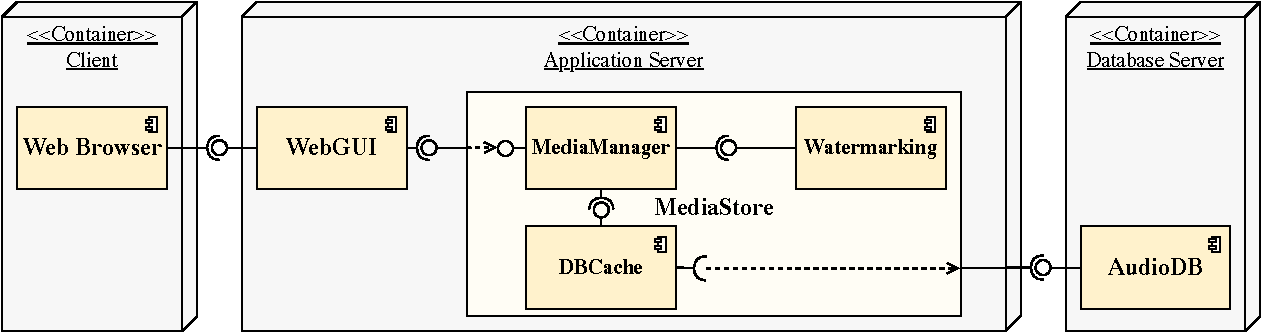
\includegraphics[width=0.99\linewidth]{figures/mediastore.pdf}
    \caption[Example Instance for the Modeling Assignment]{Component-based architecture of a media store, which the assignment's metamodel should be able to represent. Loosely based on the work of \citet{becker2008a}.}
    \label{fig:mediastore}
\end{figure} 

\textbf{Ethical Considerations:}
During this experiment, ethical considerations were given due attention. Participants voluntarily partook and were fully informed about the experiment's scope and purpose. They explicitly agreed to use and publish their artifacts for research purposes, ensuring confidentiality by anonymizing them.% Transparency and respect for participants were principles upheld during the study.

\subsection{Observed Results}
%\todo{(LOW) Examples aus Vortrag zu Figures machen.}


%\citet{Babur2019}:
%\begin{description}[style=unboxed,leftmargin=5pt]
%    \item[Type-A] Exact duplicates except for layout, formatting, internal ids, and cosmetic name changes (lower-/uppercase)
%    \item[Type-B] Duplicates with smaller syntactic/semantic changes to names, types, attributes, and minor additions/removals.
%    \item[Type-C] Duplicate larger changes/additions/removals of elements, names, types, and attributes.
%    \item[Type-D] Semantically duplicates with different structures and content.
%\end{description}

%\citet{Faidhi1987,Karnalim2016}:
%\begin{description}[style=unboxed,leftmargin=5pt]
%    \item[Level 0:] Verbatim copy.
%    \item[Level 1:] Changes in comments and indentation.
%    \item[Level 2:] Changes in names.
%    \item[Level 2.5:] Changes to packages and package namespaces (introduced by \cite{Karnalim2016}).
%    \item[Level 3:] Changes in declarations (e.g., adding extra constants, changing the positions of declared variables, shuffling the methods, etc.).
%    \item[Level 4:] Changes in pro wordgram modules (e.g., encapsulating statements in methods, using either parameters or global variables, inserting dummy methods).
%    \item[Level 5:] Changes in program statements (e.g., using FOR instead of WHILE, etc.).
%    \item[Level 6:] Changes in the decision logic (e.g., changes in expressions, loops to recursion, rearranging loosely coupled statements).
%\end{description}

\begin{table*}[t]
	\centering
    \small
	\begin{tabular}{l p{215pt} r r r} % nach letztem c @{\hskip 2em}
		\toprule
		Techniques         & Description                                                                       & \footnotesize\#Occ. & \footnotesize\#Part. & \footnotesize Type\\
		\midrule
		Cosmetic Renaming  & Changing capitalization of names, introducing or resolving typographical errors.                 & 1    & 1    & A                     \\
		Minor Renaming     & Introducing or resolving abbreviations, adding and removing suffixes or prefixes. & 85   & 9    & B                     \\
		Major Renaming     & Changing names to synonyms, translations, or entirely different names.            & 141  & 7    & C                     \\
		\midrule
		Reorder Features  & Re-ordering attributes and references of a classifier.                            & 10   & 1    & B                     \\
		Reorder Package   & Re-ordering the model elements contained within a single package.                       & 57   & 4    & B                     \\
		Reorder Classifiers & Moving classifiers from one package to another (re-ordering across the model).  & 1    & 1    & C                     \\
		\midrule
		Introduce Package  & Create a package and add existing elements from other packages or other packages. & 20   & 3    & C                     \\
		Dissolve Package   & Deleting a package and moving its contained elements to other packages.           & 8    & 4    & C                     \\
		\midrule
		Delete Feature     & Delete an existing attribute, relation, or operation of a classifier.             & 26   & 7    & B                     \\
		Delete Classifier  & Delete an existing classifier from the model.                                     & 11   & 6    & C                     \\
		Delete Package     & Delete an existing package from the model (can be part of dissolving a package).  & 5    & 4    & B                     \\
		\midrule
        Insert Feature     & Insert a new attribute, relation, or operation into a classifier.                 & 6    & 4    & B                     \\
		Insert Classifier  & Insert a new classifier into the model.                                           & 10   & 3    & C                     \\
		Insert Package     & Inserting a new package into the model (may be combined with moving elements).    & 5    & 4    & B                     \\
		\midrule
        Change Property    & Changing an element's property, e.g., \textit{abstract} for classifiers, \textit{ordered} or the cardinality for references. & 31    & 3    & B                     \\
		\midrule
		Remove Inheritance & Remove inheritance relation between the two classifiers.                          & 4    & 1    & C                     \\
        Add Inheritance    & Add inheritance relation between the two classifiers.                             & 7    & 2    & C                     \\
		Change Inheritance & Changing the inheritance hierarchy structurally without changing it semantically. & 9    & 2    & D                     \\
		\bottomrule
	\end{tabular}
    \caption[Obfuscation Techniques by Novice Modelers]{Overview of the obfuscation techniques employed by the participants, classified according to \citet{Babur2019}. We include how often each technique occurred across all participants (denoted as \textit{\#Occ}) and how many participants employed it (denoted as \textit{\#Part}).}
	\label{tab:student-obfuscation}
%\todo{Do we want the midrules? And if yes how to we want to separate? e.g. for property?}
\end{table*}



\noindent
%
In this section, we present our findings~\cite{Saglam2023_supp}, analyze the participants' obfuscation techniques, examine human plagiarism detection effectiveness, and evaluate an automated tool's detection performance.

\paragraph{Obfuscation Techniques}
To analyze the obfuscation techniques employed by the students, we first used \textit{EMF Compare} to identify potential differences between the plagiarized models and their originals. Unsurprisingly, in some cases, EMF Compare did not accurately produce the correct differences~\cite{Wittler2023}, highlighting the limitation of relying solely on model differencing for plagiarism detection.
In the second step, we thus manually inspected the models, carefully examining them for potential obfuscation. To ensure the validity of our observations, we cross-referenced our findings with the textual descriptions provided by the students.
 %
In our experiment, the participants engaged in a range of individual alterations to obfuscate the plagiarism, with the number of alterations varying between 10 and 91. Thereby, we count semantic alterations, e.g., moving an element as a single one. The mean number of alterations is 43.7, while the median is 31.5. These results imply an average of approximately one alteration for every two model elements in the source model.

We classify the participant's techniques according to the modeling clone types from \citet{Babur2019}, based on the \ac{UML} clone types of \cite{Stoerrle2015}.
While designed for clones rather than plagiarism, this classification enables systematic categorization of plagiarism techniques.
\citet{Babur2019} describe \textbf{Type-A} clones as exact duplicates except for layout, formatting, internal IDs, and purely cosmetic name changes.
\textbf{Type-B} clones have minor syntactic and semantic changes to names, types, attributes, and minor additions or removals.
\textbf{Type-C} clones include more extensive alterations, additions, and removals of elements and their properties.
Finally, \textbf{Type-D} clones are semantically equivalent with different structures and content.

We provide an overview of the techniques, indicating the frequency of their application and the number of participants who utilized each technique.
%
As summarized in \autoref{tab:jplag-student-obf}, the participants employed various obfuscation methods during the experiment. The types of changes can be described as follows:
The most common method was renaming, accounting for about half of the total changes made by all participants. Notably, the participants tended to utilize sophisticated renaming strategies, resulting in the majority of these alterations being categorized as \textit{major renaming} and none as \textit{cosmetic renaming}. 
As an example of such major renaming, one participant renamed a classifier from \textit{"Component"} to \textit{"BuildingBlock"}.
%
Other properties, such as \textit{abstract} or \textit{ordered}, were also subject to changes, albeit less frequently than names.

Another common practice observed was the reordering of elements. However, most participants refrained from moving classifiers across packages. Instead, they focused on rearranging the contents of the packages themselves or altering the order of features within the classifiers. Some participants also introduced or dissolved packages, thus moving the contained packages or classifiers.
%
Contrary to our initial assumptions, the insertion and deletion of elements were far less common than expected. While in source code assignments, the insertion of lines is one of the most prevalent obfuscation techniques~\cite{Novak2019}, our findings did not reflect this for modeling assignments. Deleting elements, particularly features, was observed slightly more frequently than insertions.
%
Four participants also modified the inheritance relations between classifiers. Interestingly, two students went beyond simple alterations and completely replaced the inheritance hierarchy with a different one while ensuring that the underlying semantics remained intact. This is the only technique we classified as \textit{Type D} (semantically equivalent, structurally different).
%
In summary, \autoref{tab:jplag-student-obf} shows that students employ diverse obfuscation techniques with varying frequencies.

\paragraph{Human Detectability}
To evaluate if humans can detect the participants' plagiarism instances, we asked the course instructor to review eight metamodels regarding their originality and whether they would accept them as valid solutions.
Due to time constraints, we only used a subset of the metamodels.
To include weaker and stronger instances of plagiarism, we selected the plagiarism instances based on the number of alterations made by the plagiarizers.
The subset for the review consists of four original solutions. It also contains three plagiarism instances derived from one solution and one instance from another.

For the review, we used the \textit{Think Aloud} method, asking the instructor to verbalize what they were thinking and doing. 
The instructor reviewed the models one after another, arranging them side-by-side and first checking for their overall structure and partition into packages. Within packages, they checked the order of elements and the naming of the elements, focusing on the data types that had to be modeled as part of the assignment. They also inspected the \ac{OCL} constraints contained for the models that seemed similar.
%
Within 20 minutes, they were able to identify all plagiarism clusters correctly. One of the plagiarized metamodels would not have been accepted as a valid solution as it is a poor translation of the original, resulting in nonsensical names. 
%
While the instructor identified all plagiarism instances correctly in this experiment, they also stated that this was possible only due to the small sample size. For more metamodels, they would be unable to compare them all manually side-by-side but would employ a tool. 

\paragraph{Tool-based Detectability}

\begin{figure}
    \centering
    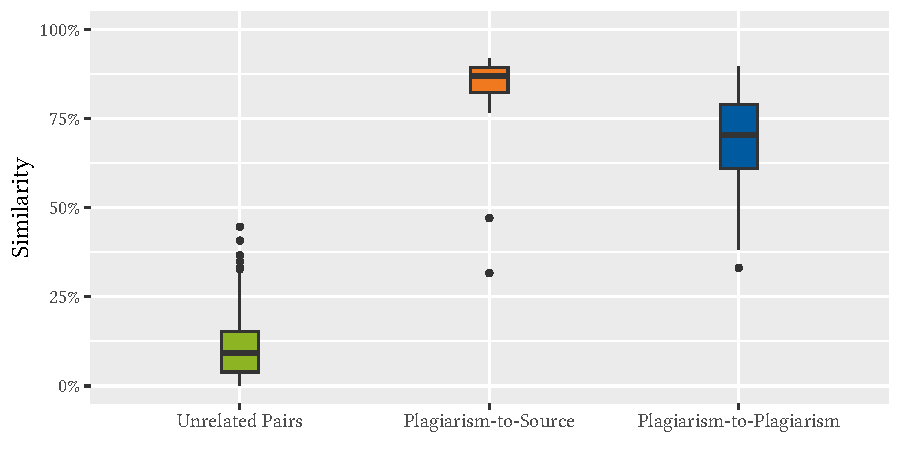
\includegraphics[width=\linewidth]{figures/mde/experiment_avg.similarity.pdf}
    \caption[Detecting Human Obfuscation]{Similarities computed by JPlag for unrelated pairs of original solutions, plagiarism instances with their sources, and plagiarism instances of the same source among each other.}
    \label{fig:jplag-student-obf}
\end{figure} 
    
\begin{table}[H]
		\centering
		\begin{tabular}{l cccccc}
			\toprule
			\textbf{Type}           & \textbf{Median} & \textbf{Mean} & \textbf{Minimum} & \textbf{Maximum} & \textbf{Q1} & \textbf{Q3} \\
			\midrule
			Unrelated\newline Pairs & 14.79        & 15.52         & 0.00         & 51.15        & 10.08       & 20.78       \\
			Plag.-to-Source         & 89.27        & 84.71         & 47.06        & 95.31        & 86.35       & 91.58       \\
			Plag.-to-Plag.          & 77.46        & 72.55         & 42.65        & 92.79        & 64.52       & 85.36       \\
			\bottomrule
		\end{tabular}
		\caption[Detecting Human Obfuscation]{Similarity metrics for the pair types in \autoref{fig:jplag-student-obf}, a higher difference to the unrelated pairs means better detection.}
		\label{tab:jplag-student-obf}
\end{table}

\noindent
To answer whether the plagiarized models can still be detected with a state-of-the-art tool, we employed the token-based plagiarism detector JPlag~\cite{prechelt2002, Saglam2022}.
To create a comprehensive labeled dataset, we combined the plagiarism instances from ten participants, along with their corresponding sources, and included unrelated solutions from previous years. This resulted in a dataset of 31 solutions, which we analyzed using JPlag.
%
JPlag computes similarities for each assignment pair, resulting in 465 pairs, which we depict in \autoref{fig:jplag-student-obf}.
Detecting the relationship between two instances of plagiarism from the same source is significantly more challenging than the relationship between a plagiarism instance and its source; as for the former case, the alterations made by both plagiarizers accumulate, leading to plagiarism up to twice as well obfuscated.
Thus, we separate them into distinct categories, illustrated in \autoref{fig:jplag-student-obf}.

The plagiarism-to-plagiarism pairs exhibit considerably lower similarities, with a median value of 77.5 percent, in contrast to the 89.3 percent for the plagiarism-to-source pairs. Furthermore, except for one outlier, all plagiarism-to-source pairs exhibit higher similarity values than all plagiarism-to-plagiarism pairs.
This outlier is the plagiarism instance by one participant, who achieves the reduced technique with two techniques. First, they were thorough, making 91 individual changes to the source model, corresponding to one change per model element. Second, they heavily relied on reordering model elements, a weakness of JPlag. Nonetheless, the similarity calculated by JPlag is high enough to detect this outlier.
%
Both groups, however, can be clearly distinguished from the pairs of unrelated models, which exhibit a significantly lower median similarity value of 14.8 percent.
In summary, our findings show that modeling plagiarism can be detected automatically.

%\noindent
%\textit{Lessons Learned:}
\subsection{Lessons Learned}
Our experiment revealed that despite the various types of changes, most students predominantly utilized renaming, deletion, and reordering as obfuscation techniques. This highlights the limitations of relying on names for plagiarism detection. In modeling, names hold significant importance compared to code, but they enable effortless obfuscation attacks for plagiarism. Similarly, unique identifiers cannot be solely relied on, as they can be manipulated, hindering the identification of plagiarized elements.
Detection tools should be designed to minimize the impact of easily manipulated characteristics of modeling artifacts.
%
Students rarely utilized type A changes, indicating their intention to refrain from employing overt modifications. They also utilized very few type D changes, which might be more common among experienced modelers.

We observed that the relation between two plagiarism instances of the same original is significantly more challenging to detect than the relations between the plagiarism instances to the original.
Although modeling plagiarism can still be detected by humans or via tools, it may become more challenging with increased time spent obfuscating or with more experienced students.
In our experiment, the instructor often relied on model elements overlooked during the participant's obfuscation attempts, such as \ac{OCL} constraints.
Furthermore, they also noted that manual comparison would be impractical for larger sample sizes, necessitating using a plagiarism detection tool.
The instructor also mentioned that, without a tool, they would not conduct plagiarism checks without an initial suspicion.
These findings emphasize the need for continuous improvement of tool-based detection methods.

%\textit{Limitations:}
\subsection{Threats to Validity}
We now discuss the threats to the validity of our experiment and the measures we took to address them, following standard guidelines in experimental research~\cite{Wohlin2012}.
%
\paragraph{Internal Validity}
Internal validity refers to whether there are influences that can unknowingly affect the analyzed variable concerning causality~\cite{Wohlin2012}.
%
Since this study was conducted in a simulated setting, the plagiarism behavior of the participants might not entirely reflect the complexity or effort of real-life instances. In a controlled environment, the level of effort students apply to conceal plagiarism may be lower than in actual academic settings, which could impact the frequency of the employed changes.
%
Nonetheless, we maintain that these conditions are adequate for observing \textit{how} students plagiarize.
%
\paragraph{External Validity}
External validity concerns the extent to which our findings can be generalized beyond the context of the experiment.
%
Furthermore, motivating students to participate in experiments presents a challenge. To address this, we kept the duration of the experiment relatively short. Nevertheless, the number of participants could be higher. Increasing the number of participants would improve generalizability across diverse educational settings.
%
The experiment used only a single modeling assignment, which may not capture the full range of potential plagiarism strategies. Incorporating assignments of varying complexity or different types, such as behavioral modeling languages (such as sequence diagrams), might reveal additional or unique plagiarism tactics.
%
Similarly, this experiment was limited to a single course conducted in one semester, constraining the variety of educational settings covered. Repeating the study across multiple courses or semesters could improve the generalizability of the results.
%
\paragraph{Construct Validity}
Construct validity refers to the degree to which we measure the theoretical construct we intend to measure.
%
Since the experiment involved only one type of assignment (an \ac{EMF} metamodeling assignment), construct validity may be limited. Including other assignment types, especially those beyond modeling, could help confirm whether the observed plagiarism techniques are specific to modeling or applicable to other domains. Nevertheless, \ac{EMF} widely used in modeling education and metamodeling assignments are typical~\cite{Ciccozzi2018}.
%
\paragraph{Reliability}
Reliability concerns the consistency and replicability of the results.
To ensure reliability, we have made all artifacts of the experiment available in a dedicated reproduction package~\cite{Saglam2023_supp}.
%
\paragraph{Conclusion}
Despite these limitations, the experiment provides valuable insights into techniques students use to plagiarize modeling assignments. These insights contribute to future research and inform the development of plagiarism detection mechanisms tailored to these unique challenges.

\section{Exploiting Generative AI for Modeling Plagiarism}\label{sec:ai-plagiarism}

In the previous section, we explored which techniques novice modelers employ to manually obfuscate artifacts of modeling assignments. We identified various techniques they employed to conceal their plagiarism and discussed the challenges this poses for detection. While these insights provide a valuable foundation on human obfuscation methods and highlight the complexity and creativity involved, it is crucial how such obfuscation techniques can be automated. The rapid advancement of generative artificial intelligence, particularly via \acp{LLM}, introduces a new dimension to this issue.

\acp{LLM}, such as \ac{GPT} and its successors, have demonstrated remarkable capabilities in generating and transforming text, including code and other structured data~\cite{Camara2023}. These models can potentially be exploited to cheat in modeling assignments~\cite{Biderman2022}. Given their ability to consider domain context and produce human-like modifications, the use of generative artificial intelligence might not be trivial to detect~\cite{Daun2023}.

Understanding how AI-based techniques can be leveraged to obfuscate modeling plagiarism will help us develop more robust detection mechanisms. In this section, we thus explore the potential use of AI for obfuscating modeling assignments.

\subsection{Feasibility and Techniques}
% INTRODUCTION
Although large language models have existed for some time, ChatGPT~\cite{ChatGPT} was the first to combine natural-language capacities with a simple user interface in the form of a chatbot.
This makes ChatGPT especially feasible for plagiarism, as other plagiarism generators~\cite{DevoreMcDonald2020} have been less approachable.
Thus, we investigate whether ChatGPT and other \ac{LLM}-based tools can be effectively exploited for plagiarism.
Unlike other plagiarism generators~\cite{DevoreMcDonald2020} and \acp{LLM} that have been less accessible, ChatGPT is widely available, easy to use, and popular among students \cite{ChatGPTGuide}. The techniques explored in this section, however, apply to other \acp{LLM} and tools based on generative AI, which allow for a natural language command as input, often referred to as prompt.
We show the feasibility of leveraging it for modeling plagiarism, requiring only a minimal understanding of modeling concepts.
%
% CHATGPT AND MODELING
Besides natural language capabilities, ChatGPT can describe, summarize, and generate programs and other technical artifacts, such as \ac{XMI}~\cite{Daun2023} code.
Thus, it can generate syntactically correct models for any language, often closely resembling a semantically correct solution created by humans." This can then be exploited for plagiarizing modeling assignments.
Based on our threat model (see \autoref{def:obfuscating-preexisting-solutions} and \autoref{def:assignment-driven-geenration}), there are generally two ways of using generative AI to cheat for modeling assignments:
\begin{enumerate}
    \item Assignment-Driven Generation: The plagiarizer uses the assignment's description to generate a complete solution using generative AI.
    \item Obfuscating Preexisting Solutions: The plagiarizer provides a preexisting solution and prompts generative AI to generate an obfuscated version.
\end{enumerate}
Whether the first technique constitutes plagiarism is still a subject of debate~\cite{Anders2023}, while the latter closely aligns with human plagiarism practices \cite{Novak2019}.
To determine how viable these approaches are, we explored both options\footnote{We used version 3.5 for the full generation, and version 3.0 and 3.5 for the obfuscation.} for a typical~\cite{Ciccozzi2018} metamodeling assignment~\cite{Saglam2022}.
It tasks students with creating an \ac{EMF} metamodel for designing component-based system architectures.

\subsection{Fully-Generating a Solution}

\label{subsec:chatgpt-full}
We tasked ChatGPT to generate a solution from scratch by providing the full assignment description (we converted the assignment PDF into plain text).
We used the metamodeling assignment regarding designing component-based system architectures, which we also used for our previously mentioned experiment (see \autoref{sec:human-plagiarism-task}).
For prompt engineering, we approached ChatGPT with the mind of a novice student modeler~\cite{Saglam2023}.
We systematically tested multiple prompts where the most expedient was directly asking for an \ac{EMF} metamodel that satisfies the description and is provided as syntactically correct XMI:
\begin{myquote}
    \textit{Please create an Ecore metamodel that meets the following description and provide its \ac{XMI} code with the correct syntax for opening the \ac{XMI} file via \ac{EMF} in Eclipse: [Assignment Text]}
\end{myquote}
Further inquiries, e.g., suggestions for improvement or correction, did not enhance the result quality\footnote{For details refer to \cite{Saglam2023} and \cite{Saglam2023_supp}.}.
Using this prompt, we conducted twenty sessions using two separate accounts. After each solution, we regenerated the next most likely response. We requested a single re-generation per session if it produced incoherent output, i.e., invalid \ac{XMI} code. 
In cases where ChatGPT stopped generating mid-model, we prompted it to continue.
%
Although we were able to generate 36 EMF-compatible solutions using ChatGPT, none fulfilled the assignment.
First, most of them contained a plethora of syntactical issues, including incorrect assignments of primitive types to attributes, improper assignment of reference types, duplicate names of structural features in types and super types, invalid lower bound cardinalities (e.g., a lower bound of -1), missing instance type names for enumerations, and packages lacking namespace \ac{URI} and prefix.
%
Second, all solutions were semantically insufficient, missing some essential elements. Incorrect modeling of relations between concepts and improper use of enumerations were common themes. Comparatively, the generated solutions contain about half as many classifiers and references as human solutions.

To evaluate the solutions regarding completeness and originality, we randomly selected a subset consisting of seven ChatGPT-generated and three human solutions and asked the course instructor to review them. The instructor was unaware that some of the metamodels were generated.
%
We asked the instructor to review the metamodels regarding their originality and whether they would accept the metamodels as valid solutions. We did not tell them that some of the metamodels were generated.
We employed the \textit{Think Aloud} method for the review, asking the instructor to verbalize their thoughts and actions.
%
This process is similar to the experiment setup described in~\cite{Saglam2023}, where we conducted a similar experiment on human plagiarism. We asked a course instructor to check metamodels regarding their originality and validity as a solution.
%
The instructor reviewed the solutions individually and arranged them side by side. They initially examined the overall structure and package partitioning. Within packages, they specifically checked for the presence of elements described in the task.
%
They accepted only the three human solutions, as the other solutions contained errors and missed crucial concepts of the assignment.
%
They noted that the generated solutions appeared similar, with small sizes and minimal structuring into packages.

The similarity can be attributed to the recurring patterns in correctly modeled concepts and the occurring syntactical and semantical issues.
ChatGPT exhibits some degree of determinism in its outputs, which is due to the inherent indeterminism in generative AI. While large language models are, by design, not entirely deterministic (their output variability is often controlled by parameters like \textit{temperature}, which influences the level of "creativity" in responses\footnote{Large language models achieve indeterminism through controlled randomness, mainly by using sampling methods over the most likely outputs and adjusting the temperature parameter. The temperature scales word probabilities by adjusting the probability distribution curve~\cite{Ouyang2023}.}); they exhibit a level of determinism that is strong enough that, given the same assignment, the outputs are similar enough for the context of plagiarism detection. Note that ChatGPT does not allow temperature control.
To further examine this, we used our approach to compare the similarity of generated and human solutions.
The results are shown in \autoref{tab:summary-fully}.
The values indicate that, despite their small size and issues, generated solutions are notably more similar than unrelated human solutions.
This shows that our approach can effectively detect many of these generated solutions.
In summary, fully generating solutions works for small assignments, but the results are inadequate and easily detectable.

\begin{table}
		\centering
		\begin{tabular}{lcccccc}
			\toprule
			{Type}             & {Median} & {Mean}  & {25\% Perc.} & {75\% Perc.} & {Maximum} \\
			\midrule
			Human   & 18.25        & 19.75          & 12.21       & 25.35   & 58.15    \\
			ChatGPT & 35.37        & 36.97          & 26.23       & 47.60    & 86.84  \\
			\bottomrule
		\end{tabular}
        \caption[Similarity of Human vs. AI-Generated Solutions]{Similarity in percent of unrelated human originals compared to the similarity of the solutions generated with ChatGPT.}
		\label{tab:summary-fully}
\end{table}


\subsection{Obfuscating a Preexisting Solution}

\label{subsec:chatgpt-obf}
To obfuscate a preexisting solution, we provide ChatGPT only with a solution in \ac{XMI} form and define a prompt with instructions to alter the structure of the solution to conceal the plagiarism while retaining semantics to fulfill the assignment.
We applied this approach to solutions from the modeling course: a monolithic one with all elements in a single file and a fragmented one with elements distributed across five files in various packages.
We generally observed a stronger obfuscation for the fragmented solution, which may relate to the semantic cohesion of the concepts modeled in the same package.
%
We applied twelve different prompts in independent sessions for each solution, thus generating twelve plagiarized metamodels.
The following is an example of such a prompt:
\begin{myquote}
%\small
\textit{Change the following \ac{EMF} metamodel in \ac{XMI} format to look like a different one that models the same concepts.
Show changed lines, including a description and the line number.}
\end{myquote}

% MODIFICATIONS ----------------------- 
%\noindent
ChatGPT employs various modifications to alter the solution, detailing what part of the \ac{XMI} code changed.
These modifications included inserting single classes, attributes, and references, deleting elements and their contained elements, re-ordering elements in containment references, and moving attributes or references to newly inserted superclasses. ChatGPT also moved classes and datatypes to different packages and renamed elements by abbreviating or removing abbreviations, using synonyms, or adding prefixes and suffixes based on the domain. Moreover, it changed the properties of existing elements, such as multiplicities, and added references to classes that referred to either existing or new classes. Vice versa, it added new classes containing multiple attributes and meaningful references to new and existing classes.
%
It often made complex changes by adding sizable structures that had semantic relevance to the solution's domain.
One example that arose multiple times included adding a new class named \texttt{Node} with a one-to-many relationship to the existing class \texttt{Links} and a many-to-one relationship to \texttt{Container}. Additionally, ChatGPT modified the \texttt{Links} class to depict a directed link between two nodes:
%
\begin{myquote}
     \textit{I added a new \texttt{EClass} called \texttt{Node} with a one-to-many relationship with \texttt{Links} and a many-to-one relationship with \texttt{Container}. The new class will represent the environment's nodes. Change the \texttt{Links} class to represent a directed link between two nodes. Add two references, \texttt{source} and \texttt{target}, to represent the endpoints.}
\end{myquote}

% EX 0
\noindent
In one example, ChatGPT inserted a new subclass \texttt{SystemComponent} of an existing class \texttt{Component} and added a reference \texttt{partOf} which referenced an existing class \texttt{System}.
% EX 1
In another one, a new abstract class called \texttt{NamedElement} with an attribute called \texttt{name} was inserted.
Then, it introduced this class as a supertype for several existing classes that removed their \texttt{name} attribute, effectively deduplicating the attributes.


Most of these changes are not immediately apparent, as they fit the assignment's domain.
Even if modeling issues occurred, they were insignificant enough to be considered plausible human mistakes.
Only in about one in ten cases were the changes immediately conspicuous, and for those instances, it was due to chosen element names lacking logical coherence (such as renaming from \texttt{Deployment} to \texttt{DeploymentNew}).
%
We found that ChatGPT generated minor syntactical issues (for example, type declaration that still references the original name of a renamed element) in some cases, but for the most part, it produced correct metamodels that were well-obfuscated according to our instructions.
In contrast to the technique of fully generating, ChatGPT seems to thrive on the given metamodel, thus avoiding most issues discussed in \autoref{subsec:chatgpt-full} by replicating what already exists.

%\todo{(LOW) Create figures for examples}

\subsection{Key Takeaways}

In summary, while we can fully generate solutions for modeling assignments with ChatGPT, they are inadequate, stand out to the human eye, and are likely to get flagged during tool-based inspection.
Recent studies reached the same conclusion \cite{Camara2023}.
However, given a preexisting solution, the usefulness of ChatGPT increases. It can convincingly summarize the modeled domain and its structure and concepts. Moreover, using ChatGPT allows us to perform complex changes, providing high flexibility in generating obfuscated models.
%
While fully generating solutions might become feasible in the future, cheating via plagiarism by obfuscation currently seems the most feasible strategy, as it requires little modeling knowledge and produces well-obfuscated plagiarism that is inconspicuous for humans.




\chapter[Modeling Plagiarism Detection]{Token-based Plagiarism Detection for Artifacts of Modeling Assignments}\label{sec:mde-approach}

\noindent
In this chapter, we address the problem of modeling plagiarism detection (\probref{2}) by introducing a novel approach to enable token-based plagiarism detection for modeling assignments (\contribution{2}). 
Where applicable, we reuse concepts of token-based approaches that are compatible with modeling artifacts, adapting only those components that are inherently incompatible with the unique characteristics of modeling languages.
With this, we provide resilience against obfuscation techniques and allow state-of-the-art token-based plagiarism detection systems to extend their scope beyond code-based approaches.
%
With this approach, we address the challenges discussed in \autoref{sec:mde-challenges}.

For our approach, modeling artifacts that are EMOF-conforming~\cite{MOF2016a} or that have an underlying tree-like structure are particularly suited, but our approach can be generalized beyond them. Supported modeling artifacts include (domain) models, metamodels, but also model transformations and model queries, as they can be represented as models themselves~\cite{Bezevin2005, Martinez2020},

The remainder of the chapter is structured as follows.
First, we discuss the difficulty of defining intrusiveness for modeling artifacts.
Second, we provide a minimal running example for the remainder of this chapter.
Next, we provide an overview of our approach. We explore the primary challenge of tokenizing modeling artifacts and examine the required normalization steps. We address the pairwise matching of subsequences, detail the similarity calculation, and the result visualization. Finally, we conclude with a discussion of the limitations.

\ownpublications{
    \fancycite{Saglam2024a},
    \fancycite{Saglam2023},
    \fancycite{Saglam2022}, and
    \fancycite{Kienzle2024}.
}

\section{Intrusiveness in Model Obfuscation}\label{sec:mde-intrusiveness}
As discussed in \autoref{sec:mde-challenges}, the differentiation between semantic-preserving, semantic-agnostic, and semantic-deviating obfuscation is blurred in the context of modeling plagiarism, as for metamodels dynamic semantics are often only informally specified~\cite{Brambilla2017}.
To address this issue, we thus distinguish two cases: 


If there is there are formally described dynamic semantics for a given metamodel, we can define the \textit{intrusiveness} (see \autoref{sec:intrusiveness}) analogous to \autoref{def:spoa}, \autoref{def:saoa} and \autoref{def:sdoa}, but instead of the functional equivalence as defined in \autoref{def:func-eq} we use the semantic equivalence of models:
\begin{theorem}[Semantical Equivalence of Models]\label{def:sem-eq}
Let \(M_1, M_2 \in \mathcal{M}\) be models of a metamodel \(\mathcal{M}\). 
We denote the semantic equivalence of two models \(M_1\) and \(M_2\) by the binary relation \(\equiv_{\mathcal{M}} \, \subseteq \mathcal{M} \times \mathcal{M}\).
% where \(M_1 \equiv_{\mathcal{M}} M_2\) iff \(M_1\) and \(M_2\) are semantically equivalent.
\end{theorem}

If there are no formally described dynamic semantics for a given metamodel, but we can define a transformation between the metamodel and a formalism with well-defined semantics, we can define derived semantic equivalence as follows.
\begin{theorem}[Derived Semantical Equivalence of Models]\label{def:sem-eq-derived}
Let \(M_1, M_2 \in \mathcal{M}\) be models of the metamodel \(\mathcal{M}\). Furthermore, let \(\mathcal{P}\) be a formalism with well-defined semantics and let \(P_1, P_2 \in \mathcal{P}\) be representations of \(\mathcal{P}\) for which semantical equivalence is denoted by the binary relation \(\equiv_\mathcal{P} \, \subseteq \mathcal{P} \times \mathcal{P}\).
Suppose there exists a transformation \(t: \mathcal{M} \rightarrow \mathcal{P}\) such that
\[
M_1 \xrightarrow{t} P_1 \quad \text{and} \quad M_2 \xrightarrow{t} P_2 \,.
\]
Then, we define the derived semantic equivalence on \(\mathcal{M}\) as follows:
\[
P_1 \equiv_{\mathcal{P}} P_2 \quad \implies \quad M_1 \equiv_{\mathcal{M}} M_2.
\]
\end{theorem}

As for program code, the distinction regarding intrusiveness in the context of models is useful, as it allows categorizing and reasoning about different types of obfuscation attacks. However, a difference between any two models, for example, derived via model differencing, that reflects a semantic-preserving change is not evidence for obfuscation. It is actually impossible to categorically decide which types of differences between the two models constitute obfuscation and are thus formal evidence for plagiarism, even under a clear definition of intrusiveness. Plagiarism detection must \textit{always} involve human inspection at the end, where this decision is made on a case-by-case basis (see \autoref{sec:foundations-pds}).

\section{Running Example}
\label{sec:mde-example}

\begin{figure}[b]
    \centering
    \begin{subfigure}{.96\textwidth}
        \centering\captionsetup{width=.95\linewidth}%
        \caption{First example metamodel.}
        \label{fig:sub1}
        %\includegraphics[width=.89\textwidth]{images/bookStore2.pdf}
        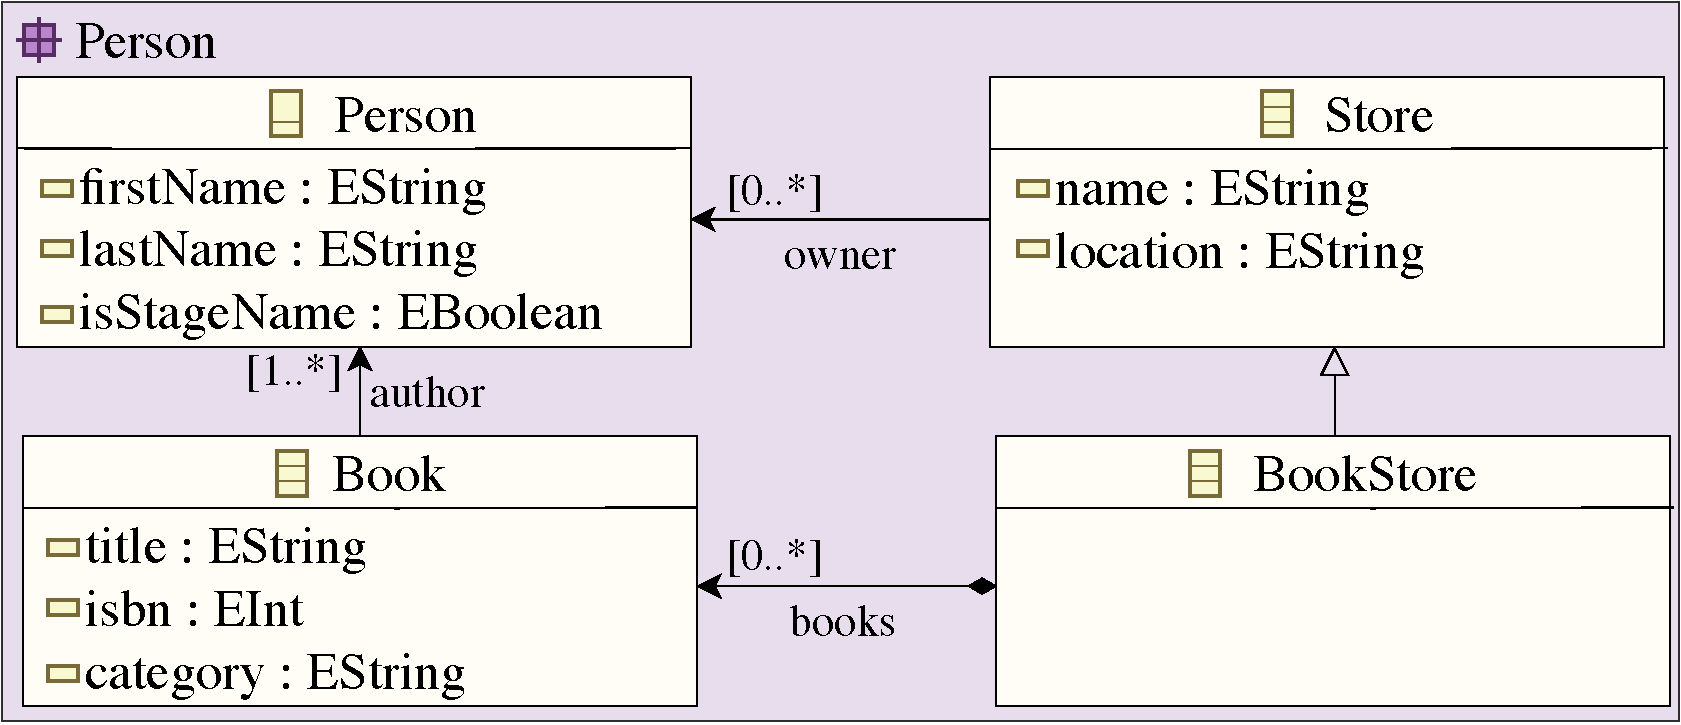
\includegraphics[width=.8\textwidth]{figures/mde/bookstore-1.drawio.pdf}
    \end{subfigure}  
    
    % This comment needs to stay, or the figures will not be side-by-side. Yes, this is not a joke. 
    \begin{subfigure}{.96\textwidth}
          \centering\captionsetup{width=.95\linewidth}%
        \caption{Second example metamodel.}
          \label{fig:sub2}
          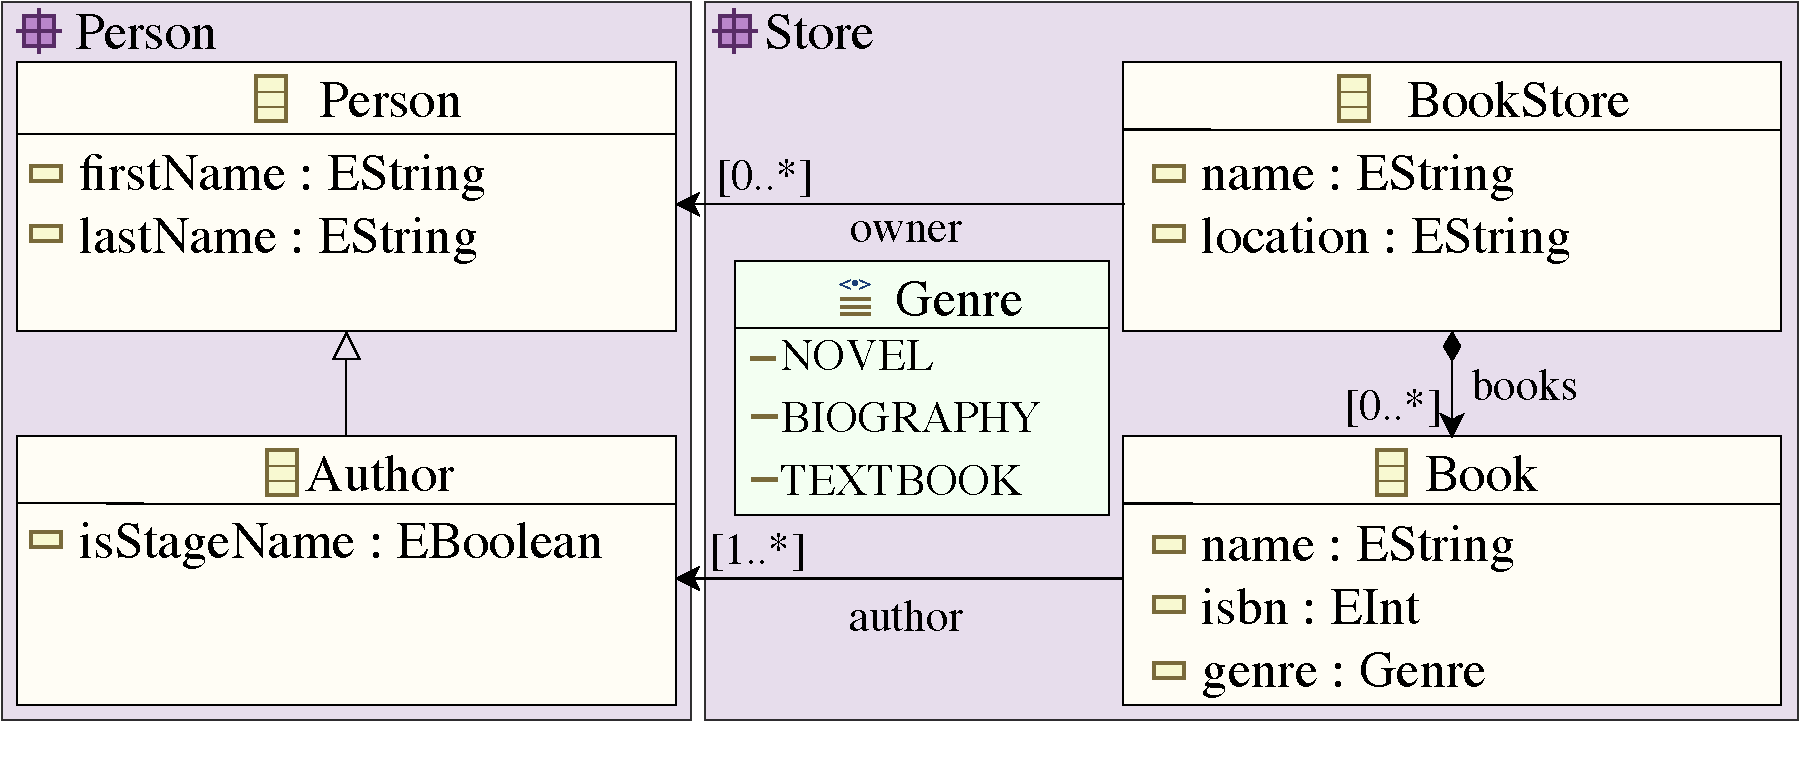
\includegraphics[width=.8\textwidth]{figures/mde/bookstore-2.drawio.pdf}
    \end{subfigure}
    \caption[Running Example: Bookstore Models]{Two similar but not identical example models representing a bookstore management system that allows managing multiple stores and their inventory.}
    \label{fig:running-example}
%\end{figure*}
\end{figure}
%
% SETUP
\noindent
As a minimal running example, we consider an undergraduate course where students are instructed in the elementary principles of modeling. Such a course is typical according to the survey of \citet{Ciccozzi2018}.
In order to satisfy the course requirements, they need to complete an assignment that entails modeling a management system for bookstores, requiring the creation of an appropriate metamodel.
% DOMAIN
The domain is described as follows:
\begin{myquote}
\small
\textit{Bookstore can have multiple locations that sell different books.
Books are classified into different genres and have a unique identifier called an ISBN.
Books have an author who may use a stage name. Stores have one owner.  }
\end{myquote}
This example is intentionally small to illustrate our approach and provide clarity for the reader; most modeling assignments are usually more comprehensive.
Two potential solutions for this assignment are depicted in \autoref{fig:running-example}.
% PROBLEM
Although they exhibit some similarities, several features are modeled differently.
While this is a small task, it is hard for a human to determine how similar these models are even for these two solutions.
However, in a course, there may be 30 to 300 students~\cite{Ciccozzi2018}. Thus, manual checking for plagiarism becomes impractical.
%\todo{expand? What is different? What are the similarities? Obviously, as a running example, it is too small to label something plagiarism, but it is still very complex to assess similarity.}

\section{Overview}\label{sec:mde-approach-overview}
The similarity between models and code can be leveraged for token-based approaches for modeling artifacts \cite{Saglam2022}.
These approaches typically extract tokens from parse tree nodes, primarily focusing on the code's structure.
In contrast, for modeling plagiarism, the focus must be on modeling patterns, structure, and relationships.
A key challenge is the higher abstraction than code, where the lack of details impedes plagiarism detection.
Furthermore, resilience against re-ordering-based obfuscation attacks is challenging.
Re-ordering-based attacks are more common \cite{Saglam2023} as they are considerably more accessible for most models than for code, where the sequence of statements determines the code's behavior.
% MODEL vs. CODE END
In our approach, modeling assignment solutions undergo a comprehensive pairwise comparison process.
To facilitate this comparison, an abstraction layer is extracted from each solution, on which the structures of these artifacts are compared.
Ultimately, our approach produces a list of suspicious solutions, which are the subject of the instructor's final evaluation.
% HUMAN FACTOR
As with all plagiarism detection systems, the human component of the process is critical for ethical reasons, as it can ultimately only be up to the instructor to decide whether a submission constitutes plagiarism~\cite{Culwin2001, Weber2019}.
Our approach combines the strengths of automated analysis with human judgment, offering an ethical approach to detecting plagiarism in modeling assignments.
%
% APPROACH OVERVIEW
As other token-based approaches~\cite{prechelt2002, Maertens2022}, our approach consists of five steps.
\begin{enumerate}%[leftmargin=*]
    \item \textbf{Tokenization}: We generate the token sequence by linearizing the model, extracting tokens for particular model elements, and abstracting from superfluous detail.
    \item \textbf{Normalization}: We achieve resilience against element reordering by normalizing the token sequence. This can be combined with other normalization techniques.
    \item \textbf{Pairwise Matching}: We efficiently compare pairs of token sequences to find the longest matching subsequences greedily, thus matching fragments of modeling artifacts.
    \item \textbf{Similarity Calculation}: We rank the pairs by leveraging different similarity metrics for the matches of a pair. Post-processing steps, such as clustering analysis, can be applied.
    \item \textbf{Visualization}: We visualize matching fragments between modeling artifacts via textual syntaxes to help educators assess the results and decide what constitutes plagiarism effectively.
\end{enumerate}
The novelty of our approach lies in steps 1, 2, and 5, while steps 3 and 4 are established techniques from token-based plagiarism detection.

% ------------------------------------------------------------------
% 1. TOKENIZATION
% ------------------------------------------------------------------

\section{Tokenization}\label{subsec:tokenization}


\noindent
Modeling assignments include diverse artifacts like metamodels, models, and other artifacts~\cite{Ciccozzi2018}, all vital in the modeling process.
Most of these artifacts are typically systematized in a tree-like structure. Throughout this section, we will mainly refer to models and their elements. However, our approach applies to other tree-based modeling artifacts, such as metamodels, et cetera.
%
Our approach transforms the modeling artifacts into an abstraction layer on which pairwise comparison can be performed. By omitting \textit{some} details while including others, mainly structural information, this abstraction layer is resilient against certain obfuscation attacks such as renaming and re-typing.
For example, we omit the names of elements and the exact types of attributes, as they are usually the first to be changed for obfuscation purposes~\cite{Saglam2022, Saglam2023}.
%
To tokenize models of a given modeling language, one first has to identify the primary \textit{tokenization references} in the modeling language.
%
\begin{concept}[Tokenization References]\label{def:semantic-ref}
    In the context of modeling plagiarism detection, the explicit references or connections within a model define its semantic aspects, dictating the meaning and behavior of the model elements. They are domain-specific relationships between elements within a model that influence the interpretation or execution behavior of the model. They are crucial for tokenization and thus have to be identified for each modeling language or domain. We call them tokenization references.
\end{concept}
%
These references are crucial in both structural and behavioral models. In structural models, tokenization references typically take the form of containment relationships, defining the hierarchical organization of elements. 
Tokenization references can take various forms in behavioral models, including dynamic references such as state transition references in state charts. Tokenization references are used to determine the order in which to tokenize the model elements.

\begin{theorem}[Tokenization]\label{def:tokenization}
Let \(M \in \mathcal{M}\) be a model which is an instance of Metamodel \(\mathcal{M}\) with elements \(\mathcal{E}_M\), and let \(\mathcal{C}_\mathcal{M}\) denote the set of metaclasses in the metamodel.
We define a left total relation, where \( \mathcal{T}_\mathcal{M} \in \mathbb{N} \cup \{\bot\} \) is the set of possible tokens for \(\mathcal{M}\),
\begin{align*}
    \operatorname{tokenize}_\mathcal{M}: \mathcal{E}_M \rightarrow \mathcal{T}_\mathcal{M}
\end{align*}
that assigns either a token \( t \in \mathcal{T}_\mathcal{M} \) or no token \( \bot \) to each element \( e \in \mathcal{E}_M \).
\end{theorem}

In our approach, we tokenize as follows:
\begin{enumerate}
    \item We iterate in a depth-first order over the tree structure of the model's tokenization references, starting from its root element.
    \item For each element, we decide what tokens may be extracted. The extraction strategy can either be generic or domain-specific.
    \item Token sequences from multiple files or artifacts are concatenated into one token sequence but separated via a pivot token.
\end{enumerate}

\autoref{alg:model-tokenization} shows such an algorithm for tokenizing models, which incorporates the three aforementioned steps.
Here, the function \textsc{Tokenize} is a mapping that provides a token for any given model element or no token (\(\bot\)) if none shall be extracted for a given element (see \autoref{def:tokenization}).
In the case of multiple root elements, the token sequence of the corresponding root elements can be concatenated.

\begin{algorithm}[H]
\caption{Recursive Tokenization of a Model}
\label{alg:model-tokenization}
\begin{algorithmic}[1]
\Require Model $M$ with root element $r$
\Ensure Token sequence \((t_i)_{i=1}^{l}\) representing the model $M$
\State Initialize empty token sequence: $(t_i) \gets (\,)$
\Function{TokenizeModel}{$r, (t_i)$}
    \State $(t_i) \gets (t_i) \, \cdot$ \textsc{Tokenize}$(r)$

    \For{each Element $e$ reference via tokenization references of $r$}
        \State $(t_i) \gets (t_i) \, \cdot$ \textsc{TokenizeModel}$(e, (t_i))$
    \EndFor
    \State \Return $(t_i)$
\EndFunction
\end{algorithmic}
\end{algorithm}

\noindent
As an example, \autoref{fig:tokenization} illustrates the tokenization for the domain of \ac{EMF} metamodels using our running example. In the case of \ac{EMF} metamodels, the tokenization references are the \textit{containment references}. The metamodel is depicted in a typical tree view, where the indentation signifies the containment relations.
The token tree (\autoref{fig:tokenization:sub1}) is linearized into a token sequence according to \autoref{alg:model-tokenization} (\autoref{fig:tokenization:sub2}). Each token represents information from the structure of the metamodel and is thus an abstract representation of the metamodel.

%We discuss two kinds of strategies for selecting tokens: 
There are generally two possible types of strategies for mapping modeling elements to tokens (which is the role \textsc{Tokenize} fulfills in \autoref{alg:model-tokenization}): \textit{generic strategies} and \textit{domain-specific strategies}.
%
The first kind is \textit{generic strategies}, where a token is extracted for each model element, and the identity of the token is the type of the element, the metaclass, respectively.

\begin{theorem}[Metaclass Instantiation]
Let \(M \in \mathcal{M}\) be a model which is an instance of Metamodel \(\mathcal{M}\) with elements \(\mathcal{E}_M\), and let \(\mathcal{C}_\mathcal{M}\) denote the set of metaclasses in the metamodel. For each element \( e \in \mathcal{E}_M \), there exists a unique metaclass \( C \in \mathcal{C}_\mathcal{M} \) such that \(e\) is an instance of \( C \). We denote this right-unique relationship with the operator
\begin{align*}
:: \, \subseteq \mathcal{E}_M \times \mathcal{C}_\mathcal{M} \,.
\end{align*}
\end{theorem}

\begin{theorem}[Generic Tokenization Strategy]\label{def:generic-strat}
Let \(M \in \mathcal{M}\) be a model which is an instance of Metamodel \(\mathcal{M}\) with elements \(\mathcal{E}_M\), and let \(\mathcal{C}_\mathcal{M}\) denote the set of metaclasses in the metamodel.

We define a surjection \( \operatorname{tokenize}_{generic}: \mathcal{E}_M \rightarrow \mathcal{T}_\mathcal{M} \), where \( \mathcal{T}_\mathcal{M} \) is the set of possible tokens for \(\mathcal{M}\), that assigns a token \(t_C \in \mathcal{T}_\mathcal{M}\) based on metaclass \( C \in \mathcal{C}_\mathcal{M} \) to each element \( e \in \mathcal{E}_M\) such that
\begin{align*}
    \forall e \in \mathcal{E}_M, \; \exists_1 t_C \in \mathcal{T}_\mathcal{M} \quad : \quad 
    \operatorname{tokenize}_{\text{generic}}(e) = t_C \iff e :: C \,.
\end{align*}
\end{theorem}
However, the generic strategy as defined in \autoref{def:generic-strat} has certain limitations. Some model elements are irrelevant and should not be extracted as tokens, as they increase the noise in the token sequence and can be used to obfuscate plagiarism. Additionally, the properties of elements are not represented in the token sequence at all. If these properties are semantically relevant, this leads to a lack of representation in the token sequence. When considering \ac{EMF} metamodels as an example, classes and interfaces are differentiated by a property.
While this generic strategy can be applied to any modeling language and thus to any modeling assignment artifacts, it may perform worse for a distinct domain than a strategy specifically tailored to one domain. However, a generic strategy may perform well enough for some modeling languages (mostly those where the essential information is provided by the model elements instead of their properties and relations). 

The second kind type of strategy is \textit{domain-specific strategies}, where the selection of tokens is designed for a single domain or modeling language.
This allows more fine-grained rules for mapping model elements to tokens. Thus, \autoref{def:generic-strat} no longer applies, as there is not necessarily a bijective mapping between metaclasses and token types. In the following, we discuss several possible rules that allow deviating from a generic tokenization strategy.

\begin{theorem}[Token Omission]\label{def:token-omission}
Let \( \operatorname{tokenize}_\mathcal{M}: \mathcal{E}_M \rightarrow \mathcal{T}_\mathcal{M} \) be a tokenization function according to \autoref{def:tokenization}. 
We refer to \( \operatorname{tokenize}_\mathcal{M}\) as a tokenization function with token omission if there is a model element\( e \in \mathcal{E}_M \) which does not map to any token, and thus the following applies:
\begin{align*}
       \operatorname{tokenize}_\mathcal{M}(e) = \bot \,.
\end{align*}
\end{theorem}

Model elements that can be omitted without changing the semantics of a model should not tokenized, as these elements can be exploited to affect the token sequence via an obfuscation attack. To that end, a token omission rule can be employed. This can be useful, for example, for typed elements, where the type should not be extracted as a token.
\autoref{fig:tokenization} illustrates an exemplary domain-specific tokenization for \ac{EMF} metamodels. As seen in \autoref{fig:tokenization:sub2}, we extract tokens for attributes, but no tokens are extracted for the values of these attributes.

\begin{theorem}[Token Collision]\label{def:token-collision}
Let \( \operatorname{tokenize}_\mathcal{M}: \mathcal{E}_M \rightarrow \mathcal{T}_\mathcal{M} \) be a tokenization function according to \autoref{def:tokenization}. 
We refer to \( \operatorname{tokenize}_\mathcal{M}\) as a tokenization function with token collision if there is a pair of distinct elements \( e_1, e_2 \in \mathcal{E}_M \), where \( e_1 \) and \( e_2 \) belong to different metaclasses \(C_1, C_2 \in \mathcal{C}_\mathcal{M}\) with \( e_1 :: C_1, \, e_2 :: C_2, \, C_1 \neq C_2 \) but produce the same token \(t \in \mathcal{T}_\mathcal{M}\) and thus the following applies:
\begin{align*}
       \operatorname{tokenize}_\mathcal{M}(e_1) = \operatorname{tokenize}_\mathcal{M}(e_2) \, .
\end{align*}
\end{theorem}

Two elements of a different type that can be used interchangeably without changing the semantics of the modeling artifact should map to a token with the same identity. To that end, a token collision rule can be employed.
Consider a metamodel for component-based software modeling as an example. If there are different ways of modeling a component, for example, via classes or via packages, but for the sake of the modeled architecture, they can be used interchangeably, then they should map to the same token representing components.

\begin{theorem}[Token Distinction]\label{def:token-distinction}
Let \( \operatorname{tokenize}_\mathcal{M}: \mathcal{E}_M \rightarrow \mathcal{T}_\mathcal{M} \) be a tokenization function according to \autoref{def:tokenization}. We refer to \( \operatorname{tokenize}_\mathcal{M}\) as a tokenization function with token distinction if there is a pair of distinct elements \( e_1, e_2 \in \mathcal{E}_M \), where \( e_1 \) and \( e_2 \) belong to the same metaclasses \(C \in \mathcal{C}_\mathcal{M}\) with \( e_1 :: C, \, e_2 :: C\) but produce different tokens \(t_1, t_2 \in \mathcal{T}_\mathcal{M}\) based on, for example, their values for a property of \(C\). Thus, the following applies:
\begin{align*}
       \operatorname{tokenize}_\mathcal{M}(e_1) \neq \operatorname{tokenize}_\mathcal{M}(e_2) \, .
\end{align*}
\end{theorem}

In contrast, elements of the same type that, through their properties, have different semantics should be mapped to different tokens.
To that end, a token distinction rule can be employed.
Note that a tokenization function can have token distinction, token collision, and token omission, as it consists of a set of mapping rules from model elements to tokens.
As seen in \autoref{fig:tokenization:sub2}, attributes and identifier attributes are extracted as different tokens, even though both are instances of the same metaclass. Here, the property of the attribute defines whether it is an identifier or not.
Similarly, this is done for references and containment references.
Finally, properties themselves may lead to the extraction of tokens, for example, for supertype references or similar (see \autoref{fig:tokenization:sub2}).

In summary, tokenization requires finding a suitable mapping between the set of model elements of a modeling language and a set of tokens, as defined by \autoref{def:tokenization}, to maximize the detection quality and obfuscation resilience. This has to be done for each modeling language or domain, as there is no universal mapping for all languages that fulfill this task. Ideally, finding such a mapping involves a domain expert in order to consider the particularities and ambiguities of that domain.
%
Selecting how model elements map to tokens for tokenization in token-based plagiarism detection requires careful consideration of the relevant elements and properties of the domain. A domain-specific strategy allows for a more fine-grained tokenization and is thus generally preferred. A generic strategy, however, remains a baseline for domains without a domain-specific strategy.

\begin{figure}
    \centering
    \begin{subfigure}{.45\linewidth}
        \centering\captionsetup{width=.99\linewidth}%
        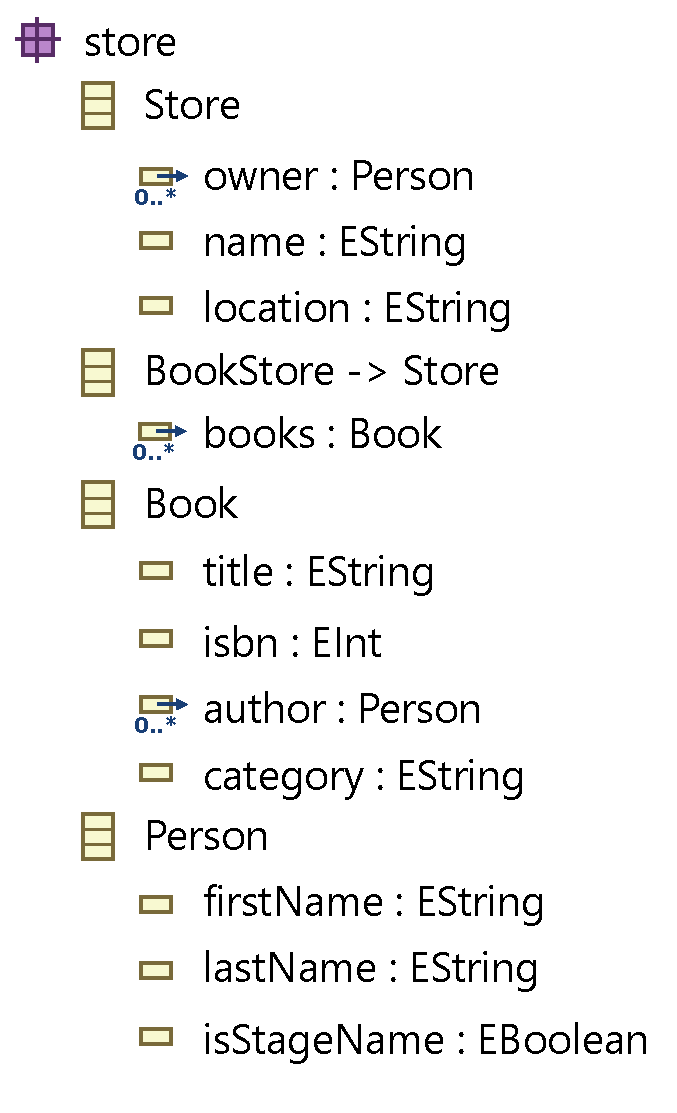
\includegraphics[width=.90\textwidth]{figures/mde/emfTreeView.pdf}
        \caption{first example metamodel}
        \label{fig:tokenization:sub1}
    \end{subfigure}% This comment needs to stay, or else the figures will not be side-by-side. Yes, this is not a joke.
    \begin{subfigure}{.45\linewidth}
          \centering\captionsetup{width=.99\linewidth}%
          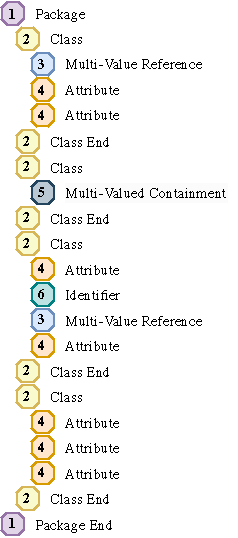
\includegraphics[width=.65\textwidth]{figures/mde/tokenSequence.pdf}
          \caption{extracted token sequence}
          \label{fig:tokenization:sub2}
    \end{subfigure}
    \caption[Tokenization of Modeling Artifacts]{Tokenization of one of the example models in \autoref{fig:running-example} to extract a linear token sequence as an abstraction layer for the comparison.}
    \label{fig:tokenization}
\end{figure}

\subsection{Tokenizing EMF Metamodels}
To continue our running example, we now discuss how to tokenize \ac{EMF} metamodels. This enables, for example, plagiarism detection for modeling assignments such as the one described in \autoref{sec:human-plagiarism-task}. However, these tokenization rules can be adapted for similar structural models with little effort. For example, the rules can be directly transferred to \ac{UML} class models, as \ac{EMF} is EMOF-compliant. As previously mentioned, in the case of \ac{EMF} metamodels, the tokenization references are the containment references. We discuss both a generic and a domain-specific strategy.

\subsubsection{Generic Strategy}
For the generic Strategy, we define the set of possible tokens based on the concrete metaclasses of the meta-metamodel as described in \autoref{def:generic-strat}.
To extract the tokens, we traverse the metamodel and extract tokens containing only the metaclass of the element as information. Properties like the element name are not transferred. This approach thus extracts tokens for packages, classifiers, attributes, references, etcetera.
\autoref{fig:ecore-tokenization} visualizes the inheritance tree of the Ecore meta-metamodel. The information extracted by the generic token selection is shown in blue and green. As the Ecore meta-metamodel is self-describing and self-instantiating, the generic token selection can be applied to their instances in addition to metamodels.
%
However, the generic token selection comes with two downsides.
As a first problem, it also extracts tokens with very little meaning. We observed \texttt{EGenericType} to be especially problematic, as \ac{EMF} automatically creates an \texttt{EGenericType} for every \texttt{ETypedElement} in a metamodel.
As a second problem, some vital information is not transferred into tokens. \ac{EMF} distinguishes concrete classes, abstract classes, and interfaces via two flags stored as attributes in the metaclass \texttt{EClass}.
Thus, the generic token selection only extracts class tokens and cannot make a more precise distinction. Analogously, containment references are not distinguished from regular references, and identifier attributes are not distinguished from regular attributes.

\subsubsection{Domain-Specific Strategy}
The domain-specific token strategy builds upon the previous strategy. It also uses metaclasses to extract tokens. However, it employs several tokenization rules for several types of model elements.
Compared to the generic strategy, there are three key differences in the token set:
\begin{enumerate}
    \item \textit{Stricter Token Selection}. The concrete metaclasses \texttt{EFactory}, \texttt{EGenericType}, and \texttt{EObject} are not extracted as tokens. They provide superfluous information as they are rarely explicitly modeled by a student. Thus, they needlessly increase the attack surface by allowing changes to the token sequence that do not alter the semantics of the metamodel (these are token omission rules as defined in \autoref{def:token-omission}).
    \item \textit{Token Distinction via Attributes}. Some concrete metaclasses are further distinguished to extract more fine-grained information. An \texttt{EClass} can be a class, abstract class, or interface. Containment references have a different token type compared to non-containment ones. Analogously, identifier attributes differ from normal attributes. This distinction broadens the token set and thus reduces false positives, as the discerned model elements semantically serve very different purposes (these are token distinction rules as defined in \autoref{def:token-distinction}).
    \item \textit{Extraction from Meta-References}. Some tokens are extracted for important meta-references in the Ecore meta-metamodel. Each superclass reference of an \texttt{EClass} is extracted as \textit{super type} token, and a return type reference of each non-void \texttt{EOperation} is extracted as \textit{return type} token (this is not possible via a generic strategy, as these references are not classes).
Again, these additional tokens reduce false positives. Moreover, they allow the detection of additional similarities, like the number of declared supertypes.
\end{enumerate}
%
As depicted in \autoref{fig:ecore-tokenization}, fewer concrete metaclasses are used for tokens. However, additional information is used to distinguish more token types.
In contrast to the generic token selection, this domain-specific strategy is tailored explicitly towards metamodels and thus not applicable to their instances. However, while it tends to extract fewer tokens than the generic strategy for the same input, it can differentiate between more token types through its refined and extended token set.


\begin{figure}
    \centering
    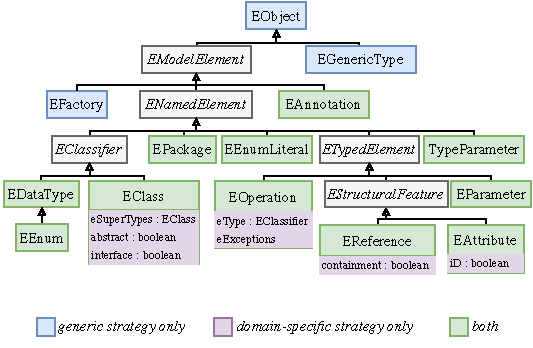
\includegraphics[width=0.85\linewidth]{figures/mde/Ecore-Both.pdf}
    \caption[EMF Metamodel Tokenization Strategies]{Tokenization rules for \ac{EMF} metamodel elements via the generic and domain-specific tokenization strategies illustrated for the Ecore metaclass hierarchy.}
    \label{fig:ecore-tokenization}
\end{figure}


\subsection{Tokenizing Behavioral Models}
Tokenization is more challenging for some modeling languages due to their complexity and the gap between their syntax and semantics. Many languages, especially those with less pronounced hierarchy but highly interconnected elements, are challenging to tokenize (see \autoref{sec:mde-challenges}). This difficulty is more pronounced for behavioral models.

The primary difficulty for behavioral models is identifying suitable tokenization references (see \autoref{def:semantic-ref}).
State transitions can be used for state charts, control flow edges can be used for activity models, and messages are suitable tokenization references for sequence models. However, it is not trivial to identify suitable tokenization references for all modeling languages. Yet, this challenge is part of designing a suitable tokenization strategy for new modeling languages. Thus, a domain expert must find a domain-specific tokenization strategy for each modeling language.

While proposing different concrete tokenization strategies for behavioral models is out of the scope of this dissertation, we discuss an example for \ac{SCXML}. \ac{SCXML} is a standardized language created by the World Wide Web Consortium (W3C) for specifying state machines. These examples show how a possible strategy might differ from structural models but not prescribe universal rules for behavioral models.

According to the SCXML metamodel, all states are contained in a single container element. This results in a relatively flat model hierarchy, which is little relevant for plagiarism detection.
Thus, for SCXML state charts, the containment relations are not the tokenization references.
Instead, the primary tokenization references are state transitions. Thus, we linearize starting from the starting state denoted with the \textit{initial} attribute.

To tokenize SCXML state charts, we consider states, transitions, events, and actions, thus representing the key components that define the behavior and structure of the state chart.
States are identified by their distinct keywords, allowing us to differentiate between initial, atomic, and compound states.
Transitions between states are tokenized based on event triggers, guards, and actions associated with state changes. By considering transitions, we extract relevant information such as the triggering event, conditions (guards) that govern the execution of transitions, and actions to be performed upon transition completion.

These transition tokens encapsulate the dynamic aspects of the state chart, illustrating how states interact and evolve in response to external events.
We consider not only the elements of the state chart but also the attributes and properties associated with them. Attributes influencing the tokenization process include boolean flags, which indicate characteristics like whether a state is parallel or composite, and enumeration values that describe types of transitions or other specific states of elements within the state chart. These attributes are directly mapped to tokens during the token extraction process.
Additionally, we preserve hierarchical relationships between states, allowing us to represent the nested structure. This hierarchical representation is essential for understanding the containment and nesting of states within compound states.
Note that this is a high-level overview of the tokenization rules. For a more comprehensive explanation, please refer to the work of \citet{Strittmatter2023}.

% ------------------------------------------------------------------
% 2. NORMALIZATION
% ------------------------------------------------------------------

\section{Normalization}\label{subsec:normalization}

\noindent
While the token sequence is resilient against obfuscation attacks such as renaming or re-typing, it is prone to other obfuscation attacks~\cite{DevoreMcDonald2020}. For modeling artifacts, this especially involves obfuscation attacks based on moving and swapping elements~\cite{Saglam2022} because most models allow variations in the order of multi-valued tokenization references.
%
Therefore, it is crucial to employ a normalization step.
Here, we normalize the order of the token sequence via the tokenization references and, thus, order the model tree while extracting tokens to ensure that the same patterns are represented identically across different modeling artifacts.

Normalization of the token sequence is a nontrivial task, as the properties used for normalization must be carefully chosen to avoid introducing new attack vectors while minimizing changes to the token sequence to prevent false positives. For instance, relying on properties like names, identifiers, or aggregated attributes can make normalization susceptible to manipulation through renaming or insertion attacks, ultimately affecting the token sequence. For example, sorting elements lexically by their names may prevent reordering-based attacks but remain vulnerable to renaming, where minor name changes alter the element order. Similarly, relying on properties like identifiers, types, or values can also lead to vulnerabilities. 

Only \textit{robust} criteria can provide stability and invariance to obfuscation attacks.
Robust criteria must exhibit stability under obfuscation and rely on information already used by the plagiarism detector. This limits robust normalization to structural and semantic patterns within the token sequence.
Thus, robust normalization avoids relying on properties that can be easily manipulated and instead focuses on intrinsic relationships within the extracted token sequences. This ensures that the normalization process does not introduce new vulnerabilities and remains effective across various obfuscation attacks.

The normalization step may contain various normalization techniques and defense mechanisms. In an upcoming chapter, we will discuss our normalization against subtree reordering and other defense mechanisms (see \autoref{cha:defense}).

\section{Pairwise Matching}
\label{subsec:matching}

\noindent
The pairwise matching step remains unchanged when adapting token-based methods for detecting plagiarism in modeling assignments. Therefore, we provide only a brief overview. The main goal of the pairwise matching step is to find token subsequences that exist in both token sequences in a pair (see \autoref{sec:TPD}). Here, long subsequences are preferred, as they are more likely to represent plagiarized parts of the modeling artifacts~\cite{prechelt2002}. In state-of-the-art approaches, this is done greedily, as this balances the detection quality and computational cost.

Our approach conducts the pairwise matching step as follows.
All \(n \frac{(n-1)}{2}\)  token sequence pairs are compared, and matching subsequences (\autoref{def:subsequence-match}) are detected.
%Each token sequence pair is compared in this step and matching subsequences are detected.
%Since this means $n * (n-1) / 2$ comparisons for $n$ submitted modeling assignments, an efficient method for this comparison is required.
Several highly efficient algorithms exist for this task, allowing thousands of comparisons in seconds.
We thus use an adapted form of \textit{Greedy String Tiling}~\cite{Wise1993}, which is commonly used in plagiarism detection.
However, other suitable algorithms would be feasible as well.
%
Greedy string tiling scans the token sequences iteratively, identifying the longest common subsequence between two token sequences.
The found subsequence is marked as a match, and we then move on to the next smaller subsequence and repeat until no more matches can be found. As this is a greedy algorithm, it does not look for an optimal matching, e.g., to maximize the number of matched tokens (\autoref{def:matching-tokens}).
We employ a rolling hash function for the subsequence search to ensure applicability for large datasets, as detailed in~\cite{Wise1993} and~\cite{prechelt2000}.

Finally, to regulate the algorithms' match sensitivity and to avoid false positives, we use a hyperparameter called \textit{minimal token match} (MTM)~\cite{prechelt2002}, which denotes the minimal length of matches, whereby shorter matches are ignored. Lowering the MTM value increases the sensitivity for plagiarism while also increasing the number of false positives.
Our approach allows configuring the minimal token match to tweak the plagiarism detection to the datasets at hand.
%
In \autoref{fig:comparison}, the subsequence matches for our example are shown. The MTM value is three (for visualization purposes, a small value is chosen). Thus, subsequences of lengths below are not considered matches. In total, three subsequences are matched across both sides. These matches can be utilized for visualization purposes, aiding human inspection.


In practice, higher MTM values should be used. For \ac{EMF} metamodels, a value between 6 and 8 for the domain-specific strategy and 10 for the generic strategy will achieve the best results~\cite{Saglam2022, Saglam2024a}.
The generic strategy requires a higher value because it generates about 1.5 times more tokens for the same model.
For \ac{SCXML} state charts, a value between 6 and 10 produces promising results~\cite{Strittmatter2023}.
Note, however, that this always depends on the dataset at hand. For different modeling languages, the ideal MTM might vary, and thus, it should be adjusted accordingly.

\begin{figure}
    \centering
    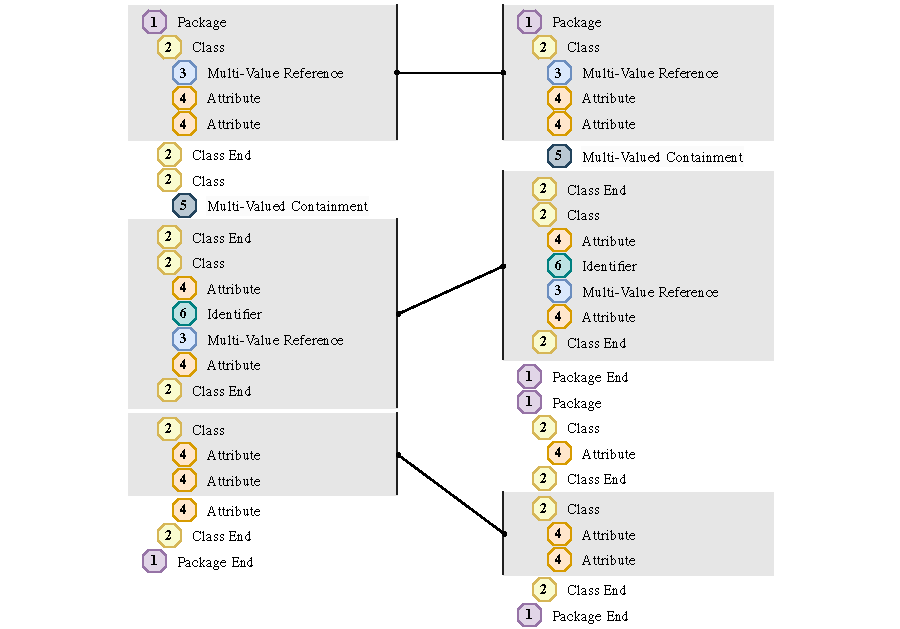
\includegraphics[width=\linewidth]{figures/mde/tokenMatching.pdf}
    \caption[Subsequence Matching for Modeling Artifacts]{Subsequence matches for the two token sequences of our running example in \autoref{fig:running-example} with a minimal token match of three. Three subsequences are matched with five, seven, and three tokens, respectively. The indentation solely serves illustrative purposes.}
    \label{fig:comparison}
\end{figure}

% ------------------------------------------------------------------
% 4. SIMILARITY CALCULATION
% ------------------------------------------------------------------

\section{Similarity Calculation}\label{subsec:similarity}

\noindent
The similarity calculation step remains unchanged when adapting token-based methods for detecting plagiarism in modeling assignments. Thus, we only briefly discuss this step.
As discussed in \autoref{sec:threatmodel-algebra}, the similarity of each modeling assignment pair can be calculated based on the subsequence matches.
For an assignment pair, the similarity can be calculated based on their token sequences with the symmetric similarity (\autoref{theo:avgsim}) or maximum similarity (\autoref{theo:maxsim}) metrics.
For pairs of assignments of different sizes, the maximum similarity can be used.
For pairs of assignments of different sizes, the maximum similarity is less resilient against false positives but better suited if many elements were inserted to obfuscate the plagiarism. We then use both metrics to rank pairs regarding their similarity. For our example in \autoref{fig:comparison}, the similarities are calculated to be $avgsim = 68.3\%$ and $maxsim = 71.4\%$, respectively.
%
Using these metrics, we can apply a wide variety of different post-processing to enhance the results for human inspection.
In practice, the following post-processing methods are commonly applied:
\begin{enumerate}[leftmargin=*]
    \item Ranked Lists of Pairs: A ranked list showing assignment pairs in descending order by similarity provides a prioritization for human inspection. Interactive refinements, such as filtering by similarity thresholds or excluding common template code, can streamline this process.
    \item Similarity Distribution: A histogram showing the distribution of similarity values for all comparisons, thus allowing us to identify what level of similarity is common for two given programs (probable true negatives) and what level of similarity indicates a comparison is an outlier (probable true positives).
    \item Clustering of Assignments: Using hierarchical agglomerative or spectral clustering to classify pairs according to their similarity helps detect group plagiarism.
    For the spectral clustering, automatic hyper-parameter search with Bayesian optimization using a Gaussian process as the surrogate model and L-BFGS for optimization \citet{Ng2001} can be employed. Configurable hyperparameters allow adaptation to different contexts, ensuring flexibility in analysis.
\end{enumerate}

These similarity metrics and post-processing techniques provide a robust foundation for educators to analyze the results of the plagiarism detection process. We ensure that individual and group plagiarism can be effectively identified via clustering analysis. This layered approach enhances detection quality and streamlines the subsequent human inspection process, making it more efficient in real-world educational settings.

% ------------------------------------------------------------------
% 5. VIZUALISATION
% ------------------------------------------------------------------

\section{Visualization}\label{subsec:visualization}


\noindent
An essential benefit of token-based approaches is the explainability of the calculated similarities. Moss~\cite{MOSS} and JPlag~\cite{prechelt2000}, for example, offer inspection of pairs of programs in a side-by-side code view, where the matched sections are highlighted. This facilitates the human assessment of the results and effective decision-making regarding what constitutes plagiarism. Providing this feature is crucial for the practical usage of plagiarism detectors \cite{Le2013}.
%
Graphical syntax and custom editors are commonly used to view and edit modeling artifacts. However, textual syntaxes benefit from linear structures that allow visualizing matches in a manner educators are used to from code plagiarism detectors. Nevertheless, a linear graphical syntax like a tree view also brings these benefits.

A suitable graphical or textual syntax has to be chosen for each modeling language. This makes this visualization step inherently domain-specific. This problem does not exist for code, as the persistent form of program code is the same form humans use to read and edit. For models, the persisted forms are rarely human-readable and do not reflect how they are viewed.

If a textual syntax is available, we propose using a side-by-side view based on textual syntaxes, thus effectively linearizing the modeling artifact.
The choice of textual syntax has to be domain-specific. For example, for \ac{EMF} metamodels, \textit{Emfatic}~\cite{Emfatic} allows us to depict them in a side-by-side view.
If no suitable textual syntax is available for a domain, a rudimentary solution is to implement a simple tree-based view based on the model elements and their tokenization references.

\begin{figure}
    \centering
    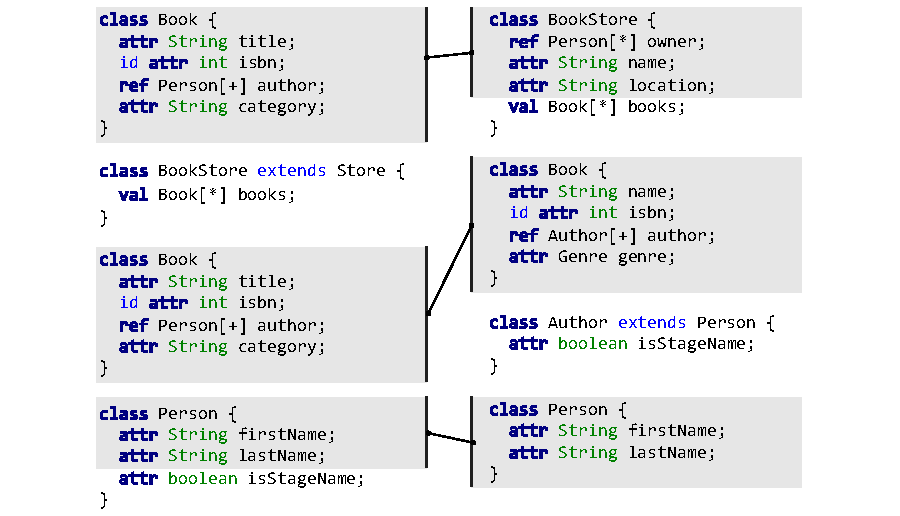
\includegraphics[width=\linewidth]{figures/mde/comparisonView.pdf}
    \caption[Visualization of Detected Modeling Plagiarism]{Textual representation of the matched metamodels fragments of our running example in \autoref{fig:running-example} via the Emfatic textual syntax~\cite{Emfatic}. This representation is similar to the typical visualization in source code plagiarism detection.}
    \label{fig:visualization}
\end{figure}

\autoref{fig:visualization} illustrates such a match visualization for the running example, which we calculated to be a 68.3 percent match. Emfatic is used to visualize the similarities between the metamodels. The three matches of \autoref{fig:comparison} are now traced back to the actual model elements. We observe that the class \texttt{Store} on the left side matches the class \texttt{BookStore} on the right side.
We also observe that the reference \texttt{books} on the right side is not matched, as it is part of the superclass \texttt{BookStore} on the left side. Furthermore, the classes called \texttt{Book} on both sides match despite different names and types of structural features. Finally, while both classes called \texttt{Person} match, the \texttt{isStageName} attribute is again moved into a superclass on the right side.
During human inspection, it is comprehensible how the similarity scores were calculated, and which parts are similar.
Even for such small models as depicted in \autoref{fig:running-example}, the side-by-side view in \autoref{fig:visualization} eases the comparison.


\section{Limitations}\label{sec:mde-limits}
In the following, we present two limitations of our approach.
First, we discuss the solution space problem, which is inherent to any plagiarism detection approach.
Second, we discuss the impact of the modeling domain and language on the effectiveness of our approach.

\subsection*{Domain-specific Tokenization}
As previously discussed, a generic tokenization strategy, which applies to a given model, will usually perform significantly worse for most models than a domain-specific one. Consequently, this makes finding a suitable mapping from model elements to tokens an inherently domain-specific problem. Thus, we cannot provide a universal solution for any given modeling domain or language. As an analogy, finding such a solution is like creating a universal model transformation that transforms between instances of any given metamodel. Any proposed solution would either be so broad that it lacks any purpose or would just not be universal.
While we provided a general framework and outlined the tokenization for the tokenization of \ac{EMF} models, it is up to the domain expert to find a suitable solution for a given modeling domain.
This limitation, however, is not unique to modeling languages, as existing literature does not provide detailed guidance for the tokenization of new programming language~\cite{Maertens2022, prechelt2002, prechelt2000, Joy1999}. Instead, examples are given for an exemplary programming language.

\subsection*{Wider Impact of the Modeling Domains}\label{sec:mde-limit-domain}
The effectiveness of our token-based plagiarism detection approach may vary depending on the modeling domain and language. It generally performs well for structural models and models where the semantic relationships form tree-based structures (e.g., containment trees). This covers most models used in \ac{MDE} education.
In some domains, however, models may represent highly abstract concepts with minimal structural detail, limiting the granularity available for tokenization. When structure is sparse or abstract, it becomes challenging to capture distinctive features that would reliably differentiate one model from another. This factor may especially play a role in behavioral models.

Further, the strength of semantic relationships (see \autoref{subsec:tokenization}), which our approach relies on to identify the semantic structure of the model, can vary greatly between domains. Some domains have well-defined, unambiguous semantic relationships that can be tokenized effectively, while for others, it is difficult to derive a consistent tokenization strategy. An example of such a case is \ac{UML} use case models. Here, it is nontrivial to find an order in which to linearize the models. Even though these models contain both relationships and associations, more empirical evidence is required to assess if, for example, actors should be considered before subsystems regarding the linearization order.

In sum, while our approach can be adapted to various modeling domains, the modeling domain's inherent characteristics affect how well our method performs. This limitation underlines the importance of customizing tokenization strategies to specific domains.

\subsection*{The Solutions Space Problem}
As discussed in \autoref{sec:mde-challenges}, detecting plagiarism in small modeling assignments can be challenging since these models require unique characteristics to distinguish them from others. Even minor structure, syntax, or modeling similarities can result in false positives. Furthermore, small modeling tasks often rely on commonly used patterns, making it difficult to differentiate between plagiarism and coincidental similarities, as the solution space of these assignments is minimal.
However, this limitation is inherent to plagiarism detection and thus also applies to code and natural language (see \autoref{sec:SPD-problem}). Consequently, whether manual checks or an automated approach like a plagiarism detector are employed, if the assignment size or complexity falls below a certain threshold, the space of all possible solutions collapses, and it is no longer possible to distinguish plagiarism cases from random similarities between unrelated solutions. This thus applies to our approach as it does to any other. However, this may occur more frequently in modeling assignments due to the challenge of abstraction Level and granularity (see \autoref{sec:mde-challenges}).
\chapter[Mitigating Obfuscation Attacks]{Mitigating Automated Obfuscation Attacks}\label{cha:defense}

As automated obfuscation attacks become increasingly sophisticated, robust defense mechanisms in software plagiarism detection systems are more vital than ever. In this chapter, we address this critical challenge by presenting defense mechanisms to enhance the resilience of these systems against various obfuscation strategies (\contribution{3}). All defense mechanisms discussed in the following apply to any token-based plagiarism detection system. As previously mentioned in \autoref{sec:SPD}, all state-of-the-art approaches used in practice fall into this category. Furthermore, the defense mechanism can also be applied to other structure-based detection approaches with little adaption needed.


The remainder of the chapter is structured as follows.
To effectively mitigate the risks posed by automated obfuscation, we first outline the specific requirements that defense mechanisms must meet.
%
The core of this chapter is dedicated to three novel defense mechanisms, each tailored to counter distinct types of obfuscation attacks:

\begin{description}
    \item[{Token Sequence Normalization}~\cite{Saglam2024b}] (see \autoref{sec:tsn}) utilizes specialized graphs to generate a normalized token sequence that is invariant to insertion- and reordering-based attacks. It combines the benefits of graph-based and token-based approaches by leveraging graph-based techniques to normalize the linear token sequence.

    \item[{Subsequence Merging}~\cite{Saglam2024c}] (see \autoref{sec:smm}) reverses obfuscation attacks by heuristically combining neighboring subsequences matches. Its attack-independent nature allows it to reverse the effects of a broad spectrum of obfuscation attacks, making it applicable to both programming and modeling assignments.

    \item[{Model Subtree Reordering}~\cite{Saglam2024a}] (see \autoref{sec:msr}) is specifically designed for modeling artifacts, such as \ac{EMF} metamodels or \ac{UML} models. The mechanism employs a multi-step algorithm that normalizes the order of nodes in the model tree, effectively countering reordering attacks.
\end{description}

In addition to these primary mechanisms, the chapter also explores other, less effective defense strategies. While these alternative approaches offer some protection, they have notable downsides or are less effective than our primary defense mechanisms.


\ownpublications{
\fancycite{Saglam2024b},
\fancycite{Saglam2024a},\\
\fancycite{Saglam2024d}, and
\fancycite{Saglam2024c}.
}

\section{Requirements}\label{sec:tsn-requirements}
Before we discuss our different defense mechanisms against obfuscation attacks, we want to highlight the key requirements for such mechanisms.
These requirements are directly derived from the obfuscation attack threat model introduced in \autoref{cha:threatmodel}.
%
In addition to these imperative requirements, language dependence is an important factor to discuss, as it greatly affects the applicability of any given defense mechanism.

For any normalization approach to be applicable in real-world scenarios, it must meet the following requirements.
Firstly, it must operate at an {abstract level}, focusing on tokens rather than code.
Furthermore, it must support {explainability}~\cite{Karnalim2021} via traceability between input programs and the computed matches and similarity scores, allowing for the visualization of potential plagiarism with the original, {unaltered program}.
The fact that it is unaltered is essential from both ethical and administrative perspectives~\cite{Simon2016}, as it ensures that the original code remains the basis for human decision-making in plagiarism detection~\cite{Le2013}.
Furthermore, the altered code may no longer contain \textit{idiosyncrasies} (e.g., obvious obfuscation attempts) that assist the decision-making~\cite{Novak2019}.
Consequently, normalization approaches that modify the input programs as pre-processing steps are not applicable.
Existing code normalization approaches, such as dead code elimination with program dependence graphs, do not meet these requirements.

\begin{description}
    \item[Language-Dependence] Implementing a defense mechanism as a pre-processing step for the input programs is language-specific, necessitating a newly designed mechanism for each supported language. This is tedious and costly, and thus, a defense mechanism should be \textit{language-independent}, ensuring versatility across programming languages. However, the more language-independent an approach is, the more abstract the information on which it operates. This abstraction provides a challenge that needs to be addressed to avoid affecting the effectiveness of the defense mechanism. At a minimum, the approaches should be \textit{language-agnostic}, meaning they require some adaption for each language but do not require a complete redesign.
    %Our approach is language-independent, ensuring versatility across languages.
    
    \item[Abstraction Level] For seamless integration into token-based approaches, any defense mechanism must operate at an abstract level, focusing on tokens rather than code, enabling the capture of structural similarities while minimizing the influence of language-specific syntax~\cite{prechelt2002, liu2006, Nichols2019}. 
    %
    This abstraction allows the defense mechanism to generalize across different programming languages, making it versatile and broadly applicable. By focusing on the structural patterns of the code rather than its specific syntax, the mechanism operates on the same level as the detector. This avoids depending on vulnerable information, e.g., variable names or types, that can be used as an additional attack vector.

    \item[Explainability] Any defense mechanism must preserve explainability~\cite{Karnalim2021}, meaning there should always be the ability to understand the similarity score, how it was computed, and which parts of the input programs are similar or dissimilar. This requirement is crucial for maintaining transparency and ensuring educators and other stakeholders trust the detection process. This includes providing clear insights into the matching process and highlighting the code fragments contributing to the final similarity score. In many countries, academic misconduct investigations are led by administrative staff~\cite{Simon2016}. In these cases, explainability is especially critical.

    \item[Preserving Originality] In plagiarism detection, plagiarism detectors must deliver evidence based on the input programs. 
    It becomes difficult to convince non-expert staff when using altered programs as the basis of an argument~\cite{Le2013}. Accused individuals may rightfully assert that the altered programs are not what they originally submitted, thus hindering explainability.
    Moreover, when using pre-processed or altered programs for result visualization, the programs might seem more similar to the human observer than they were initially.
    Thus, the original, unaltered code must be used for human decision-making~\cite{Le2013}.
    Ideally, the subsequence matching and similarity calculation is resilient to obfuscation attacks, but the original, unaltered code is used to visualize these results.
    
    \item[Preserving Idiosyncrasies] Similarly, when the altered code is used for the visualization, some idiosyncrasies of the original programs (e.g., obvious obfuscation attempts) are no longer present. However, these idiosyncrasies are often used as evidence for both initial decision-making and presentation of evidence in misconduct investigations and the related hearing with the students~\cite{Novak2019, Denzler2024}. Hence, relying on altered code renders presenting a compelling argument in a plagiarism case considerably more challenging. It thus negatively affects human decision-making.
    
    \item[Automation] In software plagiarism detection, the similarity calculation must be fully automated to effectively tackle the problem at scale. A defense mechanism that breaks this property and requires human intervention during the pairwise comparison becomes inapplicable at scale. Automation ensures that the defense mechanism can handle the data of large courses efficiently. Human decision-making should only begin once the results are presented, allowing for scalable and efficient plagiarism detection.
     
\end{description}


\section{Token Sequence Normalization}\label{sec:tsn}

In this section, we introduce our first defense mechanism (\contribution{3.1}) called \textit{token sequence normalization}~\cite{Saglam2024b}.
A few years ago, \citet{DevoreMcDonald2020} introduced \textit{\mossad}, a plagiarism generator inspired by genetic programming that allows generating multiple obfuscated versions of a single program.
While most software plagiarism detectors exhibit resilience against some \textit{obfuscation attacks}~\cite{Joy1999,prechelt2000}, \mossad exploits a vulnerability that is inherent in the most widely used approaches.
Although there are graph-based approaches that are potentially less vulnerable to such attacks, they are not feasible in practice~\cite{liu2006} since the subgraph isomorphism problem is NP-complete~\cite{Shang2008, McCreesh2020, Lubiw1981}.

As discussed, \mossad repeatedly inserts statements into the plagiarized program to interfere with the subsequence matching of a potential detector.
To that end, sets of pre-defined statements called \textit{entropy} and existing statements from the original program are used.
The insertion is stopped when the plagiarized instance falls below a certain similarity threshold compared to the original.
%
While \mossad is only one example of an automated obfuscation attack, it is highly effective as similar attacks based on statement insertion are not hard to implement. Thus, it is especially important to provide strong resilience to insertion-based obfuscation.

Token sequence normalization successfully provides resilience against such automatic obfuscation attacks.
It combines the effectiveness of graph-based approaches with the scalability of token-based approaches in a best-of-both-worlds approach\footnote{Subgraph isomorphism for two graphs with $n$ vertices has a runtime complexity of $O(n^n)$. Moreover, the advantage of token sequence normalization is that it has to be performed once per program, not per comparison.}.
We leverage program dependence graphs (PDG)~\cite{ferrante1987} to normalize programs.
However, for real-world applicability, any approach should not be language dependent and operate at an abstract level~\cite{prechelt2002, liu2006, Nichols2019}. Furthermore, it must support explainability via traceability, enabling visualization based on the original, unaltered code.
From both ethical and administrative standpoints~\cite{Simon2016, Le2013}, only the original, unaltered code should inform human decision-making in academic misconduct investigations.
Moreover, the unaltered code often contains idiosyncrasies~\cite{Novak2019} due to obfuscation. They are used for both initial decision-making and misconduct investigations.
Hence, it is not sufficient to eliminate dead code in the input programs.
Existing dead code elimination methods do not fulfill these requirements, as they are fully language-dependent, modify the programs, and are incompatible with ethical and administrative concerns.

In contrast to dead code elimination, our defense mechanism is specifically designed to meet these requirements.
It expands upon the inherent resilience of token-based approaches by making the token sequence virtually invariant against insertion- and reordering-based attacks.
As part of that, we introduce the concept of a \textit{token normalization graph} (TNG), which operates on the token sequence and is thus language-independent.
With that token normalization graph, we normalize the token sequence by removing dead statements and putting subsequent independent statements in a fixed order.
Thus, we effectively reverse the insertion and reordering of statements and de-obfuscate plagiarism instances, thereby achieving high resilience to automatic plagiarism based on these attacks.

\begin{factsheet}{Overview: Token Sequence Normalization} 
    \begin{description}[style=multiline,leftmargin=5.5cm]
        \item[Core Principle] Normalize Token Sequence \\via Graph-Based Representation
        \item[Targeted Obfuscation Attack] Statement Insertion, Statement Reordering
        \item[Language Family] Programming Languages
        \item[Language Dependence] Language-Agnostic
        \item[Performance Impact] Low
        \item[Main Scalability Determinant] Size of Input Programs 
        \item[Integration Complexity] Moderate
    \end{description}
\end{factsheet}

\subsection{Targeted Obfuscation Attacks} \label{sec:icseb:RunningExample}

Token sequence normalization is designed to defend against two particular obfuscation attack types: Semantic-preserving statement insertion and statement reordering. These attacks aim to affect the token sequence derived from a program by modifying the program without changing its underlying behavior, thereby misleading plagiarism detection tools. %Two primary forms of targeted obfuscation attacks are considered: reordering of independent statements and insertion of (dead) statements.

%\subsubsection{Insertion of (Dead) Statements}
A simple yet effective obfuscation attack is the insertion of dead statements. Dead statements are lines of code that do not affect the program's output or behavior. These can include redundant assignments, unused variables, or code blocks that are never executed (e.g., due to always-false conditions). An attacker can significantly alter the token sequence without changing the program's functionality by inserting such statements at various points in the code. Furthermore, dead statements can be obfuscated themselves by inserting further statements that depend on them.

\begin{samepage}
\begin{lstlisting}[caption={Example for Obfuscated Dead Statements},label=lst:complexinsertion]
int x = 10;
boolean checked = false; // Dead statement
int y = 5;
if (checked) { // Dead block, only depends on the dead statement
    y = 20;
}
println(x + y);
\end{lstlisting}
\end{samepage}

\autoref{lst:complexinsertion} illustrates such a dependence between inserted statements. Both the variable \texttt{checked} and the control structure are dead code. However, the variable is referenced as a condition of the control structure.
However, as these statements do not alter the behavior of the program, they are still dead code. However, it is harder to detect them, as statement interdependence has to be fully resolved.

%\subsubsection{Reordering of Independent Statements}
Reordering independent statements involves changing the order of code statements that do not depend on each other, meaning the order of the statements does not affect the behavior of the program. This type of obfuscation leverages the fact that most programming languages allow statements that do not affect each other's execution order to be rearranged. For example, swapping the order of two variable assignments that do not depend on each other's values is possible. This attack is considered a weak form of obfuscation, as the degree of freedom to reorder statements in most programs is limited. Only some statements can be reordered, thus making it challenging to apply this obfuscation broadly.

Both statement insertion and reordering can be automated in different ways. Our defense mechanism is designed to counter these attacks independent of their automation, be it \mossad-style random obfuscation until a certain threshold is reached or exhaustive obfuscation where the obfuscation is applied to all possible code positions.

\noindent
As a combined running example for both insertion and reordering, we introduce the programs shown in \autoref{tab:codesnippet}. 
Both programs print the squared values of the numbers from 1 to 10.
The right program is a modified variant based on two changes that alter its structure.
Thus, the program still behaves the same upon execution.
In detail, line 3 was inserted in the modified variant, and lines 6 and 7 were swapped.
%Minimal example, no focus on renaming as popular code plagiarism detectors are resilient by using abstraction \cite{} 
%Also, there is no focus on deletion, as it is not practical if functionality should not be reduced
While the relationship between the programs is evident in this simple example, this is not true for larger programs that undergo extensive modifications to obfuscate the relation between the variant and the original. Thus, these modifications can be used to conceal plagiarism. 
Additionally, manual comparison becomes infeasible when dealing with numerous student submissions, even for smaller programs.
However, for plagiarism detectors, structural obfuscation attacks like these diminish the detection quality~\cite{DevoreMcDonald2020}. 
%Easy to detect, but only minimal example. Large-scale obfuscation in thousands of lines with hundreds of submissions, easy to be overlooked

To illustrate this, \autoref{tab:tokens} shows the token sequences of the two programs in \autoref{tab:codesnippet}.
While the structural information concerning method context, loop context, declarations, and assignments remains intact, specific details such as names, types, or comments are excluded.
Note that the changes lead to two sequences that are different enough to affect the detection quality, as only shorter subsequences can be matched between them. In detail, we can find three matching subsequences of length two: The first two lines, the last two lines, and finally, lines four and five. As discussed, these subsequences are short enough to fall below the plagiarism detector's threshold.

\begin{samepage}
\begin{table}
	\centering
	\begin{tabular}{rlcl}
		\toprule
		\textbf{\#} & \textbf{Original}                              &                  & \textbf{Variant}                                   \\
		\midrule
		1           & \texttt{~~void printSquares() \{}              &                                    & \texttt{~~void printSquares() \{}                  \\
		2           & \texttt{~~~~int i = 1;}                        &                                    & \texttt{~~~~int i = 1;}                            \\
				
		3           &                                                & \small\textbf{\phantom{$\to$}  insert $\to$} & \cellcolor{add}\texttt{~~~~boolean debug = false;} \\
				
		4           & \texttt{~~~~while (i <= 10) \{}                &                                    & \texttt{~~~~while (i <= 10) \{}                    \\
		5           & \texttt{~~~~~~int square = i * i;}             &                                    & \texttt{~~~~~~int square = i * i;}                 \\
		6           & \cellcolor{del}\texttt{~~~~~~println(square);} & \small\textbf{$\to$ reorder $\to$} & \cellcolor{add} \texttt{~~~~~~i++;}                \\
		7           & \cellcolor{del}\texttt{~~~~~~i++;}             & \small\textbf{$\to$ reorder $\to$} & \cellcolor{add} \texttt{~~~~~~println(square);}    \\
		8           & \texttt{~~~~\}}                                &                                    & \texttt{~~~~\}}                                    \\
		9           & \texttt{~~\}}                                  &                                    & \texttt{~~\}}                                      \\
		\bottomrule
	\end{tabular}
    \caption[Example Obfuscation: Insertion and Reordering]{Original code (left) and modified variant (right) after inserting one statement and reordering two. Removed lines are highlighted in red, and added lines are highlighted in green.}
	\label{tab:codesnippet}
\end{table}


\begin{table}
    \centering
    %\small
    \begin{tabular}{c@{\hskip 15pt}l@{\hskip 30pt}c@{\hskip 30pt} r}
        \toprule
        \# & \textbf{Original Tokens}     &                     & \textbf{Variant Tokens}      \\
        \midrule
        1  & \texttt{method start} &                 & \texttt{method start} \\
        2  & \texttt{variable}     &                 & \texttt{variable}     \\
        3  &                       & \textbf{\phantom{$\to$}  insert $\to$}    & \cellcolor{add}\texttt{variable}     \\
        4  & \texttt{loop start}   &                 & \texttt{loop start}   \\
        5  & \texttt{variable}     &                 & \texttt{variable}     \\
        6  & \cellcolor{del}\texttt{apply}        & \textbf{$\to$  swap $\to$} & \cellcolor{add}\texttt{assignment}   \\
        7  & \cellcolor{del}\texttt{assignment}   & \textbf{$\to$  swap $\to$} & \cellcolor{add}\texttt{apply}        \\
        8  & \texttt{loop end}     &                 & \texttt{loop end}     \\
        9  & \texttt{method end}   &                 & \texttt{method end}   \\
        \bottomrule
    \end{tabular}
    \caption[Example Obfuscation Tokens: Insertion and Reordering]{Comparison of the original and obfuscated token sequences corresponding to the program statements in \autoref{tab:codesnippet}. One token is inserted at index 3, while two tokens at indices 6 and 7 are swapped.}
    \label{tab:tokens}
\end{table}
\end{samepage}

\subsection{Concept}

The defense mechanism is an additional step in the pipeline of a plagiarism detector before the pairwise comparison, which effectively de-obfuscates plagiarism for the remaining steps in the pipeline.
At a high level, our mechanism operates as follows for each input program:

\begin{enumerate}
    \item We enrich the token sequence with additional language-agnostic semantic information about the interdependence of the tokens.
    \item We construct a language-independent graph-based representation of the tokenized program from the enriched token sequence, which abstracts from the original code. This graph represents a partial order of the tokens.
    \item We then use this graph to generate a normalized token sequence, thus effectively reverting insertions and reordering operations.
    \begin{enumerate}
        \item Insertions are countered via subsequence removal.
        \item Reordering is negated by topological sorting~\cite{kahn1962}.
    \end{enumerate}
    \item The comparison is still conducted exclusively on the token sequence, circumventing the computational complexity of graph-based approaches.
\end{enumerate}

\noindent
We call the representation of the tokenized program a \textit{token normalization graph} (TNG).
Each node in this graph represents the tokens of a program statement.
As it is based on the token sequence, it is language-independent, which enables our defense mechanism to be applicable to any programming language.
Thus, the format of the semantic information utilized to enrich the token sequence must also be language-independent.
%
We specify a generic format for the semantic information based on the interdependence between tokens that abstracts from the detail of the underlying programming language.
The semantic information must be extracted from the input programs alongside the tokens.
Therefore, the extraction needs to be implemented separately for each language the detector supports.
It is the sole language-dependent step that our defense mechanism adds.
While the format of the semantic information and the TNG is language-independent, the need to provide this information makes the defense mechanism language-agnostic.
However, extracting semantic information does not impose additional constraints on the detector since tokenization is inherently language-dependent.


\subsection{Semantic Information}

\label{subsec:semantic}
In order to construct a TNG, we need information about the interdependencies between the tokens.
This information is not present in the token sequence and thus must be additionally attached to the tokens.
To that end, a language-independent format is required for this semantic information.
Using this format, the tokens can be automatically annotated during their extraction from the parse tree. Different types of statements lead to different types of information.
Thus, this format allows us to map the relations of the statements in the program to the tokens independent of the underlying language of the program.
%
We specify the following format for this semantic information:
%\begin{samepage}
\begin{description}
    \item[Criticality] describes statements that contribute to programs' behavior through means other than variables and thus must not be removed. Therefore, a token can be either critical or not critical.
        \textit{In our example in \autoref{tab:codesnippet}, the critical statements are the \texttt{while} statement and the \texttt{println} statement. Thus, the \texttt{loop start} and \texttt{apply} tokens in \autoref{tab:tokens} are critical.}
    \item[Fixed Order] describes how statements must maintain their relative order to ensure semantic equivalence. Tokens can thus be either fixed in their order or non-fixed. Fixed order tokens act as reordering boundary, as preceding tokens cannot be moved after this boundary and vice versa.
        \textit{In the running example, the \texttt{while} statement dictates that the statements within the loop cannot be moved outside the loop. Thus, the loop tokens of lines 4 and 8 in \autoref{tab:tokens} are fixed order tokens.}
    \item[Variable Access] describes the variable accesses (read or write) for each statement, thus indicating on which other statements they depend.
        Hence, each token has two variable identifier sets: One for read accesses and one for write accesses.
        \textit{In the running example, the \texttt{while} statement depends on the statement the declares the variable \texttt{i}. Therefore, the \texttt{loop start} token contains \texttt{i} in its read access set.}
    \item[Loop] describes statement blocks in which the execution order of the statements can deviate from their declaration order. Therefore, the first and last tokens corresponding to the loop are marked with loop start and loop end flags.
        \textit{In the running example, the statements in the loop body are repeatedly executed. Thus, the incrementation of the variable \texttt{i} may be executed not only after the \texttt{println} statement but also before due to the repeated execution. In the running example, both \texttt{loop start} and \texttt{loop end} are marked with the loop flag.}
\end{description}
%\end{samepage}


\subsection{Token Normalization Graph}

We use the token normalization graph (TNG) as the underlying data structure to generate a normalized token sequence.
A TNG is a specialized version of a program dependence graph (PDG).
It is designed for tokens instead of code and through a higher abstraction level not confined to the programming language's syntax. Thus, a TNG crucially provides language independence. A TNG contains additional edges required for the token sequence normalization.
While a PDG focuses only on statement dependencies in code, the TNG considers both token interdependence and the order of the tokens. Both are required for token-based approaches.

We construct the TNG from the token sequence and the additional semantic information.
A TNG node represents a single statement and contains all tokens generated from that statement.
After the construction of the TNG, we no longer need the original token sequence.
%
More formally, a token normalization graph is a directed graph \( G = (V, E) \) used to represent the tokenized form of a program for the purpose of normalization. Each node \( v \in V \) represents a statement in the program and contains a subsequence of tokens. Let \( (t_i) \) be the sequence of all tokens in the program. Each statement \( S \) corresponds to a subsequence \( (s_j) \sqsubseteq (t_i) \) where \( (s_j) \) is the set of tokens extracted for \( S \). Thus, each node in the TNG is represented by a subsequence of tokens.
%
The TNG has three types of directed edges, each capturing different dependencies between the statements represented by the nodes:
\begin{description}
    \item[Variable Flow Edges] indicate that a statement writes to a variable that another statement reads. They are similar to the data dependencies in the PDG.
    \textit{A directed edge \( (v_i, v_j) \in E \) is a variable flow edge $(v_i, v_j) \in E_{vf}$ if statement \( S_i \) of $v_i$ writes to a variable that statement \( S_j \) of $v_j$  reads. This edge indicates a data dependency where \( v_j \) depends on \( v_i \) for the value of the variable.}
    
    \item[Variable Order Edges] indicate that altering the order of the two statements may alter variable values and, thus, the program's behavior.
    This edge helps maintain the correct execution order of statements.
    Wherever there is a variable flow edge, there is also a variable order edge; however, not necessarily in the same direction.
     \textit{A directed edge \( (v_i, v_j) \in E \) is a variable order edge $(v_i, v_j) \in E_{vo}$ if changing the relative order of statements \( S_i \) and \( S_j \) could alter the program's behavior due to variable dependencies.}
     
    \item[Fixed Order Edges] indicate that altering the order of the two statements may affect the program's behavior for reasons beyond variable value alterations.
    This edge enforces the preservation of the original order of critical statements.
    \textit{A directed edge \( (v_i, v_j) \in E \) is a fixed order edge $(v_i, v_j) \in E_{fo}$ if changing the order of statements \( S_i \) and \( S_j \) could affect the program's behavior for reasons other than variable dependencies.}   
\end{description}

\noindent
The TNG is then constructed as follows:
First, we group all tokens within a statement as nodes. %, and edges are then formed based on the tokens' semantic information.
For each statement \( S \) in the program, create a node \( v_i \) containing the subsequence of tokens \( (s_j) \sqsubseteq (t_i) \).
Next, we label nodes containing at least one critical token as \textit{critical}.
We then use the tokens marked as \textit{fixed order} to create fixed order edges $E_{fo}$.
For each node with fixed order tokens, we create incoming and outgoing edges to and from all preceding and subsequent nodes, as determined by the original order of the tokens.
We employ the variable access sets and loop flags to create variable flow edges $E_{vf}$.
Finally, disregarding loop flags, we determine variable order edges $E_{vo}$ solely by variable access sets.
Once the TNG is complete, it contains all the necessary data for generating a normalized token sequence. Thus, the original token sequences can be safely discarded.
Moreover, as for all token-based approaches, the original programs are no longer required for the similarity calculation.


\begin{figure}
\centering
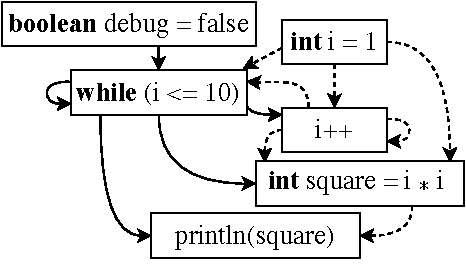
\includegraphics[width=0.5\linewidth]{figures/pdg.pdf}
\caption[Program Dependence Graph]{Program dependence graph of the running example showing control dependencies (solid arrows) and data dependencies (dashed arrows).}
\label{fig:pdg}
\end{figure}


\autoref{fig:pdg} shows a PDG for the plagiarized program in \autoref{tab:codesnippet}. The control and data dependencies between the different code statements are represented via edges.
While the dead statement for the variable called \texttt{debug} can be identified, it cannot be used to generate a normalized token sequence due to the requirements mentioned in \autoref{sec:tsn-requirements}.
\autoref{fig:tng} shows the TNG for the same program. In contrast to the PDG, the nodes represent tokens instead of code. The TNG contains the three types of edges based on the semantic information discussed in \autoref{subsec:semantic}. The two nodes with a gray background are marked as critical. Furthermore, the semantic information of the corresponding tokens is illustrated in the bottom right corner of the node. 
The semantic information is only depicted for the sake of clarity. It is used to construct the TNG but is no longer necessary for the normalization thereafter.

\begin{figure}
\centering
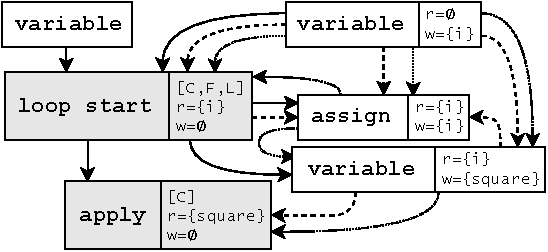
\includegraphics[width=0.6\linewidth]{figures/tng3.pdf}
\caption[Token Normalization Graph]{Token normalization graph for the PDG in \autoref{fig:pdg}, fixed order edges (solid), variable order edges (dashed), and variable flow edges (dotted).
The critical (C), fixed-order (F), and loop (L) flags, with the variable access sets (r for read, w for write), are included for illustrative purposes.}
\label{fig:tng}
\end{figure}


\subsection{Generating the Normalized Token Sequence}

After constructing the TNG, we can leverage it to generate a normalized token sequence in two steps.
%We do so in two steps: One for reverting insertions and one for reverting reordering.
First, we remove all dead nodes. These are all nodes from which no critical node can be reached via variable flow edges $E_{vf}$. This effectively reverts insertions into the token sequence.
Next, we remove all variable flow edges $E_{vf}$ from the TNG, making it acyclical. They have served their purpose for the dead node removal and are no longer required.
In our running example in \autoref{tab:codesnippet}, the statement containing the variable named \texttt{debug} is considered dead code, and so is its corresponding \texttt{variable} node in the TNG in \autoref{fig:tng}.
This node will be removed, as it has no outgoing variable flow edge.
\autoref{tab:tokens-full} illustrates how that affects the normalized token sequence. The code insertion leads to an additional token in the obfuscated token sequence. However, after the dead node removal, this effect is reversed.
\autoref{fig:tng2} illustrates the TNG from \autoref{fig:tng} with the dead node removed and variable flow edges $E_{vf}$ omitted. The previous cycles, such as the one between the \texttt{loop start} and \texttt{assign} nodes, are no longer present.
A partial order becomes apparent when considering the topmost \texttt{variable} node as the root.

\begin{figure}[b]
\centering
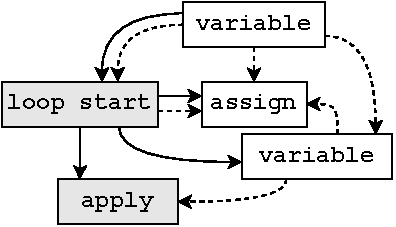
\includegraphics[width=0.45\linewidth]{figures/tng2b.pdf}
\caption[Reduced Token Normalization Graph]{Token normalization graph after the dead nodes and removal of variable flow edges, still present are fixed order edges (solid) and variable order edges (dashed).}
\label{fig:tng2}
\end{figure}

Next, we use topological sorting~\cite{kahn1962} to generate a normalized token sequence. This counters attempts to reorder the token sequence.
Specifically, we order the tokens of the remaining nodes by their node's distance to the aforementioned root.
Nodes with the same distance represent subsequent independent statements. We sort them via the types of tokens in the nodes.
This is a robust criterion, as the extracted tokens are invariant to lexical modifications~\cite{prechelt2002}.
Note that if two nodes with the same root distance are equal according to that criterion, they contain the same tokens, and their order does not affect the normalized token sequence. %; therefore, we can consider them equal in order.

In our running example in \autoref{tab:codesnippet}, statements 6 and 7 were swapped.
\autoref{tab:tokens-full} illustrates how this obfuscation affects the token sequence.
When using the reduced TNG in \autoref{fig:tng2} to generate the normalized token sequence, the sequence after the topological sorting will be identical to the original one (see \autoref{tab:tokens-full}). Thus, the plagiarism detector computes a 100\% match for our running example, despite the obfuscation attempt shown in \autoref{tab:codesnippet}.
Our approach only normalizes the tokens sequence. The original, unaltered code, with all its idiosyncrasies, is used for the visualization. However, as a result of our normalization, the similarity calculation and code matching are not compromised by obfuscation attacks.




\begin{table}
    \centering
    \begin{tabular}{c@{\hskip 12pt}c@{\hskip 4pt}c@{\hskip 4pt}c@{\hskip 4pt}c@{\hskip 4pt}c@{\hskip 4pt}c@{\hskip 4pt}c}
        \toprule
        \# & \textbf{Original} & $\to$ & \textbf{Obfuscated} & $\to$ & \textbf{Nodes Removed} & $\to$ & \textbf{Top. Sorted} \\
        \midrule
        {1}  & \texttt{method start} & & \texttt{method start} & & \texttt{method start} & & \texttt{method start} \\
        {2}  & \texttt{variable}     & & \texttt{variable}     & & \texttt{variable}     & & \texttt{variable}     \\
        {3}  &                                  & \textbf{(+)} & \texttt{\textbf{variable}}     & \textbf{(--)} & & &  \\
        {4}  & \texttt{loop start}   & & \texttt{loop start}   & & \texttt{loop start}   & & \texttt{loop start}   \\
        {5}  & \texttt{variable}     & & \texttt{variable}     & & \texttt{variable}     & & \texttt{variable}     \\
        {6}  & \texttt{apply}        & \textbf{(\textasciitilde)} & \texttt{\textbf{assignment}}   & & \texttt{\textbf{assignment}}   & \textbf{(\textasciitilde)}& \texttt{apply}   \\
        {7}  & \texttt{assignment}   & \textbf{(\textasciitilde)} & \texttt{\textbf{apply}}        & & \texttt{\textbf{apply}}        & \textbf{(\textasciitilde)}& \texttt{assignment}        \\
        {8}  & \texttt{loop end}     & & \texttt{loop end}     & & \texttt{loop end}     & & \texttt{loop end}     \\
        {9}  & \texttt{method end}   & & \texttt{method end}   & & \texttt{method end}   & & \texttt{method end}   \\
        \bottomrule
    \end{tabular}
    \caption[Token Sequence Normalization]{Comparison of the original and obfuscated token sequences with the obfuscated one after the two steps dead node removal and topological sorting \autoref{tab:codesnippet}.}
    \label{tab:tokens-full}
\end{table}


\subsection{Complexity}

The runtime complexity of token sequence normalization depends on extracting the semantic information, creating the token normalization graph, and generating the normalized token sequence.
The semantic information can be extracted during the tokenization step of the plagiarism detector and does not occur at an additional cost.

For the other steps, the runtime complexity depends on the density of the graph and, thus, on its number of nodes, which is limited by the number of tokens $m$ and its number of edges $e$.
As for a PDG, building a TNG can take $O(m^2)$ time in the worst case due to dense dependencies among tokens.
Pruning dead nodes requires a reachability analysis using a graph traversal with a $O(m + e)$ complexity. Topological sorting is performed on the resulting TNG and takes $O(m + e)$ time.

Therefore, the overall runtime complexity is $O(m^2)$ in the worst case (for dense graphs) and $O(m + e)$ in the best case (for sparse graphs).
Note that this has to be done for every input program but not for every comparison, which is a strong advantage compared to graph-based plagiarism detection methods. Thus, doing so for $n$ programs of maximum $m$ tokens has a worst-case complexity of only $O(nm^2)$. Thus, the size of the input programs has a larger impact on the performance of the token sequence normalization than the number of programs.
%
As the worst-case runtime complexity for greedy string tiling for $n$ programs with $m$ tokens, each is \( O(n^2m^3) \) (see \autoref{sec:found-jplag}), token sequence normalization does not increase the runtime complexity of the plagiarism detection process.


\subsection{Observed Impact}
This section presents initial observations on the effectiveness of token sequence normalization based on real-world data. It is important to note that this is not intended as a comprehensive evaluation but instead aims to provide an empirical perspective on how the defense mechanism performs in practical scenarios.

When applying token sequence normalization in practice, we can observe that it effectively renders obfuscation attacks based on insertion and reordering ineffective.
Remarkably, the similarity of unrelated solutions remains virtually unaltered, with an average similarity increase of less than 1\%, effectively avoiding an increase in false positives.
Our defense mechanism comes with a negligible runtime overhead of mere seconds for large real-world datasets, thus showing its practicality.

\autoref{fig:tsn-impact} illustrated the effectiveness of our approach in preventing obfuscation statement insertion.
The solid lines show how the similarity computed by JPlag decreases the more statements proportionally to the input program size are inserted.
Without our defense mechanism, the similarity values drop below 10\%. This renders successful plagiarism detection ineffective, as plagiarized programs can no longer be distinguished from original ones.
To achieve such a low threshold, approximately 50-60\% additional statements need to be inserted.
Note that we employed PlagGen~\cite{Broedel2023} for the obfuscation, which uses an exhaustive strategy. Thus, the input program determines how many statements can be inserted. 

The dashed lines show the same input programs but with token sequence normalization enabled. 
There, the similarity values surge to over 99\%. These results would raise strong suspicions, as for its dataset, the average similarity of unrelated programs is around 10\%. Thus, token sequence normalization renders the obfuscation attack ineffective, making the detector resilient against these attacks.

\begin{figure}[ht]
    \centering
    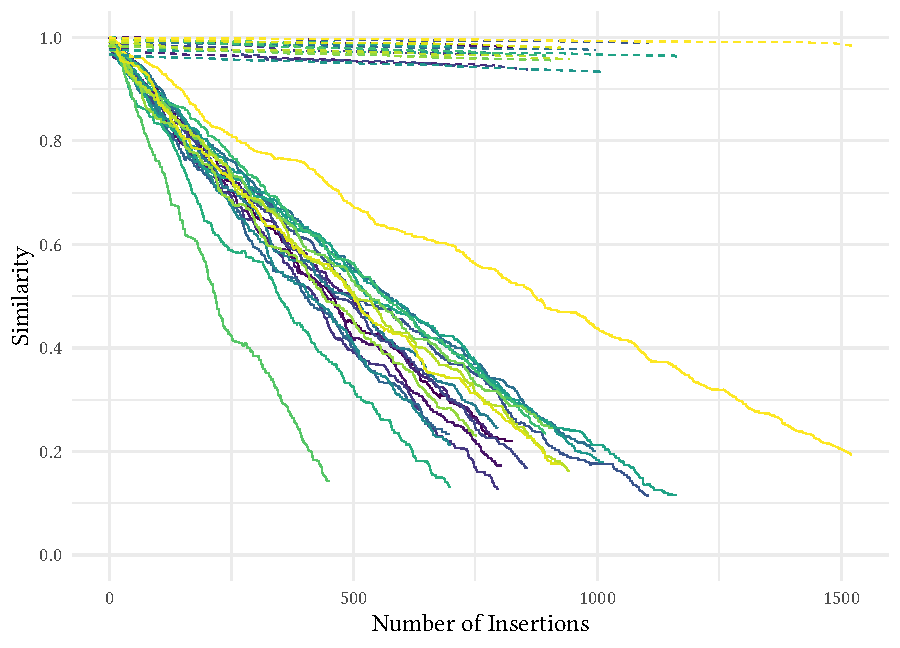
\includegraphics[width=1\linewidth]{figures/eval-tsn-steps.pdf}
    \caption[Impact of Token Sequence Normalization]{Similarities calculated by JPlag for obfuscated programs of a real-world introductory programming assignment dataset with an average of 1529 lines of code (LOC) per program via step-wise statement insertion as obfuscation attack. Each line represents a program, solid lines for JPlag as the baseline, and dashed lines are for JPlag with token sequence normalization.}
    \label{fig:tsn-impact}
\end{figure}

To assess the performance implications of our mechanism, we compared the runtime of JPlag with and without our approach.
We measured the runtime for two real-world datasets. We employed a consumer notebook, specifically a MacBook Pro equipped with an M1 Pro chip and 16GB of memory, for our performance measurements to provide a realistic environment.
As shown in \autoref{fig:tsn-runtime}, there is only an overhead of 0.89 seconds for one dataset and 6.45 seconds for the other. Note that this is the overhead for the complete datasets, not individual programs. State-of-the-art software plagiarism detectors like JPlag are highly optimized, and the performance impact of our mechanism is negligible. Thus, the total runtime of JPlag combined with our mechanism is mere seconds.

    \begin{table}
	\centering
	\begin{tabular}{llrrr}
		\toprule
		  Dataset Name & Metric     & JPlag     & JPlag with TSN & Difference\\
		\midrule
		\multirow{ 2}{*}{TicTacToe} & Runtime    & 6.97s     &    7.86s   & +0.89s\\
        %         &Relative Runtime   & 100.0\% &    112.7\% &\\ % with exact measurements it's . 7
	               &  $\sigma$ (SD)    & 0.10s     &    0.10s &+0.00s\\
        \hline 
        \multirow{ 2}{*}{BoardGame}   & Runtime          & 16.83s     &    23.28s   & +6.45s\\
		              & $\sigma$ (SD)    & 0.53s      &    0.44s    & -0.09s \\
		\bottomrule
    \end{tabular}
    \caption[Runtime Overhead of Token Sequence Normalization]{Runtime overhead of JPlag with token sequence normalization for two introductory programming assignment dataset TicTacToe (626 programs, 167.562 LOC total, \textasciitilde200.000 comparisons) and BoardGame (434 programs, 685.730 LOC total, \textasciitilde94.000 comparisons), avg. of 100 runs.}
	\label{fig:tsn-runtime}
    \end{table}
    

\subsection{Limitations}\label{sec:tsn-limits}

While token sequence normalization is a highly effective defense mechanism against insertion-based obfuscation attacks, it does have certain limitations. In the following, we discuss its dependence on the quality of the extracted semantic information and its applicability to other programming paradigms.

\subsubsection{Dependence on Semantic Information Extraction}
Token sequence normalization requires accurate extraction of semantic information during the tokenization step of the plagiarism detector. This semantic information, such as dependencies between tokens, is used to construct the token normalization graph. As previously discussed, this extraction process introduces a small degree of language dependence, as it must be tailored to capture critical relationships within the syntax and semantics of each programming language.
%
Although token sequence normalization overall is language-agnostic in its core design, its effectiveness depends on the quality and accuracy of this language-specific semantic information. We employ a conservative approach and thus only normalize the parts of the token sequence where tokens can be safely reordered or removed, making over-normalization not a problem as long as the extracted semantic information is correct.

However, if not enough semantic information is extracted, for example, only for some program elements, then the effectiveness of the defense mechanism decreases. This does not reduce the overall detection quality; it just reduces the resilience against insertion-based obfuscation attacks. As an example, consider the language C++. For this language, the standards include several cases of undefined behavior. Furthermore, various syntactical variations can express the same program behavior. Finally, its syntax is generally considered very complex.

These aspects make it hard to cover all edge cases when designing the extraction of semantic information for a new language such as C++. The overlooked edge cases could then be exploited to reduce the effectiveness of the defense mechanism, allowing, for example, the insertion of certain dead statements that are not recognized as such.
%
However, even if some edge cases are overlooked, token sequence normalization will still provide significant resilience, thus making effective obfuscation challenging.

\subsubsection{Applicability for Other Language Paradigms}
While the approach for token sequence normalization is language agnostic, applying it to vastly different paradigms, such as purely functional programming languages, presents unique challenges. For languages like Haskell, statement inter-dependencies and control flow differ significantly from languages like Java, C++, or Python.

In functional languages, especially in pure functional ones like Haskell, there are no traditional control flow statements (e.g., loops or conditionals in the imperative sense) that token sequence normalization typically handles through dependency graphs. Functional programs often rely on recursive function calls and higher-order functions, which make token-based sequence normalization less straightforward since there are no explicit control structures to anchor the ordering of the token normalization graph.
%
Moreover, functional languages emphasize immutability and avoid side effects, so they do not use variable assignments or mutable state as imperative languages do. The dependency relationships that token sequence normalization relies on, such as variable flow edges $E_{vf}$ or variable order edges $E_{vo}$, would have limited or no applicability. Haskell, for example, uses function compositions, pure functions, and monads to handle effects and dependencies.
%
Additionally, token sequence normalization is designed to work on a statement-by-statement basis, but functional languages often treat functions or expressions as atomic units. For instance, Haskell functions are typically small, pure, and composable, and their order can frequently be rearranged without affecting program semantics. Thus, a token-based normalization approach, like token sequence normalization, must define meaningful reordering boundaries.

However, this limitation is a broader problem, as plagiarism detection support for functional languages is generally limited~\cite{Hage2013}. However, token sequence normalization applies to the most frequently taught programming languages and thus covers typical use cases for source code plagiarism detection (see \autoref{sec:survey}).

% -------------------------------------------------------------------
\endinput % EVERYTHING BELOW IS EXCLUDED!!!

\begin{table}
    \centering
    \caption{Comparison of the original and obfuscated token sequences with the obfuscated one after the two steps dead node removal and topological sorting \autoref{tab:codesnippet}.}
    \label{tab:tokensfull}
    \scriptsize
    \begin{tabular}{ccccc}
        \hline
        \# & \textbf{Original} & \textbf{Obfuscated} & \textbf{DN Removed} & \textbf{Top. Sorted} \\
        \hline
        1  & \scriptsize\texttt{method start} & \scriptsize\texttt{method start} & \scriptsize\texttt{method start} & \scriptsize\texttt{method start} \\
        2  & \scriptsize\texttt{variable}     & \scriptsize\texttt{variable}     & \scriptsize\texttt{variable}     & \scriptsize\texttt{variable}     \\
        3  &                                  & \scriptsize\texttt{\textbf{variable}}     &                                  &                                   \\
        4  & \scriptsize\texttt{loop start}   & \scriptsize\texttt{loop start}   & \scriptsize\texttt{loop start}   & \scriptsize\texttt{loop start}   \\
        5  & \scriptsize\texttt{variable}     & \scriptsize\texttt{variable}     & \scriptsize\texttt{variable}     & \scriptsize\texttt{variable}     \\
        6  & \scriptsize\texttt{apply}        & \scriptsize\texttt{\textbf{assignment}}   & \scriptsize\texttt{\textbf{assignment}}   & \scriptsize\texttt{apply}   \\
        7  & \scriptsize\texttt{assignment}   & \scriptsize\texttt{\textbf{apply}}        & \scriptsize\texttt{\textbf{apply}}        & \scriptsize\texttt{assignment}        \\
        8  & \scriptsize\texttt{loop end}     & \scriptsize\texttt{loop end}     & \scriptsize\texttt{loop end}     & \scriptsize\texttt{loop end}     \\
        9  & \scriptsize\texttt{method end}   & \scriptsize\texttt{method end}   & \scriptsize\texttt{method end}   & \scriptsize\texttt{method end}   \\
        \hline
    \end{tabular}
\end{table}
\section{Subsequence Match Merging}\label{sec:smm}
In this section, we introduce our second defense mechanism (\contribution{3.2}) called \textit{subsequence match merging} (SMM)~\cite{Saglam2024d}.
While there is some research to counteract such automated obfuscation attacks, these approaches face two crucial challenges~\cite{Saglam2024b}.
First, \textit{language-dependence}: Defense mechanisms are often highly language-specific, hindering straightforward generalization or transferability across different programming languages.
Second, \textit{attack-type-dependence}: Defense mechanisms are usually only tailored to one specific attack vector, thus lacking broad resilience. While highly efficient against the intended attacks, they provide little resilience for other attack types.
Thus, they serve little protection against unknown attacks. Such emerging attacks, however, constitute the most challenging scenarios.
However, with the recent rise of large language models and their \textit{commoditization} via tools like ChatGPT~\cite{ChatGPT}, addressing emerging attacks is more crucial than ever~\cite{ChatGPTGuide}. 

Given these challenges, we introduce a novel approach called subsequence match merging to bolster the obfuscation resilience of today's state-of-the-art software plagiarism detectors.
%
All obfuscation attacks, whether known or unknown, have to disrupt the matching of code fragments to be effective~\cite{DevoreMcDonald2020}. Thus, they must affect the detectors' internal program representation~\cite{Saglam2024b}.
%
To this end, obfuscation attacks try to alter the structural properties of a plagiarized program.
%
Our approach iteratively merges neighboring fragment matches in pairs of linearized programs according to a well-designed heuristic until no more neighboring pairs remain. This process effectively reverses the effects of obfuscation, enhancing the detection of obfuscated plagiarism while minimizing false positives.
%
As our approach operates solely on the internal linearized representations of programs, it is entirely language-independent and not limited to a single obfuscation attack type.
Thus, subsequence is not limited in its effectiveness to semantic-preserving or semantic-agnostic obfuscation attacks.
It is also capable of defending against semantic-deviating obfuscation attacks.
We thus provide a robust and versatile approach for a broad spectrum of known and unknown obfuscation attacks.

\begin{factsheet}{Overview: Subsequence Match Merging} 
    \begin{description}[style=multiline,leftmargin=5.5cm]
        \item[Core Principle] Revert Match Splitting Heuristically
        \item[Targeted Obfuscation Attack] Unspecified, Broad Resilience
        \item[Language Family] Programming and Modelling Languages
        \item[Language Dependence] Language-Independent
        \item[Performance Impact] Moderate
        \item[Main Scalability Determinant] Number of Matches
        \item[Integration Complexity] Low
    \end{description}
\end{factsheet}

\subsection{Targeted Obfuscation Attacks}

Subsequence match merging is an algorithm that heuristically searches among all matched subsequence pairs between two linearized programs to find \textit{neighboring} matches that can be merged into a single one, subsuming the (unmatched) gap between them. This is done iteratively until no more neighboring pairs are found. This approach effectively reverts the effects of obfuscation attacks on the linearized program.
As discussed in \autoref{cha:threatmodel}, all obfuscation attacks must affect the token sequence, thus interrupting the matching, to be effective. 

Subsequence match merging relies solely on matching subsequences in the internal token-based representation, independent of the underlying programs. This makes it inherently language-independent. Furthermore, our approach relies only on the structural properties of all matched subsequences but does not consider the semantics of the corresponding tokens, thus making it attack-type-independent.
Therefore, our approach provides resilience against any potential obfuscation attack.
Consequentially, this subsequence match merging does not target a specific attack type. Instead, it aims to provide broad resilience that can be layer with other defense mechanisms.
In detail, it offers significant resilience against weaker obfuscation attacks and some resilience against stronger obfuscation attacks.

As discussed, all token-based plagiarism detectors employ a cut-off threshold, below which matched code fragments are ignored to avoid false positives. This threshold, often called minimum match length (MML)~\cite{Saglam2022}, defines the minimal number of tokens required for two matching subsequences to be counted toward the similarity score.
Thus, the minimum match length controls the sensitivity of the comparison algorithm: if set too low, it increases the similarity but also the likelihood of false positives and vice versa.
Obfuscation attacks affect the detection by splitting up matching subsequences of tokens until enough subsequences are small enough to fall below the minimum match length and are thus ignored.

Thus, our approach aims to reverse this by merging neighboring blocks of matches. The merging operates heuristically by assessing how close \textit{neighboring} matches are, regardless of whether the alterations initially involved insertion, deletion, or reordering. By carefully selecting the matches to merge, we ensure a negligible impact on the false positive rate.

\subsection{Neighboring Matches}
A key concept in our approach is \textit{neighborhood} of matches.
We define matches as neighbors if they directly follow each other in the same order in both token sequences of a program pair. \textit{Directly} refers to having no other matches in between on either side of the pair. This, however, does explicitly not include unmatched tokens.

\begin{theorem}[Neighboring Matches]\label{def:neighbors}
Let \( (t_i) \) and \( (t'_i) \) be the token sequences of two programs, and let \( (m_i) \) and \( (m'_i) \) be subsequences of matching tokens in \( (t_i) \) and \( (t'_i) \), respectively. Two matches \( (m_i) \) and \( (m'_i) \) are considered neighbors if:
\begin{align*}
(m_i) \sqsubseteq (t_i), \quad (m'_i) \sqsubseteq (t_i), \quad (m_i) \sqsubseteq (t'_i), \quad (m'_i) \sqsubseteq (t'_i),
\end{align*}
and
\begin{align*}
(m_i) \prec_{(t_i)} (m'_i), \quad (m_i) \prec_{(t'_i)} (m'_i),
\end{align*}
where \( \prec \) denotes the canonical order of subsequences in a token sequence. Specifically, it indicates the natural order based on the indices of the tokens within their respective sequences.
\end{theorem}

\begin{figure}[b]
    \centering
    
\includegraphics[width=\linewidth]{figures/algorithm/neighbors.pdf}
    \caption[Neighboring Subsequence Matches]{Two tokenized programs with four subsequence matches $(a_i)$--$(d_i)$, of which only the matches $(c_i)$ and $(d_i)$ are neighbors.}
    \label{fig:neighbors}
\end{figure}

To illustrate \autoref{def:neighbors}, \autoref{fig:neighbors} depicts four matches between the token sequences of two programs. The matched subsequences are in the order $((a_i), (b_i), (c_i), (d_i))$ in the original program and $((b_i), (a_i), (c_i), (d_i))$ in the variant. Therefore, matches $(a_i)$ and $(b_i)$ would not be considered neighbors, as their subsequence order is inconsistent across both programs. Matches $(a_i)$ and $(c_i)$ are not neighbors, as the corresponding subsequences in the original are interrupted by match $(b_i)$, which also is the case for $(b_i)$ and $(c_i)$ in the variant. In contrast, match $(c_i)$ and match $(d_i)$ are considered neighbors because they follow each other in the same order and are only separated by non-matching tokens.

Neighboring subsequence matches represent matching code fragments in the original programs. For instance, in \autoref{tab:running-example}, lines 1--3 and 6--8 match in the original program and in the variant. These lines appear in the same order and have no other matching segments in between, thus leading to a pair of neighboring matches in the token sequences. The non-identical statements that separate these neighboring matches are the inserted line 4 and the altered line 5.
%Neighboring token matches thus represent matching code fragments separated by non-identical statements.

\subsection{Algorithm}
\label{subsec:smm-algorithm}
Subsequence match merging operates as outlined in \autoref{alg:matchMerging}. The algorithm takes the token sequences of two programs and their matching subsequences as input. Note that this includes all matches, including those who fall below the minimal match length of the plagiarism detector. Initially, we compute which matching subsequences qualify as neighboring matches. If a pair of neighboring matches meets the merging criteria, we merge them and eliminate the gap in both token sequences.
This involves effectively ignoring the unmatched tokens between the neighboring matches. After each merge, we recompute the neighbors and repeat this process until no more neighboring matches that fulfill the merging criteria are found. This means that merged matches can be merged with others in the following iterations.
%
Our merging criteria are defined as follows:
\begin{description}[style=unboxed,leftmargin=0cm]
 \item[Minimal Neighbor Length:] Both neighboring matches must exceed a specific length in tokens (for example, matches with a length above two tokens).
 \item[Maximal Gap Size:] The mean gap of unmatched tokens between these neighboring matches must not exceed a specific size (for example, a gap below six tokens). 
\end{description}

More formally, we thus merge all neighboring merges where both thresholds mentioned above are fulfilled.
This is defined as follows.

\begin{theorem}[Neighbor Length Fulfillment]\label{def:neighbor-length}
Two neighboring matches \((a_i)_{i=1}^l\), \((b_j)_{j=1}^n\) according to \autoref{def:neighbors} and \autoref{def:matching-tokens} fulfill the minimal neighbor length threshold \(\ell_{\text{MNL}}\) iff
\[
    \ell_{\text{MNL}} \leq |a_i| = l \quad \land \quad \ell_{\text{MNL}} \leq |b_j| = n \,.
\]
\end{theorem}

\begin{theorem}[Gap Size Fulfillment]\label{def:gap-size}
Two neighboring matches \((a_i)_{i=1}^l\), \((b_j)_{j=1}^n\) according to \autoref{def:neighbors} and \autoref{def:matching-tokens}, which are separated in the token sequences of two programs by the subsequences \((c_k)_{k=1}^p\), \((d_m)_{m=1}^q\), fulfill the maximum gap size threshold \(\ell_{\text{MGS}}\) iff
\[
    \ell_{\text{MGS}} \geq \frac{|c_k| + |d_m|}{2} = \frac{p + q}{2} \,.
\]
\end{theorem}


\begin{algorithm}
\caption{Subsequence Match Merging}\label{alg:matchMerging}
\begin{algorithmic}[1]
  \Require{$tokenSequences, originalMatches$}
  \State $matches \gets originalMatches$
  \State $neighbors \gets \textproc{computeNeighbors}(matches)$
  \State $numberOfMerges \gets 0$
  \Repeat
    \For{each $neighborPair \in neighbors$}
      %\If{$\text{average size of } gapTokens \leq gapSizeThreshold$}
      \If{$\textproc{satisfiesMergingCriteria}(neighborPair)$}
        \State $mergedMatch \gets \textproc{mergeNeighbor}(neighborPair)$
        \State $matches \gets matches \cup \text{mergedMatch}$
        \State $matches \gets matches \setminus \text{neighborPair}$
        \State $numberOfMerges \gets numberOfMerges +1$
      \EndIf
    \EndFor
    \State $neighbors \gets \textproc{computeNeighbors}(matches)$
  \Until{no more valid merges}
  \If{$numberOfMerges \geq minimumMerges$}
    \State \Return $\textproc{pruneMatches}(matches)$
  \Else
    \State \Return $originalMatches$
  \EndIf
\end{algorithmic}
\end{algorithm}

Our algorithm merges pairs of neighboring matches when both have sufficient lengths and are separated by minimal tokens, indicating the pair represents a formerly single uninterrupted match. Our heuristic is based on thresholds for minimum neighbor length and maximum gap size, merging matches that meet these criteria.
Note that the neighbor length fulfills a purpose similar to the minimal match length. It controls the sensitivity of the approach.
%
After merging, we need to filter any remaining matches that fall below the minimum match length to ensure that the resulting matches do not violate the assumptions of the plagiarism detector. This means some merged matches must not be included, as they may fall below the minimum match length threshold (\textproc{pruneMatches} in \autoref{alg:matchMerging}).
By considering matches below the minimum match length threshold before the pruning step, our approach can merge matches that the plagiarism detector would not have considered. Essentially, this allows the fragmentation of matches to be reversed, thus reverting the effects of obfuscation attacks.
Finally, we check how many neighboring matches were merged. When this number is below a threshold called \textit{minimal merges} (MM), the merged matches are dropped, and the original ones are used. This threshold is a safeguard to reduce the impact on pairs or unrelated programs.

\autoref{fig:fullMatchMerging} illustrates the subsequence match merging algorithm as defined in \autoref{alg:matchMerging} for our running example in \autoref{tab:running-example}. It shows how the token sequences of two programs are aligned via subsequence match merging in two steps. 
\textit{Step 0} displays the token sequences of the original program and its obfuscated variant from \autoref{tab:re-tokens}, along with the matching subsequences between them. For illustrative purposes, let the minimum match length threshold be four tokens, resulting in a similarity score of 0\% because all three matches fall below this threshold.
Due to obfuscation, the matching subsequences are interrupted, and all matches fall below the minimum match length and are thus omitted.
In step 1, we merge the first two subsequence matches, which are only separated by a single token in the variant sequence. Both matches are at least two tokens long and only separated by \(\frac{0 + 1}{2} = 0.5\) tokens.
After merging, the match length increases to 5, thus raising the similarity score to 58.8\%.
In \textit{Step 2}, we assess the remaining pair of neighbors which also meet the threshold criteria.
We merge the remaining two subsequence matches, which are now separated by a single token in the original sequence. Again, both matches are long enough and are only separated by \(\frac{1 + 0}{2} = 0.5\) tokens. Since we cannot find any more matches to merge, we terminate. As we eliminate the separating tokens during the merging, the resulting match is above the minimal match length, and the token sequences of both programs are now considered identical.
Merging them raises the similarity score to 100\%, thus reverting the obfuscation demonstrated in the running example.

\begin{figure}
\centering
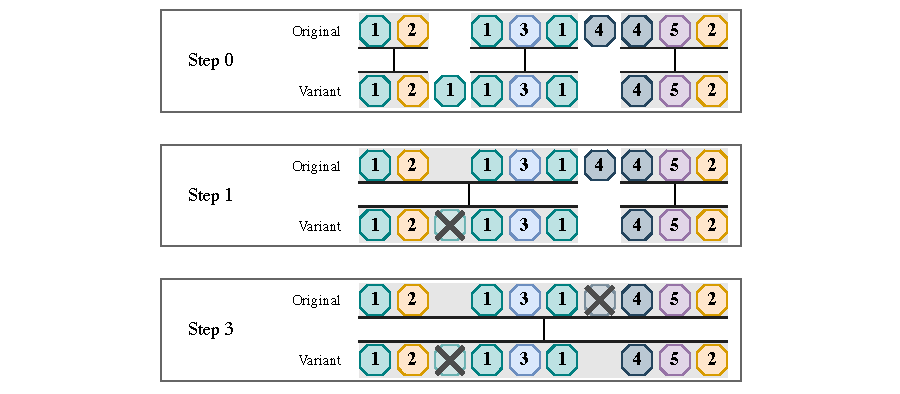
\includegraphics[width=\linewidth]{figures/algorithm/steps.pdf}
\caption[Subsequence Match Merging Example]{Steps of the subsequence match merging for the running example in \autoref{tab:re-tokens} (minimum match length = 4, minimum neighbor length =, 2 and maximum gap-size = 1).}
\label{fig:fullMatchMerging}
\end{figure}

\subsection{Complexity}
The runtime complexity of the \textit{Subsequence Match Merging} algorithm depends on the number of matches $m$ and the efficiency of merging operations.
The runtime complexity depends on the three main operations: Neighbor computation, merging, and pruning.
The neighbor computation scans all matches sequentially to identify adjacent pairs with a $O(m)$ complexity.
Merging a pair of neighbors is an $O(1)$ operation, while pruning matches after all iterations also requires $O(m)$ time.
We check each neighboring pair for the merging criteria and repeat this until no more merges occur.

In the worst case, each algorithm iteration performs an $O(m)$ neighbor computation and processes up to $O(m)$ merges, with a maximum of $m$ iterations if only one merge occurs per iteration. This results in a worst-case complexity of $O(m^2)$. Conversely, in the best case, where merges significantly reduce the number of matches (e.g., halving the matches in each iteration), the algorithm performs $O(\log m)$ iterations, with each iteration requiring $O(m)$ operations for neighbor computation and merging. Consequently, the best-case complexity is $O(m \log m)$.

The length of the token sequences limits the number of matches. For the sake of the complexity, $m$ can thus also be seen as the length of the longer sequence. As the worst-case runtime complexity for greedy string tiling per program pair is \( O(m^3) \) (see \autoref{sec:found-jplag}), subsequence match merging does not increase the runtime complexity of the plagiarism detection process.

\subsection{Hyperparameters}
To fine-tune the algorithm, we provide two primary hyperparameters: the minimum neighbor length and the maximum gap size (see \autoref{subsec:smm-algorithm}). These can be adjusted to, for example, fit the algorithm to a specific dataset.
Both thresholds are critical for tuning the heuristic's aggressiveness in deciding which neighboring matches to merge. Setting a low neighbor length and a high gap size threshold tends to merge unrelated matches, increasing false positives. Conversely, a high neighbor length and a low gap size limit the effectiveness of our approach by failing to detect most instances of plagiarism. 

We conducted a grid search for a suitable default parameterization to address the trade-off between precision and recall.
We explored neighbor length values from 1 to the minimum match length. The minimum match length was chosen as the upper threshold, as matches above this threshold have already been detected. Furthermore, we explore gap size values from 1 to 20. We chose 20 as the upper threshold, representing a significant code fragment. During our grid search, this was confirmed, as the best results occur far below the threshold of 20. After evaluating each combination across various real-world datasets consisting of different assignment types, sizes, and different programming languages, as well as with varying obfuscation attacks, we observed that a minimum neighbor length of 2 and a maximum gap size of 6 yields the strongest resilience against obfuscation attacks.
To recap, this means that neighboring matches are merged only if each match spans at least two tokens and six or fewer tokens separate them.
Thus, we propose these values as default parametrization. However, we also recommend adjusting these hyperparameters for the dataset at hand when using our approach.

Finally, for the number of minimal merges, we recommend a low value of between three and five. By choosing a conservatively low value here, we ensure that this safeguard does not affect the performance of the algorithm for obfuscated programs.

\subsection{Observed Impact}\label{sec:smm-impact}
This section presents initial observations on the effectiveness of subsequence match merging based on real-world data. It is important to note that this is not intended as a comprehensive evaluation but aims to provide an empirical perspective on how the defense mechanism performs in practical scenarios.

When applying subsequence match merging to an exemplary dataset from programming assignments and analyzing its impact, we observe a distinct difference between unrelated program pairs and those where one program was plagiarized and obfuscated to create the other. For instance, in cases of obfuscation through statement insertion using PlagGen~\cite{Broedel2023}, unrelated program pairs experience an average of 3.64 individual merges. In contrast, plagiarism pairs undergo an average of 73.90 merges. This indicates that the merging criteria of the algorithm rarely fulfilled for unrelated solutions but frequently fulfilled for plagiarism pairs, demonstrating the effectiveness of our heuristic. For this exact purpose, we designed the safeguard via a minimal number of merges. 

%\todo{Empiric results PP-19:}
%\todo{27 Plags: MaxGap{count=1552, sum=4945, min=1, average=3,186211, max=12}}
%\todo{351 Unrelated: MaxGap{count=1276, sum=3272, min=1, average=2,564263, max=12}}
%\todo{Means 73.90 individual merges per plag pair but only 3.64 for unrelated pair}

When varying the hyperparameters of the SMM algorithm for the aforementioned dataset, we can observe how the parameterization affects the effectiveness of the algorithm.
\autoref{fig:mm-nl} illustrates this for a varying minimal neighbor length. As previously discussed, this controls how long neighboring matches must be to qualify them for merging. The original and plagiarized programs achieve almost identical similarity values without match merging. The lower the minimal neighbor length, the clearer the separation becomes. We can see how this parameter controls the aggressiveness of the merging. Lower values lead to fewer individual merges and vice versa.

Next, \autoref{fig:mm-nl} illustrates the impact of the hyperparameters for a varying maximal gap size. The gap size controls how many tokens can separate two neighboring matches to still qualify them for merging. Again, without merging, the similarity values collapse. For the gap size, the effectiveness increases when increasing the parameter. However, the effects are less strongly pronounced compared to the neighbor length. Furthermore, the impact of an increasing gap size stagnates at a particular value. In the case of \autoref{fig:mm-nl}, this happens at a gap size of 5 tokens.

In Summary, we can observe that subsequence match merging increases the similarity of plagiarism pairs while maintaining a minor impact on the original and unrelated pairs. With this, subsequence match merging improves the resilience against obfuscation attacks.


\begin{figure}[p]
\centering
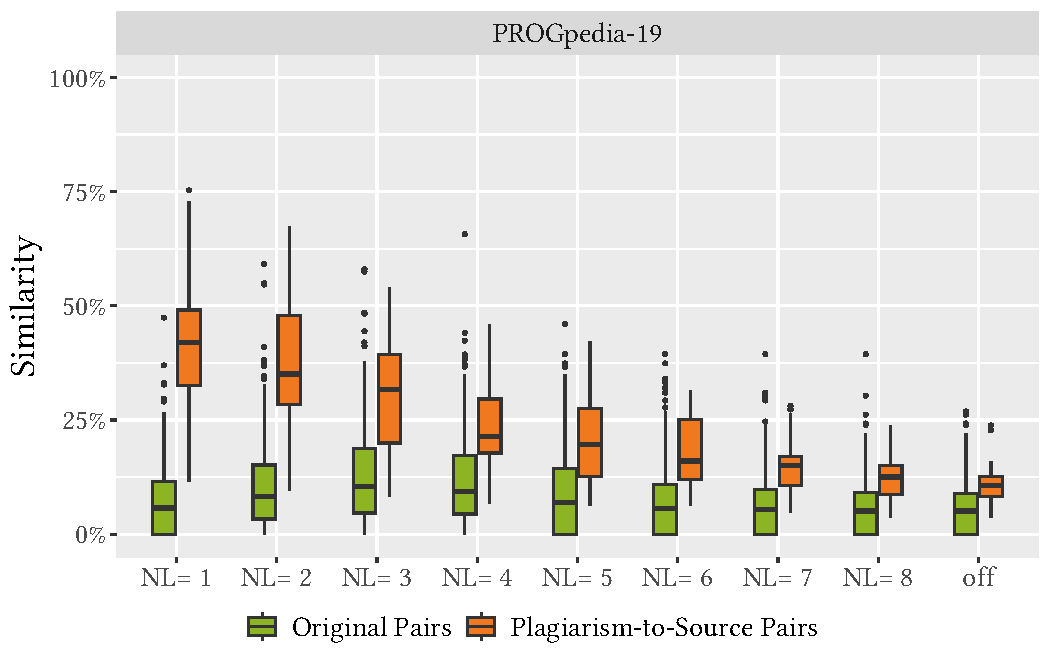
\includegraphics[width=0.95\linewidth]{figures/algorithm/eval-mm-NL_avg.similarity.pdf}
\caption[Impact of the Neighbor Length]{Impact of the hyperparameter neighbor length (NL) for a programming assignment dataset~\cite{paiva2023} and plagiarized programs via insertion-based obfuscation via PlagGen~\cite{Broedel2023}. Plagiarism pairs should be high, while original pairs should be low.}
\label{fig:mm-nl}
\end{figure}

\begin{figure}[p]
\centering
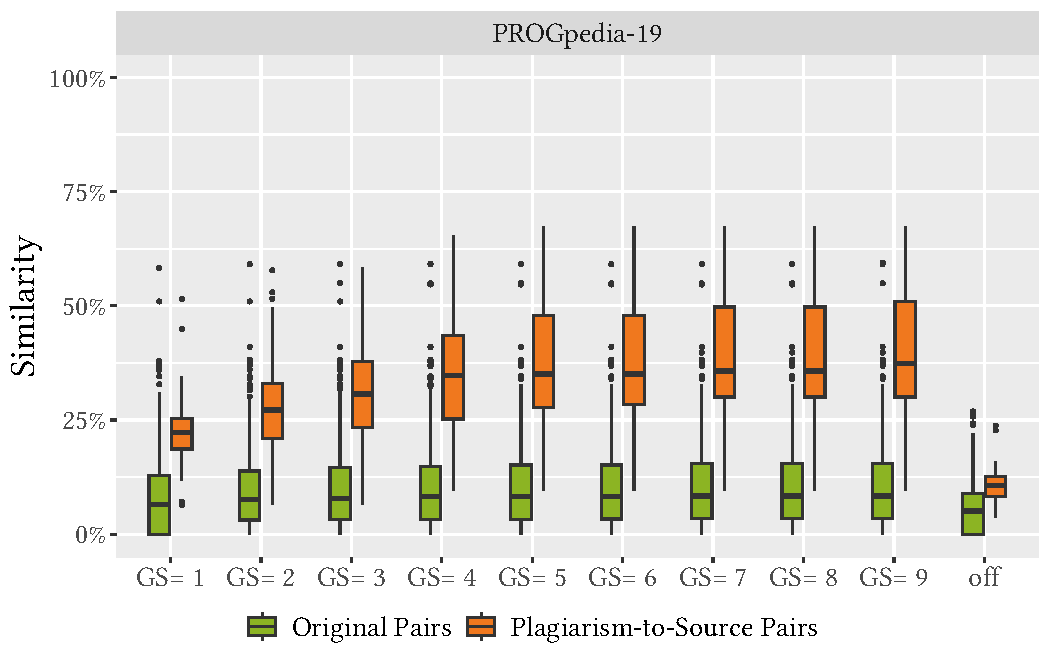
\includegraphics[width=0.95\linewidth]{figures/algorithm/eval-mm-GS_avg.similarity.pdf}
\caption[Impact of the Gap Size]{Impact of the hyperparameter gap size (GS) for a programming assignment dataset~\cite{paiva2023} and plagiarized programs via insertion-based obfuscation via PlagGen~\cite{Broedel2023}. Plagiarism pairs should be high, while original pairs should be low.}
\label{fig:mm-gs}
\end{figure}


\subsection{Limitations}\label{sec:smm-limits}

While subsequence match merging is an effective defense mechanism against various obfuscation attacks, there are some limitations to consider. In the following, we discuss the heuristic nature of the defense mechanism and the choice of suitable hyperparameter values.

    \subsubsection{Heuristic-based Defense}
    The strength of subsequence match merging is that it employs a heuristic to determine which matches to merge.
    Thus, it can provide broad obfuscation resilience, as it requires no knowledge of the specifics of obfuscation attacks.
    However, employing heuristics carries an inherent risk of increasing similarity for unrelated programs, as merging unrelated matches can inadvertently connect unrelated code fragments. This can be the case when a pair of unrelated programs has two sections that are coincidentally similar, and which are separated by a few lines of code in one or both of the programs that are not similar.
    To minimize the impact of match merging on pairs of unrelated programs, we use the original matches whenever too few merging operations are conducted. This significantly reduces the effect on unrelated programs, as for obfuscated programs, many merging operations occur (for example, three to four merges for unrelated programs versus 74 for obfuscated ones, as discussed in \autoref{sec:smm-impact}). 
    Although this mechanism minimizes false positives, subsequence match merging may still slightly increase the similarity of unrelated program pairs.

    \subsubsection{Choice of Hyperparameters}
    We intentionally avoided designing a defense mechanism that relies on too many hyperparameters, as it is always challenging for users to determine an optimal configuration in such cases~\cite{Schmid2022}.
    However, subsequence match merging relies on two hyperparameters (minimum neighbor length and maximum gap size) to determine which subsequences to merge. With a lower minimum neighbor length and a larger maximum gap size, the defense mechanism can revert the effects of stronger obfuscation attacks. However, it is also more prone to merging subsequences that do not belong together, meaning their corresponding code fragments are separated by correctly unmatched code (see \autoref{sec:smm-impact}).
    Incorrect parameter tuning could lead to missed plagiarism cases (under-merging) or excessive false positives (over-merging). To address this issue, we conducted a systematic hyperparameter search on different datasets. We observed that for our datasets, the effects of the hyperparameters are not strong enough to make under-merging or over-merging a probable issue. Specifically, we observed that the hyperparameters mainly affected how well the defense mechanism performed, but the overall detection quality did not fall below the base case, with subsequence match merging disabled.
    From this hyperparameter search, we derived recommended default values for the hyperparameters.
    While these values work well for various datasets, one limitation is that these values are not guaranteed to work for all datasets.
    However, as they are hyperparameters, they can be adapted to the specific dataset at hand.
    
\section{Model Subtree Reordering}\label{sec:msr}
In this section, we introduce our third defense mechanism (\contribution{3.3}) called \textit{model subtree reordering} (MSR)~\cite{Saglam2024a}. 
%
% MOTIVATON
Modeling assignments, such as \ac{UML} class, use case, sequence, and activity models, are common in computer science education~\cite{Ciccozzi2018, Saglam2023}. Modeling is integral to traditional software engineering courses due to the practical use of modeling languages like \ac{UML}. Furthermore, metamodeling assignments are becoming increasingly prevalent with the growing adoption of model-driven techniques~\cite{Brambilla2017, Hutchinson2011}. The complexity of modeling assignments and their demand for domain understanding and problem-solving skills make them susceptible to plagiarism~\cite{Martinez2020}. However, research on detecting plagiarism in modeling assignments is limited~\cite{Martinez2020, Saglam2022, Saglam2023}.

% REQUIREMENT: DEGREES OF FREEDOM
Effective plagiarism detection for modeling assignments necessitates mechanisms to handle degrees of freedom in models. Reordering attacks might exploit this flexible nature of models, which can lead to significant variations in the token sequence extracted from these models. While token-based detection approaches can detect large-scale reordering, for example, reordering methods in a class or classes in a \ac{UML} diagram, they are vulnerable to fine-grained reordering attacks~\cite{Saglam2022}. For program code, statements have a strong interdependence, thus limiting the effectiveness of reordering attacks (realistically, such an obfuscation attack will only reduce the similarity by about five percentage points~\cite{Saglam2024b}). For modeling artifacts, however, these fine-grained reordering attacks can effectively obfuscate plagiarism.
%
% EXAMPLE OF THIS
For example, the order of elements within multi-valued containment references can vary significantly in \ac{EMF} metamodels.
Likewise, in \ac{UML} class models, the order of attributes and methods within a class is often flexible and does not affect the model's semantics. Similarly, the sequence of states and transitions is not semantically significant in state charts. Instead, the critical aspect is the specific state from which a transition originates and the state to which it leads.
%
In the following, we discuss the targeted obfuscation attacks, the fundamental concept of model subtree reordering, the detailed algorithm, its complexity, and the limitations of the defense mechanism.

\begin{factsheet}{Overview: Model Subtree Reordering} 
    \begin{description}[style=multiline,leftmargin=5.5cm]
        \item[Core Principle] Normalize the Order of Elements in the Model
        \item[Targeted Obfuscation Attack] Model Element Reordering
        \item[Language Family] Modelling Languages
        \item[Language Dependence] Language-Agnostic
        \item[Performance Impact] Very Low
        \item[Main Scalability Determinant] Size of Input Models
        \item[Integration Complexity] Moderate
    \end{description}
\end{factsheet}

\subsection{Targeted Obfuscation Attacks}
When using token-based approaches for modeling plagiarism detection, obfuscation attacks based on moving and swapping elements on a fine-grained level pose a viable threat~\cite{Saglam2022} because of the degrees of freedom discussed above.
Consider the view on the \texttt{Store} package in \autoref{fig:example-view}. It depicts two classes with their corresponding attributes, references, and containment references.
For this model view, \autoref{tab:example-view} presents three corresponding token sequences. All three sequences correctly represent the same model elements depicted in \autoref{fig:example-view}. However, the order of tokens varies between the sequences.
The original sequence represents the element order as shown in the graphical view. The first variant is created by swapping the tokens corresponding to each class, slightly altering the token sequence. The second variant is created from the first by reordering the tokens of the features, again modifying the token sequence order completely.
%
These variations in token sequences are a form of obfuscation where the token sequence remains semantically equivalent, but its representation is altered. This is possible for \ac{EMF} or \ac{UML} models, as the order of classes in a package and the order of features in a class have no semantic relevance. This also applies to many other modeling languages. Reordering is also common in source code plagiarism, but there, it provides limited effectiveness~\cite{Saglam2024b}.

Model subtree reordering targets the unique challenges posed by ordering-based obfuscation attacks on modeling artifacts.
To reduce the impact of the degrees of freedom common in modeling artifacts, we normalize the order of tokens corresponding to the elements in the model, ensuring a consistent representation of modeling artifacts and thereby countering obfuscation efforts that rely on the fine-grained reordering elements.
However, normalization in this context is far from trivial.
The properties used for normalization must be selected carefully to avoid introducing new attack vectors, and the process must minimize changes to the token sequence to prevent false positives.
Only \textit{robust} criteria can provide stability and invariance to obfuscation attacks.

\begin{samepage}
\begin{figure}[b]
    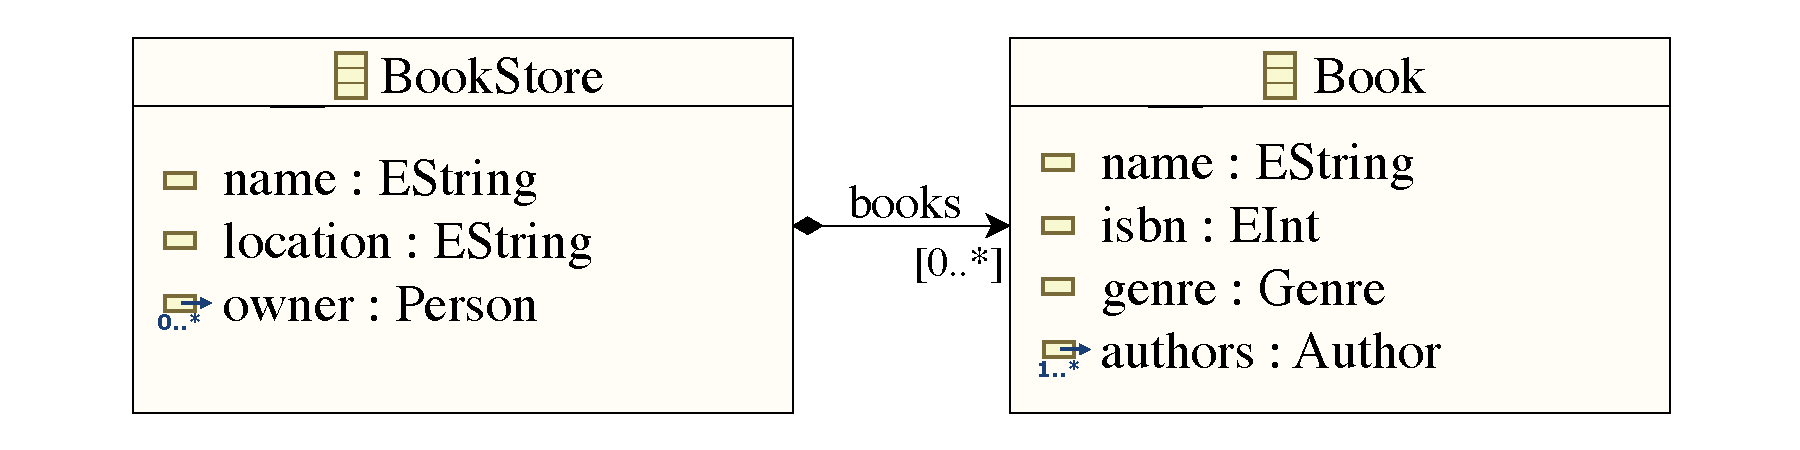
\includegraphics[width=\textwidth]{figures/mde/bookstore-view.pdf}
    \caption[Bookstore Model View]{View on the package \texttt{Store} of the second bookstore management system model as shown in \autoref{fig:running-example}, depicting two classes with their attributes and references.}
    \label{fig:example-view}
%\end{figure*}
\end{figure}

\begin{table}[b]
    \centering
    %\small
    \begin{tabular}{clll}
		\toprule
		\# & \textbf{Original}     & \textbf{Variant 1}    & \textbf{Variant 2}    \\
		\midrule
		1  & \texttt{Class}        & \texttt{Class}        & \texttt{Class}        \\
		2  & \texttt{ Containment} & \texttt{ Attribute}   & \texttt{ Attribute}   \\
		3  & \texttt{ Attribute}   & \texttt{ Attribute}   & \texttt{ Reference}   \\
		4  & \texttt{ Attribute}   & \texttt{ Attribute}   & \texttt{ Attribute}   \\
		5  & \texttt{ Reference}   & \texttt{ Reference}   & \texttt{ Attribute}   \\
		6  & \texttt{Class End}    & \texttt{Class End}    & \texttt{Class End}   \\
		7  & \texttt{Class}        & \texttt{Class}        & \texttt{Class}    \\
		8  & \texttt{ Attribute}   & \texttt{ Containment} & \texttt{ Attribute}   \\
		9  & \texttt{ Attribute}   & \texttt{ Attribute}   & \texttt{ Reference} \\
		10 & \texttt{ Attribute}   & \texttt{ Attribute}   & \texttt{ Containment}   \\
		11 & \texttt{ Reference}   & \texttt{ Reference}   & \texttt{ Attribute}   \\
		12 & \texttt{Class End}    & \texttt{Class End}    & \texttt{Class End}    \\
		\bottomrule
    \end{tabular}
    \caption[Example Obfuscation: Reordering]{Three token sequences, all representing the model view depicted in \autoref{fig:example-view}. The original reflects the element order of the view, while the first variant is created by swapping the tokens of each class, and the second variant is created from the first by reordering the tokens of the features. Note that all references are multi-valued, which is omitted for readability.}
    \label{tab:example-view}
\end{table}
\end{samepage}

Simple approaches like sorting by type or lexical order are insufficient, as they can be easily manipulated by specific obfuscation attacks (e.g., element insertion or property changes). The normalization is either ineffective or can be affected via specific obfuscation attacks.
For example, consider a hypothetical normalization based on element names: Whenever named model elements can be in an arbitrary order, they are sorted lexically via their names. While this provides resilience against reordering, it also includes vulnerability against renaming, as minor name changes now affect the element order. Besides names, other vulnerable properties include identifiers, data types, values, and other literals.
Normalization properties must be stable, invariant, and meaningful to detect plagiarism accurately and effectively.
Thus, robust properties are only based on the information already used by the plagiarism detectors and are limited to the extracted tokens corresponding to the patterns and structural patterns in these tokens.


\subsection{Concept}
As discussed in \autoref{sec:mde-approach}, tokenization references refer to the meaningful connections between elements in a model that capture the underlying semantics of the modeled system. Unlike syntactic references, which focus on the structural aspects of the model, tokenization references emphasize the relationships and dependencies that convey the intended behavior and functionality. 
Again, consider a state chart model. While structurally, all states might be contained under a common root element, these containment references are syntactic references. The underlying semantics are modeled by transition references between states, which are thus considered tokenization references.
These references are crucial for accurately detecting plagiarism in modeling assignments, as they ensure that the detection mechanisms account for the intent and semantics behind the models rather than just superficial similarities. By leveraging tokenization references, we can improve the robustness of modeling plagiarism detection. However, this also means these tokenization references must be identified for each modeling domain, as this distinction is purely conceptual and not reflected in the actual modeling artifacts.

Model subtree reordering is designed against reordering attacks by specifically leveraging these tokenization references to normalize the order of the token sequence. 
The approach applies to any modeling artifact with a tree-like structure where tokenization references can be identified. However, the effectiveness of this method depends on the extent of variability allowed within these types of artifacts.
%
To ensure a deterministic order in the token sequences representing modeling artifacts, we sort the elements in each multi-valued tokenization reference first based on their token type and then based on the distribution of the tokens in their subtree of direct and indirect children.
While the former is a coarse-grained ordering criterion to group model elements that map to the same token type, the latter is a more fine-grained one to capture and preserve the structural nuances within subtrees of the referenced elements.

At a high level, our approach leverages the concept of token type vectors to represent the structure of the model subtree. These vectors capture the frequency of various token types within the subtree, allowing us to compare and sort elements based on their structural characteristics. Thus, such a vector represents the distribution of different kinds of model elements in a specific part of the model. For example, we can consider the three subtrees illustrated in \autoref{fig:tree-examples}. Note that these are token trees, meaning the structure defined by the tokenization references of a model where each model element is replaced by its corresponding token. While all three trees are similar, subtree A has a different distribution of tokens than subtrees B and C, as each type (represented by color) occurs only once. While the subtrees B and C are structurally different, they share the same distribution of tokens. Note that the tree B can be transformed into the tree B with a single reordering operation.

If we now interpret these vectors as points in a multi-dimensional space, we can use the distance of these points to estimate how structurally similar two parts of a model are. By finding a path (meaning a sequence that includes all points) in this space that minimizes the distance between points, we can derive an order that is both deterministic and not easy to affect intentionally. This approach ensures that structurally similar elements are consistently ordered, thereby mitigating the effects of obfuscation through reordering while maintaining the stability of the normalization process.


\begin{figure}
    \centering
    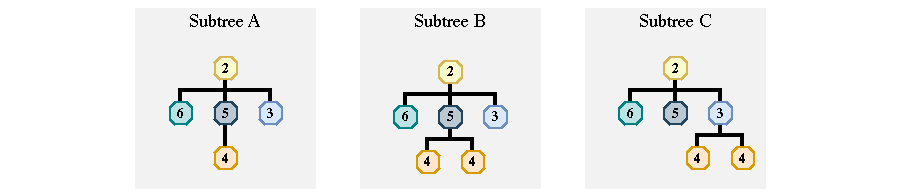
\includegraphics[width=\linewidth]{figures/mde/subtree-examples.pdf}
    \caption[Model Subtree Examples]{Three exemplary model subtrees based on tokenization references in token representation, where subtree A contains a slightly different token distribution than subtrees B and C, which share the same distribution.}
    \label{fig:tree-examples}
\end{figure}


\subsection{Algorithm}
Our normalization algorithm consists of several steps. The entire algorithm is listed in \autoref{alg:NormalizationAlgorithm}.
We begin by generating tokens for each element's subtree and then create a token type vector that indicates how often each type of token occurs within that subtree. For instance, in the case of the class \texttt{Book} depicted in \autoref{fig:tokenization}, this vector is represented as $[2, 1, 1, 0, \dots, 0]$, where the vector components correspond to two attributes, one identifier attribute, and one reference.
To enable meaningful comparisons between these vectors, we first normalize them. The normalization is done by computing the Euclidean norm of each vector:
\begin{align*}
    \|\mathbf{v}\|_2 = \sqrt{\sum_{i=1}^{n}v_i^2}
\end{align*}
This normalization process scales the vectors to have a length of 1, ensuring that the comparison between them is not influenced by the absolute magnitude of the original vectors but by the distribution of token types within each subtree.
Once normalized, these vectors can be interpreted as points in a multi-dimensional coordinate space, where each dimension corresponds to a specific token type. The position of each point in this space is determined by the distribution of token types in the corresponding element's subtree. For example, a vector with more attributes will be closer to the axis representing attributes.

To compare these points (representing different elements), we calculate the Euclidean distance between any two points $\mathbf{p}$ and $\mathbf{q}$ using the following metric:
\begin{align*}
    d_{\mathrm{E}}(\mathbf{p}, \mathbf{q}) = \sqrt{\sum_{i=1}^n (q_i-p_i)^2}.
\end{align*}
Using these distances, we construct a nearest neighbor path that sequentially connects each point to its closest neighbor, starting from the point associated with the element with the most tokens in its subtree. This ordering method prioritizes elements with greater structural complexity, which helps preserve the overall structure during the normalization process.
%
In cases where two or more points are equidistant from the last point in the path, we resolve the tie by referring to the original order of the elements. This ensures that the normalization process is stable, meaning that the same input will always produce the same normalized output, avoiding the introduction of inconsistencies due to random ordering.
%
%
Finally, to normalize the order of elements within a tokenization reference, we apply a two-step sorting process:
    \begin{enumerate}
        \item Primary Sorting by Token Type: We first sort the elements based on their token type vectors, providing a coarse-grained ordering that groups similar elements.
        \item Secondary Sorting by Nearest Neighbor Path: If two elements have identical token type vectors, we further sort them according to their position in the calculated nearest neighbor path. This fine-grained sorting helps maintain the relative order of structurally similar elements.
    \end{enumerate}
This approach ensures that the elements within a model are consistently ordered, thereby countering potential obfuscation strategies that rely on reordering elements.


\autoref{fig:tokentreenorm} illustrates the process of reordering tokens for three elements within the same (multi-valued) tokenization reference. The normed subtree vectors are used to calculate the elements' distances, sorting the elements according to the computed nearest neighbor path.
\begin{enumerate}
    \item {Token Tree}: We start with the token trees for three classes, each containing various tokens that represent different model elements such as identifiers, attributes, and references.
    \item {Subtree Vectors}: As a first step, the algorithm generates subtree vectors for each class, denoted as \( \mathbf{v}_a \), \( \mathbf{v}_b \), and \( \mathbf{v}_c \). These vectors count the occurrences of each token type within the subtrees. For example, the subtree vector for \texttt{Class} $a$ is \( \mathbf{v}_a = [1, 1, 0, \dots, 0] \), indicating one identifier and one attribute.

    \item {Normalized Vector}: Next, each subtree vector is normalized by its Euclidean norm \( \|\mathbf{v}\|_2 \). The normalized vectors represent the scaled distribution of tokens, ensuring comparability regardless of their original magnitude.

    \item {Euclidean Distance}: The normalized vectors are then used to calculate the Euclidean distance between each pair of elements. The distance matrix \( D \) encapsulates these distances, with each entry \( d_{ij} \) representing the distance between the vectors of \texttt{Class} $i$ and \texttt{Class} $j$. For example, the distance between \( \mathbf{v}_a \) and \( \mathbf{v}_b \) is \( d_{ab} = 0.765 \).

    \item {Nearest Neighbor Path}: Using the distance matrix \( D \), the algorithm determines the nearest neighbor path. The path starts from the element with the largest subtree (in this case, \texttt{Class} $b$) and proceeds by selecting the nearest neighbor at each step.

    \item {Normalized Token Sequence}: Finally, the model elements are reordered according to the nearest neighbor path, resulting in a normalized token sequence.
\end{enumerate}


\begin{figure}
    \centering
    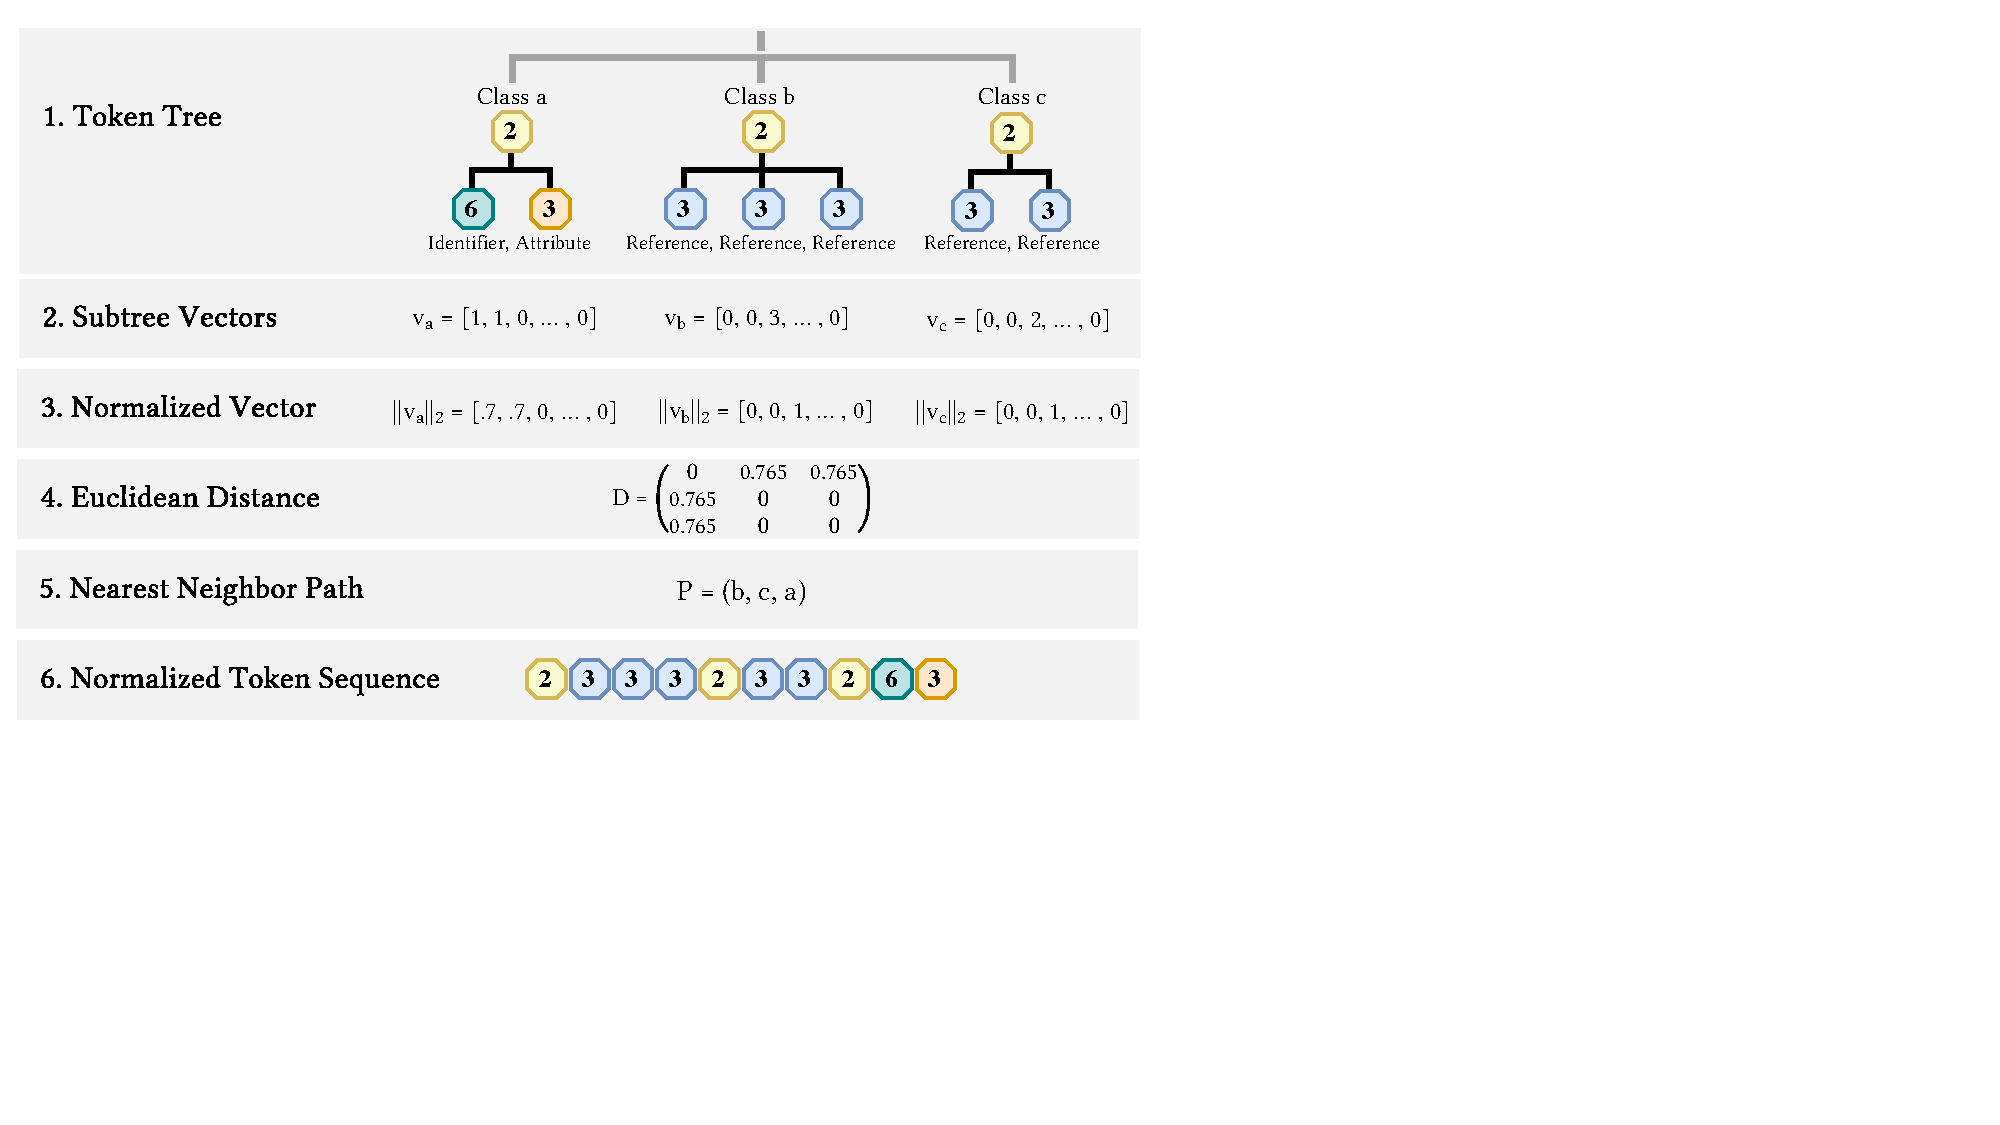
\includegraphics[width=0.9\linewidth]{figures/mde/normalization-new.pdf}
    \caption[Model Subtree Reordering Example]{Example illustrating how model subtree reordering normalizes the token sequence via element reordering for a multi-valued reference containing three classes.}
    \label{fig:tokentreenorm}
\end{figure}

\begin{algorithm}
    %\captionsetup{belowskip=-\baselineskip}
	\caption{Model Subtree Reordering}
	\label{alg:NormalizationAlgorithm}
	\begin{algorithmic}
		\Require{List of model elements $E$ with length $n$}
		\Function{Normalize Token Sequence}{$E$}
		\State{$V \gets$ empty list of vectors}
        \For{$e_i \in E$}
		      \State{$v_i \gets$ calculate token type vectors for subtree of $e_i$}
            \State{$v_i \gets$ euclidean norm $\|\mathbf{v_i}\|_2 $}
		\EndFor
  
        \State{$D \gets$ empty distance matrix with size $n \times n$ }
		\For{$v_i, v_j \in V$}
		      \State{$d_{i,j} \gets$ euclidean distance $d_{\mathrm{E}}({v_i}, {v_j})$}
		\EndFor
  
		\State{$v_{max} \gets$ vector in $V$ of element with largest subtree}
            \State{$P \gets$ nearest neighbor path for $D$ starting from $v_{max}$}
            \State{$S \gets$ sort $E$ by token type, if equal by position in $P$}
            \State{\Return{$S$}}
		\EndFunction
	\end{algorithmic}
\end{algorithm}

% OLD VERSIONS
%\input{tables/normalization}

\noindent

In our approach, we opted to use the nearest neighbor path rather than the shortest path, as the nearest neighbor path is more robust against modifications in the subtrees. The shortest path, which typically minimizes the total distance between points in a coordinate space, can be sensitive to even minor changes in the structure of the elements, potentially leading to significant shifts in the ordering. Such sensitivity would make the normalization less robust.

On the other hand, the nearest neighbor path focuses on maintaining local consistency by linking each point to its closest neighbor, regardless of the overall path length. This method ensures that small changes in the subtree structure do not disproportionately affect the overall sequence, making the path, and hence the normalization, more resilient to obfuscation techniques that involve subtree modifications.

We further enhance the robustness of the normalization by carefully choosing the starting point for constructing the nearest neighbor path. Specifically, we start from the element with the most tokens in its subtree. This choice is based on findings from our pre-study, which indicated that beginning with the most complex (or structurally significant) element leads to a normalization more resistant to reordering attacks. The rationale is that the element with the most tokens likely has a more pronounced impact on the overall model structure, making it a stable anchor for the normalization process.

Using the nearest neighbor path and selecting a strategic starting point, our approach effectively addresses the normalization challenge in modeling plagiarism detection. It ensures that similar structures are consistently ordered in a way that is less susceptible to manipulation. This combination of strategies—prioritizing local consistency and starting with the most significant element—provides a more stable and reliable method for detecting plagiarism in models.


\subsection{Complexity}
The runtime complexity of the model subtree reordering algorithm in \autoref{alg:NormalizationAlgorithm} depends on the tree defined by the tokenization references and is thus influenced by the size of the subtrees and the number of model elements. Note that a tree with $m$ nodes can have a maximum of $m$ subtrees when every node except the root is a leaf. Furthermore, the maximum number of tokens in a subtree is limited by $m$.

The runtime complexity of model subtree reordering depends on the three main operations: Calculating the token type vectors, computing the distance matrices, constructing the distance matrices, and sorting the subtrees via a nearest neighbor search.
%
For an entire model of $m$ elements, the token type vectors for each subtree can be calculated via a single depth-first search with the runtime complexity of $O(m)$.
Constructing the distance matrix involves computing pairwise distances for up to $m-1$ elements (when all model elements are leaves of a single root), which contributes $O(m^2)$ complexity.
Sorting of all elements according to their distances via a nearest neighbor search has a complexity of $O(m \log m)$.

The overall runtime complexity is thus $O(m^2)$.
As the worst-case runtime complexity for greedy string tiling per program pair is \( O(m^3) \) (see \autoref{sec:found-jplag}), model subtree reordering does not increase the runtime complexity of the plagiarism detection process.

\subsection{Limitations}\label{sec:msr-limits}
While model subtree reordering is a robust defense mechanism against reordering-based obfuscation attacks for modeling artifacts, it does have certain limitations. In the following, we discuss its dependence on tokenization references, the focus of the defense mechanism, and the effect on unrelated models.

%\begin{enumerate}
    \subsubsection{Dependence on Identifying Tokenization References} As our general approach to modeling plagiarism detection, model subtree reordering 
    depends on the modeling domain and language (see \autoref{sec:mde-limit-domain}). Model subtree reordering operates on stable tokenization references to establish a normalized order. For tree-based models like \ac{EMF} models or \ac{UML} class models, these tokenization references are the containment relations. However, identifying these references is not trivial for some modeling languages and may require domain-specific adjustments for different modeling languages (see \autoref{subsec:tokenization}). This dependency on domain knowledge limits the mechanism as it increases the complexity of applying it to new modeling languages. Nevertheless, this domain-specific adjustment is required to apply our detection approach in the first place and is, thus, no additional effort for model subtree reordering.
    
    \subsubsection{Focused Resilience} model subtree reordering is designed to mitigate reordering attacks by normalizing the token sequence based on model element distributions in subtrees. However, it does not provide resilience against other forms of obfuscation, such as inserting irrelevant model elements. %Such attacks can introduce variability that model subtree
    Although model subtree reordering leverages token subtree distributions, which are much more robust than simpler, vulnerable criteria (e.g., names), substantial modifications to specific parts of a model can still impact the normalization. Such modifications would require significant changes, such as inserting entirely new subtrees, rather than minor adjustments, like adding individual elements. The reason for this is the sorting via nearest neighbor paths, which is not affected by minor changes to the token vectors.
    Even with these large-scale modifications, the effect on obfuscation may remain limited, as inserting new subtrees only partially disrupts the ordering.
    To address cases where the normalization provided by model subtree reordering is affected, model subtree reordering can be combined with subsequence match merging, which combines focused and broad resilience.

    \subsubsection{Effect on Unrelated Models}
    Another limitation of model similarity reordering is that any normalization process can inadvertently increase the similarity of unrelated models. As a normalization technique seeks to resolve ambiguities and standardize representations, it may lead to a situation where models that initially exhibit different structures appear more similar due to the reordering.
    As for all normalization techniques, the question with model subtree reordering is how pronounced this effect is.
    As token subtree reordering is a very abstract technique that only considers the tokens themselves to limit itself to a robust normalization criterion, its normalization of the token order is very broad. In contrast, token sequence normalization only reorders tokens of statements that are not interdependent. Model subtree reordering generally reorders all model elements for each tokenization reference. Thus, it may also affect unrelated models.
    This issue may be less significant for larger models, as they generally produce larger token subtrees with a more complex token distribution. This complexity results in more unique vectors for reordering based on the nearest neighbor paths. In contrast, smaller models do not benefit from this complexity, making the effects of normalization on unrelated models potentially more pronounced.
  
\section{Exploring Additional Defense Mechanisms}\label{sec:other-defense}
This section briefly mentions additional defense mechanisms we explored alongside those mentioned in the previous sections. However, the now-mentioned defense mechanisms have limited language independence or do not fulfill the essential requirements defined in \autoref{sec:tsn-requirements}.
Despite these approaches not being the core contributions of this dissertation, we still want to provide an overview of them. %Furthermore, we compare them to our primary defense mechanisms.

\textbf{Structural Normalization via Code Property Graphs}~\cite{Maisch2024}: We explored an approach to extracting the token sequence of programs from code property graphs instead of parse trees. Before tokenization, we normalize the code property graphs via graph transformations to counter semantic-preserving refactoring-based obfuscation attacks.
This includes refactoring operations like extracting expressions as variables or constants, introducing constant container classes, swapping if-else statements and inverting the corresponding conditions, inserting methods and constructors, and introducing access methods for existing fields.
Similarly to tokens, the sequence normalization approach can also be used to normalize the order of statements and to remove dead code. This approach can be seen as an extension of token sequence normalization. However, it is entirely language-dependent, as tokenization is based on code property graphs, and the corresponding transformations have to be defined for each programming language.

\textbf{Normalization via LLVM IR}~\cite{Heneka2023}: LLVM uses an intermediate representation language resembling assembly code. LLVM supports transforming code in multiple languages into LLVM IR code. During this transformation, code can be heavily optimized. This includes, for example, dead code removal. We investigated plagiarism detection via this intermediate representation. While it does provide resilience for specific obfuscation attacks, it has some drawbacks. First, the LLVM IR code is platform-dependent; thus, the results vary depending on the system architecture. Second, only some languages are supported by LLVM. Finally, the visualization limits the approach, as it shows matches on the IR code. This approach resembles the approach proposed by \citet{DevoreMcDonald2020} of using assembly code for plagiarism detection.

\textbf{Compiler-based Preprocessing}~\cite{krieg2022}: Some compilers provide aggressive preprocessing techniques to optimize program code. This often includes dead code removal and could be used to reduce the impact of some obfuscation attacks. However, this is a pure pre-preprocessing technique (thus falling short for nearly all requirements defined in \autoref{sec:tsn-requirements}) that is strongly language-dependent and provides only limited resilience.

These defense mechanisms provide obfuscation resilience but have disadvantages regarding language dependence or the abovementioned requirements. In the following, we also mention two approaches that are not sufficiently effective in providing obfuscation resilience.

\textbf{Pre-matching Token Filtering}~\cite{krieg2022}: We explored an approach based on sliding windows that filter the token sequences before the actual subsequence matching to reverse the splitting of matches. This heuristic approach was computationally expensive and only somewhat effective when combined with other defense mechanisms. However, this approach inspired our approach of merging subsequence matches. Both approaches share that they are language-independent and attack-independent.
    
\textbf{Token Transformation Patterns}~\cite{krieg2022}: Here, we explored defining a set of token patterns based on the different token types that, if detected in a token subsequence, would lead to the removal of tokens. An example would be the removal of all tokens between a return statement and the end of a block or method. However, these patterns are strongly token-dependent and only provide resilience for specific obfuscation attacks. This only provides limited resilience even among a single attack type, such as insertion-based obfuscation.

\endinput



\begin{table}[b]
	\centering
	\footnotesize
	\begin{tabular}{p{4cm}ccccc}
		\hline
		Defense Mechanisms & Target & Lang.-Ind. & Eff. & Scope & Obfucations \\
		\hline
	    SMM & Both & ++ & ++ & Wide & Any \\ 
		TSN & Code & + & +++ & Narrow & Insertion, Reordering \\
		MSR & Models & + & ++ & Narrow & Reordering \\ 
		Intermediate Representation & Code & o & + & Wide-ish & Many \\ 
         \hline
		Code Property Graphs & Code & o & ++ & Narrow & Refactoring \\ 
		Compiler-based Pre-Processing & Code & $--$ & o & Narrow & Insertion \& Others \\ 
		Token Transformation Patterns & Code & $--$ & - & Narrow & Insertion \& Others \\
		Token Sequence Filtering & Both & ++ & o & Wide & Any \\
		\hline
	\end{tabular}
	\caption[Overview on All Defense Mechanisms]{TODO}
    \todo{TODO}
\end{table}


\part{Evaluation}
\chapter{Evaluation Methodology}\label{cha:methodology}
This chapter outlines the methodology used to evaluate the effectiveness of the proposed contributions regarding obfuscation resilience and detection quality.
We evaluate our primary contributions \contribution{2} (see \autoref{sec:mde-approach}) and \contribution{3} (see \autoref{cha:defense}) \textit{separately}, as they follow different evaluation goals and we apply different baselines, as well as datasets.
%
We evaluate our defense mechanisms (\contribution{3}) regarding obfuscation resilience with the plagiarism detector JPlag as the baseline, as it is not only considered state-of-the-art~\cite{Aniceto2021} but also the most referenced and compared to approach~\cite{Novak2019}.
Furthermore, we evaluate our approach to modeling plagiarism detection (\contribution{2}) regarding its overall effectiveness with the approach of \citet{Martinez2020} as a baseline, as it is, to our knowledge, the only other detection approach for modeling artifacts.
Finally, our threat model (\contribution{1}, see \autoref{cha:threatmodel}) is the foundation for this evaluation, as we systematically employ different obfuscation attacks to evaluate our contributions. 

We use real-world datasets from different university courses, including both programming and modeling assignments. These courses range from mandatory undergraduate courses to master 's-level elective courses. Furthermore, they contain different-sized programs, from smaller ones with around 100 lines of code to large final projects with around 1500 lines of code.
With both evaluation parts, we employ a total of \textit{nine} different obfuscation techniques for the plagiarism instances:
Insertion, deletion, reordering, refactoring, renaming, simulated random alteration, AI-based obfuscation, AI-based implementation, and human obfuscation.
We thus systematically address all categories introduced in our threat model (see \autoref{fig:clone-types}).
%
Over the entirety of this evaluation, we analyze over \textit{4.1 million data points}, each representing a similarity value of a pairwise comparison of two programs. The datasets sum up to over 14,000 files with over a million source lines of code (\textit{excluding} blank lines and comments). Around 978,000 lines stem from the programming datasets, while around 33,000 lines stem from the modeling datasets (for models, we count the lines in the persisted \ac{XMI} files).

In this chapter, we outline our evaluation methodology. We begin by presenting the evaluation goals using a \textit{Goal-Question-Metric} plan. Next, we discuss similarity metrics and statistical measures. We then justify our choice of baselines -- JPlag for code plagiarism and a \ac{LSH} based approach~\cite{Martinez2020} for modeling plagiarism. Finally, we describe our datasets.

\ownpublications{
    \fancycite{Saglam2024b},
    \fancycite{Saglam2024a},\\
    \fancycite{Saglam2024d}, and
    \fancycite{Saglam2024c}.
}

\section{Evaluation Goals}
The evaluation follows the \textit{Goal-Question-Metric} (GQM) method~\cite{Basili1984, Basili1992}. We thus present a detailed \gqm{} below. We define two conceptual goals for the evaluation, specify corresponding evaluation questions that allow deciding if the goals were fulfilled, and introduce metrics as measures to answer their corresponding questions.
%\todo{overarching GQM plan or evaluation goals to bring both parts together}
%\todo{mapping on contributions}

The first goal, \gref{1}, maps to our primary contribution \contribution{3} and focuses on providing resilience against automated obfuscation attacks for programming assignments. The evaluation in this context explores the ability of a plagiarism detector to withstand various obfuscation attacks. Additionally, the evaluation addresses the effectiveness of the system in distinguishing AI-generated programs from human-written ones.
Here, we compare the baseline performance of the detector and its performance with our contributions.
The corresponding questions investigate the degree of resilience that can be achieved for each obfuscation type. The metrics are centered around the difference in similarity values between pairs of plagiarized and original programs and between AI-generated and human programs. 
%
As plagiarism detectors compute similarity scores for pairs of programs, we thus measure the difference between the scores for the plagiarism instances compared to other, unrelated program pairs.
%
Furthermore, we conduct comprehensive statistical tests (we discuss all metrics in detail in the following section, see \autoref{def:delta-metrics}).
%
Crucially, the evaluation also considers the effects on unrelated programs and the effects of our contributions on threshold-based obfuscation. For the former, the metric of choice is the similarity values for all pairs of unrelated programs.
For the latter, the metrics measure the obfuscation time and the program size after the obfuscation.

The second goal, \gref{2}, maps to \contribution{2} and also to \contribution{3} and aims to enable token-based plagiarism detection for artifacts of modeling assignments. The questions inquire whether token-based plagiarism detection methods can be applied to modeling artifacts and how well these methods perform compared to the state-of-the-art approach proposed by \citet{Martinez2020}. Furthermore, they focus on the provided resilience to obfuscation attacks in modeling assignments.
The corresponding metrics are thus centered around the difference in similarity values between pairs of plagiarized and original models.
%
The obfuscation types addressed in the questions under G1 and G2 map directly to the threat model associated with \contribution{1}.

\clearpage
\begin{description}\label{main-gqm}
    \label{gqm-plan}
    \item[\large{Goal-Question-Metric Plan:}]
    \normalsize
    \item[G1] Provide resilience against automated obfuscation attacks for programming assignments.
        \begin{description}[style=unboxed]
            \footnotesize
            \item[Q1.1] To what degree do our contributions affect the similarity scores of unrelated programs?
                \begin{description}[style=unboxed]
                    \footnotesize
                    \item[M1.1] Similarity values for pairs of original programs.
                \end{description}
            \item[Q1.2] What degree of resilience do our contributions achieve against insertion-based obfuscation?
                \begin{description}[style=unboxed]
                    \footnotesize
                    \item[M1.2] Similarity value differences between plagiarized and original programs (\autoref{def:delta-metrics}).
                    %\item[M1.2] Difference in similarity values between pairs of plagiarized and original programs.
                    \item[M1.3] Statistical significance for M1.2 (p-values).
                    \item[M1.4] Practical significance for M1.2 (effect size).
                \end{description}
            \item[Q1.3] What degree of resilience do our contributions achieve against alteration-based obfuscation?
                \begin{description}[style=unboxed]
                    \footnotesize
                    \item[\textit{(see Q1.2)}]
                \end{description}
            \item[Q1.4] What degree of resilience do our contributions achieve against refactoring-based obfuscation?
                \begin{description}[style=unboxed]
                    \footnotesize
                    \item[\textit{(see Q1.2)}]
                \end{description}
            \item[Q1.5] What degree of resilience do our contributions achieve against AI-based obfuscation?
                \begin{description}[style=unboxed]
                    \footnotesize
                    \item[\textit{(see Q1.2)}]
                \end{description}
            \item[Q1.6] How well can we distinguish AI-generated from human programs?
                \begin{description}[style=unboxed]
                    \footnotesize
                    \item[M1.5] Similarity value differences between generated and student programs (\autoref{def:delta-metrics}).
                    \item[M1.6] Statistical significance for M1.5 (p-values).
                    \item[M1.7] Practical significance for M1.5 (effect size).
                    %\item[M1.5] Difference in similarity values between pairs of generated and human programs.
                \end{description}
            \item[Q1.7] What impact do our contributions have on threshold-based plagiarism generators?
                \begin{description}[style=unboxed]
                    \footnotesize
                    \item[M1.8] Difference in the runtime of the plagiarism generator.
                    \item[M1.9] Difference in number of inserted lines in the plagiarism instance.
                \end{description}
        \end{description}
    \item[G2] Enable token-based plagiarism detection for modeling assignments.
        \begin{description}[style=unboxed]
            \footnotesize
            \item[Q2.1] Can token-based plagiarism detection be applied to modeling artifacts?
                \begin{description}[style=unboxed]
                    \footnotesize
                    \item[M2.1] Similarity value differences between plagiarized and original models (\autoref{def:delta-metrics}).
                    %\item[M2] Difference in similarity values between pairs of plagiarized and original models.
                    \item[M2.2] Statistical significance for M1.2 (p-values).
                    \item[M2.3] Practical significance for M1.2 (effect size).
                \end{description}
            \item[Q2.2] How well does it perform compared the state-of-the-art by \citet{Martinez2020}?
                \begin{description}[style=unboxed]
                    \footnotesize
                    \item[\textit{(see Q2.1)}]
                \end{description}
            \item[Q2.3] What degree of obfuscation resilience can we achieve?
                \begin{description}[style=unboxed]
                    \footnotesize
                    \item[\textit{(see Q2.1)}]
                \end{description}
                
        \end{description}
\end{description}

\section{Similarity Metrics}\label{sec:metrics}

As plagiarism detection systems compute similarity scores for pairs of programs (see \autoref{sec:threatmodel-algebra}), these scores are the primary underlying indicator to consider when evaluating such detection systems.
When using plagiarism detection systems in practice, this score is used as a primary decision-maker for which suspicious candidates to inspect first.
As no objective features can definitively identify plagiarism, the results produced by these systems should always be combined with human judgment.

Usually, plagiarism detection systems provide a visualized distribution of all similarities in a set of programs and a ranked list of pairs sorted by similarity to identify potential suspicious outliers quickly.
Both, however, are directly derived from the similarity scores.
This means the similarity scores strongly guide the human inspection. The detailed view of matching subsequences visualized via matching code fragments is usually then used only after deciding which candidates to inspect. Furthermore, additional post-processing information is usually considered a secondary indicator.
%\textcolor{red}{However, it's important to consider that similarity metrics significantly impact human decision-making, as the interface presenting these scores can bias instructors toward higher-similarity cases and might result in overlooking more subtle instances of plagiarism.}

Between different plagiarism detection systems, the exact calculation of the similarity score for pairs of programs may vary. The difference is usually subtle, and its effect on the overall results is negligible. In our evaluation, we use the similarity score as calculated by JPlag~\cite{prechelt2000} as it is used as a baseline. This \textit{symmetric similarity} score is detailed in \autoref{theo:avgsim}.


\begin{figure}[b]
    \centering
    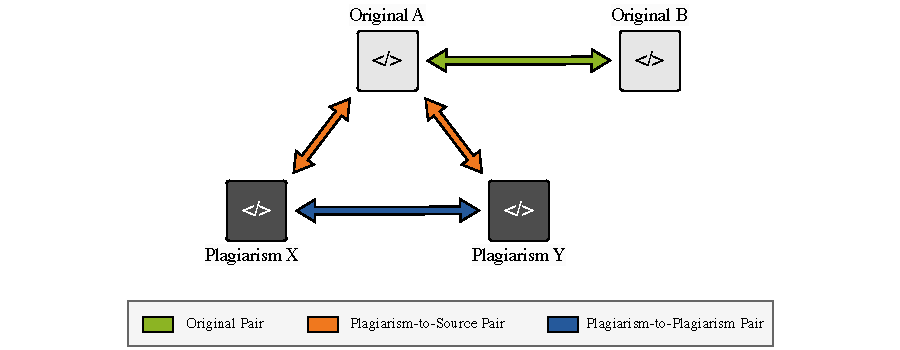
\includegraphics[width=0.95\linewidth]{figures/methodology/Metrics-Pairs.pdf}
    \caption[Different types of Program Pairs]{Visualization of different pairs of programs in the context of plagiarism detection.}
    \label{fig:pair-types}
\end{figure}

When evaluating plagiarism detection systems regarding their detection quality, we need to consider different types of program pairs:
%Plagiarism pairs, consisting of a plagiarism instance and its source program, and unrelated pairs, consisting of two unrelated, original programs.
\begin{enumerate}
\item \textit{Original Pair}: Two unrelated, original programs where no plagiarism was involved.
\item \textit{Plagiarism-To-Source Pair}: A plagiarism instance and its source program.
\item \textit{Plagiarism-To-Plagiarism Pair}: Two plagiarism instances of the same source program.
\end{enumerate}
\autoref{fig:pair-types} illustrates these types of pairs. Note that plagiarism-to-plagiarism pairs only exist when multiple plagiarized instances are created from a single source program. The color scheme in this figure will be used in the remainder of this evaluation for the corresponding pair types.

To clearly distinguish the plagiarism instances from the unrelated programs during human inspection, the similarity scores of plagiarism pairs must be high~\cite{Saglam2024b}. Vice versa, the similarity score for unrelated pair programs must be low. In an ideal world, these types of pairs do not overlap, meaning all plagiarism pairs have higher similarity values than unrelated pairs. However, in practice, this is often not the case. Some overlap is normal, as changes to a plagiarism instance can reduce its similarity to its source. Especially obfuscation techniques reduce this similarity, challenging the ability of the detection system to assess programs.
For the detection quality, this means that the \textit{difference} between plagiarism pairs and unrelated pairs matters.

A common \textit{anti-pattern} in scientific literature is to choose a threshold when evaluating plagiarism detectors. All similarity values at or above this threshold count as a detection, while all scores below count as not detected. While this makes it easy to derive precision, recall, and F1 scores, this approach is \textit{fundamentally flawed}: By setting such a threshold, the resulting metrics can be arbitrarily influenced. Even when comparing with a baseline approach, this threshold can be chosen to favor one approach over the other.
\autoref{fig:diff-threshold-abuse} illustrates this for a two-approach comparison based on a similarity threshold of 80 percent.
Note that the approach achieves a perfect $F_1$ score while the baseline achieves the worst possible $F_1$ score. Choosing a threshold of 60 percent would produce a perfect $F_1$ score for both. Note that this method does not even consider the changes in the similarity distribution of the original pairs.

As no universal threshold fits any given dataset, very few arguments exist for or against a chosen threshold. Consequently, all thresholds are chosen arbitrarily. Moreover, as the distribution of similarity values varies greatly between datasets, such a threshold can only be chosen after obtaining the results of the plagiarism detectors, thus making this approach even more critical.
Finally, this method does not judge how well plagiarism is detected; rather, it judges only if it is detected (and only according to some arbitrary criterion).

\begin{figure}
    \centering
    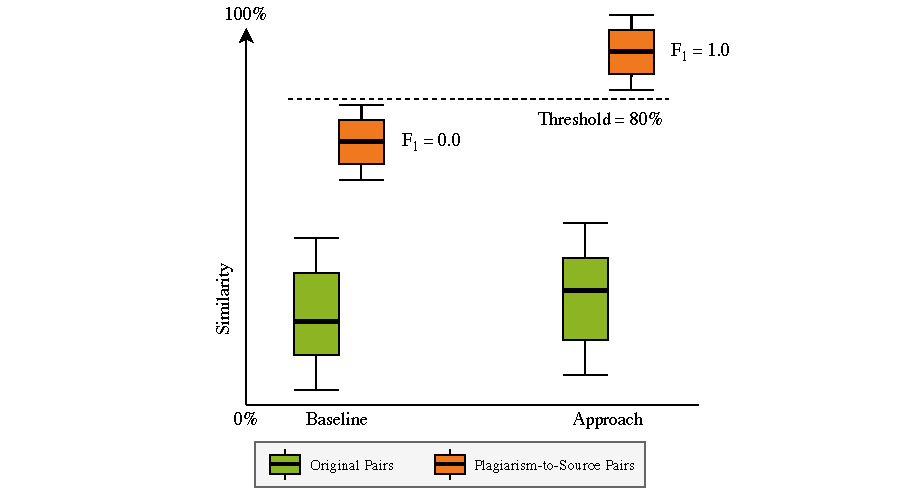
\includegraphics[width=0.95\linewidth]{figures/methodology/Metrics-Thresh.pdf}
    \caption[Problematic Use of Threshold-based Metrics]{Example of threshold-based evaluation where an arbitrary threshold greatly influences the $F_1$ score of an approach and its baseline (note how the shift of original pairs is not considered if below the threshold).}
    \label{fig:diff-threshold-abuse}
\end{figure}

\begin{figure}
    \centering
    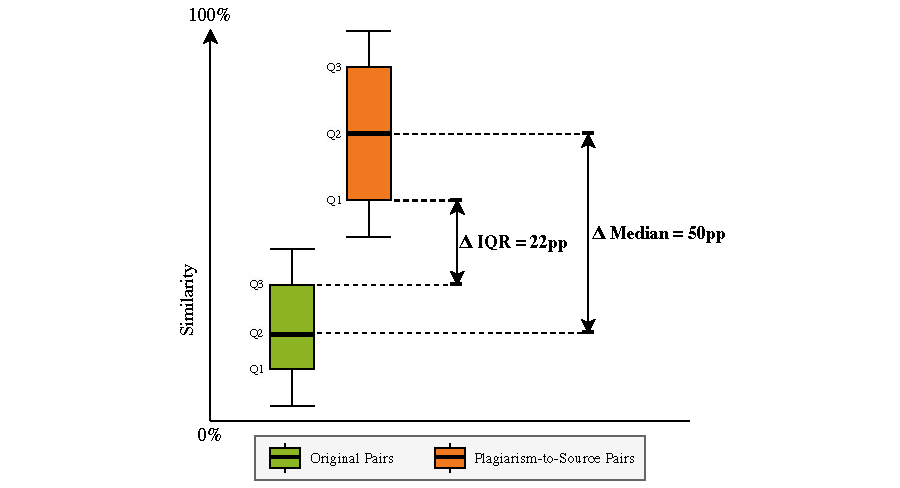
\includegraphics[width=0.95\linewidth]{figures/methodology/DiffMetrics.pdf}
    \caption[Difference Metrics in Plagiarism Evaluations]{Difference metrics comparing the difference between plagiarism instances and original student solutions based on the median and interquartile range (IQR) distances measured in percentage points (as used in our evaluation, see \gqm).}
    \label{fig:diff-metrics}
\end{figure}

Due to these reasons, we instead focus on the magnitude of the difference in similarity values between these types of pairs (as mentioned in our \gqm). The bigger the distance between plagiarism and non-plagiarism pairs, the easier it is to detect plagiarism effectively.
Thus, we measure whether and to \textit{what extent} the considered approaches can find a noticeable difference between these pairs. In contrast to the threshold-based approach and a binary detection metric, we thus employ a magnitude metric.

As each type of pair comprises many similarity scores, different statistical measures can be used to calculate the differences between the types of pairs.
We use measures of central tendency like the mean ($\mu$) or median ($Q_2$) and measures of spread like the difference between the interquartile ranges ($Q_1$ to $Q_3$). For the latter, the difference between the 25th Percentile ($Q_1$) of the plagiarism pairs and the 75th Percentile ($Q_3$) of the unrelated pairs can be measured.

\begin{samepage}
\begin{theorem}[Difference Metrics for Statistical Measures]\label{def:delta-metrics}
Be the \(\mathcal{P}\) the set of all similarity distributions.
Given a distribution of similarity values for plagiarism pairs \(D_p \in \mathcal{P} \) and a distribution of similarity values for unrelated pairs \(D_o \in \mathcal{P}\), we define the following difference metrics \(\mathcal{P} \times \mathcal{P} \rightarrow  \mathbb{Q} \)  to quantify the difference between plagiarism and originals.
%
%We define the interquartile range difference $\Delta IQR$ as
\begin{align*}
    \Delta IQR(D_p, D_o) &= Q_1(D_p) - Q_3(D_o) \\
%
%We define the median difference $\Delta median$ as
    \Delta median(D_p, D_o) &= Q_2(D_p) - Q_2(D_o) \\
%
%We define the median difference $\Delta mean$ as
    \Delta mean(D_p, D_o) &= \mu(D_p) - \mu(D_o) 
\end{align*}
\end{theorem}
\end{samepage}

\autoref{fig:diff-metrics} illustrates an \textbf{example} for the median difference ($\Delta median$) and the distance between interquartile ranges ($\Delta IQR$).
Depending on the choice of statistical measure, a different metric represents different properties of the underlying data. $\Delta median$, for example, is less affected by outliers than $\Delta mean$. The change in IQR ($\Delta IQR$) reflects the degree of separation between most values. When $\Delta IQR$ is greater than zero, at least 75\% of the values in each set do not overlap.
In some cases, outliers can be considered for additional discussions. Outliers are values below the minimum ($Q_1 - 1.5 * IQR$) and above the maximum ($Q_3 + 1.5 * IQR$).

\begin{figure}
    \centering
    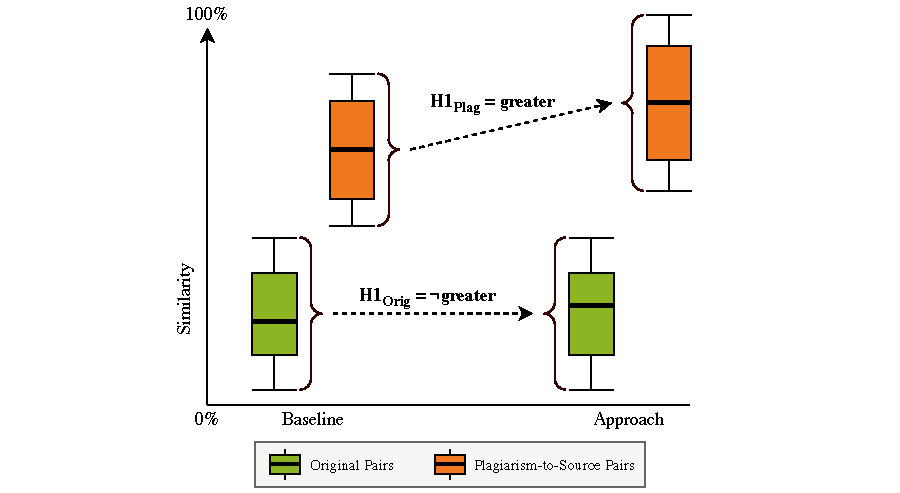
\includegraphics[width=0.95\linewidth]{figures/methodology/SigMetrics.pdf}
    \caption[Statistical Testing in Plagiarism Evaluations]{Visualization of appropriate alternative hypotheses ($H1$) for one-sided significance tests between (paired) plagiarism instances and original student solutions. For plagiarism instances, the location shift should be significantly greater ($H1_{Plag}$); for the originals, the location shift should not be significantly greater ($H1_{Orig}$).}
    \label{fig:sig-metrics}
\end{figure}

Finally, statistical tests can be used, where not only the statistical significance of a result can be assessed, but also the effect size can be used to measure how strong a test result is, thus providing evidence regarding practical significance.
In the case of plagiarism detection, statistical tests can be conducted to compare the significance of a relative improvement in detection quality between the two approaches. 
In this evaluation, we conduct one-sided Wilcoxon signed-rank tests.

Depending on whether the test addresses plagiarism pairs or original shifts, different test hypotheses must be used. \autoref{fig:sig-metrics} illustrates this for both types of pairs. We test the significance regarding a true location shift for the plagiarism pairs, meaning if the plagiarism pairs score significantly higher values (hypothesis $H1_{Plag}$). For the original pairs, it suffices if they remain the same or achieve lesser values (hypothesis $H1_{Orig}$). Thus, we test if the original pairs do \textit{not} have a significant location shift.

For the practical significance, we use \textit{Cliff's delta} $\delta$~\cite{Cliff1993} as an effect size measure, as we typically deal with non-normal distributions when analyzing the similarity distribution of the plagiarism detection system. We do not use \textit{Cohens d}~\cite{Cohen1988}, as it is designed for normal distribution and unpaired data.
While there is a version of \textit{Cohens d} for paired data, it is only robust to small deviations from normality and strongly affected by outliers, which is why it is unsuitable for the typical distributions of plagiarism pair similarities. While \textit{Cliff's delta} $\delta$ is not ideal for paired data, it can still be applied to assess the magnitude of the difference between paired samples, particularly when focusing on rank-based comparisons requiring robustness to non-normality and variance differences.

There are no established categories to interpret the resulting $\delta$ values. Thus, we base our interpretation on the derived categories by \citet{Romano2006} based on \textit{Cohens d}.
Note that these categories are often defined somewhat arbitrarily\footnote{An analogy often used is similarly arbitrary t-shirt sizes. The categories for Cohen's D are used for historical reasons rather than empirical evidence. In practice, interpretations should be based on the specific data and the context of the underlying domain. This is why we combine the indicators for significance with similarity difference metrics.}. We use the following interpretation:
\begin{equation}
    \delta \, \textit{Interpretation}=
    \begin{cases}
        \text{Negligible} & \text{if } 0\ \ \ \ \ \ \ \leq \lvert \delta \rvert < 0.147 \\
        \text{Small} & \text{if } 0.147  \leq \lvert \delta \rvert < 0.33 \\
        \text{Medium} & \text{if } 0.33 \ \ \leq \lvert \delta \rvert < 0.474 \\
        \text{Large} & \text{if } 0.474  \leq \lvert \delta \rvert < 0.7 \\
        \text{Very Large} & \text{if } 0.7 \ \ \ \ \leq \lvert \delta \rvert \leq 1
    \end{cases}
\end{equation}
Note that a negative effect size suggests an adverse interpretation, e.g., that the comparison group is greater than the target group. Nevertheless, due to using absolute values in this equation, the interpretation also applies to negative values.

\section{Choice of Baselines}\label{sec:baselines}
%We chose two separate plagiarism detection approaches as a baseline for our two evaluation goals.
We select two different plagiarism detection approaches as baselines, aligning with our two distinct evaluation goals.

For the evaluation of programming assignments, we utilize JPlag as our baseline. JPlag is not only regarded as a state-of-the-art tool~\cite{Aniceto2021, Novak2019} but also stands out as one of the most frequently referenced approaches and the most compared approach in the literature~\cite{Novak2019}. Its widespread use in practice and scientific literature makes it an ideal standard for assessing programming-based plagiarism.

While MOSS is also widely used and well~\cite{Novak2019}, we decided not to use it as a baseline for four reasons. First, MOSS does not return all similarity values but only a subset of the highest scores, which skews the results and thus hinders a fair comparison of plagiarism instances with unrelated programs. Second, MOSS is closed-source, making it difficult to extend with the defense mechanisms required for a direct comparison. Third, MOSS can only be used by sending the datasets to its server at Stanford in the United States. Thus, we could not have used internal datasets due to \ac{GDPR} concerns. Finally, MOSS severely limits how frequently its service can be used, thus making it infeasible for larger evaluations.
Likewise, we excluded Dolos as a baseline, as it is relatively recent, less widely used, and only supports single-file programs, which limits its applicability for many of the datasets we use for evaluation. Programs that consist of multiple files are common in programming assignments, and thus, it is important to evaluate based on such datasets.
%
Both MOSS and Dolos, however, are token-based and thus conceptually very similar to JPlag.
Importantly, they are also equally vulnerable to obfuscation attacks~\cite{DevoreMcDonald2020, Saglam2024c}, reinforcing the necessity of improvement via defense strategies. 

\begin{figure}[b]
    \centering
    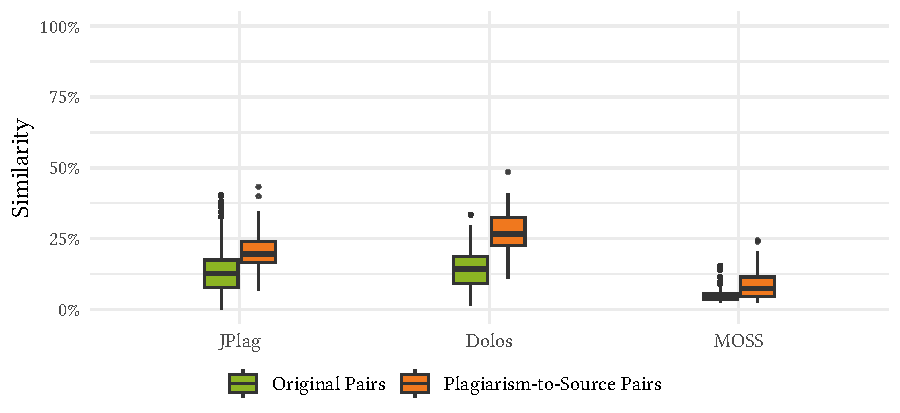
\includegraphics[width=0.99\linewidth]{figures/methodology/vulnerability_avg.similarity.pdf}
    \caption[Obfuscation Vulnerability of Different Detection Systems]{Obfuscation vulnerability illustrated for the three token-based approaches JPlag, Dolos, and MOSS with the dataset PROGpedia-19~\cite{paiva2023} and plagiarism instances automatically obfuscated via statement insertion.}
    \label{fig:vuln}
\end{figure}

As an example, \autoref{fig:vuln} illustrates the performance of JPlag, MOSS, and Dolos for a simple programming dataset and insertion- and reordering-based obfuscation attacks.
All three approaches compute only low similarities for the plagiarism instances, which thus overlap with unrelated original programs.
Note that many of the lower similarity values were omitted for MOSS as it does not provide them. Furthermore, the dataset used here consists only of small, single-file programs that are compatible with Dolos.

For the evaluation with modeling assignments, we adopt the \ac{LSH} approach developed by \citet{Martinez2020} as our baseline. To the best of our knowledge, this is the only existing plagiarism detection approach designed specifically for modeling artifacts. Given that the detection of plagiarism in modeling assignments presents unique challenges, their approach provides a suitable comparison point.
%
The token-based plagiarism detection for modeling artifacts, which is part of \contribution{2}, was implemented based on JPlag, as it is, compared to MOSS, open-source, and also because it is considered a state-of-the-art tool~\cite{Novak2019, weber2012, Aniceto2021}. Thus, it is considered the approach and not a baseline; thus, we use the approach of \citet{Martinez2020} as a baseline to evaluate our contributions.

In summary, we use state-of-the-art approaches as a baseline for evaluation and can thus show that our contributions outperform the state-of-the-art.


\section{Datasets}\label{sec:datasets}
Evaluating software plagiarism detection systems requires diverse datasets to capture various aspects of student submissions across different programming and modeling tasks. These datasets typically fall into two categories: public datasets, which are accessible to the research community, and private datasets, which are often proprietary or cannot be published due to data protection laws such as the \ac{GDPR} of the European Union. Public datasets provide a common ground for comparison across studies but are often limited in size and quality. 
%
The following subsections list several datasets used in our evaluation, covering both programming and modeling assignments. The selected datasets vary in size, programming languages, and types of tasks, offering a comprehensive basis for evaluating our contributions. 

\subsection{Programming Assignment Datasets}
There are some public datasets from real university courses for programming assignments. Some of them, meant for evaluating plagiarism or clone detection approaches, even contain plagiarism instances.
However, most of these datasets have one more issue. Often, they contain many invalid programs or (near) empty programs. Furthermore, if they contain plagiarism, there often is no labeling available. And even if there are labels, they are often incomplete, as obvious verbatim copies are not included. Another issue is the source of the labels. Often, it is a mix of manual labeling assisted by JPlag or MOSS, as they are considered state-of-the-art\footnote{Amusingly, this is a challenge when trying to evaluate JPlag with public datasets. The labels are often created with JPlag, thus defeating the purpose of using them in an evaluation.}.
These issues, however, can be addressed via careful preprocessing.
When evaluating automated obfuscation, the existing (human) plagiarism instances need to be filtered out first, which is challenging if the labeling is incomplete, or no labels are provided at all.
%
The size of these public datasets, however, cannot be addressed via preprocessing. They often contain a limited number of (valid) programs. Furthermore, most of these programs are very small and thus not representative of larger assignments.

To address these issues, we combine public with internal datasets and carefully preprocess the public datasets.
We used a total of six real-world datasets; four are publicly available, and two are internal. They all come from an educational setting but stem from different courses and assignment types.
Thus, they vary in the number and size of the programs, but especially in their programming language.
First, we used two tasks from the publicly available collection \textit{PROGpedia}~\cite{paiva2023}.
Here, Task 19 covers the design of a graph data structure and a depth-first search to analyze a social network.
Task 56 concerns minimum spanning trees using Prim's algorithm. Both datasets contain small Java programs.
For both datasets, we used only syntactically and semantically correct solutions and the latest version of each program.

Next, we used the \textit{TicTacToe} dataset~\cite{Saglam2024b}, which contains command-line-based Java implementations of the paper-and-pencil game TicTacToe. 
This dataset is from an introductory programming class at KIT, specifically from a weekly assignment.
This dataset contains many programs, each of which is medium-sized.
%We removed all instances of human plagiarism and programs with suspiciously high similarity.
We also used the \textit{BoardGame} dataset~\cite{Saglam2024b}. This assignment is from the same course as the \textit{TicTacToe} dataset. However, it is the final project of the course. Here, the task is also a command-line-based game; however, this time, it is a comprehensive board game. Thus, it contains very large programs, which are at the upper end for a typical program in software plagiarism detection (see \autoref{sec:survey}).
%This dataset did not contain any plagiarism cases.

Finally, we used two tasks from the publicly available homework dataset by \citet{Ljubovic2020a}.
While both tasks contain C++ programs, one pertains to managing student and laptop records within a university setting, whereas the other requires implementing a Fourier series.
To prepare the datasets for our evaluation, we removed all solutions that did not compile, as JPlag requires valid input programs.
We also removed all human plagiarism (if present) based on the labeling provided by the datasets. If no labeling was present, we removed verbatim copies.
This notably reduces the size of some datasets.
%&Thus, we ended up with the following five datasets (size is measured in lines of code (LOC), excluding comments and empty lines):
Consequently, we obtained the six datasets listed in \autoref{tab:prog-datasets}.

\begin{table}[b]
    \centering
    \begin{tabular}{lrrrr}
        \toprule
        {Dataset Name} & {\# Programs} & {Mean LOC} & Language & Source \\
        \midrule
        PROGpedia Task 19 & 27 & 131 & Java & \cite{paiva2023}\\
        PROGpedia Task 56 & 28 & 85 & Java & \cite{paiva2023}\\
        TicTacToe & 626 & 236 & Java & \scriptsize{internal}\\
        BoardGame & 434 & 1529 & Java & \scriptsize{internal}\\
        Homework Task 1 & 59 & 282 & C/C++ & \cite{Ljubovic2020a}\\
        Homework Task 5 & 18 & 123 & C/C++ & \cite{Ljubovic2020a}\\
        \bottomrule
    \end{tabular}
    \caption[Evaluation Datasets]{Overview of the programming assignment datasets used for the evaluation with the number of included programs, mean size in lines of code (LOC) excluding comments and empty lines, the programming language, and source of the dataset.}
    \label{tab:prog-datasets}
\end{table}

\subsection{Modeling Assignment Datasets}\label{sec:datasets-mde}
While public datasets are available for programming assignments, albeit with varying quality, this is not the case for modeling assignments.
Artificially constructed datasets offer control over scale, but they lack realism and are, therefore, not a good option either.
Thus, we use an internal dataset~\cite{Saglam2022} from a \textit{typical}~\cite{Ciccozzi2018} modeling assignment.
This data set contains 21 metamodels from modeling assignments from a master's level elective practical course on model-driven software development.
These 21 metamodels are, to the best of our knowledge, free of plagiarism\footnote{As this is a master's level elective course and the students work in groups anyway, there is not much incentive for plagiarism. However, we carefully inspected the solutions on plagiarism to make sure they are free of plagiarism.}.
%Thus, the dataset provides 210 pairs of original, student-made solutions.

The assignment tasks the students in groups of two to five to create a metamodel for designing component-based system architectures. This metamodel can be used to create models similar to \ac{UML} component diagrams but also involves additional aspects, such as software-to-hardware allocation.
A component-based system can be designed using four different view types: A component repository, the component assembly, the environment, and the allocation.
The \textit{repository} manages all components and interfaces that may be reused within multiple systems. The \textit{assembly} shows how components are instantiated and interconnected. The \textit{environment} depicts all containers and the links between them. The \textit{allocation} specifies which components of the assembly are allocated on which containers of the environment.
This assignment is loosely based on the Palladio component model~(PCM)~\cite{reussner2016a, becker2008a}.

On average, a student solution for the assignment contains five packages, 39 classifiers, 45 references, ten attributes, and one operation.
While most student solutions were designed in a single file, some students fragmented them into several files.
%
The dataset serves as a set of original, unrelated solutions for the first and third evaluation goals related to modeling assignments. 
The pairwise comparison of 21 submissions yields 210 pairs, i.e., $\binom{21}{2}=210$, which are false positives when detected as plagiarism.


% ----------------- Part 2 -----------------  %
\chapter[Evaluating Obfuscation Resilience]{Evaluating Obfuscation Resilience for Programming Assignments}\label{cha:code-eval}

In this chapter, we evaluate our defense mechanisms against automated obfuscation attacks (\contribution{3}) with datasets from real-world programming assignments. Thus, this chapter addresses our first evaluation goal (\gref{1}).
This evaluation stage thus shows that our defense mechanisms provide obfuscation resilience against all categories of the obfuscation attack classification discussed in our threat model (see \autoref{sec:threatmodel-categorization}). Note that this stage only includes the defense mechanisms that apply to programming languages, namely token sequence normalization, subsequence match merging, and the combination of both. The evaluation for modeling languages follows in the second evaluation stage.
In this evaluation stage, we use JPlag as a baseline, as it is state-of-the-art for programming assignments.
%
The evaluation is based on six real-world datasets, totaling 758 original and 968 automatically obfuscated programs.
In sum, these programs consist of over 14,000 files and close to one million lines of code.
%This yields a total of 289,046 pairwise comparisons.
We provide a replication package~\fancycite{replication-package}.

Our results demonstrate that our defense mechanisms offer broad obfuscation resilience across diverse datasets and attack types, thus significantly advancing resilience against automated obfuscation attacks.
%
Notably, we achieved a median similarity difference increase of up to 99.65 percentage points against semantic-preserving insertion-based obfuscation. We also show substantial improvements against alteration-based attacks (up to 42 percentage points) and refactoring-based attacks (up to 22 percentage points). While resilience against AI-based obfuscation was comparatively lower (up to 19 percentage points), we still effectively improved detection rates, including a notable 6.5 percentage point increase in identifying AI-generated programs despite the fact that the defense mechanisms are not designed for this use case.

The remainder of the chapter is structured as follows:
First, we introduce the obfuscation attacks used in the evaluation and how we applied them to the datasets to generate the plagiarism instances.
Second, we present the detailed results for each attack type individually, highlighting the impact of our defense mechanisms.
Next, we present a brief summary of the most important results.
This is followed by a discussion section, where we interpret the results and discuss takeaways for software plagiarism detection.
Finally, we address potential threats to validity and how we addressed them, for example, factors that influence the generalizability of the results.

\ownpublications{
    \fancycite{Saglam2024b} and
    \fancycite{Saglam2024d}.
}

\section{Obfuscation Attacks}
To answer the questions regarding our first evaluation goal, we employ five different types of automated obfuscation attacks, three of which are algorithmic and two AI-based.
In the following, we will briefly discuss these obfuscation attacks\footnote{Note that for ethical reasons, we do not discuss details of the obfuscation attack. We do not want to encourage the use of these attacks. Thus, we purposefully omit details.}.
The algorithmic obfuscation attacks are statement insertion, refactoring, and simulated random alteration.
For the AI-based ones, we employ AI-based obfuscation and full generation from the assignment description via large language models.
Note that we do not evaluate reordering-based obfuscation, as it is a very weak obfuscation attack for source code.
The interested reader can find an evaluation for such obfuscation in \fancycite{Saglam2024b}.
 
The first algorithmic obfuscation attack is the insertion of dead statements.
For this, we employ two different tools. The first one is \mossad~\cite{DevoreMcDonald2020}. As previously discussed, it is indeterministic and operates threshold-based. The second is \textit{PlagGen}~\cite{Broedel2023}, which is similar to \mossad but is deterministic and exhaustive (see \autoref{sec:threatmodel-automation}). In both cases, the statement insertion uses statements from the original program and a pool of pre-defined statements. Furthermore, both ensure that the inserted statements do not change the behavior of the programs. Thus, this obfuscation attack is semantic-preserving. We use PlagGen for Java and \mossad for C++, as these are the languages supported by each tool.
%
Second, we employ the refactoring-based obfuscation attack by \citet{Maisch2024}, which leverages \textit{Spoon}~\cite{Pawlak2006} automatically applies semantic-preserving refactoring operations at random positions at the AST-level to obfuscate a program.
In detail, the refactoring operations include optional wrapping, extracting expressions as new variables, introduction of constant container classes and extraction of constants, swapping of if-else-statements and inverting the corresponding conditions, insertion of methods and constructors, and the introduction of access methods for existing fields.
As the behavior of the programs is not changed, this obfuscation attack is also semantic preserving.
This implementation of the obfuscation attack only supports Java programs, so we only use four of the six datasets with this obfuscation attack.
%
Third, we simulate a semantic-agnostic obfuscation attack by randomly changing 25\% of the tokens to a different one. While this attack is only simulated, it mirrors the effects of strong obfuscation attempts that alter a quarter of the program's code \textit{without} considering program behavior. This obfuscation attack simulates strong obfuscation or partial re-implementation.

For the AI-based obfuscation attacks, we exploit OpenAI's GPT-4 for automated plagiarism, which is currently the state-of-the-art LLM.
There are generally two ways of using generative AI to \textit{cheat} for programming assignments (see \autoref{sec:threatmodel-automation}):
\textit{AI-based obfuscation}, where the adversary provides an AI model with a pre-existing program and tasks it to generate an obfuscated version.
\textit{AI-based generation}, where the adversary uses the assignment's description to generate a program from scratch via an AI model.
%
We employ AI-based obfuscation as a third obfuscation attack alongside both algorithmic ones. We use fifteen different prompts, mimicking how students would ask GPT to obfuscate their plagiarism.
The prompts range from requesting minor structural changes to requesting a reimplemented version of the original program. As for this attack, the programs need to be sent to the OpenAI GPT server; we did not use it for the BoardGame dataset due to its sensitive nature.
Finally, we use full generation as the final obfuscation. However, we can only employ it for the TicTacToe dataset, as we require the full assignment description and test cases to test for the expected behavior.
AI-based obfuscation is a semantic agnostic attack. While the prompts contain instructions to preserve the program behavior, there are generally no guarantees that the changes proposed by GPT-4 conform to these instructions. 
Similarly, for AI-based generation, there is no guarantee that the programs fully implement all details requested by the task.
%%%%%%%
In sum, we use the following four techniques attacks to create 787 plagiarized programs (see \autoref{tab:plagiate} for details):
\begin{enumerate}[noitemsep]
 \item \textbf{Insertion-based Obfuscation} (semantic-preserving): Inserting new and existing statements into the program (PlagGen~\cite{Broedel2023} for Java and \mossad~\cite{DevoreMcDonald2020} for C/C++).
 \item \textbf{Refactoring-based Obfuscation} (semantic-preserving): Applying a variety of semantic-preserving refactoring operations, for example, transformations of control structures, field access, and method granularity~\cite{Maisch2024}.
 \item \textbf{Alteration-based Obfuscation} (semantic-agnostic): Simulate changing large parts of the program by randomly changing 25\% of the tokens to different tokens.
 \item \textbf{AI-based Obfuscation} (sematic-agnostic): We obfuscate human solutions with GPT-4~\cite{gpt4} based on 15 varying prompts requesting structural changes.
 \item \textbf{AI-based Generation} (sematic-agnostic): We fully generate AI-based solutions with GPT-4~\cite{gpt4} based on only the textual task description of the assignment.
\end{enumerate}
%
According to the threat categorization in \autoref{fig:clone-types}, semantic-preserving obfuscation using insertion is categorized as a structural attack. Semantic-agnostic obfuscation simulates structural and complex attacks but refactoring only to a lesser extent. AI-based obfuscation is multifaceted, mapping to both structural and complex attacks, particularly refactoring attacks. AI-based generation is classified as full re-implementation, which is highly challenging to address. Our evaluation, therefore, systematically covers the broad range of possible obfuscation attacks. While our defense mechanisms are mainly designed for semantic-preserving obfuscation attacks, we also evaluate with semantic-agnostic ones.
%
However, focusing solely on the attacks on a program level overlooks the broader principle that all obfuscation attacks, regardless of their type, must ultimately affect the token sequences (see \autoref{sec:threatmodel-analysis}). Thus, our evaluation covers a wide range of attack types.
%
\begin{table}[b]
	\centering
    \small
    \setlength{\tabcolsep}{5pt}
	\begin{tabular}{lcccccc}
		\toprule
		Obfuscation Attack Type  & PROGp.-19 & PROGp. & Homew.-1 & Homew.-5 & TTT & BoardGame\\
		%Type                     & PROGpedia-19 & PROGpedia-56 & Homework-1 & Homework-5 & TicTacToe \\
		\midrule
		Insertion-based Obf. & 27    & 28    & 59   & 17   & 50 & 20 \\
		Alteration-based Obf.   & 27    & 28    & 59   & 17   & 50 & 20 \\
        Refactoring-based Obf.   & 27    & 28    & -   & -  & 50 & 20 \\
		AI-based Obf. & 75    & 75    & 75   & 75   & 75 & - \\
		AI-based Generation      & -     & -     & -    & -    & 50 & -\\
		\bottomrule
	\end{tabular}
    \caption[Obfuscation Attacks]{Overview on the number of plagiarized programs per dataset and obfuscation attack type (952 in total). Each of the 15 prompts is applied to 5 originals for the AI-based obfuscation.}
    \label{tab:plagiate}
\end{table}
%\todo{(MEDIUM) update and expand. Emphasis on systematically covering the classes and that the type corresponds to the questions of goal 1.}

\section{Result Analysis}

This section presents the evaluation results for our defense mechanisms, demonstrating that they significantly improve resilience against all five obfuscation attack types. As these obfuscation attack types systematically cover the categories presented in \autoref{fig:clone-types}, we provide broad resilience against automated obfuscation attacks.

In the following, we will discuss the results of each obfuscation attack type \textit{individually}. As using different obfuscation attacks only affects the plagiarism instances, the unrelated programs of each dataset remain the same for all evaluation stages. Thus, we first discuss the effect of our defense mechanism on unrelated programs.

As discussed in \autoref{fig:clone-types}, we illustrate the results via boxplots, calculate difference metrics for selected statistical measures, and conduct statistical tests to analyze statistical and practical significance. As this is done for each of the five obfuscation attack types and the baseline for each of the applicable datasets, as well as for the baseline, TSN, SMM, and the combination of the former two, we conduct a total of 72 statistical tests and calculate 228 difference values.

The interplay of multiple obfuscation techniques, datasets, and defense mechanisms, combined with the sheer number of statistical comparisons, naturally contributes to the complexity of the results. Despite this inherent complexity, we made every effort to present them in a manner that is as straightforward as possible. 
However, this complexity reflects the rigor of the analysis, which is essential to fully assess the effectiveness of the proposed defense mechanisms.

%\todo{maybe add a high-level summary of results}

% ------------------------------------------------------- $
\begin{table}
\centering
\small
\begin{tabular}{lrrrrrrrr}
  \toprule
ds & Variant & Pairs & $p$ & $W$ & $\delta$ & $\delta\,Int.$ & $\delta$ 95\% CI & n \\ 
  \midrule
    \multirow{3}{*}{\rotatebox[origin=c]{90}{Pp.-19}} & TSN & OP & 8.3e-05 & 13,137 & 0.005 & Negligible & [-0.08, 0.09] & 351 \\ 
   & SMM & OP & < 1e-10 & 6,441 & 0.178 & Small & [0.09, 0.26] & 351 \\ 
   & Both & OP & < 1e-10 & 26,133 & 0.185 & Small & [0.10, 0.27] & 351 \\ 
   \hline
  \multirow{3}{*}{\rotatebox[origin=c]{90}{Pp.-56}} & TSN & OP & 0.25 & 3,580 & -0.034 & Negligible & [-0.11, 0.04] & 378 \\ 
   & SMM & OP & < 1e-10 & 4,753 & 0.154 & Small & [0.08, 0.23] & 378 \\ 
   & Both & OP & < 1e-10 & 14,018 & 0.148 & Negligible & [0.07, 0.22] & 378 \\ 
  \hline
   \multirow{3}{*}{\rotatebox[origin=c]{90}{TTT}} & TSN & OP & < 1e-10 & 1,256,914,634 & 0.009 & Negligible & [0.01, 0.01] & 188,805 \\ 
   & SMM & OP & < 1e-10 & 3,346,969,836 & 0.177 & Small & [0.17, 0.18] & 188,805 \\ 
   & Both & OP & < 1e-10 & 6,099,071,135 & 0.186 & Small & [0.18, 0.19] & 188,805 \\ 
   \hline
  \multirow{3}{*}{\rotatebox[origin=c]{90}{BG}} & TSN & OP & < 1e-10 & 1,379,905,112 & 0.021 & Negligible & [0.01, 0.03] & 67,161 \\ 
   & SMM & OP & < 1e-10 & 1,637,665,065 & 0.104 & Negligible & [0.10, 0.11] & 67,161 \\ 
   & Both & OP & < 1e-10 & 2,069,412,722 & 0.124 & Negligible & [0.12, 0.13] & 67,161 \\ 
   \hline
  \multirow{3}{*}{\rotatebox[origin=c]{90}{Hw.-1}} & TSN & OP & 1 & 378,825 & -0.069 & Negligible & [-0.11, -0.03] & 1,711 \\ 
   & SMM & OP & < 1e-10 & 557,040 & 0.161 & Small & [0.12, 0.20] & 1,711 \\ 
   & Both & OP & < 1e-10 & 656,971 & 0.106 & Negligible & [0.07, 0.14] & 1,711 \\ 
   \hline
  \multirow{3}{*}{\rotatebox[origin=c]{90}{Hw.-5}} & TSN & OP & 0.58 & 2,229 & -0.058 & Negligible & [-0.19, 0.07] & 153 \\ 
   & SMM & OP & 3.9e-10 & 1,275 & 0.111 & Negligible & [-0.02, 0.24] & 153 \\ 
   & Both & OP & 0.015 & 3,153 & 0.062 & Negligible & [-0.07, 0.19] & 153 \\ 
   \bottomrule
\end{tabular}
\caption[Statistical Tests: Unrelated Pairs]{One-sided Wilcoxon signed-rank test results for \textbf{unrelated, student-made programs} regarding the potential adverse effects of our defense mechanisms compared to the baseline (sig. level of $\alpha=0.01$, alternative hypothesis $H1=greater$, test statistic $W$, effect size via Cliff's delta $\delta$, its interpretation $\delta\,Int.$, its 95 percent confidence interval $CI$, and the sample size $n$). Note that for original pairs (OP), high $p$ and low $\delta$ are desirable, as original pairs should \textit{not} be $greater$.} 
\label{tab:to-base-original}
\end{table}
 
% ------------------------------------------------------- $

\subsection{Effect on Unrelated Programs}\label{sec:eval-unrel}
To achieve a high separation between plagiarism instances and unrelated programs, it is not only important to achieve high similarity values for the plagiarism pairs.
It is also essential to affect the pairs of unrelated, original programs made by students as little as possible. 
Our results show that the effect on unrelated programs in our evaluation is insignificant. This means the false-positive rate did not significantly increase.
\autoref{tab:to-base-original} shows the results of the statistical tests for the original pairs. We test if the defense mechanisms significantly increase similarity values for the original pairs compared to the baseline.

Token sequence normalization has virtually no effect on unrelated programs.
For all but one dataset, the median similarity values of the original pairs increase by between 0.00 (PROGpedia-56) and 0.28 (Homework-5) percentage points.
For the other dataset, namely Homework-1, the median similarity values \textit{decrease} by 1.23 percentage points. This means that for this dataset, token sequence normalization reduces the similarity of programs that were implemented unrelated to each other.
The statistical tests show that these changes in similarity values are not statistically significant for five of the six datasets. The change is statistically significant for the PROGpedia-19 dataset. However, the change is not practically significant, as the effect size for all datasets is \textit{negligible}.
%
Subsequence match merging has a small but insignificant effect on unrelated programs. This can be explained by the heuristic nature of the defense mechanism.
For all datasets, the median similarity values of the original pairs increase by between 0.78 (BoardGame) and 6.59 (PROGpedia-56) percentage points.
While the statistical tests show that these changes in similarity values are indeed statistically significant for four of the six datasets, the effect sizes for all six datasets are \textit{negligible} to \textit{small}.
Thus, the effect on the unrelated programs has little to no practical significance. 

When both defense mechanisms are combined, the effects are similar to subsequence match merging on its own.
For all datasets, the median similarity values of the original pairs increase by between 0.91 (BoardGame) and 6.75 (PROGpedia-19) percentage points.
Again, these changes are statistically significant for three of the six datasets but have little to no practical significance, as the effect sizes are \textit{negligible} for four datasets and \textit{small} for the two remaining (PROGpedia-19 and TicTacToe).

\summaryBox{1.1}{The effect of our defense mechanisms on unrelated programs, and thus the potential impact on the false positive rate, is negligible and, therefore, practically insignificant and, in some cases, even statistically insignificant.}

\subsection{Insertion-based Obfuscation}\label{sec:eval-insert}
% FIGURE TEXT
\autoref{fig:stage1-results} shows the results for obfuscation attacks based on inserting statements into plagiarized programs.
\autoref{tab:diff-insert} shows the corresponding statistical measures.
% ATTACK TYPE REFRESHER TEXT
As discussed previously, we use \mossad~\cite{DevoreMcDonald2020} for the C++-based datasets Homework-1 and Homework-5. For all others, we use PlagGen~\cite{Broedel2023}. Note that the main difference between both plagiarism generators is the termination criterion, as \mossad operates threshold-based while PlagGen employs an exhaustive strategy.

Note that there is a disparity between the token sequence normalization implementation between Java and C++\footnote{This concerns the step of adding semantic information to the token sequence, which is the only part of token sequence normalization that is not language-independent.}.
It stems from the complex nature of C++, which includes substantial undefined behavior and highly expressive syntax, which raises the engineering effort required to address all edge cases effectively. However, this limitation is purely technical.

\begin{table}[h]
	\centering
	\small
	\begin{tabular}{lrrrrrrrr}
		\toprule
		Dataset                       & Variant & Median     & Mean      & $Q_1$      & $Q_3$      & $\Delta$ Mean & $\Delta$ Median & $\Delta$ IQR \\
		\midrule
		\multirow{4}{*}{PROGpedia-19} & Base     & 10.61      & 11.10     & 8.17       & 12.67      & 5.37          & 5.55            & -0.74        \\ 
		                              & TSN      & \B{100.00} & \B{99.87} & \B{100.00} & \B{100.00} & \B{94.12}     & \B{94.87}       & \B{91.06}    \\ 
		                              & SMM      & 35.10      & 37.12     & 28.36      & 47.94      & 27.97         & 28.74           & 15.16        \\ 
		                              & Both     & \B{100.00} & \B{99.87} & \B{100.00} & \B{100.00} & 90.66         & 93.43           & 86.12        \\ 
		\hline
		\multirow{4}{*}{PROGpedia-56} & Base     & 19.59      & 21.36     & 14.86      & 25.33      & 16.47         & 19.59           & 6.09         \\ 
		                              & TSN      & \B{99.65}  & \B{99.66} & \B{99.47}  & \B{100.00} & \B{95.14}     & \B{99.65}       & \B{90.82}    \\ 
		                              & SMM      & 58.08      & 56.70     & 47.75      & 62.91      & 48.44         & 51.49           & 35.56        \\ 
		                              & Both     & \B{99.65}  & \B{99.66} & \B{99.47}  & \B{100.00} & 91.54         & 92.91           & 86.85        \\ 
		\hline
		\multirow{4}{*}{TicTacToe}    & Base     & 5.29       & 6.36      & 2.57       & 9.66       & -0.49         & -0.78           & -7.39        \\ 
		                              & TSN      & \B{99.52}  & \B{99.42} & \B{99.18}  & \B{100.00} & \B{92.48}     & \B{93.37}       & \B{89.11}    \\ 
		                              & SMM      & 22.36      & 23.39     & 13.01      & 31.14      & 14.57         & 14.52           & 0.49         \\ 
		                              & Both     & \B{99.52}  & \B{99.42} & \B{99.18}  & \B{100.00} & 90.49         & 91.58           & 86.54        \\
        \hline
		\multirow{4}{*}{BoardGame}    & Base     & 18.72      & 18.66     & 15.49      & 22.85      & 2.48          & 2.53            & -3.49        \\ 
		                              & TSN      & \B{97.23}  & \B{96.82} & \B{95.82}  & \B{98.07}  & \B{80.49}     & \B{80.90}       & \B{76.69}    \\ 
		                              & SMM      & 24.97      & 24.12     & 20.81      & 28.65      & 7.18          & 8.01            & 1.06         \\ 
		                              & Both     & \B{97.23}  & \B{96.82} & \B{95.82}  & \B{98.07}  & 79.72         & 80.13           & 75.92        \\
		\hline
		\multirow{4}{*}{Homework-1}   & Base     & 19.45      & 18.36     & 18.86      & 19.90      & 7.97          & 9.57            & 3.27         \\ 
    		                           & TSN      & 42.83      & 43.58     & 36.57      & 49.84      & 34.21         & 34.19           & 22.92        \\ 
		                               & SMM      & 38.57      & 40.63     & 34.75      & 43.63      & 27.58         & 25.99           & 15.25        \\ 
		                               & Both     & \textbf{74.10}      & \textbf{73.32}     & \textbf{65.88}      & \textbf{80.09}      & \textbf{61.32}         & \textbf{62.48}           & \textbf{48.45}        \\ 
		\hline
		\multirow{4}{*}{Homework-5}   & Base     & 19.24      & 19.38     & 19.03      & 19.91      & 5.99          & 7.25            & -0.65        \\ 
		                               & TSN      & 38.63      & 42.05     & 30.90      & 58.65      & 30.39         & 26.36           & 15.06        \\ 
		                               & SMM      & 40.89      & 43.36     & 30.05      & 54.77      & 27.44         & 26.91           & 6.40         \\ 
		                               & Both     & \textbf{74.57}      & \textbf{75.21}     & \textbf{59.98}      & \textbf{93.46}      & \textbf{60.62}         & \textbf{61.22}           & \textbf{40.40}        \\  
		\bottomrule  
	\end{tabular}
	\caption[Evaluation Results: Insertion-based Obfuscation]{Statistical measures for plagiarism pairs and their differences ($\Delta$) from original pairs for \textbf{insertion-based obfuscation} (corresponds to \autoref{fig:stage1-results}). Higher values indicate better performance. Note that measures are expressed as percentages and their differences as percentage points.}
	\label{tab:diff-insert}
\end{table}



% ------------------------------------------------------- $
\begin{table}[h]
	\centering
	\small
	\begin{tabular}{lrrrrrrrr}
		\toprule
		ds                              & Variant & Pairs & $p$     & $W$   & $\delta$ & $\delta\,Int.$ & $\delta$ 95\% CI & n  \\ 
		\midrule
		\multirow{3}{*}{{PROGpedia-19}} & TSN     & P2S   & 3e-06   & 378   & 1.000    & Very Large     & [1.00, 1.00]     & 27 \\ 
		                                & SMM     & P2S   & 3e-06   & 378   & 0.904    & Very Large     & [0.70, 0.97]     & 27 \\ 
		                                & Both    & P2S   & 3e-06   & 378   & 1.000    & Very Large     & [1.00, 1.00]     & 27 \\ 
		\hline
		\multirow{3}{*}{{PROGpedia-56}} & TSN     & P2S   & 2e-06   & 406   & 1.000    & Very Large     & [1.00, 1.00]     & 28 \\ 
		                                & SMM     & P2S   & 2e-06   & 406   & 0.939    & Very Large     & [0.79, 0.98]     & 28 \\ 
		                                & Both    & P2S   & 2e-06   & 406   & 1.000    & Very Large     & [1.00, 1.00]     & 28 \\ 
        \hline
		\multirow{3}{*}{{TicTacToe}}    & TSN     & P2S   & 3.9e-10 & 1,275 & 1.000    & Very Large     & [1.00, 1.00]     & 50 \\ 
		                                & SMM     & P2S   & 8.4e-10 & 1,176 & 0.766    & Very Large     & [0.60, 0.87]     & 50 \\ 
		                                & Both    & P2S   & 3.9e-10 & 1,275 & 1.000    & Very Large     & [1.00, 1.00]     & 50 \\ 
        \hline
		\multirow{3}{*}{{BoardGame}}    & TSN     & P2S   & 4.8e-05 & 210   & 1.000    & Very Large     & [1.00, 1.00]     & 20 \\ 
		                                & SMM     & P2S   & 4.8e-05 & 210   & 0.545    & Large          & [0.20, 0.77]     & 20 \\ 
		                                & Both    & P2S   & 4.8e-05 & 210   & 1.000    & Very Large     & [1.00, 1.00]     & 20 \\ 
		\hline
		\multirow{3}{*}{{Homework-1}}   & TSN     & P2S   & < 1e-10 & 1,770 & 1.000    & Very Large     & [1.00, 1.00]     & 59 \\ 
		                                & SMM     & P2S   & < 1e-10 & 1,653 & 0.955    & Very Large     & [0.82, 0.99]     & 59 \\ 
		                                & Both    & P2S   & < 1e-10 & 1,770 & 1.000    & Very Large     & [1.00, 1.00]     & 59 \\  
		\hline
		\multirow{3}{*}{{Homework-5}}   & TSN     & P2S   & 1.3e-4  & 170   & 0.889    & Very Large     & [0.45, 0.98]     & 18 \\ 
		                                & SMM     & P2S   & 1.6e-4  & 153   & 0.969    & Very Large     & [0.83, 0.99]     & 18 \\ 
		                                & Both    & P2S   & 1.1e-4  & 171   & 1.000    & Very Large     & [0.99, 1.00]     & 18 \\ 
		\bottomrule
	\end{tabular}
	\caption[Statistical Tests: Insertion-based Obfuscation]{One-sided Wilcoxon signed-rank test results for \textbf{insertion-based obfuscation} regarding the improvement by our defense mechanism compared to baseline (sig. level of $\alpha=0.01$, alternative hypothesis $H1=greater$, test statistic $W$, effect size via Cliff's delta $\delta$, its interpretation $\delta\,Int.$, its 95 percent confidence interval $CI$, and the sample size $n$). For plagiarism-to-source pairs (P2S), low $p$ and high $\delta$ are desirable.} 
	\label{tab:to-base-insert}
\end{table}
 
% ------------------------------------------------------- $

%\multirow{3}{*}{Effects of Normalization} 

\subsubsection{Baseline}
\autoref{fig:stage1-results} illustrates the drastic impact of insertion-based obfuscation attack on the baseline.
For the baseline, the median similarity values for plagiarism pairs (true positives) drop to between 5.29 percent (TicTacToe) and 19.59 percent (PROGpedia-56), depending on the dataset.
This results in a complete overlap between plagiarism and original pairs for all datasets except PROGpedia-56. Here, however, we can still observe a substantial overlap.

Notably, we observe that for the TicTacToe dataset, the median similarity values for the plagiarism pairs are \textit{lower} than for the original pairs.
As shown in \autoref{tab:diff-insert}, the median similarity \textit{differences} between plagiarism and original pairs range from -0.78 percentage points (TicTacToe) to 19.56 percentage points (PROGpedia-56). PROGpedia-56, however, is an outlier; as for all other datasets, this median similarity difference is below \textit{ten} percentage points. This indicates a nonexistent separation between plagiarism pairs and unrelated originals, except for PROGpedia-56, where the separation is still very much limited.
These results show that insertion-based obfuscation is a highly effective obfuscation attack against JPlag and other token-based software plagiarism detectors.
Without any further defense mechanism, insertion-based obfuscation thus hinders the detection of plagiarized programs.

\subsubsection{Token Sequence Normalization}
We expect strong resilience as token sequence normalization specifically targets an insertion-based obfuscation attack.
The results illustrated in \autoref{fig:stage1-results} show that token sequence normalization produces strongly improved results in contrast to the baseline. We even observe that JPlag with token sequence normalization for the Java dataset is immune to insertion-based attacks.

We observe a significant similarity increase for plagiarism pairs (true positives) for all six datasets.
For the Java datasets, the median similarity values rise to between 97.23 percent (BoardGame) and 100.00 percent (PROGpedia-19).
Thus, the plagiarism and original pairs for the Java datasets no longer overlap. Token sequence normalization achieves complete separation.
For the C++ datasets, the similarity values rise to 38.63 (Homework-5) and 42.83 percent (Homework-1).
Here, the overlap is strongly reduced and primarily affects the lower quartile of the plagiarism pairs and the upper quartile of the original pairs.

This reduced overlap is also reflected when analyzing the similarity differences between plagiarism and original pairs (see \autoref{tab:diff-insert}).
For the Java datasets, the median similarity \textit{differences} between plagiarism and original pairs range from 80.09 percentage points (BoardGame) to 99.65 percentage points (PROGpedia-56).
For the C++ datasets, the median similarity \textit{differences} are 26.36 (Homework-5) and 34.21 (Homework-5) percentage points, respectively.
These results show that token sequence normalization produces substantial improvement over the baseline, especially for the Java datasets. 

However, the observed improvements are both statistically and practically significant for \textit{all} datasets, as shown by the results of the statistical test (see \autoref{tab:to-base-insert}).
The p-values are low for all datasets, indicating statistical significance for the similarity increase for the plagiarism pairs.
Regarding practical significance, the effect size is very large for all datasets, and thus, the increases are all strongly practically significant. 
In sum, token sequence normalization provides significant resilience against insertion-based obfuscation attacks for all six datasets.
This highlights the effectiveness of targeted defense mechanisms.

\subsubsection{Subsequence Match Merging}
Subsequence match merging is an attack-independent defense mechanism and, thus, not explicitly tailored to insertion-based obfuscation attacks. Nevertheless, we expect a notable effect when using subsequence match merging.

The results in \autoref{fig:stage1-results} show that subsequence match merging produces strongly improved results in contrast to the baseline.
We observe a significant similarity increase for plagiarism pairs (true positives) for all six datasets.
Depending on the dataset, the median similarity values rise to between 22.36 percent (TicTacToe) and 58.08 percent (PROGpedia-56).
Thus, the overlap is limited and primarily affects the lower quartile of the plagiarism pairs and the upper quartile of the original pairs.
This reduced overlap is also reflected when analyzing the similarity differences between plagiarism and original pairs (see \autoref{tab:diff-insert}).
The median similarity \textit{differences} between plagiarism and original pairs now range from 8.01 percentage points (BoardGame) to 51.49 percentage points (PROGpedia-56).
These results show that subsequence match merging provides a notable improvement over the baseline. 

Furthermore, this improvement is both statistically and practically significant, as shown by the results of the statistical test (see \autoref{tab:to-base-insert}).
The low p-values indicate statistical significance for the similarity increase for the plagiarism pairs.
Regarding practical significance, the effect size is very large for all datasets except BoardGame, for which it is large. Thus, the increases are all practically significant.
In sum, subsequence match merging provides significant resilience against insertion-based obfuscation attacks for all six datasets.
Subsequence match merging is less effective for insertion-based obfuscation than token sequence normalization.
However, these strong results are especially noteworthy, considering that subsequence match merging is attack-independent.


\begin{figure}
\centering
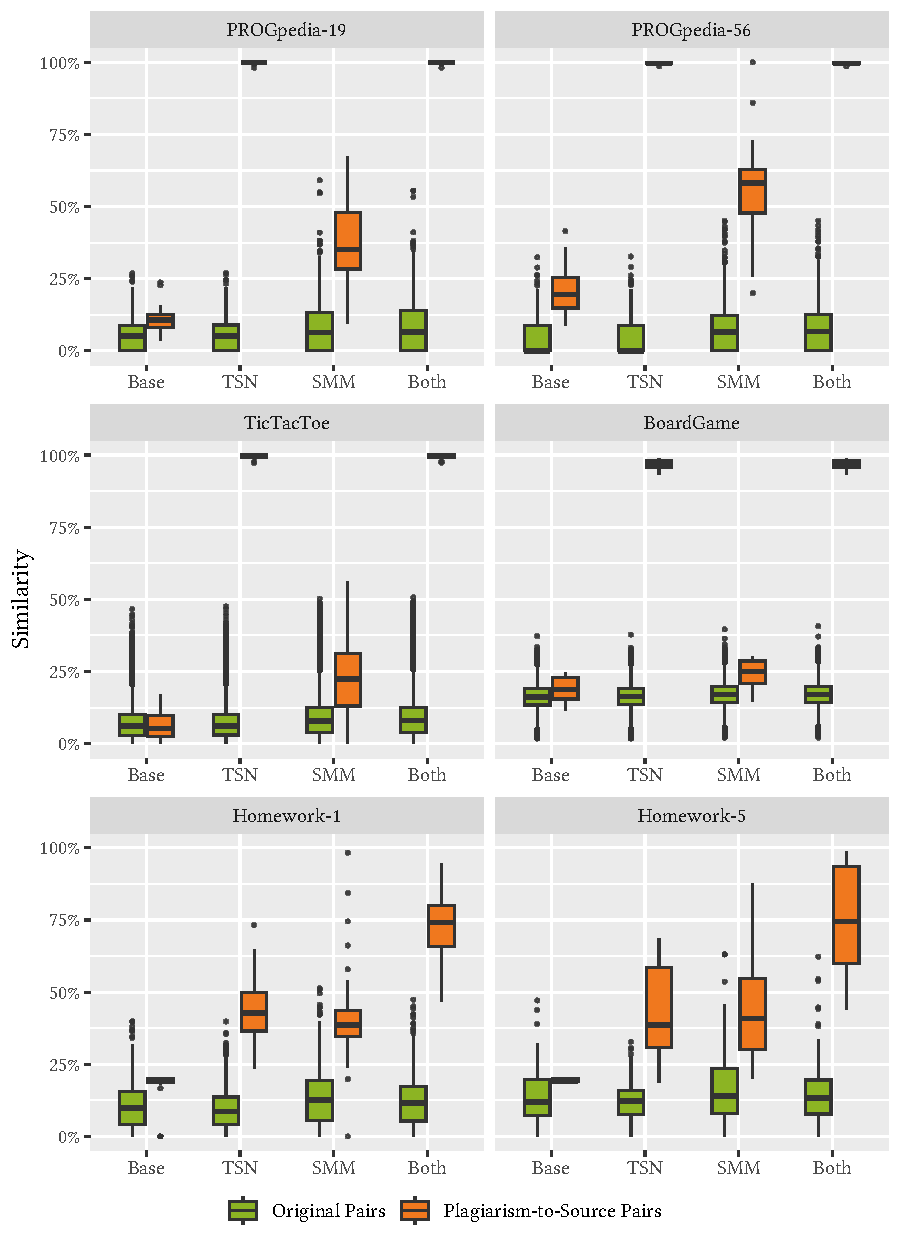
\includegraphics[width=\linewidth]{figures/disseval/eval-insertion_avg.similarity.pdf}
\caption[Evaluation Results: Insertion-based Obfuscation]{Similarity scores for original program pairs and \textbf{insertion-based plagiarism} pairs. Ideally, plagiarism pairs exhibit high similarity, while original pairs should exhibit low similarity.}
\label{fig:stage1-results}
\end{figure}

\subsubsection{Combination of Both}
We see strongly improved results when using both defense mechanisms together compared to the baseline.
With this defense mechanism, we even observe that JPlag is effectively immune to insertion-based attacks.
For the Java dataset, these results mirror the ones for subsequence match merging alone.
For the C++ datasets, however, the combination of both defense mechanisms shows an improvement over each individual.

For all six datasets, \autoref{fig:stage1-results} shows a significant similarity increase for plagiarism pairs (true positives).
Depending on the dataset, the median similarity values rise to between 74.10 percent (Homework-1) and 100.00 percent (PROGpedia-19).
We no longer observe any significant overlap between the plagiarism and original pairs, resulting in a clear separation between both types of pairs.

The median similarity \textit{differences} between plagiarism and original pairs (see \autoref{tab:diff-insert}) now range from 61.22 percentage points (Homework-5) to 93.42  percentage points (PROGpedia-19).
These results show that the combination of both defense mechanisms provides a substantial improvement over the baseline. 

As for both defense mechanisms individually, the improvement when using both is statistically and practically significant (see \autoref{tab:to-base-insert}).
The low p-values indicate statistical significance for the similarity increase for the plagiarism pairs.
Regarding practical significance, the effect size is very large for all of the six datasets.
Our results, thus, show that combining both defense mechanisms provides significant resilience against insertion-based obfuscation attacks for all six datasets.

\summaryBox{1.2}{Our defense mechanisms significantly increase the resilience against semantic preserving insertion-based obfuscation attacks. The median similarity differences increase, depending on the dataset, up to 99.65 percentage points, thus producing a complete separation of plagiarized and original programs. Thus, the degree of resilience effectively reflects near-immunity to insertion-based attacks. As discussed in \autoref{sec:eval-unrel}, the impact on the false positive rate is practically insignificant.}

\subsection{Alteration-based Obfuscation}\label{sec:eval-alter}
% FIGURE TEXT
\autoref{fig:stage2-results} shows the results for obfuscation attacks based on random alterations of the token sequence.
\autoref{tab:diff-alter} shows the corresponding statistical measures.
% ATTACK TYPE REFRESHER TEXT
As discussed, these attacks are simulated, meaning 25\% of the token sequence is directly replaced by another random token. While this is thus not a real obfuscation attack, it simulates the effect of a very strong obfuscation attacks. As these simulated alterations could be caused by both semantic-preserving and semantic-altering obfuscation attacks, we consider this evaluation state semantic-agnostic. However, as this simulated obfuscation is done after the tokenization, it cannot be evaluated with the Token Sequence normalization, which partially takes place \textit{during} the tokenization.
Thus, we only evaluate this obfuscation attack for subsequence match merging and the baseline.

\begin{table}[h]
	\centering
	\small
	\begin{tabular}{lrrrrrrrr}
		\toprule
		Dataset                       & Variant & Median    & Mean      & $Q_1$     & $Q_3$     & $\Delta$ Mean & $\Delta$ Median & $\Delta$ IQR \\ 
		\midrule
		\multirow{2}{*}{PROGpedia-19} & Base     & 23.82     & 25.34     & 18.24     & 32.83     & 19.61         & 18.76           & 9.34         \\ 
		                              & SMM      & \B{59.50} & \B{64.33} & \B{55.05} & \B{76.32} & \B{55.17}     & \B{53.15}       & \B{41.85}    \\ 
		\hline
		\multirow{2}{*}{PROGpedia-56} & Base     & 19.92     & 23.16     & 13.90     & 34.22     & 18.27         & 19.92           & 5.13         \\ 
		                              & SMM      & \B{68.59} & \B{66.31} & \B{47.00} & \B{88.70} & \B{58.05}     & \B{62.00}       & \B{34.81}    \\ 
		\hline
		\multirow{2}{*}{TicTacToe}    & Base     & 22.36     & 23.32     & 19.07     & 26.08     & 16.47         & 16.29           & 9.10         \\ 
		                              & SMM      & \B{48.97} & \B{49.48} & \B{42.10} & \B{57.89} & \B{40.65}     & \B{41.13}       & \B{29.58}    \\ 
		\hline
		\multirow{2}{*}{BoardGame}    & Base     & 23.05     & 23.06     & 21.87     & 25.03     & 6.88          & 6.86            & 2.90         \\ 
		                              & SMM      & \B{35.01} & \B{35.06} & \B{33.61} & \B{36.75} & \B{18.11}     & \B{18.05}       & \B{13.87}    \\ 
		\hline
        \multirow{2}{*}{Homework-1}   & Base     & 13.52     & 13.03     & 10.00     & 16.52     & 2.64          & 3.65            & -5.60        \\ 
		                              & SMM      & \B{40.39} & \B{42.23} & \B{33.05} & \B{50.73} & \B{29.19}     & \B{27.81}       & \B{13.55}    \\ 
		\hline
		\multirow{2}{*}{Homework-5}   & Base     & 10.77     & 12.69     & 6.28      & 20.86     & -0.70         & -1.23           & -13.40       \\ 
		                              & SMM      & \B{45.88} & \B{46.32} & \B{37.05} & \B{57.02} & \B{29.95}     & \B{31.86}       & \B{13.37}    \\ 
		\bottomrule
	\end{tabular}
	\caption[Evaluation Results: Alteration-based Obfuscation]{Statistical measures for plagiarism pairs and their differences ($\Delta$) from original pairs for \textbf{alteration-based obfuscation} (corresponds to \autoref{fig:stage2-results}). Higher values indicate better performance. Note that measures are expressed as percentages and their differences as percentage points.}
	\label{tab:diff-alter}
\end{table}

\begin{figure}
\centering
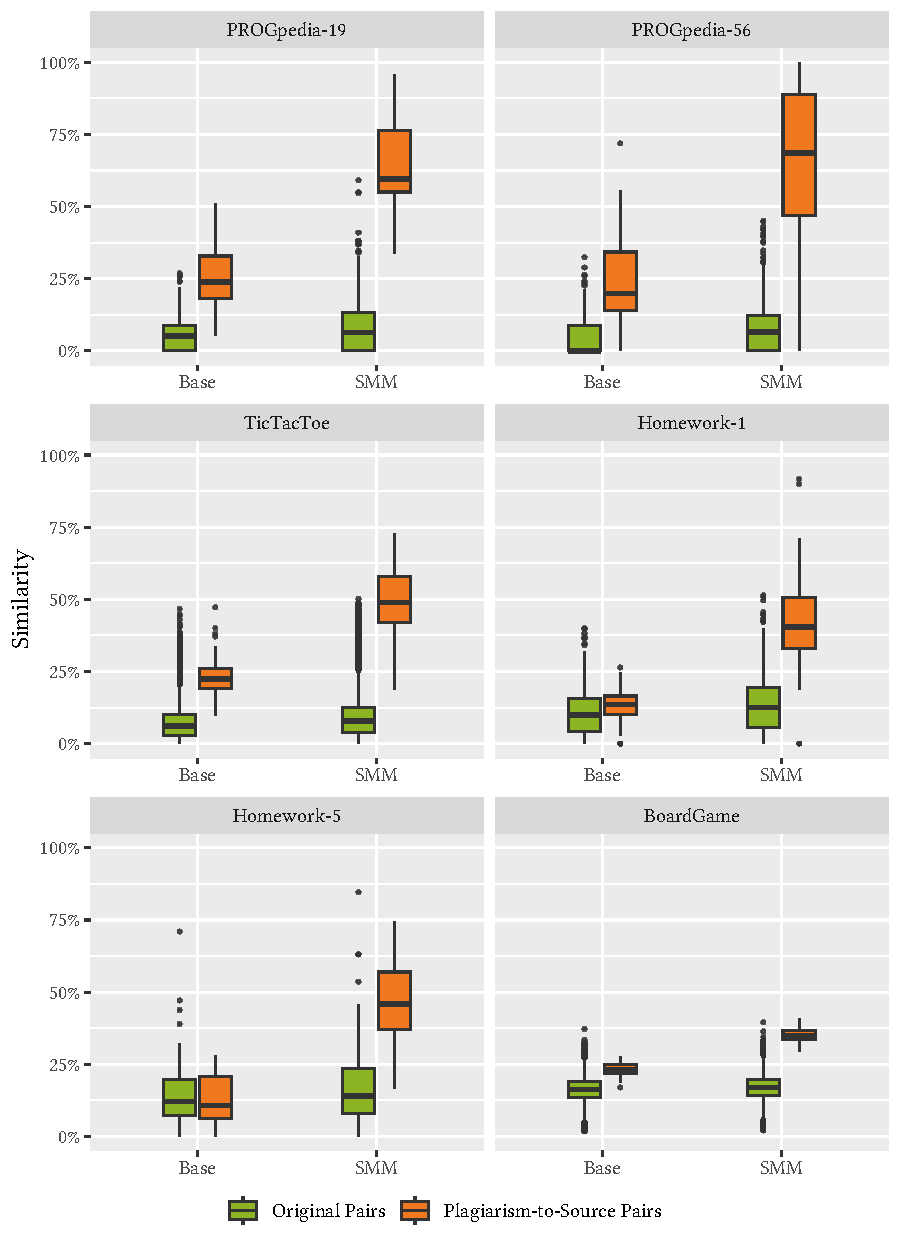
\includegraphics[width=\linewidth]{figures/disseval/eval-alteration_avg.similarity.pdf}
\caption[Evaluation Results: Alteration-based Obfuscation]{Similarity scores for original program pairs and \textbf{alteration-based plagiarism} pairs. Ideally, plagiarism pairs exhibit high similarity, while original pairs should exhibit low similarity.}
\label{fig:stage2-results}
\end{figure}

% ------------------------------------------------------- $
\begin{table}[h]
\centering
\small
%\setlength{\tabcolsep}{5pt}
\begin{tabular}{lrrrrrrrr}
  \toprule
Dataset & Variant & Pairs & $p$ & $W$ & $\delta$ & $\delta\,Int.$ & $\delta$ 95\% CI & n \\ 
  \midrule
   PROGpedia-19& SMM & P2S & 3e-06 & 378 & 0.962 & Very Large & [0.87, 0.99] & 27 \\ 
   PROGpedia-56& SMM & P2S & 3e-06 & 378 & 0.828 & Very Large & [0.59, 0.93] & 28 \\ 
   TicTacToe& SMM & P2S & 3.9e-10 & 1,275 & 0.934 & Very Large & [0.82, 0.98] & 50 \\ 
   BoardGame & SMM & P2S & 4.8e-05 & 210 & 1.000 & Very Large & [1.00, 1.00] & 20 \\ 
   Homework-1& SMM & P2S & < 1e-10 & 1,653 & 0.924 & Very Large & [0.77, 0.98] & 59 \\ 
   Homework-5& SMM & P2S & 0.00011 & 171 & 0.932 & Very Large & [0.75, 0.98] & 18 \\ 
   \bottomrule
\end{tabular}
\caption[Statistical Tests: Alteration-based Obfuscation]{One-sided Wilcoxon signed-rank test results for \textbf{alteration-based obfuscation} regarding the improvement by our defense mechanism compared to baseline (sig. level of $\alpha=0.01$, alternative hypothesis $H1=greater$, test statistic $W$, effect size via Cliff's delta $\delta$, its interpretation $\delta\,Int.$, its 95 percent confidence interval $CI$, and the sample size $n$). For plagiarism-to-source pairs (P2S), low $p$ and high $\delta$ are desirable.} 
\label{tab:to-base-alter}
\end{table}
 
% ------------------------------------------------------- $

\subsubsection{Baseline}
%
\autoref{fig:stage2-results} illustrates the significant impact of the simulated obfuscation attack on the baseline.
For the baseline, the median similarity values for plagiarism pairs (true positives) drop to between 10.77 percent (Homework-5) and 23.82 percent (PROGpedia-19), depending on the dataset.
This results in a clear overlap between plagiarism and original pairs across all datasets.
The overlap is particularly pronounced in the homework datasets, where the interquartile ranges of plagiarism and original pairs strongly intersect.

As shown in \autoref{tab:diff-alter}, the median similarity \textit{differences} between plagiarism and original pairs range from -0.70 percentage points (Homework-5) to 19.61 percentage points (PROGpedia-19). On the lower end, this indicates that the median similarity of plagiarism instances is actually \textit{lower} than that of unrelated programs. Even on the higher end, the difference of 19.61 percentage points offers limited separation between plagiarism pairs and unrelated originals. These baseline results demonstrate that the random alteration simulates the effects of a strong obfuscation attack.

\subsubsection{Subsequence Match Merging}
In contrast to the baseline, subsequence match merging produces strongly improved results.
For all six datasets, \autoref{fig:stage2-results} shows a significant similarity increase for plagiarism pairs (true positives).
The median similarity values rise, depending on the dataset, to between 35.01 percent (BoardGame) and 68.59 percent (PROGpedia-56).
Thus, the overlap is limited and mostly affects the lower quartile of the plagiarism pairs and the upper quartile of the original pairs.
This reduced overlap is also reflected when analyzing the similarity differences between plagiarism and original pairs (see \autoref{tab:diff-alter}).
The median similarity \textit{differences} between plagiarism and original pairs now range from 18.05 percentage points (BoardGame) to 62.00 percentage points (PROGpedia-56).
These results show that subsequence match merging provides a strong improvement over the baseline.

Furthermore, this improvement is clearly both statistically and practically significant, as shown by the results of the statistical test (see \autoref{tab:to-base-alter}).
Regarding statistical significance, the extremely low p-values indicate strong statistical significance for the similarity increase for the plagiarism pairs.
Regarding practical significance, the effect size is very high for all datasets, and thus, the increases are practically significant.
In sum, subsequence match merging provides significant resilience against alteration-based obfuscation attacks for all six datasets.
This means it facilitates detection despite randomly changing 25\% of the linearized program.

\summaryBox{1.3}{Subsequence Match Merging \textit{significantly} increases the resilience against semantic agnostic alteration-based obfuscation attacks. The median similarity differences increase, depending on the dataset, up to 42 percentage points, thus producing a clear separation between plagiarized and original programs. As discussed in \autoref{sec:eval-unrel}, the impact on the false positive rate is practically insignificant.}


\subsection{Refactoring-based Obfuscation}\label{sec:eval-refactor}
% FIGURE TEXT
\autoref{fig:stage2.5-results} shows the results for refactoring attacks based on a mix of different refactoring operations.
\autoref{tab:diff-refactor} shows the corresponding statistical measures.
% ATTACK TYPE REFRESHER TEXT
As discussed, the attack automatically applies semantic-preserving refactoring operations at random positions at the \ac{AST} level to obfuscate programs.
As the implementation of this obfuscation attack~\cite{Maisch2024} only supports Java programs, we evaluate this attack with four of the six datasets.

\begin{table}[h]
	\centering
	\small
	\begin{tabular}{lrrrrrrrr}
		\toprule
		Dataset      & Variant & Median    & Mean      & $Q_1$     & $Q_3$      & $\Delta$ Mean & $\Delta$ Median & $\Delta$ IQR \\ 			
		\midrule
		\multirow{4}{*}{PROGpedia-19} & Base & 18.82     & 23.21     & 14.74     & 29.64      & 17.48         & 13.76           & 5.83         \\ 
		 & TSN  & 18.82     & 22.48     & 14.43     & 27.53      & 16.73         & 13.70           & 5.49         \\ 
		 & SMM  & \B{42.29} & \B{38.63} & \B{27.35} & \B{49.59}  & \B{29.48}     & \B{35.93}       & \B{14.15}    \\ 
		 & Both & 36.26     & 37.15     & 26.23     & 48.21      & 27.93         & 29.69           & 12.35        \\ 
		\hline
		\multirow{4}{*}{PROGpedia-56} & Base & 18.20     & 21.55     & 6.42      & 30.97      & 16.66         & 18.20           & -2.34        \\ 
		 & TSN  & 15.47     & 20.85     & 6.43      & 31.10      & 16.34         & 15.47           & -2.22        \\ 
		 & SMM  & \B{42.62} & 37.02     & 21.33     & \B{50.94}  & 28.76         & \B{36.02}       & 9.13         \\ 
		 & Both & 41.32     & \B{37.21} & \B{24.05} & 50.40      & \B{29.09}     & 34.58           & \B{11.44}    \\ 
		\hline
		\multirow{4}{*}{TicTacToe}    & Base & 13.90     & 17.86     & 9.49      & 22.84      & 11.01         & 7.83            & -0.47        \\ 
		    & TSN  & 13.12     & 17.52     & 8.81      & 22.97      & 10.58         & 6.96            & -1.26        \\ 
		    & SMM  & \B{25.47} & \B{28.84} & \B{16.98} & \B{36.89 } & \B{20.02}     & \B{17.62}      & \B{4.48}     \\ 
		    & Both & 25.28     & 28.00     & 16.91     & 35.93      & 19.08         & 17.32           & 4.28         \\ 
		\hline
		\multirow{4}{*}{BoardGame}    & Base & 35.02     & 35.76     & 29.27     & 39.61      & 19.58         & 18.82           & 10.30        \\ 
		    & TSN  & 34.32     & 35.20     & 28.85     & 39.32      & 18.87         & 17.98           & 9.72         \\ 
		    & SMM  & \B{41.47} & \B{41.37} & \B{35.67} & \B{45.09 } & \B{24.42}     & \B{24.52}       & \B{15.92}    \\ 
		    & Both & 40.40     & 40.54     & 34.16     & 44.16      & 23.45         & 23.32           & 14.26        \\ 
		\bottomrule
	\end{tabular}
	\caption[Evaluation Results: Refactoring-based Obfuscation]{Statistical measures for plagiarism pairs and their differences ($\Delta$) from original pairs for \textbf{refactoring-based obfuscation} (corresponds to \autoref{fig:stage2.5-results}). Higher values indicate better performance. Note that measures are expressed as percentages and their differences as percentage points.}
	\label{tab:diff-refactor}
\end{table}

% ------------------------------------------------------- $
\begin{table}[h]
\centering
\small
\begin{tabular}{lrrrrrrrr}
  \toprule
Dataset & Variant & Pairs & $p$ & $W$ & $\delta$ & $\delta\,Int.$ & $\delta$ 95\% CI & n \\
        \midrule
   \multirow{3}{*}{{PROGpedia-19}}& TSN & P2S & 1 & 11 & -0.036 & Negligible & [-0.33, 0.26] & 27 \\ 
   & SMM & P2S & 6.5e-06 & 325 & 0.567 & Large & [0.28, 0.76] & 27 \\ 
   & Both & P2S & 5e-06 & 350 & 0.510 & Large & [0.21, 0.72] & 27 \\
     \hline
   \multirow{3}{*}{{PROGpedia-56}}& TSN & P2S & 0.31 & 108 & -0.015 & Negligible & [-0.31, 0.28] & 28 \\ 
   & SMM & P2S & 2.2e-05 & 253 & 0.462 & Medium & [0.16, 0.68] & 28 \\ 
   & Both & P2S & 6.5e-06 & 325 & 0.473 & Medium & [0.17, 0.69] & 28 \\ 
   \hline
   \multirow{3}{*}{{TicTacToe}} & TSN & P2S & 0.98 & 143 & -0.020 & Negligible & [-0.24, 0.21] & 50 \\ 
   & SMM & P2S & 5.7e-10 & 1,225 & 0.513 & Large & [0.30, 0.68] & 50 \\ 
   & Both & P2S & 5.7e-10 & 1,225 & 0.484 & Large & [0.27, 0.65] & 50 \\ 
  \hline 
   \multirow{3}{*}{{BoardGame}}& TSN & P2S & 1 & 14 & -0.065 & Negligible & [-0.40, 0.28] & 20 \\ 
   & SMM & P2S & 4.8e-05 & 210 & 0.430 & Medium & [0.06, 0.70] & 20 \\ 
   & Both & P2S & 4.8e-05 & 210 & 0.380 & Medium & [0.01, 0.66] & 20 \\
   \bottomrule
\end{tabular}
\caption[Statistical Tests: Refactoring-based Obfuscation]{One-sided Wilcoxon signed-rank test results for \textbf{refactoring-based obfuscation} regarding the improvement by our defense mechanism compared to baseline (sig. level of $\alpha=0.01$, alternative hypothesis $H1=greater$, test statistic $W$, effect size via Cliff's delta $\delta$, its interpretation $\delta\,Int.$, its 95 percent confidence interval $CI$, and the sample size $n$). For plagiarism-to-source pairs (P2S), low $p$ and high $\delta$ are desirable.} 
\label{tab:to-base-refactor}
\end{table} 
% ------------------------------------------------------- $

\subsubsection{Baseline}
\autoref{fig:stage2.5-results} illustrates the significant impact of refactoring-based obfuscation attack on the baseline.
For the baseline, the median similarity values for plagiarism pairs (true positives) drop to between 13.90 percent (TicTacToe) and 35.02 percent (BoardGame), depending on the dataset.
This results in a clear overlap between plagiarism and original pairs for all datasets except BoardGame. Here, the overlap is less pronounced and mostly affects the outliers of the original pairs. This is in line with the classification proposed in our threat model (see \autoref{fig:clone-types}), which illustrates that more complex obfuscation techniques are harder to apply broadly, which reduces the effectiveness for large programs such as the ones on the BoardGame datasets.

As shown in \autoref{tab:diff-refactor}, the median similarity \textit{differences} between plagiarism and original pairs range from 7.83 percentage points (TicTacToe) to 18.82 percentage points (BoardGame). This indicates a limited separation between plagiarism pairs and unrelated originals. Thus, refactoring is an effective obfuscation on the baseline JPlag.

\subsubsection{Token Sequence Normalization}
As the refactoring-based obfuscation does not rely on statement insertion or reordering, token sequence normalization has little to no effect. This, however, is expected, as it is not designed for refactoring-based obfuscation attacks.

For all six datasets, \autoref{fig:stage2.5-results} shows results that closely resemble the results for the baseline.
The median similarity values of the plagiarism pairs are even a bit lower compared to the baseline for three of four datasets. This reduction, however, is between 0.78 percentage points (TicTacToe) and 2.73 percentage points (PROGpedia-56)). Thus, the reduction is very subtle.
Consequently, this trend is also reflected when analyzing the similarity differences between plagiarism and original pairs (see \autoref{tab:diff-refactor}).
The median similarity \textit{differences} between plagiarism and original pairs range from 6.96 percentage points (TicTacToe) to 18.87 percentage points (BoardGame).

The results of the statistical test (see \autoref{tab:to-base-refactor}), however, show that this change is both statistically and practically insignificant.
Regarding statistical significance, the high p-values indicate no statistical significance similarity increase for the plagiarism pairs.
Regarding practical significance, the effect size even shows a reduction in similarity values through negative values for all three datasets. However, the effect size is close to zero, and the practical significance is thus negligible.
In sum, token sequence normalization provides, as expected, no significant resilience against refactoring-based obfuscation attacks, as the results are not significantly different compared to the baseline.


\subsubsection{Subsequence Match Merging}
In contrast to the baseline, subsequence match merging produces strongly improved results.
For all six datasets, \autoref{fig:stage3-results} shows a significant similarity increase for plagiarism pairs (true positives).
The median similarity values rise, depending on the dataset, to between 25.47 percent (TicTacToe) and 42.62 percent (PROGpedia-56).
Thus, the overlap is limited and mostly affects the lower quartile of the plagiarism pairs and the upper quartile of the original pairs.
This reduced overlap is also reflected when analyzing the similarity differences between plagiarism and original pairs (see \autoref{tab:diff-refactor}).
The median similarity \textit{differences} between plagiarism and original pairs now range from 17.62 percentage points (TicTacToe) to 36.02 percentage points (PROGpedia-56).
These results show that subsequence match merging provides a solid improvement over the baseline. 

Furthermore, this improvement is both statistically and practically significant, as shown by the results of the statistical test (see \autoref{tab:to-base-refactor}).
The low p-values indicate statistical significance for the similarity increase for the plagiarism pairs.
Regarding practical significance, the effect size is medium (BoardGame and PROGpedia-56) to large (TicTacToe, PROGpedia-19) for the datasets, and thus the increases are all practically significant.
In sum, subsequence match merging provides significant resilience against refactoring-based obfuscation attacks for all six datasets.
This means it facilitates detection despite the random application of many refactoring operations, which strongly change the structure of the programs.

\begin{figure}
\centering
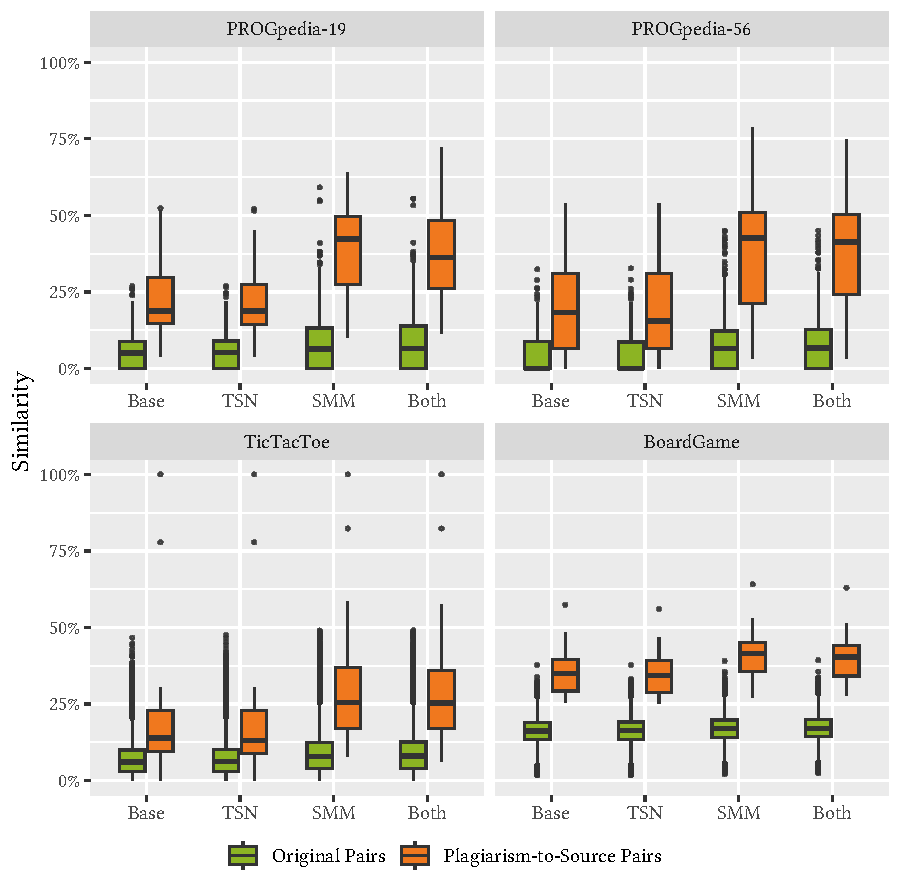
\includegraphics[width=\linewidth]{figures/disseval/eval-refactor_avg.similarity.pdf}
\caption[Evaluation Results: Refactoring-based Obfuscation]{Similarity scores for original program pairs and \textbf{refactoring-based plagiarism} pairs. Ideally, plagiarism pairs exhibit high similarity, while original pairs should exhibit low similarity.}
\label{fig:stage2.5-results}
\end{figure}


\subsubsection{Combination of Both}
When using both defense mechanisms together, we see strongly improved results compared to the baseline.
For all six datasets, \autoref{fig:stage3-results} shows a significant similarity increase for plagiarism pairs (true positives), mirroring the results for subsequence match merging on its own.
Depending on the dataset, the median similarity values rise to between 25.28 percent (TicTacToe) and 41.32 percent (PROGpedia-56).
As for subsequence match merging, the overlap is limited and mostly affects the lower quartile of the plagiarism pairs and the upper quartile of the original pairs.
%This is also reflected when analyzing the similarity differences between plagiarism and original pairs (see \autoref{tab:diff-refactor}).
The median similarity \textit{differences} between plagiarism and original pairs (see \autoref{tab:diff-refactor}) now range from 17.32 percentage points (TicTacToe) to 34.58  percentage points (PROGpedia-56).
Note that these results show a solid improvement over the baseline, which is minimally smaller than the one for subsequence match merging (one exception is PROGpedia-56; here, the combination of both has a slightly higher median difference). 

As for subsequence match merging, this improvement is statistically and practically significant (see \autoref{tab:to-base-refactor}).
The low p-values indicate statistical significance for the similarity increase for the plagiarism pairs.
Regarding practical significance, the effect size is medium (BoardGame and PROGpedia-56) to large (TicTacToe, PROGpedia-19) for the datasets.
In sum, the combination of both defense mechanisms provides significant resilience against refactoring-based obfuscation attacks for all six datasets.

\summaryBox{1.4}{Our defense mechanisms significantly increase the resilience against semantic preserving refactoring-based obfuscation attacks. The median similarity differences increase, depending on the dataset, up to 22 percentage points, thus strongly improving the separation between plagiarized and original programs. As discussed in \autoref{sec:eval-unrel}, the impact on the false positive rate is practically insignificant.}

\subsection{GPT-4-based Obfuscation}\label{sec:eval-gptobf}
% FIGURE TEXT
% ATTACK TYPE REFRESHER TEXT
\autoref{fig:stage3-results} shows the results for obfuscation attacks via GPT-4 prompts. 
\autoref{tab:diff-gpt-obf} shows the corresponding statistical measures.
We used 15 different prompts, asking the LLM to alter the program without changing its behavior. %However, we did not check if the behavior was actually preserved. \todoNils{Wurde das Verhalten manchmal verändert?}
There are no guarantees that the behavior will be preserved, thus making this obfuscation attack a semantic-agnostic one.

It is important to note that the BoardGame dataset was excluded from the evaluation involving AI-based datasets. This dataset originates from a final exam and is highly sensitive. Consequently, we must not submit the programs to the OpenAI server hosting GPT-4 as part of the obfuscation process.

\begin{table}[h]
	\centering
	\small
	\begin{tabular}{lrrrrrrrr}
		\toprule
		Dataset                       & Variant & Median    & Mean      & $Q_1$     & $Q_3$     & $\Delta$ Mean & $\Delta$ Median & $\Delta$ IQR \\ 
		\midrule
		\multirow{4}{*}{PROGpedia-19} & Base     & 54.59     & 54.12     & 28.06     & 81.04     & 48.39         & 49.53           & 19.15        \\ 
		                               & TSN      & 54.74     & 54.84     & 28.82     & 80.95     & 49.08         & 49.61           & 19.88        \\ 
		                               & SMM      & 73.95     & 63.46     & 36.51     & 92.34     & 54.31         & 67.59           & 23.31        \\ 
		                               & Both     & \B{74.79} & \B{63.60} & \B{38.32} & \B{92.98} & \B{54.38}    & \B{68.22}       & \B{24.44}    \\ 
		\hline
		\multirow{4}{*}{PROGpedia-56} & Base     & 66.67     & 61.76     & 46.67     & 77.96     & 56.87         & 66.67           & 37.91        \\ 
		                               & TSN      & 69.40     & 63.92     & 45.05     & 83.92     & 59.40         & 69.40           & 36.41        \\ 
		                               & SMM      & \B{84.43} & \B{75.37} & \B{65.76} & \B{92.60} & \B{67.11}    & \B{77.84}       & \B{53.56}    \\ 
		                               & Both     & 83.07     & 75.10     & 63.11     & 92.59     & 66.98         & 76.32           & 50.50        \\ 
		\hline
		\multirow{4}{*}{TicTacToe}    & Base     & 28.20     & 35.60     & 11.25     & 61.05     & 28.75         & 22.13           & 1.28         \\ 
		                               & TSN      & 27.98     & 37.50     & 12.32     & 62.26     & 30.56         & 21.83           & 2.25         \\ 
		                               & SMM      & \B{39.02} & 44.96     & 17.68     & 75.65     & 36.13         & \B{31.18}       & 5.16         \\ 
		                               & Both     & 38.07     & \B{45.53} & \B{20.11} & \B{75.70} & \B{36.61}     & 30.13           & \B{7.48}     \\ 
		\hline
		\multirow{4}{*}{Homework-1}   & Base     & 19.74     & 27.71     & 9.70      & 42.81     & 17.32         & 9.86            & -5.90        \\ 
		                               & TSN      & 15.47     & 26.44     & 7.88      & 42.50     & 17.07         & 6.83            & \B{-5.77}    \\ 
		                               & SMM      & \B{22.90} & \B{32.69} & \B{10.49} & 48.27     & \B{19.65}     & \B{10.32}       & -9.01        \\ 
		                               & Both     & 19.09     & 31.42     & 8.35      & \B{48.96} & 19.42         & 7.47            & -9.08        \\ 
		\hline
		\multirow{4}{*}{Homework-5}   & Base     & 41.33     & 50.37     & 27.02     & 77.79     & 36.97         & 29.34           & 7.34         \\ 
		                               & TSN      & 36.26     & 46.13     & 20.03     & 73.68     & 34.48         & 23.98           & 4.19         \\ 
		                               & SMM      & \B{50.68} & \B{57.54} & \B{32.45} & 89.24     & \B{41.62}     & \B{36.70}       & \B{8.79}     \\ 
		                               & Both     & 49.06     & 53.90     & 24.40     & \B{90.91} & 39.31         & 35.71           & 4.82         \\ 
		\bottomrule  
	\end{tabular}
	\caption[Evaluation Results: AI-based Obfuscation]{Statistical measures for plagiarism pairs and their differences ($\Delta$) from original pairs for \textbf{AI-based obfuscation} (corresponds to \autoref{fig:stage3-results}). Higher values indicate better performance. Note that measures are expressed as percentages and their differences as percentage points.}
	\label{tab:diff-gpt-obf}
\end{table}


% ------------------------------------------------------- $
\begin{table}[h]
\centering
\small
\begin{tabular}{lrrrrrrrr}
  \toprule
Dataset & Variant & Pairs & $p$ & $W$ & $\delta$ & $\delta\,Int.$ & $\delta$ 95\% CI & n \\ 
  \midrule 
   \multirow{3}{*}{{PROGpedia-19}} & TSN & P2S & 0.0027 & 893 & 0.019 & Negligible & [-0.17, 0.20] & 74 \\ 
   & SMM & P2S & < 1e-10 & 1,485 & 0.210 & Small & [0.02, 0.38] & 74 \\ 
   & Both & P2S & < 1e-10 & 2,216 & 0.209 & Small & [0.02, 0.38] & 74 \\ 
      \hline 
   \multirow{3}{*}{{PROGpedia-56}} & TSN & P2S & 0.025 & 971 & 0.077 & Negligible & [-0.11, 0.26] & 75 \\ 
   & SMM & P2S & < 1e-10 & 1,540 & 0.371 & Medium & [0.19, 0.53] & 75 \\ 
   & Both & P2S & < 1e-10 & 2,136 & 0.360 & Medium & [0.18, 0.52] & 75 \\ 
      \hline
   \multirow{3}{*}{{TicTacToe}} & TSN & P2S & 5.2e-08 & 1,107 & 0.042 & Negligible & [-0.14, 0.22] & 75 \\ 
   & SMM & P2S & < 1e-10 & 1,770 & 0.194 & Small & [0.01, 0.37] & 75 \\ 
   & Both & P2S & < 1e-10 & 2,342 & 0.210 & Small & [0.03, 0.38] & 75 \\ 
      \hline
   \multirow{3}{*}{{Homework-1}} & TSN & P2S & 0.89 & 913 & -0.046 & Negligible & [-0.23, 0.14] & 74 \\ 
   & SMM & P2S & 2e-06 & 406 & 0.075 & Negligible & [-0.11, 0.26] & 74 \\ 
   & Both & P2S & 0.003 & 1,536 & 0.024 & Negligible & [-0.16, 0.21] & 74 \\ 
      \hline
   \multirow{3}{*}{{Homework-5}}& TSN & P2S & 1 & 229 & -0.115 & Negligible & [-0.29, 0.07] & 75 \\ 
   & SMM & P2S & 2.7e-09 & 1,035 & 0.153 & Small & [-0.03, 0.33] & 75 \\ 
   & Both & P2S & 0.11 & 1,260 & 0.047 & Negligible & [-0.14, 0.23] & 75 \\ 
   \bottomrule
\end{tabular}
\caption[Statistical Tests: AI-based Obfuscation]{One-sided Wilcoxon signed-rank test results for \textbf{AI-based obfuscation} regarding the improvement by of our defense mechanism compared to baseline (sig. level of $\alpha=0.01$, alternative hypothesis $H1=greater$, test statistic $W$, effect size via Cliff's delta $\delta$, its interpretation $\delta\,Int.$, its 95 percent confidence interval $CI$, and the sample size $n$). For plagiarism-to-source pairs (P2S), low $p$ and high $\delta$ are desirable.} 
\label{tab:to-base-gpt-obf}
\end{table}
 
% ------------------------------------------------------- $

\subsubsection{Baseline}
\autoref{fig:stage3-results} illustrates the impact of GPT-4-based obfuscation via 15 different prompts.
For JPlag as a baseline, we observe that GPT-based obfuscation attacks can be very effective.
The median similarity values for plagiarism pairs (true positives) drop to between 19.74 percent (Homework-5) and 66.67 percent (PROGpedia-56), depending on the dataset.
Note that this range is higher than usual.

For the different datasets, we observe varying overlaps between plagiarism and original pairs. The strongest overlap is observed for Homework-1, where even the interquartile ranges overlap. The overlap is less pronounced for the PROGpedia datasets.
As shown in \autoref{tab:diff-gpt-obf}, the median similarity \textit{differences} between plagiarism and original pairs range from 9.86 percentage points (Homework-1) to 66.67 percentage points (PROGpedia-56). 
This indicates a limited separation between plagiarism pairs and unrelated originals, especially for the TicTacToe and Homework datasets. 

Note that the variance in the effectiveness of the attack due to the prompt choice is on the same magnitude as the variance between datasets (see \autoref{fig:stage3-results-byprompt}). 
While there are \textit{some} prompts (like prompts 7 and 8) that vary strongly in their effectiveness, most prompts are similar. Interestingly, the dataset itself has arguably a bigger impact on the obfuscation effectiveness than the prompt choice.

It is not surprising that different prompts vary in effectiveness. It is surprising, however, that the effectiveness strongly depends on the dataset. Furthermore, it does not correlate to the language of the datasets, the average size of the programs, or the number of programs in the datasets.
Rather, it seems that it mainly depends on the assignment and the domain to be modeled to solve it.
Consequently, AI-based obfuscation is an effective obfuscation attack. However, it is \textit{less reliable} than algorithmic obfuscation attacks due to the observed high variance.

\begin{figure}
\centering
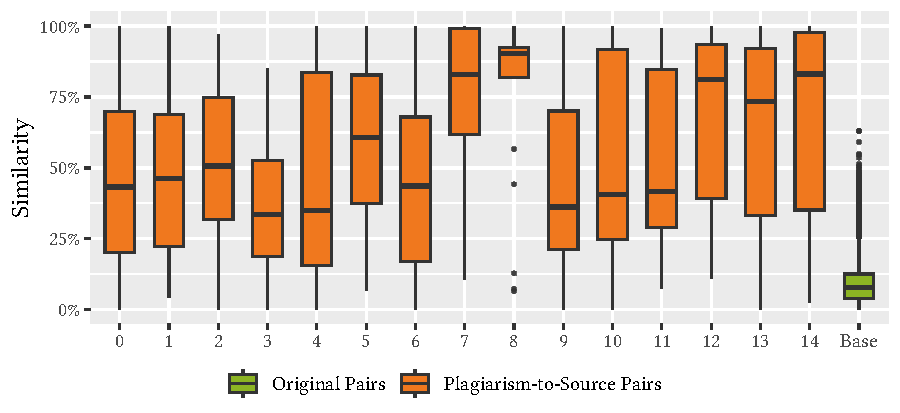
\includegraphics[width=\linewidth]{figures/disseval/eval-chatgpt-obf_avg.similarity-byprompt.pdf}
\caption[Evaluation Results: AI-based Obfuscation by Prompt]{Similarity scores for original program pairs (denoted as \textit{Base}) and \textbf{AI-based plagiarism} pairs by prompt (obfuscation with 15 varying GPT-4 prompts denoted by numbers from 0 to 14). Note that for this illustration, the results of all datasets are merged. Ideally, plagiarism pairs exhibit high similarity, while original pairs should exhibit low similarity.}
\label{fig:stage3-results-byprompt}
\end{figure}


\subsubsection{Token Sequence Normalization}

As GPT-4-based obfuscation relies on various modifications, it is reasonable to expect only a limited effect via token sequence normalization, which targets statement insertion and statement reordering. For all five datasets, \autoref{fig:stage3-results} shows results similar to the baseline.

Depending on the datasets, the median similarity values of the plagiarism pairs (true positives) are either slightly lower or slightly higher compared to the baseline. This difference, however, is minimal, ranging from -5.07 (Homework-5) to 2.37 percentage points (PROGpedia-56). 

We observe a similar effect when looking at the similarity differences between plagiarism and original pairs (see \autoref{tab:diff-gpt-obf}).
The median similarity \textit{differences} between plagiarism and original pairs range from 6.83 percentage points (Homework-1) to 69.40 percentage points (PROGpedia-56).
These values are similar to the baseline. While slightly better for both PROGpedia datasets, they are worse for both Homework datasets, which consist of C++ programs. This could indicate that GPT-4 uses different changes for C++ than for Java code.

The results of the statistical test (see \autoref{tab:to-base-gpt-obf}) show \textit{some} statistical significance; however, they show no practical significance.
Regarding statistical significance, we observe low p-values for the improvements with the PROGpedia-19 and the TicTacToe datasets, thus indicating statistical significance.
For the other three datasets, however, the p-values above the selected $\alpha$, thus representing statistically insignificant results.
Regarding practical significance, the effect size shows reduced similarity values through negative values for the Homework datasets. However, the effect size is close to zero for all datasets, and the practical significance is thus negligible.
In sum, token sequence normalization provides no significant resilience against GPT-4-based obfuscation attacks. However, it also does not bring any significant drawbacks.


\subsubsection{Subsequence Match Merging}
In contrast to the baseline, subsequence match merging produces strongly improved results.
For all six datasets, \autoref{fig:stage3-results} shows a significant similarity increase for plagiarism pairs (true positives).
Depending on the dataset, the median similarity values rise to between 22.90 percent (Homework-1) and 84.43 percent (PROGpedia-56).
Thus, the overlap is limited and mostly affects the lower quartile of the plagiarism pairs and the upper quartile of the original pairs.
This reduced overlap is also reflected when analyzing the similarity differences between plagiarism and original pairs (see \autoref{tab:diff-gpt-obf}).
The median similarity \textit{differences} between plagiarism and original pairs now range from 10.32 percentage points (Homework-1) to 77.84 percentage points (PROGpedia-56).
These results show that subsequence match merging provides a solid improvement over the baseline. 

Furthermore, this improvement is statistically significant for all datasets and practically significant for all but one, as shown by the results of the statistical test (see \autoref{tab:to-base-gpt-obf}).
Regarding statistical significance, the low p-values indicate strong statistical significance for the similarity increase for the plagiarism pairs.
Regarding practical significance, the effect size varies depending on the dataset. For Homework-1, the effect size is relatively small; thus, the practical significance is negligible (although statistical significance is given).
The effect size for the other five datasets, however, is medium to small, indicating practical significance.
Note that the high variance in plagiarism pair similarities affects the effect size measure~\cite{Grissom2012}. If the data has high variance, it is possible that even with large differences, the overall effect size appears small due to overlapping data points. Due to the use of 15 different prompts, the plagiarism pairs have a high variance in similarity values.

Thus, the increases are practically significant for all but one dataset.
In sum, subsequence match merging provides significant resilience against AI-based obfuscation. As previously stated, the strength of the obfuscation varies strongly on the dataset. Furthermore, the obfuscation attack is semantic agnostic, thus proving a further challenge.
Nevertheless, subsequence match merging improves detection despite AI-based obfuscation leveraging various changes, on which the defense mechanism can make very few assumptions.

\subsubsection{Combination of Both}
When using both defense mechanisms together, we observe strongly improved results compared to the baseline.
For all six datasets, \autoref{fig:stage3-results} shows a significant similarity increase for plagiarism pairs (true positives), mirroring the results for subsequence match merging on its own.
Depending on the dataset, the median similarity values rise to between 19.09 percent (Homework-1) and 83.07 percent (PROGpedia-56).
As for subsequence match merging, the overlap is limited and mostly affects the lower quartile of the plagiarism pairs and the upper quartile of the original pairs.
%This reduced overlap is also reflected when analyzing the similarity differences between plagiarism and original pairs (see \autoref{tab:diff-gpt-obf}).
The median similarity \textit{differences} between plagiarism and original pairs (see \autoref{tab:diff-gpt-obf} now range from 7.47 percentage points (Homework-1) to 76.32 percentage points (PROGpedia-56).
These results show a solid improvement over the baseline, which is minimally smaller than the one for subsequence match merging (one exception is PROGpedia-19; here, it is the other way around). 

This improvement is statistically significant for all datasets but one and practically significant for all but two, as shown by the results of the statistical test (see \autoref{tab:to-base-gpt-obf}).
Regarding statistical significance, the low p-values indicate strong statistical significance for the similarity increase for the plagiarism pairs, with the exception of Homework-5, where the p-value is 0.11.
Regarding practical significance, the effect size varies depending on the dataset. For both homework datasets, the effect size is relatively small; thus, the practical significance is negligible.
It is noteworthy that the homework datasets consist of small C++ programs, where AI-based obfuscation seems more effective. Note that this obfuscation is semantic-agnostic; thus, the behavior of the 75 programs each could deviate from the original.
Nevertheless, the effect size for the other four datasets is medium to small, indicating practical significance. As previously noted, the high variance in plagiarism pair similarities affects the effect size measure, leading to smaller effect size values.

In sum, combining both defense mechanisms provides significant resilience against AI-based obfuscation for the four Java datasets. However, the significance is limited for the two C++ datasets.
Yet, our defense mechanisms improve detection despite the potentially disruptive nature of AI-based obfuscation.

\summaryBox{1.5}{Our defense mechanisms significantly increase the resilience against semantic agnostic AI-based obfuscation attacks. The median similarity differences increase, depending on the dataset, up to 19 percentage points, thus improving the separation between plagiarized and original programs, albeit to a lesser degree than other attack types. As discussed in \autoref{sec:eval-unrel}, the impact on the false positive rate is practically insignificant.}

\begin{figure}
\centering
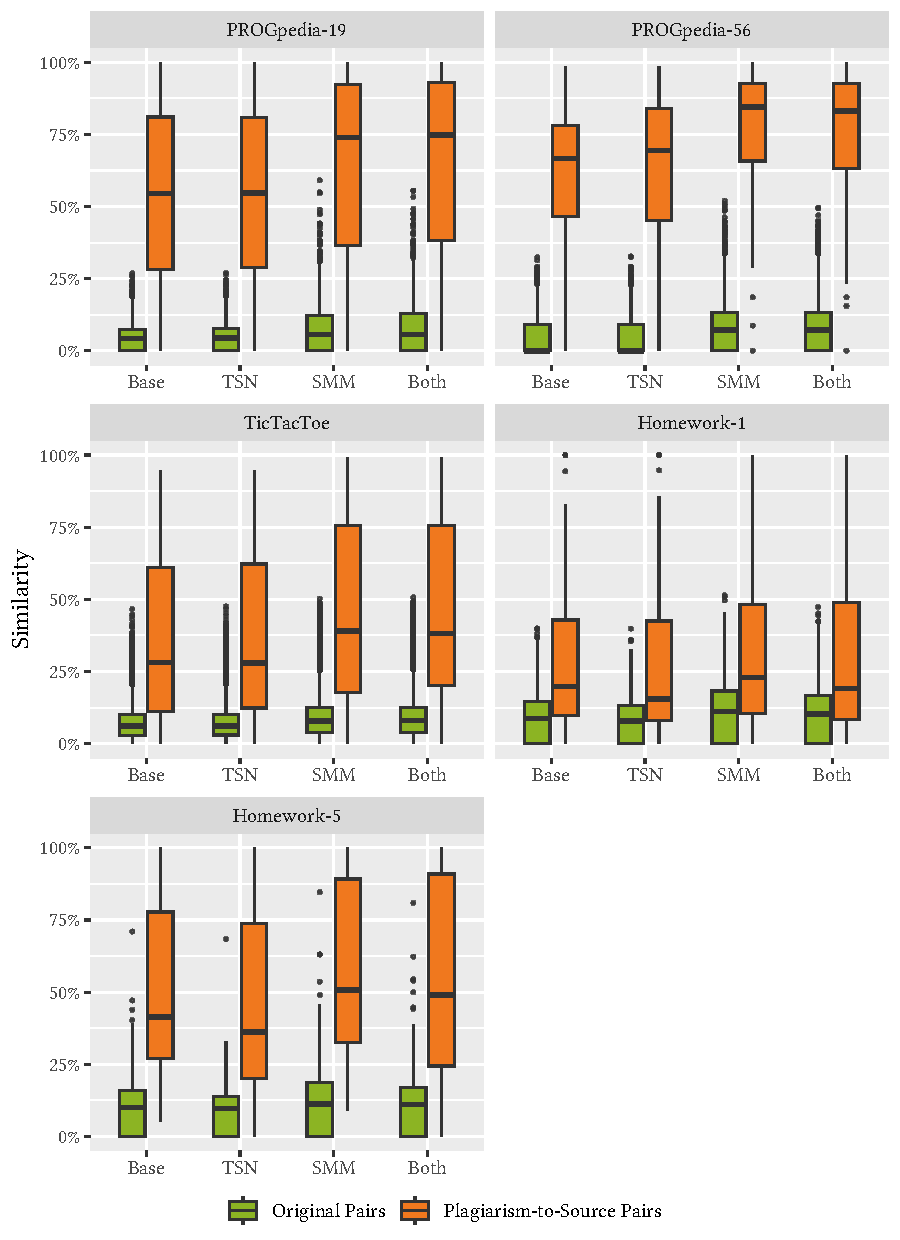
\includegraphics[width=\linewidth]{figures/disseval/eval-chatgpt-obf_avg.similarity.pdf}
\caption[Evaluation Results: AI-based Obfuscation]{Similarity scores for original program pairs and \textbf{AI-based plagiarism} pairs (obfuscation with 15 varying GPT-4 prompts). Ideally, plagiarism pairs exhibit high similarity, while original pairs should exhibit low similarity. }
\label{fig:stage3-results}
\end{figure}

\subsection{GPT-4-generated Programs}\label{sec:eval-gptgen}

% FIGURE TEXT
% ATTACK TYPE REFRESHER TEXT
\autoref{fig:stage3-results} shows the results for obfuscation attacks via GPT-4 prompts. 
\autoref{tab:diff-gpt-obf} shows the corresponding statistical measures.
We used 15 different prompts, asking the LLM to alter the program without changing its behavior. %However, we did not check if the behavior was actually preserved. \todoNils{Wurde das Verhalten manchmal verändert?}
There are no guarantees that the behavior will be preserved, thus making this obfuscation attack a semantic-agnostic one.

It is important to note that the BoardGame dataset was excluded from the evaluation involving AI-based datasets. This dataset originates from a final exam and is highly sensitive. Consequently, we must not submit the programs to the OpenAI server hosting GPT-4 as part of the obfuscation process.




\autoref{fig:stage4-results} shows the results for programs generated via GPT-4 based on the assignment description.
\autoref{tab:diff-gpt-gen} shows the corresponding statistical measures.
Unlike in the previous three evaluation stages, we \textit{technically} do not employ obfuscation attacks. The generated programs are not derived from human-made programs. 
Thus, our comparison focuses solely on how the similarity among generated programs differs from that of unrelated human programs.

Although our defense mechanisms are not specifically designed for this scenario, it is worth exploring whether they enhance the detection of AI-generated programs.
If these mechanisms enable us to differentiate between pairs of AI-generated programs and unrelated ones, we can detect AI-generated submissions in practice as long as more than one student chooses to use the same language model.

Since this evaluation stage required the full textual assignment description, we could only perform it on the TicTacToe dataset. As with the previous evaluation stage, the BoardGame dataset and the underlying task were excluded due to their sensitive nature.

\begin{table}[h]
	\centering
	\begin{tabular}{lrrrrrrrrr}
		\toprule
		Dataset                    & Variant & Median    & Mean      & $Q_1$     & $Q_3$     & $\Delta$ Mean & $\Delta$ Median & $\Delta$ IQR \\ 
		\midrule
	    \multirow{4}{*}{TicTacToe} & Base     & 20.63     & 22.53     & 12.53     & 31.51     & 15.67         & 14.57           & 2.57         \\ 
		                           & TSN      & 19.62     & 20.72     & 12.47     & 28.25     & 13.78         & 13.46           & 2.40         \\ 
		                           & SMM      & \B{28.94} & \B{29.60} & \B{18.27} & \B{39.72} & \B{20.77}     & \B{21.10}       & \B{5.75}    \\ 
		                           & Both     & 28.18     & 28.98     & 18.18     & 38.65     & 20.06         & 20.24           & 5.55         \\ 
		\bottomrule
	\end{tabular}
	\caption[Evaluation Results: AI-based Generation]{Statistical measures for plagiarism pairs and their differences ($\Delta$) from original pairs for \textbf{AI-based generation} (corresponds to \autoref{fig:stage4-results}). Higher values indicate better performance. Note that measures are expressed as percentages and their differences as percentage points.}
	\label{tab:diff-gpt-gen}
\end{table}

% ------------------------------------------------------- $
\begin{table}[h]
\centering
\small
%\setlength{\tabcolsep}{5pt}
\begin{tabular}{lrrrrrrrr}
  \toprule
Dataset & Variant & Pairs & $p$ & $W$ & $\delta$ & $\delta\,Int.$ & $\delta$ 95\% CI & n \\ 
  \midrule
   \multirow{3}{*}{{TicTacToe}} & TSN & FG & 1 & 120,687 & -0.072 & Negligible & [-0.12, -0.03] & 1,225 \\ 
    & SMM & FG & < 1e-10 & 334,971 & 0.271 & Small & [0.23, 0.31] & 1,225 \\ 
    & Both & FG & < 1e-10 & 416,672 & 0.256 & Small & [0.21, 0.30] & 1,225 \\ 
   \bottomrule
\end{tabular}
\caption[Statistical Tests: AI-based Generation]{One-sided Wilcoxon signed-rank test results for \textbf{AI-based generation} regarding the improvement by our defense mechanism compared to baseline (sig. level of $\alpha=0.05$, alternative hypothesis $H1=greater$, test statistic $W$, effect size via Cliff's delta $\delta$, its interpretation $\delta\,Int.$, its 95 percent confidence interval $CI$, and the sample size $n$). For Fully-Generated Pairs (FG), low $p$ and high $\delta$ are desirable.} 
\label{tab:to-base-gpt-gen}
\end{table}
 
% ------------------------------------------------------- $

\subsubsection{Baseline}
\autoref{fig:stage4-results} illustrates the results for GPT-4-generated programs.
For the baseline, the similarity values for generated program pairs (true positives) are mostly below 50 percent, with a median similarity of 20.63 percent.
This reflects the inherent indeterminism in generative AI, as these programs were generated from the same assignment description.
However, the similarity of unrelated human-made programs for the same assignment is mostly below 25 percent, with a median similarity of 6,06 percent.
This means that even for our baseline, the generated programs are significantly more similar to each other than human-made programs.

Nevertheless, there is still some overlap. 
As shown in \autoref{tab:diff-gpt-gen}, the median similarity \textit{difference} between AI-generated and original pairs is 14.57 percentage points. 
This indicates a limited separation between human-made and AI-generated programs. Furthermore, this median similarity difference is at a similar level as for refactoring- and alteration-based obfuscation attacks.
However, it is significantly higher than for insertion-based obfuscation attacks, where the median difference was slightly \textit{below} zero (-0.78 percentage points).
In summary, despite the increased similarity of AI-generated programs compared to human-made programs for our baseline, it may still be possible to evade detection, thus motivating the need for mechanisms to improve that.

\subsubsection{Token Sequence Normalization}
As token sequence normalization is designed to deal with statement insertion and statement reordering, we do not expect much impact on AI-generated programs.
AI-generated programs will contain little to no dead code, and the impact of statement order is not big enough on its own.

\autoref{fig:stage4-results} shows, as expected, little to no difference compared to the baseline.
The median similarity of the plagiarism pairs is 19.62 percent, which is slightly lower than the baseline (20.63 percent).
When looking at the similarity \textit{differences} between plagiarism and original pairs (see \autoref{tab:diff-gpt-gen}), we also see a slight reduction, as the difference is 13.46 (instead of 14.57) percentage points when using token sequence normalization.

The results of the statistical test (see \autoref{tab:to-base-gpt-gen}) show that this change is both statistically and practically insignificant.
With a p-value of 1, the improvement when using token sequence normalization over the baseline is not statistically significant.
While the effect size shows a slight reduction in similarity values (thus reflecting the decreased median similarity difference), it is close to zero, and the practical significance is thus negligible.
In sum, token sequence normalization provides, as expected, no significant improvement in resilience against AI-generated programs but also does not have significant drawbacks.

\subsubsection{Subsequence Match Merging}
In contrast to the baseline, subsequence match merging produces strongly improved results.
\autoref{fig:stage4-results} shows a significant similarity increase for plagiarism pairs (true positives).
Compared to the baseline, the median similarity value rises by 8.31 percentage points to 28.94 percent.
Thus, the overlap is decreased and mostly affects the upper quartile of the original pairs.

This reduced overlap is also reflected when analyzing the similarity differences between plagiarism and original pairs (see \autoref{tab:diff-gpt-gen}).
The median similarity \textit{difference} between plagiarism and original pairs is increased to 21.10 percentage points.
These results show that subsequence match merging provides a solid improvement over the baseline.

Furthermore, this improvement is both statistically and practically significant, as shown by the results of the statistical test (see \autoref{tab:to-base-gpt-gen}).
The low p-values indicate strong statistical significance for the similarity increase of the plagiarism pairs.
Regarding practical significance, the effect size is small but still relevant in practice.
In sum, subsequence match merging provides significant improvement for the detection of AI-generated programs.
These results are remarkable, given that the defense mechanism is not designed to detect AI-generated programs. The fact that it improves detection for them is surprising but highlights its versatility.
%This means the defense mechanism facilitates detection despite not being designed to detect AI-generated programs at all.

\subsubsection{Combination of Both}
When using both defense mechanisms together, we observe strongly improved results compared to the baseline.
\autoref{fig:stage4-results} shows a significant similarity increase for plagiarism pairs (true positives), mirroring the results for subsequence match merging.
Compared to the baseline, the median similarity value rises by 7.55 percentage points to 28.18 percent.
As for subsequence match merging, the overlap is decreased and mostly affects the upper quartile of the original pairs.

The median similarity \textit{difference} (see \autoref{tab:diff-gpt-gen}) between plagiarism and original pairs is increased to 20.24 percentage points.
These results show a solid improvement over the baseline, which is insignificantly smaller than the one for subsequence match merging. 

As for subsequence match merging, this improvement is both statistically and practically significant, as shown by the results of the statistical test (see \autoref{tab:to-base-gpt-gen}).
The low p-values indicate strong statistical significance for the similarity increase of the plagiarism pairs, while the effect size suggests practical significance.
In sum, combining both defense mechanisms provides significant improvement in the detection of AI-generated programs.
This improvement is nearly identical to the one for subsequence match merging, so combining both defense mechanisms has no drawbacks.

\summaryBox{1.6}{Our defense mechanisms, while not designed for this purpose, significantly increase the detection rate of AI-generated programs. The median similarity difference to human programs increases by 6.5 percentage points, thus improving the separation between plagiarized and original programs moderately but yet significantly. As discussed in \autoref{sec:eval-unrel}, the impact on the false positive rate is practically insignificant.}


\begin{figure}
\centering
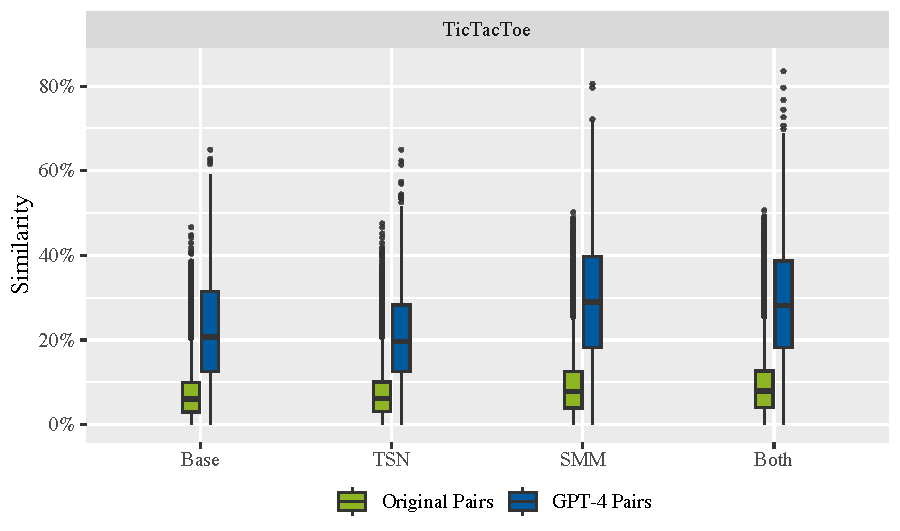
\includegraphics[width=\linewidth]{figures/disseval/eval-chatgpt-full_avg.similarity.pdf}
\caption[Evaluation Results: AI-based Generation]{Similarity scores for original (human) program pairs and pairs of \textbf{AI-generated programs} (based on GPT-4 and the assignment description). Ideally, generated pairs exhibit high similarity, while original pairs should exhibit low similarity.}
\label{fig:stage4-results}
\end{figure}

\subsection{Threshold-based Plagiarism}\label{sec:eval-mossad}

In the previous sections, we evaluated each variant (Base, TSN, SMM, and Both) attack using identical plagiarism instances for a given obfuscation attack.
This allowed us to directly compare the effectiveness of the variants.
Threshold-based obfuscation attacks, like \mossad, rely on a plagiarism detector to verify whether the obfuscated instance is sufficiently dissimilar from its source.
In \autoref{sec:eval-insert}, we configured \mossad to use the baseline (JPlag without defense mechanisms) for this purpose.
This raises the question of how our defense mechanisms affect threshold-based attacks when enabled during the obfuscation process.

To answer this, we chose ten random programs for each of the Homework datasets (\mossad is only compatible with C++ programs) and executed \mossad for each one.
Note that the average size of these programs is small. The Homework-1 dataset has an average size of 105 LoC per program, and the Homework-5 dataset has an average size of 282 LoC per program.
We conducted this evaluation on a system with an AMD Ryzen 7 7700 CPU (8 cores, 16 threads, 3.8 GHz base clock, 5.3 GHz boost), 16 GB of RAM, and Arch Linux (kernel version 6.11.4) as the operating system.
This is a very performant high-end system that could still realistically be used by students.
%
For all programs and variants, \mossad terminated after reaching the target threshold of 25 percent similarity to the original.
However, we observed a notable increase in obfuscation time and inserted statements when using JPlag with our defense mechanisms enabled during the obfuscation.

\autoref{fig:stage5-result-time} presents the results for the obfuscation runtime per program. For the baseline case (JPlag without defense mechanisms), obfuscation takes a median of 24 minutes per program in the Homework-1 dataset and 48 minutes per program in the Homework-5 dataset.
%
With token sequence normalization enabled, the median obfuscation time is increased to 72 minutes per program. Similar times are observed across both datasets despite the larger program sizes in Homework-5.
%
With subsequence match merging enabled, the median obfuscation time rises to 55 minutes for Homework-1 and 110 minutes per program for Homework-5. This indicates a substantial increase in obfuscation time for larger programs in Homework-5. 
%%
When both defense mechanisms are active, median obfuscation time further escalates to 110 minutes per program for Homework-1 and 190 minutes per program for Homework-5. In this configuration, the maximum observed obfuscation times were 234 minutes (nearly four hours) for Homework-1 and 375 minutes (slightly over six hours) for Homework-5.
%
These findings demonstrate that our defense mechanisms enforce a significant computational cost for obfuscation, even on relatively small programs such as those in the Homework datasets. This prolonged obfuscation time poses a notable hurdle to obfuscating plagiarized programs using these methods. However, this alone is not enough to make threshold-based obfuscation ineffective.

\autoref{fig:stage5-result-loc} illustrates the number of inserted statements required to reach the target threshold. Note that we measure the inserted statement relative to the original size of each program to abstract from varying program sizes. One hundred percent thus denotes that the plagiarism instance is double the size of the source program.
%
In the baseline scenario, obfuscation results in a median relative size increase of 87 percent for Homework-1 and 101 percent for Homework-5, nearly doubling the program sizes even without any active defense mechanisms.
%
With token sequence normalization, the required statement insertions rise to a median of 169 percent, nearly tripling the program size across both datasets. As for the obfuscation runtime, the values of both datasets are similar when using token sequence normalization.
%
Using subsequence match merging enabled, the median relative insertion increases to 156 percent for Homework-1 and 169 percent for Homework-5, with obfuscated programs approaching triple their original size.
%%
When both defense mechanisms are active, the median required statement increase reaches 317 percent for Homework-1 and 331 percent for Homework-5, thus quadrupling program size.
The maximum increases we observed were 1193 percent (13 times the original size) for a Homework-1 program and 869 percent (nearly 10 times the original size) for a Homework-5 program.
The lowest observed increases exceeded 200 percent, making every obfuscated program at least three times larger than the original.
%
These results indicate that achieving the obfuscation threshold requires substantial program growth, making obfuscated programs conspicuously large. Such large programs stand out both in manual and tool-based inspection. This means plagiarism detection systems like JPlag can readily flag outliers by considering the number of tokens per program as an additional metric.
%\footnote{Based on the insights from this dissertation, we actually integrated such a metric into JPlag.}.
Consequently, it makes threshold-based obfuscation apparent, thus turning it into an ineffective obfuscation strategy.

%\vspace{-6pt} % ------------------%
In summary, our findings show that obfuscating even small programs requires a significant amount of time, and the resulting plagiarized instances are markedly larger than any other programs in the dataset. Given that our experiments were conducted on a high-performance system with small programs, the time required for obfuscation would be even more prohibitive for larger programs or on less capable systems, potentially extending to days for a single obfuscation attempt. Indeed, obfuscating the 20 programs across all variants took approximately five days (125 hours) in total on our system.
%
Notably, in this evaluation, we set a target similarity threshold of \mossad at 25 percent, while unrelated programs in the dataset typically share a baseline similarity of around 10 to 15 percent. This means to completely avoid any remaining chance of similarity-based detection, an even more aggressive obfuscation with a higher runtime and a higher number of insertions would be required.
This underscores the effectiveness of our defense mechanisms.

%\vspace{-6pt} % ------------------%
Overall, our contributions substantially enhance obfuscation resilience, making threshold-based obfuscation highly time-consuming and resulting in plagiarized solutions that are exceptionally conspicuous due to their size. These factors collectively act as strong deterrents against obfuscation-based plagiarism, making the obfuscation efforts more tedious than completing the actual assignment.
%\vspace{-12pt} % ------------------%

\summaryBox{1.7}{Our defense mechanisms strongly increase the computational cost for threshold-based plagiarism, thus resulting in an obfuscation time of up to 6 hours per program and up to 1300 percent increase in program size, making threshold-based plagiarism more tedious and easily detectable.}

%\summaryBox{1.7}{Our contributions strongly increase the obfuscation duration and the required insertions, making threshold-based obfuscation much more time-consuming and resulting in significantly larger programs that are easily detectable.}

\begin{figure}[p]
\centering
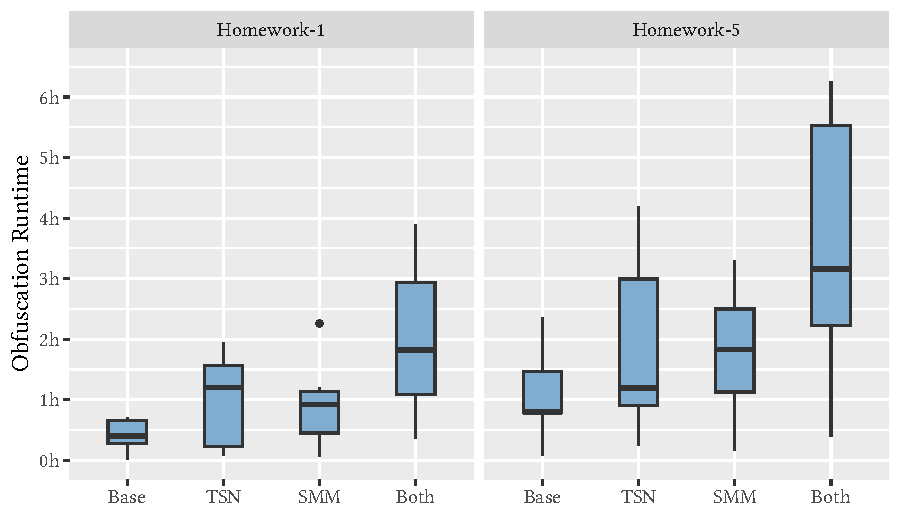
\includegraphics[width=\linewidth]{figures/disseval/eval-MOSSad-runtime_h.pdf}
\caption[Evaluation Results: Obfuscation Duration]{Required obfuscation duration per program for \mossad to reach an obfuscation threshold of 25 percent (for programs with original sizes of \textasciitilde105 LoC for Hw.-1 and \textasciitilde123 LoC for Hw.-5).}
\label{fig:stage5-result-time}
\end{figure}

\begin{figure}[p]
\centering
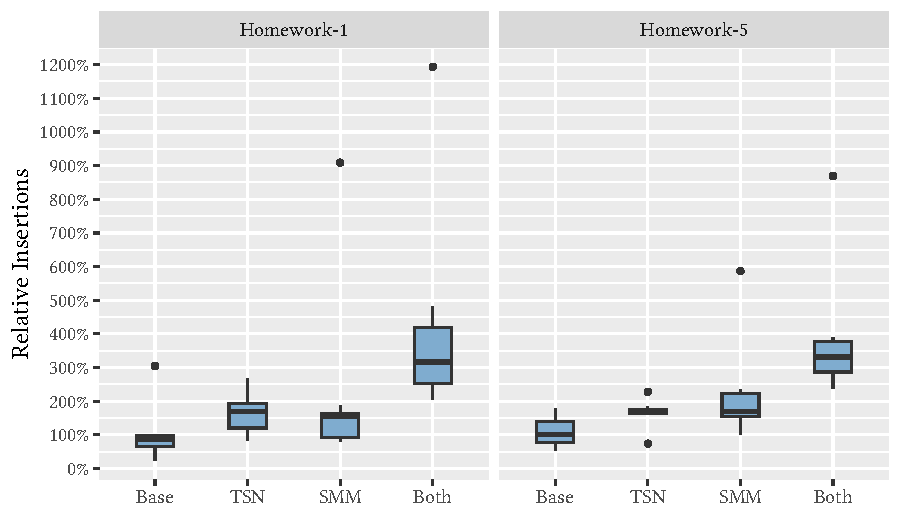
\includegraphics[width=\linewidth]{figures/disseval/eval-MOSSad-insert.pdf}
\caption[Evaluation Results: Inserted Statements]{Required relative insertion of statements for \mossad to reach a 25 percent obfuscation threshold (relative insertions compared to the original program size to normalize for program size).}
\label{fig:stage5-result-loc}
\end{figure}

\section{Result Summary}\label{sec:result-summary}

Our evaluation demonstrates the effectiveness of the proposed defense mechanisms against various obfuscation attack types and their minimal impact on unrelated programs. The results are summarized as follows:

\begin{description}[style=unboxed, leftmargin=0cm]
    \item[Effect on False Positives (\autoref{sec:eval-unrel}):] The defense mechanisms have negligible effects on unrelated programs, ensuring the false-positive rate remains practically insignificant.
    
    \item[Insertion-based Obfuscation (\autoref{sec:eval-insert}):] Token sequence normalization achieves near immunity against insertion-based attacks, with median similarity improvements up to 99.65 percentage points. Subsequence match merging also improves resilience significantly, and combining both mechanisms provides optimal results.
    
    \item[Alteration-based Obfuscation (\autoref{sec:eval-alter}):] Subsequence match merging effectively mitigates alteration-based attacks, achieving median similarity improvements up to 42 percentage points and enabling strong separation of plagiarized and original programs.
    
    \item[Refactoring-based Obfuscation (\autoref{sec:eval-refactor}):] Token sequence normalization minimally impacts refactoring-based attacks, as expected. However, subsequence match merging significantly improves detection, and combining both mechanisms achieves enhanced separation of plagiarized and original programs, with median improvements of up to 22 percentage points.
    
    \item[GPT-4-based Obfuscation (\autoref{sec:eval-gptobf}):] Token sequence normalization has no positive or negative impact on AI-based obfuscation. Subsequence match merging significantly improves resilience against AI-based attacks, with median similarity improvements of up to 19 percentage points. Combining token sequence normalization and subsequence match merging shows similar improvements without drawbacks.
    
    \item[GPT-4-generated Programs (\autoref{sec:eval-gptgen}):] Despite our defense mechanisms not being tailored for AI-generated program detection, we observe improved detection rates. Token sequence normalization has no positive or negative impact on detecting AI-generated programs. Subsequence match merging provides significant improvements, with a median similarity increase of 6.5 percentage points, highlighting its adaptability.
    
    \item[Threshold-based Plagiarism (\autoref{sec:eval-mossad}):] The defense mechanisms substantially increase the computational cost of threshold-based obfuscation, prolonging obfuscation time up to 6 hours per program and inflating program size by up to 1300\%, making such an obfuscation method more tedious and also easily detectable with via metrics such as program size or number of tokens.
\end{description}


In summary, our evaluation demonstrates that the proposed defense mechanisms are highly effective across a range of automated obfuscation attacks.
The proposed defense mechanisms provide significantly (statistical and practical significance) improved obfuscation resilience without any practically significant change in false-positive rates.

\section{Discussion}\label{sec:eval-discussion}%\todo{general content: What do the results mean? What can we show? What is our approach good for? Where do its capabilities end?}
In the following, we discuss the interpretation of the evaluation results and highlight key takeaways for software plagiarism detection.
First, we discuss insights regarding the feasibility of the evaluated obfuscation attacks.
Second, we discuss the broad obfuscation resilience our defense mechanisms provide and the relation to our threat model.
Third, we address the issue of outliers and the remaining overlap between plagiarism instances and unrelated programs in detection results and emphasize the importance of human inspection.
Third, we discuss the preservation of program behavior in obfuscation attacks, focusing on the differences between semantic-preserving and semantic-agnostic attacks and how these affect the effectiveness of plagiarism detection.
Next, we analyze the challenges of AI-based plagiarism and explore the effectiveness of AI-based obfuscation and fully generating programs, stressing the need for future re-evaluation.
Finally, we discuss the benefits of layering defense mechanisms, highlighting how integrating multiple approaches enhances obfuscation resilience.

\subsection{Feasibility of Obfuscation Attacks}
Our evaluation results offer key insights into the effectiveness of automated obfuscation techniques against plagiarism detection systems that do \textit{not} include defense mechanisms.

Insertion-based obfuscation is a highly effective strategy, as it significantly hinders the detection of plagiarized programs by adding semantically irrelevant code. Our baseline results show that this method can completely obfuscate plagiarism instances, underscoring the vulnerability of traditional detection systems to this attack type.
%
Refactoring-based obfuscation further exemplifies the challenges posed by obfuscation attacks. Restructuring the program while maintaining its original behavior effectively reduces similarity measures. The baseline results indicate a limited ability to separate plagiarism pairs from unrelated originals, confirming the efficacy of this obfuscation approach.

AI-based obfuscation introduces additional complexity, as AI-based tools are widely available. However, the results reveal significant variability in the effectiveness of these obfuscation attempts, which appears to depend more on the characteristics of the dataset than on prompt design or programming language. While AI-generated obfuscation is powerful, its reliability is lower than that of algorithmic methods, as evidenced by the high variance across datasets. Nevertheless, the semantic-agnostic nature of AI-based obfuscations presents an increasingly relevant challenge to traditional detection systems, emphasizing the need for more sophisticated countermeasures.

AI-generated programs present an emerging challenge. \textit{Currently}, it is only effective for smaller programs. Our results suggest that AI-generated programs exhibit increased similarity to each other compared to human-written programs, which could facilitate detection if multiple students utilize the same model.
The inability to guarantee preserved behavior in AI-generated programs makes them semantic-agnostic.
While not explicitly designed to address this scenario, the findings reveal that subsequence match merging can improve the separation of AI-generated programs from human-written ones.

Threshold-based obfuscation is a unique form of attack that only terminates upon reaching a pre-defined similarity threshold. Although this approach is effective, it inflates the size of programs to obfuscate them, even when targeting detection systems without any defense mechanisms.


\subsection{On Providing Broad Obfuscation Resilience}

The evaluation shows that our approach improves obfuscation resilience for all employed attacks and datasets. As expected, the \textit{degree} of those improvements depends on the type of obfuscation attack. Nevertheless, when employing our defense mechanisms, we demonstrate that the provided resilience is not limited to a specific obfuscation attack. 
We demonstrated effectiveness against various obfuscation attacks, including both algorithmic and AI-based attacks, encompassing semantic-preserving and semantic-agnostic obfuscation.
Furthermore, we evaluate datasets across different programming languages, in addition to diverse assignment types and sizes, thus demonstrating its adaptability.
In total, we use six datasets in combination with five distinct obfuscation attack types. Moreover, each attack type involves various modifications. For example, refactoring-based obfuscation includes multiple transformation types, while AI-based obfuscation involves 15 varying prompts to generate diverse plagiarism instances.

The five obfuscation attack types used in our evaluation align with the different categories outlined in \autoref{fig:clone-types} and discussed in \autoref{sec:threatmodel-categorization}.
For instance, insertion-based obfuscation represents a structural attack, while our alteration-based obfuscation simulates data-based, structural, and complex attacks. Refactoring-based obfuscation falls under the complex attack category. AI-based obfuscation, depending on the specific prompt used, predominantly results in complex attacks. However, some prompts encourage partial replacement of an implementation, placing them in the category of re-implementation. Moreover, detecting AI-generated programs is fundamentally the same problem as detecting re-implementations and, therefore, also falls into this category.

Our contributions enable token-based plagiarism detectors to achieve broad obfuscation resilience across these categories, which was not possible before.
Specifically, as demonstrated by the evaluation results, this includes complete immunity to lexical and data-based attacks, near immunity to structural attacks, strong resilience to complex attacks, and partial resilience to selective re-implementation.

Our evaluation showed that our contributions provide broad resilience against automated obfuscation attacks on programming assignments by systematically covering these different categories of obfuscation attacks. The smallest improvement was observed for AI-based obfuscation, which is expected, given that this is a semantic-agnostic attack using highly challenging prompts, including partial implementations. Detecting partial implementations is particularly difficult for plagiarism detectors as they must carefully balance between detecting re-implementation and avoiding false positives.
On the other hand, the strongest improvement was observed for structural attacks, which is a significant result. Structural attacks are among the easiest to automate, even with traditional methods, and they tend to consistently affect plagiarism detectors. Thus, improving resilience in this area is crucial for the effectiveness of detection tools.


\subsection{Outliers and Remaining Overlap}

Except for insertion-based obfuscation (see \autoref{fig:stage1-results}), where our defense mechanisms completely eliminate \textit{any} overlap between plagiarism instances and unrelated programs, the evaluation results demonstrate minor overlap. This raises an important question regarding the expectations one should have concerning the quality of plagiarism detection.

In practical terms, some overlap among outliers is not a significant concern. It is essential to recognize that no plagiarism detection tool is perfect. Thus, educators must accept that human inspection is always the final step in plagiarism detection and that no one should solely rely on the results of an automated tool without first verifying the flagged candidates themselves. 
%educators must accept that there will always be a possibility of false positives—instances where unrelated programs are mistakenly flagged as suspicious. Nevertheless, these false positives are not common.

Furthermore, it is crucial to note that plagiarism detectors compare pairs of programs instead, and thus, plagiarize might be included in multiple comparisons. This means that detecting every plagiarism pair is not necessary to identify all students involved in plagiarism. In practice, educators would be presented with a ranked list of suspicious pairs, which includes both unrelated pairs and plagiarism pairs.

As an example, in our evaluation of GPT-4-generated programs, it is not necessary to identify all 1,225 pairs of AI-generated programs to detect each of the 50 generated programs at least once.
Notably, when both of our defense mechanisms are enabled (\textit{Both} in \autoref{fig:stage4-results}), only the first 158 pairs (which is the top 0.07 percent out of all 220,780 analyzed pairs) need to be inspected to successfully identify 90 percent of the AI-generated programs at least once. To detect all 50 AI-generated programs, the first 711 pairs need to be checked, which is the top 0.3 percent of all pairs, underscoring that a small overlap between the pairs of unrelated programs and the plagiarism pairs is not a cause for concern.

Ultimately, it is important to emphasize that no plagiarism detection tool can provide 100 percent certainty. Therefore, human inspection and informed decision-making are essential in ensuring fair and accurate investigation of misconduct. Educators must \textit{always} engage in thoughtful analysis of the results generated by these tools to effectively discern genuine cases of plagiarism from false positives.

\subsection{Preservation of Program Behavior}

In our evaluation, we employed both semantic-preserving and semantic-agnostic attacks. The former category ensures that program behavior remains intact, while the latter attempts to preserve behavior without providing any guarantees. Notably, AI-based obfuscation attacks, such as those generated by GPT-4, fall into the latter category, where there are no assurances that the program behavior does not change.

For this particular obfuscation attack, we generated a total of 300 plagiarism instances across four datasets, with 75 instances each. Given the scale of our evaluation, it is impractical to verify that these instances did not alter program behavior. While GPT-4 is a sophisticated model, we anticipate that some cases may deviate in behavior. However, this aspect does not undermine our results; instead, it strengthens them. Semantic-agnostic attacks impose fewer constraints, allowing for more substantial changes and a wider variety of alteration types. Consequently, these attacks present a more significant challenge to defend against. Thus, it is noteworthy that our defense mechanisms provide significantly improved resilience for these attacks, even though they are primarily designed to target semantic-preserving attacks.

Under the circumstances of our evaluation, verifying the behavior of the semantic-agnostic plagiarism instances is, therefore, unnecessary. In practical scenarios, students typically strive to maintain the intended behavior of their programs to avoid penalties or lower grades. Therefore, while semantic-altering obfuscation attacks remain an area for future work, the current findings demonstrate the resilience of our defense mechanisms against a variety of obfuscation techniques, including semantic-preserving and semantic-agnostic attacks.


\subsection{AI-based Plagiarism}\label{sec:discussion-ai}
AI-based attacks~\cite{Biderman2022}, particularly those utilizing generative AI, present a growing concern for plagiarism detection.
We discussed two possible scenarios when employing generative AI to cheat on programming assignments. \textit{Automatic obfuscation} of an existing solution and \textit{fully generating} solutions from the assignment description.
%
Based on our evaluation results, automatic obfuscation is \textit{currently} the more effective approach for medium and larger assignments, as fully generating only works well for smaller programs. Generated programs do not fulfill necessary functional requirements (not implementing the required behavior precisely) and even non-functional requirements like code style, thus requiring significant manual effort to improve them sufficiently.
Automatic obfuscation resembles human obfuscation practices, as a pre-existing solution is altered while \textit{trying} to preserve the program behavior.
For both approaches, our defense mechanisms have shown improved resilience.

For AI-generated solutions, there's an ongoing debate on whether this form of cheating\footnote{Obviously, it only constitutes \textit{cheating} if using generative AI is explicitly not allowed in the course.} qualifies as plagiarism~\cite{Novak2019, Saglam2024a}.
Our approach improves the detection rate by helping to recognize the similarities among generated solutions that occur due to the semi-deterministic nature of large language models.
This improvement is surprising, as our defense mechanisms are \textit{not} designed to detect AI-generated programs.

\subsubsection{On the Effectiveness of AI-based Obfuscation}

Our evaluation results show that the effectiveness of our defense mechanisms for AI-based obfuscation is less pronounced compared to their performance against algorithmic attacks. This can be attributed to two key factors.

First, the overall varying effectiveness of AI-based obfuscation plays a significant role. Our results indicate a strong variance in the similarity values achieved by AI-based obfuscation. While part of this variability can be explained by the different prompts used in our evaluation, this trend remains consistent even when examining the results for each prompt individually (see \autoref{fig:stage3-results-byprompt}). For plagiarized programs that already exhibit a high degree of similarity to their original versions, there is limited potential for our defense mechanisms to increase that any further.

Second, generative AI employs a much broader range of modifications compared to algorithmic obfuscation techniques. Algorithmic methods typically rely on a well-defined, limited set of changes during obfuscation. Even refactoring-based obfuscation, which involves multiple refactoring operations, operates within a constrained set of transformations. In contrast, AI-based obfuscation introduces a far more diverse range of modifications, even when using the same prompt. In our evaluation, we observed strong variations in the types of changes applied by AI depending on both the prompt used and the dataset involved. These diverse modifications alter token sequences extensively, posing a challenge to our defense mechanisms.

Nonetheless, it is important to note that our evaluation still shows a notable improvement in resilience against AI-based obfuscation, even in the presence of these complex and varied changes. This demonstrates that while AI obfuscation is an effective technique, our defense mechanisms mitigate its effects.

Interestingly, the effectiveness of AI-based obfuscation attacks strongly varies depending on the dataset used. As illustrated in \autoref{fig:stage3-results}, AI-based obfuscation performs well for Homework-1, while it does not perform well for both PROGpedia datasets. TicTacToe and Homework-5 achieve mixed results. The median similarity differences range, depending on the dataset, between around ten and around 78 percentage points (see \autoref{tab:diff-gpt-obf}).

Although the evaluated plagiarism instances proved to be effective, the process of generating them was not straightforward.
In some cases, GPT-4 produces incomplete or invalid code. Sometimes, the obfuscated programs did not compile, thus requiring re-generation.
%For three original programs, we were not able to produce an acceptable result even after more than 50 attempts.
Despite over 50 attempts, we could not produce a valid result for three original programs, which all exceeded 300 LOC.
%
Thus, algorithmic obfuscation \textit{currently} exhibits more consistent results than AI-based obfuscation, and \textit{currently} can be just as effective.
%However, AI-based obfuscation produces a wide variety of modifications, which could aid in avoiding detection during manual inspection.
However, AI-based obfuscation is more useful in avoiding detection during manual inspection, as it produces diverse modifications and can imitate human-made code.

\subsubsection{On the Effectiveness of AI-based Generation}

While AI-based generation works to a certain extent, its effectiveness is \textit{currently} limited. 
The programs generated entirely by GPT-4 did not fully comply with the specific requirements of the programming assignments, often resulting in additional output or slightly altered behavior.
These discrepancies suggest that fully AI-generated solutions may only be suitable for smaller, less complex assignments.
In our case, the TicTacToe dataset, with a size of approximately 236 lines of code, appears to be near the threshold where fully generated solutions start to exhibit these inconsistencies.

A noteworthy observation is that AI-generated programs are typically shorter than those created by human developers, especially within the TicTacToe dataset. This reduction in length may contribute to the higher degree of similarity observed between AI-generated solutions. While large language models like GPT-4 are not entirely deterministic, they exhibit a level of determinism sufficient for software plagiarism detection purposes. This inherent determinism, coupled with the more concise code produced by AI, may explain why AI-generated programs tend to resemble each other more closely than human-generated ones.

Finally, GPT-4 has a tendency to produce placeholder comments instead of fully implementing certain methods, particularly when the task or method is not well-defined in the prompt. This behavior further limits the effectiveness of AI-based generation for complex assignments, as these incomplete implementations require additional manual intervention to complete.

\subsubsection{Emerging Threats}

While our results thus show that our contributions can effectively address \textit{current} threats of artificial intelligence, rapid advancements in this field may necessitate future re-evaluation. In the future, AI-based obfuscation methods may exhibit less variance in their effectiveness, thus increasing their reliability.
Similarly, new algorithmic attacks might emerge.
%
However, as discussed in our threat model, all emerging attacks must affect the same attack surface (see \autoref{sec:threatmodel-analysis}). Thus, subsequence match merging will provide resilience to emerging attacks. However, the degree of that resilience remains to be assessed.

The rapid development in the field of generative AI may lead to emerging threats that warrant close attention~\cite{Lancaster2023}. One area of particular concern is AI-generated programs. As generative AI advances, this might become feasible for larger programs and produce functionally correct programs for more complex assignments.
%
To detect such fully generated programs, detection systems need capabilities to detect obfuscation via implementation, which can be considered semantic clones. Here, caution is warranted. While matching full re-implementations seems desirable, it risks introducing significant false positives by flagging unrelated programs created independently by students. Note that unrelated solutions to a single problem can also be seen as semantic clones. Thus, we see the danger of creating unreliable detection systems, which may lead to unfairly penalizing students. Addressing re-implementation or semantic clones, therefore, raises philosophical questions about the boundaries of what type of plagiarism we actually want a detection system to target.

For fully generated programs, for example, via generative AI, plagiarism detection methods may not be sufficient for emerging attacks.
If traditional plagiarism detection methods, including the defense mechanisms evaluated in this dissertation, prove inadequate against more sophisticated AI-generated code, alternative techniques may need to be explored~\cite{karnalim2024}. One research area is the development of AI-based detectors that act as countermeasures to generative AI. However, at present, such AI-based detectors have not demonstrated sufficient reliability or performance, and they remain an area of ongoing research~\cite{WeberWulff2023, Pan2024, Khalil_Er_2023}. Another possibility lies in signature- or watermark-based methods, where the artifacts generated by AI are always identifiable as such. This approach would involve recognizing specific patterns or characteristics inherent to AI-generated content, allowing for consistent identification, regardless of the obfuscation techniques applied. Again, this is ongoing research~\cite{zhao2024provable, Jiang2023}. 
%
It is important to note, however, that these potential future developments lie beyond the scope of this dissertation and even outside of the research area of software plagiarism detection.


\subsection{Layering Defense Mechanisms}
Attack-specific defense mechanisms are highly effective, as they can be tailored with strong assumptions about specific obfuscation techniques in mind.
For their targeted obfuscation attacks, attack-specific mechanisms outperform attack-independent approaches.
This is evident in the case of token sequence normalization in \autoref{fig:stage1-results}, where the defense mechanism fully separates plagiarism pairs from original pairs, completely outperforming subsequence match merging.

However, attack-specific mechanisms mostly focus solely on a single known obfuscation attack type. Multiple attack-specific mechanisms must be combined to achieve broad resilience.
Additionally, attack-specific mechanisms can only be designed for known attacks and may not be equipped to handle emerging threats, as they rely on assumptions that may not hold true for unknown obfuscation techniques.

Attack-independent mechanisms, such as subsequence match merging, make fewer assumptions about the obfuscation techniques in use. Thus, they provide less resilience for a given obfuscation attack. 
Their strength, however, lies in providing broad resilience.
Throughout our evaluation, we observed that subsequence match merging consistently offered resilience across a variety of obfuscation attacks.
Because of its heuristic nature and the fact that it operates at a high level of abstraction, it can provide \textit{some} resilience against unknown and emerging obfuscation attacks\footnote{As discussed in \autoref{sec:threatmodel-analysis}, all obfuscation attacks need to affect the token sequence, thus interrupting the subsequence matching, to have any effect on a token-based plagiarism detector.}
Attack-independent approaches are essential for defending against emerging threats.
Since they make fewer assumptions about the nature of incoming obfuscation attacks, they offer a level of protection against unknown attacks that attack-specific mechanisms may not.

The ideal solution is to combine multiple defense mechanisms, leveraging both attack-specific and attack-independent defense mechanisms.
This strategy provides targeted resilience against well-known or highly effective obfuscation attacks while also offering broad protection against unknown or emerging techniques.
Layering multiple defenses is a well-established strategy in information security and risk assessment, often referred to as the \textit{Swiss cheese model}~\cite{Reason1990} or \textit{defense in depth}~\cite{Stytz2004, Lippmann2006, Anderson2020}.

When using this layered approach, it is critical to ensure compatibility between defense mechanisms to avoid unintended side effects that could reduce overall obfuscation resilience or detection quality.
In the context of software plagiarism detection, it is beneficial to allow users to enable or disable different defense mechanisms depending on their needs or to mitigate potential side effects\footnote{We integrated our defense mechanism into JPlag, allowing educators to benefit from their obfuscation resilience. When using them, it is possible to toggle them as needed for exactly those reasons.}.

Our defense mechanisms are designed to be minimally intrusive, enabling them to be layered with other approaches.
In our evaluation, we examine the combination of defense mechanisms to check for adverse side effects.
While, in some cases, individual mechanisms outperformed combinations, the overall drawbacks of combining them are insignificant.
Therefore, our mechanisms can be safely used in a layered defense strategy.

\section{Threats to Validity}
We now discuss how we address threats to the validity of our evaluation, following the guidelines outlined by \citet{Wohlin2012} and \citet{runeson2008}. These threats apply to the first goal of our evaluation, where we assess obfuscation resilience for programming assignments (\gref{1}). By identifying and mitigating potential threats to internal, external, and construct validity and reliability, we ensure that our findings accurately reflect the effectiveness of our defense mechanisms against automated obfuscation attacks.

\subsection{Internal Validity} 
Internal validity refers to whether there are influences that can unknowingly affect the analyzed variable with respect to causality~\cite{Wohlin2012}.
%

    \textbf{Baseline Consistency:} For internal validity, we used JPlag as a baseline but also implemented our defense mechanism for JPlag, ensuring that all other conditions remained constant when comparing the defense mechanism with each other or with the baseline. 

    \textbf{Handling of invalid programs:} Some public datasets contain invalid or incomplete programs (e.g., programs that do not compile), which could lead to inaccurate results if not properly handled. We addressed this by preprocessing the datasets and removing programs that do not compile. However, even if some cases still remain in the datasets, they do not affect the observed results, as we use the same datasets for the baseline and all of our approaches. 

    \textbf{Validity of the Labeling:} The labels of plagiarism instances in public datasets are often incomplete, incorrect, or solely based on tools like JPlag, which could introduce bias. This threat does not apply in our evaluation, as we use automated obfuscation to generate plagiarism instances (via existing plagiarism generators, obfuscation attack implementation, and large language models). Thus, we have exact labels. As a preprocessing step, we carefully filtered out instances of human plagiarism based on the labels, analyzed them with JPlag, and performed human inspections.

\subsection{External Validity}
External validity concerns the extent to which our findings can be generalized beyond the specific context of the evaluation. % to what extent it is possible to generalize the findings, and to what extent they are of interest to others

    \textbf{Generalizability across datasets:} The datasets used in this evaluation are real-world student submissions from various university courses, thus representing typical scenarios for software plagiarism detection.
    The number and size of programs in the datasets, as well as the choice of programming language, conforms to the typical application of software plagiarism detection, as confirmed by the JPlag developer survey (see \autoref{sec:survey}) and the relevant literature~\cite{Novak2019}.
    We used diverse datasets from different courses, two programming languages, and assignment sizes to improve generalizability and ensure a representative evaluation. This could have been further improved by including a suitable dataset of Python programs, which was not possible due to unavailability. 

    \textbf{Generalizability of obfuscation attacks:}
    Limiting the evaluation to only a few types of obfuscation attacks could hinder the applicability of our results to broader contexts. To enhance external validity and thus ensure that our findings are generalizable, we included a diverse set of obfuscation techniques from all categories outlined in our threat model (see \autoref{sec:threatmodel-categorization}). Note that these are (with the exception of simulated alteration) real-world obfuscation attacks that are, directly or conceptually, available in practice. These steps ensure that our results are relevant to real-world obfuscation threats.

    \textbf{Tool Independence:} Our defense mechanisms are tool-independent, enabling use in token-based and even some other structure-based plagiarism detectors, enhancing their general applicability.
    We evaluated our defense mechanism only using JPlag as the baseline, as other tools are either not applicable to all datasets, closed-source, or provide restricted results. However, this is not a threat to generalizability, as JPlag is considered state-of-the-art~\cite{Novak2019, Aniceto2021} and operates similarly to other widely used tools, reinforcing the generalizability of our findings.

    \textbf{Influence of Prompt Quality:} To address the impact of prompt choice for AI-based obfuscation, we performed systematic "\textit{prompt-engineering}" prior to the evaluation. We then evaluated with 15 suitable different prompts. We generated multiple plagiarism instances for each prompt, which we repeated for multiple datasets. While the impact of the prompt varies (see \autoref{fig:stage3-results-byprompt}), the variation is not strong enough to obscure the overall trend. Thus, we observe consistent patterns of obfuscation resilience across prompts, supporting the generalizability of our results.

\subsection{Construct Validity}
Construct validity refers to how well the evaluation measures its intended purpose and whether the metrics and baselines chosen are appropriate. Thus, it refers to the degree to which we measure theoretical construct we intend to measure.

    \textbf{Evaluation Methodology Alignment:} To enhance construct validity, we aligned our evaluation methodology with those from established and related research works. This ensures that our approach is consistent with the standards in the field. While we deviate from related works by not using a threshold-based classification, we do so specifically to improve internal validity (see \autoref{sec:metrics}), as this method is fundamentally flawed. Finally, we employ an approach-independent ground truth, use established similarity metrics, and a Goal-Question-Metric plan~\cite{Basili1984, Basili1992}.

    \textbf{Underlying Research Object:} We ensure consistency between theoretical research objects and the measurements by maintaining their direct alignment. Since our study evaluates the resilience of software plagiarism detectors against automated obfuscation attacks, we use the similarity scores generated by the detectors as our primary measurement. Additionally, to assess automated obfuscation accurately, we directly utilize real-world plagiarism generators such as \mossad and GPT-4 (which can be exploited to act as one) in our evaluation.
    
    \textbf{Choice of Baseline:} The baseline selection might affect the comparison and outcomes. We addressed this by selecting JPlag as the baseline, as it is widely recognized as a state-of-the-art tool~\cite{Aniceto2021, Novak2019}, ensuring that the comparison is relevant and accurate. As previously mentioned, it operates similarly to other widely used tools by employing standard similarity metrics.

\subsection{Reliability}
Reliability concerns the consistency of the results and whether the study can be replicated under the same conditions.
To ensure reliability, we provide a comprehensive reproduction package for our evaluation~\fancycite{replication-package}.

    \textbf{Use of Internal Datasets:} Using internal datasets can hinder reproducibility. To enhance reliability, we used both public and internal datasets, balancing generalizability with the need for open data where possible. We discussed any preprocessing steps and the employed obfuscation attacks for all datasets.
    For the internal datasets (TicTacToe and BoardGame), we provide raw results and metadata in our replication package. 
    
    \textbf{Consistency across evaluations:} Different datasets vary in size, language, and type of program, which could lead to inconsistent results. We addressed this by using uniform preprocessing steps, evaluation metrics, and statistical tests across all datasets, ensuring that the evaluation was consistent regardless of dataset type or complexity.

    \textbf{Publishing of Obfuscation Attacks:}  The obfuscation attacks utilized in our study can be considered malware, which restricts our ability to provide access to these tools. The exception is GPT-4~\cite{gpt4}, which is publicly available; however, we do not provide a detailed, step-by-step guide on exploiting it for plagiarism detection. While omitting these artifacts or details may hinder reproducibility, balancing this limitation with ethical considerations and the responsibility regarding potential misuse. We aim to ensure that our findings can be reliably assessed while maintaining a commitment to ethical standards.


\chapter[Evaluating Modeling Plagiarism]{Evaluating Plagiarism Detection for Modeling Assignments}\label{sec:mde-eval}

This chapter evaluates our approach to enabling token-based plagiarism detection for modeling assignments (\contribution{2}) with datasets from real-world modeling assignments. Thus, it addresses our first evaluation goal (\gref{2}).
We thus show the feasibility of applying token-based techniques for detecting modeling plagiarism and that they provide obfuscation resilience, outperforming the state-of-the-art.
We demonstrate our approach's effectiveness in detecting plagiarism based on algorithmic, AI-based, and human obfuscation.
Our results show that our approach provides resilience against automated obfuscation attacks.
%
We implemented our approach based on JPlag~\cite{prechelt2002}. In contrast to the evaluation for code in \autoref{cha:code-eval}, JPlag is thus not the baseline, as we evaluate whether we succeeded in enabling token-based plagiarism detection for artifacts of modeling assignments.
Instead, we use the LSH-based approach of \citet{Martinez2020} as a baseline.
For our implementation based on JPlag, we used the default minimal match length of 7.
For the remainder of this chapter, we use \textit{Token-based} as the identifier for our approach.
For the LSH-based approach, we used the recommended parameters for \ac{EMF} metamodels.
We avoided any parameter tuning to ensure a fair comparison.
%
Note that this evaluation stage only includes the defense mechanism for modeling languages: model subtree reordering (MSR).
To analyze the effects of MSR, we evaluate our approach with \textit{and} without it.
%, subsequence match merging, and a combination of both. The second evaluation stage covers the mechanisms that apply to modeling languages.

Our approach demonstrates broad resilience to algorithmic obfuscation attacks, clearly distinguishing between plagiarism pairs and unrelated originals. Notably, the approach of \citet{Martinez2020} shows vulnerability for renaming-based obfuscation. For human-obfuscated plagiarism, our method consistently achieves effective separation from unrelated pairs, outperforming the approach of \citet{Martinez2020}, which struggles with detection. Against AI-obfuscated plagiarism, our method achieves high similarity scores, especially in complex plagiarism-to-plagiarism comparisons, thus outperforming \citet{Martinez2020}. We provide a replication package for replicability~\fancycite{replication-package}.

The chapter is structured as follows: First, we introduce the obfuscation attacks used for evaluation. Next, we evaluate plagiarism modeling based on algorithmic obfuscation, manual obfuscation by novice modelers, and AI-based obfuscation using ChatGPT~\cite{ChatGPT}. After that, we summarize the results. Finally, we discuss threats to validity.

\ownpublications{
    \fancycite{Saglam2024a},
    \fancycite{Saglam2023}, and
    \fancycite{Saglam2022}.
}

\section{Obfuscation Attacks}
The following discusses the obfuscation attacks used for our modeling plagiarism evaluation.
In essence, we use three automated obfuscation categories: Manual, algorithmic, and AI-based. For manual obfuscation, we use models obfuscated by novice modelers (see \autoref{sec:human-plagiarism}).
We base the algorithmic obfuscation on existing works from model clone detection~\cite{Babur2019} and model refactoring~\cite{Bettini2022, Sidhu2018, Stoerrle2015}.
Finally, for AI-based obfuscation, we used twelve different prompts, leading to various model changes.

In total, we employ six categories of obfuscation attacks to evaluate modeling plagiarism (note that each category consists of multiple obfuscation types):
%We evaluate in three stages: %, according to which our evaluation is structured into two parts.
\begin{enumerate}
\small
%[style=unboxed,leftmargin=0cm,topsep=2pt]
%\begin{enumerate}[style=unboxed,leftmargin=0cm]
\item Insertion of new model elements at random valid positions in the model.
\item Random deletion of existing model elements and their children (semantic-altering).
\item Random intra- and inter-reference reordering of model elements (semantic-preserving).
\item Renaming of random elements to pseudo-sensical names based on existing names.
\item Manual, mixed-technique obfuscation by novice modelers (semantic-preserving).
\item AI-based obfuscation via ChatGPT with mixed prompts (semantic-agnostic).
%\item[S1] Evaluation for isolated attack types.
%\item[S2] Evaluation for manual plagiarism by novice modelers.
%\item[S3] Evaluation for AI-obfuscated plagiarism by ChatGPT.
%\item[S3] Evaluation for fully AI-generated plagiarism by ChatGPT
%\end{enumerate}
\end{enumerate}
Note that attack types 1. and 4. \textit{could} be considered semantic altering due to the algorithmic and randomized nature of the obfuscation attack implementation. However, this characteristic only enhances the robustness of the evaluation results, as these attacks are considered even more effective.
As discussed in \autoref{sec:mde-intrusiveness}, defining semantic-preserving obfuscation in the context of models is not as straightforward as for code. For non-executable models without formally defined semantics, intrusiveness depends on the use case.
In the context of modeling assignments, semantic-preserving obfuscation attempts to ensure that the modified model still qualifies as a valid solution, thus maintaining the same concepts.

\textbf{Algorithmic Obfuscation:}
We evaluate the first four obfuscation attacks (\textbf{1.} to \textbf{4.}) in one evaluation stage, as they are all randomization-based algorithmic obfuscation techniques. A crucial benefit of these single-type obfuscation attacks is that they allow comparisons of which types of changes a plagiarism detection system is resilient against.

We base the algorithmic obfuscation techniques on existing works from model clone detection~\cite{Babur2019} and model refactoring~\cite{Bettini2022, Sidhu2018, Stoerrle2015} and on our observations during the experiment with novice modelers described in \autoref{sec:human-plagiarism}. There are some similarities to obfuscation in code plagiarism~\cite{Karnalim2016}, but many of the employed modifications are modeling-specific.
%
We omit trivial attacks (Type-A~\cite{Babur2019}, L0/L1~\cite{Karnalim2016}) like verbatim copying, attacks against which our approach and the LSH-based approach are inherently resilient. This includes attacks like changing the type of attributes, the multiplicity of references, and trivial name changes like typographical errors.
We also omit attacks that do not affect our approach or the one of \citet{Martinez2020}. This includes, for example, the modification of enumerations, annotations, default values, \textit{ordered} or \textit{unique} constraints, or generics.

\begin{table}[b]
	\centering
	\begin{tabular}{l c c c c c c c c}
		\toprule
		Attack & 
		\multicolumn{1}{l}{\rlap{\rotatebox{45}{\small{Package}}}} & \multicolumn{1}{l}{\rlap{\rotatebox{45}{\small{Class}}}} & \multicolumn{1}{l}{\rlap{\rotatebox{45}{\small{Operation}}}} & \multicolumn{1}{l}{\rlap{\rotatebox{45}{\small{Attribute}}}} &
		\multicolumn{1}{l}{\rlap{\rotatebox{45}{\small{Reference}}}} & \multicolumn{1}{l}{\rlap{\rotatebox{45}{\small{Supertype}}}} &
		Level  & Type \\
		\midrule
		Insert Element   & \checkmark & \checkmark & \checkmark & \checkmark & \checkmark & \checkmark & L2.5, L3, L4 & B, C \\
		Delete Element   & --         & \checkmark & --         & \checkmark & \checkmark & \checkmark & --           & B    \\
		Reorder Elements & \checkmark & \checkmark & --         & \checkmark & \checkmark & --         & L2.5, L3     & B, C \\
		Rename Element   & \checkmark & \checkmark & --         & \checkmark & \checkmark & --         & L2, L2.5     & C    \\
		\bottomrule
	\end{tabular}
    \caption[Algorithmic Obfuscation Attacks]{Algorithmic obfuscation attack types employed in this evaluation and their corresponding clone level \cite{Karnalim2016} and type \cite{Babur2019}. Adapted from \cite{Saglam2022}.}
	\label{tab:mde-algo-attacks}
\end{table}%

We executed these obfuscation techniques on different element types, for this \autoref{tab:mde-algo-attacks} gives an overview.
%We executed the modification for each attack on ten random model elements of the same type.
We chose random positions of all possible valid positions for a given element type to insert elements. 
Regarding the insertion of references and supertypes, we referenced random existing classes. Note that insertion, like introducing a new supertype, also affects references. Thus, it is not a pure insertion as in code obfuscation.
%
For deletion, we are limited to deleting existing elements in the models, which also affects potential child elements. For example, deleting a classifier also deletes all contained structural features. Note that this type of attack inherently affects the degree to which a given model correctly fulfills the assignments. However, we still included this attack for completeness.
%
We executed the reordering by moving elements to a randomly chosen position that was valid for the given element type.
This includes both moving elements across containment relations (e.g., moving classes to other packages) and reordering model elements in a single n-ary containment relation (e.g., reordering the attributes of a class). As for deletion, this might affect child elements. Moving a class involves moving all contained features as well.
%
For renaming and the names of inserted elements, we generated realistic names based on the fragments of existing names in the metamodel, which are indistinguishable at first glance. We included renaming, as the LSH-based approach by \citet{Martinez2020} uses names as part of the LSH signatures.

Due to the limited use of operations in the metamodels of our dataset, we only performed insertion for operations.
We also omitted the deletion of packages as this drastically alters the model semantically and is thus not a realistic obfuscation attack.
We also committed some more complex obfuscation types on purpose, as with increased complexity, they can be less frequently applied (see \autoref{fig:clone-types}), thus not altering the tokens sequences broadly, limiting effectiveness.


\textbf{Manual Obfuscation:}
In the second stage, we evaluate with human-made, mixed-technique obfuscation by novice modelers (\textbf{5.}).
We use the dataset introduced in \autoref{sec:human-plagiarism} for this, based on our experiment on modeling plagiarism. These plagiarism instances were created by novice modelers provided with the metamodeling assignment outlined in \autoref{sec:datasets} along with pre-existing solutions from the corresponding dataset. The participants made various changes, with an average of 43.7 changes per participant and a median of 31.5. On average, this corresponds to one change for every two model elements.

Participants frequently performed renaming operations, such as modifying element names or altering their formatting, to obfuscate the model while preserving its structure. Reordering elements within packages or models was another common approach, leveraging the flexibility in the order of multi-valued references. Structural modifications, such as introducing or dissolving packages, altering properties like cardinalities, and inserting and deleting features or classifiers, were also widely used. For details, please refer to \autoref{tab:student-obfuscation}.
%These obfuscation types align with the algorithmic obfuscation in the previous evaluation stage.

\textbf{AI-based Obfuscation:}
Finally, we used plagiarism instances created via AI-based obfuscation with ChatGPT for the last stage (\textbf{6.}). 
As discussed in \autoref{sec:ai-plagiarism}, we investigated fully-generating solutions with ChatGPT. However, since this produced invalid and obviously suspicious models due to the currently limited modeling capabilities of ChatGPT~\cite{Camara2023}, we chose solutions obfuscated by ChatGPT to evaluate our approach and compare it with the state-of-the-art.
Note that this evaluation was done with ChatGPT 3.5, which was, at the time, the most recent available version.
%
We used ChatGPT to generate obfuscated versions of models from the base dataset introduced in \autoref{sec:datasets}.
This method requires little modeling knowledge and produces plagiarism that is well obfuscated and relatively inconspicuous to the human eye.
While using ChatGPT occasionally led to minor syntactical issues, we mainly produced correct models that were obfuscated according to our instructions.
As discussed in \autoref{subsec:chatgpt-obf}, we provided ChatGPT with models from the dataset and applied twelve different prompts for two models to generate a total of 24 plagiarism instances.

Interestingly, the produced modifications are diverse but, more importantly, modeling-specific.
They involved various modifications to the modeling artifacts, altering their structure while maintaining plausibility within the assignment domain. These changes included adding, deleting, restructuring, and reordering elements. Moreover, this involved the manipulation of containment and supertype hierarchies. We observed restructuring models by introducing new superclasses and moving elements into these new classes. Names were altered using abbreviations, synonyms, or domain-specific prefixes and suffixes, while properties like multiplicities were adjusted. Additionally, some changes included the addition of new domain-relevant structures, such as creating a \texttt{Node} class with relationships to existing classes like \texttt{Link} and \texttt{Container}, or deduplicating attributes by introducing abstract superclasses like \texttt{NamedElement}.
%
Most of these transformations appeared natural and plausible, fitting into the context of the assignment. Even when inconsistencies or issues arose, they resembled typical human errors. However, few modifications stood out due to illogical naming conventions or less coherent structural changes.

\section{Algorithmic Obfuscation}

\label{subsec:first-stage}

\noindent
Our first stage demonstrates broad resilience to different types of algorithmic obfuscation attacks.
As discussed, we evaluate the insertion, deletion, rendering, and renaming of model elements.
There, we applied each obfuscation attack 20 times to a randomly chosen human-made model.
In total, four original metamodels were chosen, thus generating 80 plagiarism instances.
This stage is particularly useful to determine how different approaches perform for singular attack types. 

\begin{figure}
\centering
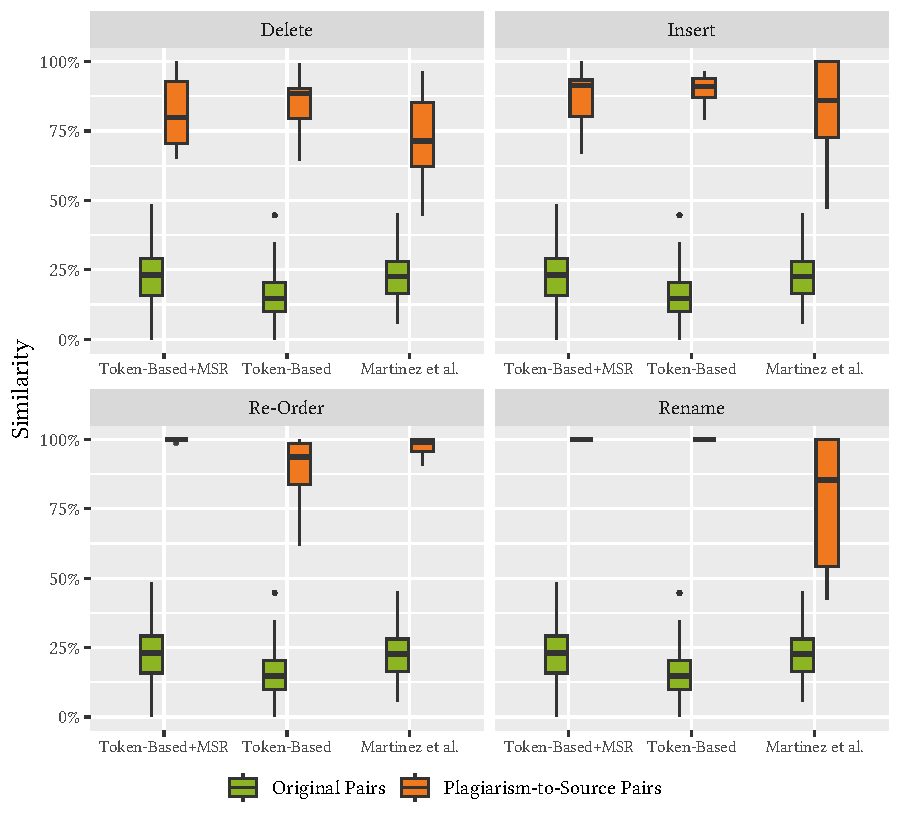
\includegraphics[width=1\linewidth]{figures/disseval2/attacktypes_avg.similarity.pdf}
\caption[Evaluation: Algorithmic Obfuscation of Models]{Results for the attack type evaluation for our token-based approach (Token-Based) with and without MSR and the LSH-based approach by \citet{Martinez2020}.}
\label{fig:attacktypes-results}
\end{figure}


 \subsection{Results}
\autoref{fig:attacktypes-results} shows the results for the different attack types.
% DELETION
For deletion attacks, all approaches can be affected by deleting elements and their children. However, this effect is limited for our approaches, as only few plagiarism instances drop below a similarity of 75\% to their source metamodels. Notably, its effect is larger with MSR enabled.
In contrast, for the LSH-based approach of \citet{Martinez2020}, this is the case for more than half of the plagiarism-to-source pairs. The median value drops below 75\%.
% INSERTION
In contrast to deletion attacks, all approaches are only slightly affected by insertion. Our approaches perform very well, achieving median similarity values above 90\%. The approach of \citet{Martinez2020} performs slightly worse but still maintains a high median value.
However, for insertions and deletions, their approach has some outliers that come close to the similarity values of the original pairs.
% MOVE
For Reordering-based attacks, the approach of \citet{Martinez2020} also performs well, showing little effect of the obfuscation attack.
Our variant without MSR, however, can be affected by reordering attacks, showing only some resilience.
In contrast, with MSR enabled, our approach shows little to no effect on the obfuscation attack. This shows that MSR makes the detection virtually invariant to reordering, thus fulfilling its purpose.
% MOVE
For renaming-based obfuscation attacks, our approaches show complete immunity, which is an inherent trait of token-based approaches.
In contrast, the approach of \citet{Martinez2020} is prone to renaming, showing a $Q_1$ at around 55\%, thus having many pairs close to the unrelated originals. This shows the advantage of token-based approaches.

\begin{table}[b]
	\centering
    \small
	\begin{tabular}{llrrr}
		\toprule
		Obfuscation Type                            & Approach        & $\Delta$ Mean & $\Delta$ Median & $\Delta$ IQR  \\
		\midrule
		\multirow{3}{*}{Delete}                     & Token-Based + MSR     & 60.21  & 59.24    & 42.86 \\
		                                            & Token-Based           & \B{72.28}  & \B{74.01}    & \B{61.90} \\
		                                            & Martinez et al. & 50.14  & 48.72    & 33.98 \\
        \midrule
		\multirow{3}{*}{Insert}                     & Token-Based + MSR     & 65.74  & 68.69    & 51.81 \\
		                                            & Token-Based           & \B{76.32}  & \B{77.05}    & \B{67.60} \\
		                                            & Martinez et al. & 60.74  & 63.28    & 44.43 \\
        \midrule
		\multirow{3}{*}{Re-Order}                   & Token-Based + MSR     & \B{76.09}  & 76.47    & \B{69.77} \\
		                                            & Token-Based           & 73.79  & \B{77.95}    & 62.20 \\
		                                            & Martinez et al. & 75.41  & 76.30    & 67.63 \\
        \midrule
		\multirow{3}{*}{Rename}                     & Token-Based + MSR     & 76.14  & 76.47    & 69.77\\
		                                            & Token-Based           & \B{84.04}  & \B{84.29}    & \B{78.45} \\
		                                            & Martinez et al. & 55.49  & 62.72    & 26.16 \\
		\bottomrule
	\end{tabular}
    \caption[Evaluation: Algorithmic Obfuscation of Models]{Similarity differences between the algorithmically obfuscated plagiarism instances and the unrelated originals (higher means better detection) for the results in \autoref{fig:attacktypes-results}.}
	\label{tab:summary-stats-algo}
\end{table}


\subsection{Discussion}
Note that with limited obfuscation strength, the effects of the normalization are less pronounced, and thus, when looking at the similarity differences (\autoref{tab:summary-stats-algo}), our approach without MSR performs quite well, as our approach with MSR has smaller differences due to the increase for original pairs. As we use a singular obfuscation type with limited modifications in this stage, the possible effects of the normalization are inherently limited.

While deletion-based attacks seem effective on paper, they are not feasible in practice.
Usually, very little can be removed from an assignment's artifact without making the solution incomplete or even plain wrong.
In our evaluation, we randomly removed elements along with their children, which sometimes resulted in removing large subtrees (thus explaining why its effect is slightly stronger with MSR enabled). With that in mind, the effects of these attacks were relatively mild, and our approach still allows differentiation between plagiarism pairs and original pairs. However, the approach of \citet{Martinez2020} is more affected by deletion attacks.

Regarding insertion attacks, our approach shows resilience, while for renaming, our approach demonstrates complete immunity. Without MSR, our approach is prone to reordering-based attacks, which motivates the need for MSR. In contrast, the approach from \citet{Martinez2020} is strongly vulnerable to renaming-based attacks but not vulnerable to reordering attacks.
It is worth noting that renaming and reordering are probably the most trivial attacks, both for humans and computers~\cite{Saglam2023}.

\textit{Overall, our approach performs well, outperforming the approach of \citet{Martinez2020}, which is considered the state of the art.}


% -------------------------
% Eval Stage 2
% -------------------------

\section{Manual Obfuscation by Novice Modelers}

\begin{figure}[b]
\centering
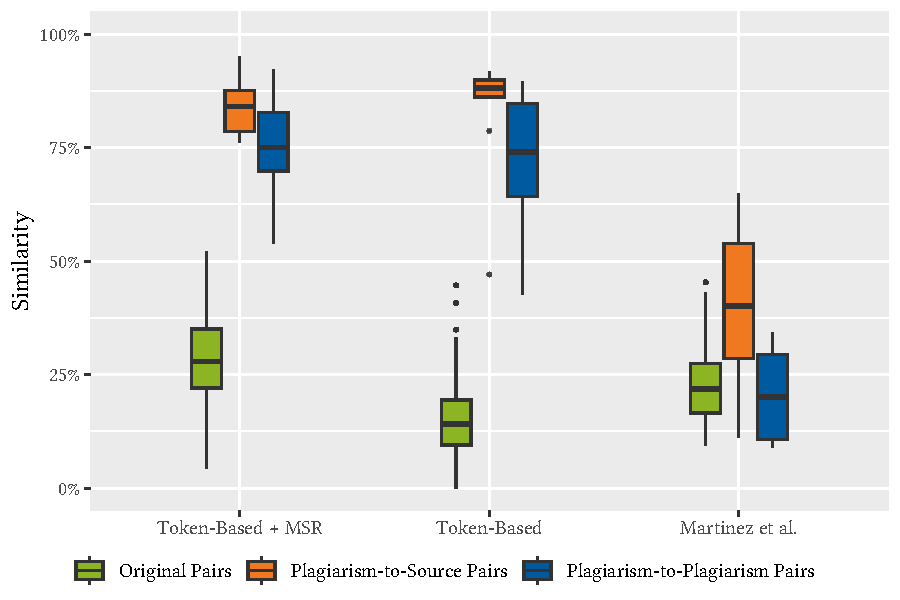
\includegraphics[width=1\linewidth]{figures/disseval2/experiment_avg.similarity.pdf}
\caption[Evaluation: Human Obfuscation of Models]{Results regarding human-generated plagiarism for our token-based approach (Token-Based) with and without MSR and the LSH-based approach by \citet{Martinez2020}.}
\label{fig:human-results}
\end{figure}

\noindent
The second stage evaluates based on instances of human-obfuscated plagiarism by novice modelers.
Note that these obfuscation attempts were the weakest in our overall evaluations. This motivates why automated obfuscation is a viable alternative for a potential adversary.

As discussed, we use our modeling plagiarism experiment dataset introduced in \autoref{sec:human-plagiarism} for this.
It consists of 31 metamodels, thus producing 210 unrelated, original pairs, ten plagiarism-to-source, and ten indirect plagiarism-to-plagiarism pairs (pairs of plagiarized models of the same source). Refer to \autoref{tab:student-obfuscation} for details on the employed obfuscation techniques.

\subsection{Results}
The results of the manually obfuscated plagiarism by novice modelers are illustrated in \autoref{fig:human-results}.
The results demonstrate that with MSR enabled, our approach can effectively distinguish the plagiarism-to-source pairs from the unrelated original pairs, as there is no overlap. Without MSR, our approach demonstrates good separation except for one outlier falling below 50 percent similarity. However, for the approach of \citet{Martinez2020}, the plagiarism-to-source pairs still exhibit increased similarities but overlap with the unrelated pairs, making detection more challenging.
When looking at the similarity differences in \autoref{tab:summary-stats-human}, we notice that the similarity differences are higher for our approach when MSR is disabled.
%
Similar results are observed for the plagiarism-to-plagiarism pairs. With MSR, our approach exhibits a clear separation between plagiarism pairs and unrelated pairs. Without it, there is sufficient separation between them, although a few outliers overlap with the unrelated pairs at around 40 percent similarity. In contrast, for \citet{Martinez2020}, the plagiarism-to-plagiarism median similarity falls below the median of the unrelated pairs, making detection next to impossible.
Again, when looking at the similarity differences, we notice that the similarity differences are higher for our approach when MSR is disabled.

\begin{table}%[h]
	\centering
	\begin{tabular}{llrrr}
		\toprule
		Plagiarism Type                             & Approach        & $\Delta$ Mean & $\Delta$ Median & $\Delta$ IQR  \\
		\midrule
		\multirow{3}{*}{Plagiarism-to-Source}       & Token-Based + MSR     & 55.47  & 55.40    & 43.79 \\
		                                            & Token-Based           & \B{69.19}  & \B{74.48}    & \B{65.57} \\
		                                            & Martinez et al. & 16.78  & 18.30    & 1.10 \\
        \midrule
		\multirow{3}{*}{Plagiarism-to-Plagiarism}   & Token-Based + MSR     & 46.36  & 46.55    & 33.25 \\
		                                            & Token-Based           & \B{57.03}  & \B{62.68}   & \B{43.74} \\
		                                              & Martinez et al. & -2.12  & -1.70    & -16.68 \\
		\bottomrule
	\end{tabular}
    \caption[Evaluation: Human Obfuscation of Models]{Similarity differences between the manually obfuscated plagiarism instances and the unrelated originals (higher means better detection) for the results in \autoref{fig:human-results}.}
	\label{tab:summary-stats-human}
\end{table}



\subsection{Discussion}
Some instances of manual plagiarism were sufficiently well-obfuscated to yield low similarities for our approach without MSR~\cite{Saglam2022}.
These instances accomplished this by heavily relying on reordering model elements, which is the vulnerability that MSR aims to address.
This observation aligns with the results of the first evaluation stage depicted in \autoref{fig:attacktypes-results}. MSR is explicitly designed to address this type of attack.
%
Nevertheless, both with and without MSR, our approach yields overall high similarities for plagiarism-to-source pairs.
We observed relatively weak obfuscation for these plagiarism pairs. The manual obfuscation observed here is thus weaker than automated obfuscation attacks.
Due to this weak obfuscation, MSR's effect is limited in many of the comparisons. However, it still notably improves the detection of outliers. 
We can observe a more noticeable impact of MSR for the plagiarism-to-plagiarism pairs, where the difference between the compared models is more pronounced, as it reflects the obfuscation efforts of two students instead of one.
%
Overall, our approach without MSR exhibits a lower similarity for the unrelated pairs, which can be attributed to our normalization technique.
The normalization reduces the impact of certain structural and syntactic variations between the unrelated pairs, thus slightly increasing their similarity.
This effect, however, does not impact the separability of the original from the plagiarism pairs.
In fact, the distinction between the stronger obfuscated instances and the original pairs is considerably more pronounced with MSR enabled than with it disabled.

\emph{In sum, our approach demonstrates strong performance in detecting human plagiarism, whereas the approach of \citet{Martinez2020} performs worse.}


% -------------------------
% Eval Stage 3
% -------------------------

\section{AI-based Obfuscation}\label{subsubsec:plaggpt}

\noindent
In our third and main evaluation stage, we evaluate the ability to detect comprehensively AI-obfuscated plagiarism.
%
As discussed in \autoref{subsec:chatgpt-obf}, we provided ChatGPT with models from the dataset and applied twelve different prompts for two metamodels to generate a total of 24 plagiarism instances. To evaluate the effects of even stronger obfuscation, we do not only evaluate with the plagiarism-to-source pairs but also with the pairs of plagiarized models of the same source (plagiarism-to-plagiarism, see \autoref{sec:metrics}).
Thus, we evaluate 24 Plagiarism-to-Source pairs and 132 Plagiarism-to-plagiarism pairs, which must be distinguished from the 210 unrelated original pairs (true negatives).

\subsection{Results}

\noindent
\autoref{fig:ai-obfuscated-models} shows the results for plagiarism generated by ChatGPT.
For the plagiarism-to-source pairs, our approach achieves high median scores of 78\% (MSR) and 74\% (no MSR), respectively. The approach of \citet{Martinez2020} has a significantly lower median score of 59\%. We observe similar results when looking at the difference between the plagiarism-to-source pairs and the unrelated original pairs as listed in \autoref{tab:summary-stats}. Our approach achieves the highest values for all three similarity \textit{difference} metrics ($\Delta$ Mean, $\Delta$ Median, and $\Delta$ IQR). Our approach without MSR follows closely by between three to five percentage points. The approach of \citet{Martinez2020} performs significantly worse, with 17 to 25 percentage points below our approach.

The differences between the approaches are even more prominent when looking at the similarity scores of the plagiarism-to-plagiarism pairs.
Our approach achieves a median score of 67\% with MSR enabled, 53\% without MSR, and \citet{Martinez2020} achieve only 43\%.
Our approach with MSR achieves the highest values for the difference between the plagiarism-to-plagiarism pairs and the unrelated original pairs listed in \autoref{tab:summary-stats}.
Without MSR, it achieves between eight to twelve percentage points less, \citet{Martinez2020} achieves between 21 to 25 percentage points less.

To determine the statistical significance of the evaluation results presented in \autoref{fig:ai-obfuscated-models}, we conducted one-sided Wilcoxon rank-sum tests with a significance level of $\alpha=0.05$. Ideally, to demonstrate a significantly improved performance, an approach has to show significantly higher scores for the plagiarism pairs (P2S and P2P) and significantly lower scores for the unrelated original pairs (OP). We both test for the effect of MSR and for the improvement of our approach with MSR compared to the approach of \citet{Martinez2020}. The results of the tests are summarized in Table \ref{tab:significance-stats}.
As the test statistic value ($W$) depends on the sample size and the sample sizes of the pair types differ, we use Cliff's delta ($\delta$) as a normalized metric for the effect size.

In the context of the Plagiarism-to-Source (P2S) and Plagiarism-to-Plagiarism (P2P) pairs, MSR significantly improved the similarity scores.
Furthermore, our approach performs significantly better than the approach of \citet{Martinez2020}.
While our approach with MSR achieves significantly lower scores for the original pairs (OP) compared to \citet{Martinez2020}, this is not the case for our approach without MSR.
However, the (negative) effect size of the original pairs is smaller than the effect sizes for the plagiarism pairs, which aligns with the similarity score differences in \autoref{tab:summary-stats}. As a consequence, this shift is negligible.
In summary, we observe both statistical and practical significance for the improvements brought by MSR and for the improvements of our approach (with MSR) compared to the one of \citet{Martinez2020}.

\begin{figure}
    \centering
    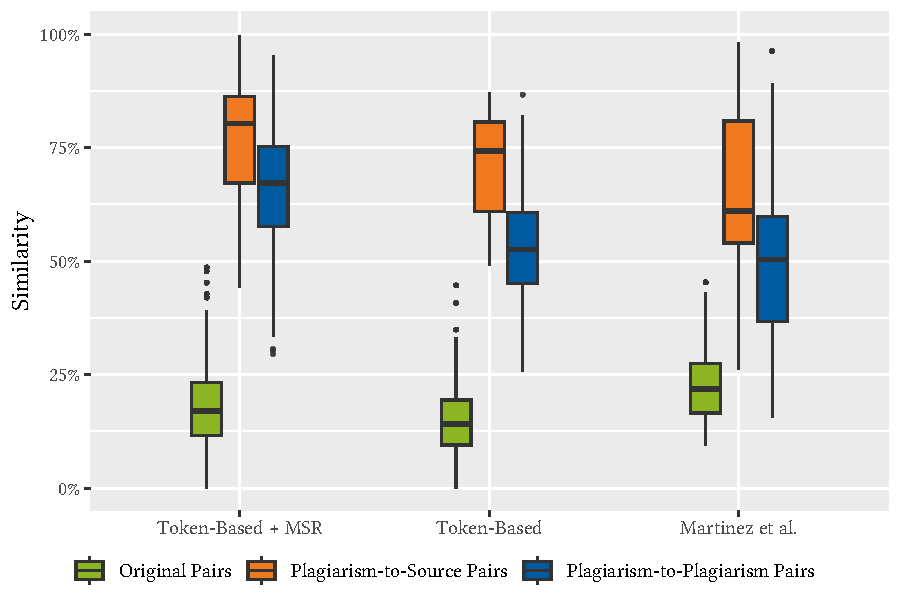
\includegraphics[width=\linewidth]{figures/disseval2/chatgpt_avg.similarity.pdf}
    \caption[Evaluation: AI-based Obfuscation of Models]{Results regarding ChatGPT-obfuscated plagiarism for our token-based approach (Token-Based) with and without MSR and the LSH-based approach by \citet{Martinez2020}.}
    \label{fig:ai-obfuscated-models}
\end{figure}

 \subsection{Discussion}
Our evaluation found that our approach significantly outperforms the state-of-the-art regarding the detection of AI-obfuscated models.
This is especially apparent when the obfuscation is strong, which is true for plagiarism-to-plagiarism pairs.
While our approach with MSR disabled also performs well, it is less resilient to strong obfuscation attempts.
This can be attributed to it being susceptible to reordering attacks, as shown in \autoref{subsec:first-stage}.
However, with MSR enabled, it is resilient to these attacks due to the benefits of this normalization technique.
Reordering and renaming are also likely the first steps a potential adversary would take after utilizing ChatGPT~\cite{Saglam2023}. 

The difference between our approach and \citet{Martinez2020} is even more considerable, as ChatGPT frequently employs renaming.
The renaming attacks of ChatGPT are particularly effective, as ChatGPT considers the modeling domain and identifies suitable synonyms.
Interestingly, as ChatGPT is partially deterministic, we observed recurring patterns for different prompts, such as inserting a \enquote{Node} and \enquote{Edge} class and adding references from specific existing classes to the inserted one. This shows that even with systematic prompt engineering and strong obfuscation, plagiarizers cannot be certain to avoid detection.

\emph{In sum, plagiarism generated with ChatGPT currently is predictable enough to be reliably detected by our approach. Our approach also significantly outperforms the state-of-the-art, especially for strongly obfuscated plagiarism.}

\begin{table}%[h]
	\centering
	\begin{tabular}{llrrr}
		\toprule
		Plagiarism Type                                             & Approach        & $\Delta$ Mean & $\Delta$ Median & $\Delta$ IQR  \\
		\midrule
		\multirow{3}{*}{Plagiarism-to-Source}                       & Token-Based + MSR            & \B{59.77}  & \B{64.39}    & \B{45.37} \\
		                                                            & Token-Based   & 56.87  & 60.22    & 40.23 \\
		                                                            & Martinez et al. & 42.16  & 39.27    & 26.54 \\
        \midrule
		\multirow{3}{*}{Plagiarism-to-Plagiarism}                   & Token-Based + MSR            & \B{48.01}  & \B{50.94}    & \B{33.80} \\
		                                                            & Token-Based   & 39.12  & 38.56   & 25.64 \\
		                                                            & Martinez et al. & 27.43  & 28.58    & 9.20 \\
		\bottomrule
	\end{tabular}
    \caption[Evaluation: AI-based Obfuscation of Models]{Similarity differences between the AI-based plagiarism instances and the unrelated originals (higher means better detection) for the results in \autoref{fig:ai-obfuscated-models}.}
	\label{tab:summary-stats}
\end{table}

\begin{table}%[h]
	\centering
	\begin{tabular}{lllrrrr}
		\toprule
		Comparison                                                  & Pairs & $H1$  & $p$         & $W$     & $\delta$ &   $n$  \\
		\midrule
		\multirow{3}{*}{Effects of Normalization}           & P2S & greater &  0.042  & 373     & 0.293         & 24         \\
		                                                              & P2P & greater & <0.001  & 13,024  & 0.495         & 132       \\
		                                                              & OP  & less    & 1.000   & 232,839 & 0.173         & 630    \\
		\midrule
		\multirow{3}{*}{{Token-Based + MSR to Martinez}}                  & P2S & greater & 0.008   & 405     & 0.406         & 24        \\
		                                                              & P2P & greater & <0.001  & 13,291  & 0.526         & 132        \\
		                                                              & OP  & less    & <0.001  & 131,810 & -0.336        & 630     \\
		\bottomrule
	\end{tabular}
    \caption[Significance: AI-based Obfuscation of Models]{Significance of the results in \autoref{fig:ai-obfuscated-models} assessed via one-sided Wilcoxon rank-sum tests (sign. level of $\alpha=0.05$, alternative hypothesis $H1$, p-value $p$, test statistic $W$, Cliff's delta $\delta$, sample size $n$) for Plagiarism-to-Source (P2S), Plagiarism-to-Plagiarism (P2P), and Original Pairs (OP).}
    \label{tab:significance-stats}
\end{table}

\section{Result Summary}\label{sec:mde-result-summary}
Our approach for token-based plagiarism detection for modeling assignments demonstrates broad resilience to algorithmic obfuscation attacks.
Notably, the approach of \citet{Martinez2020} shows vulnerability for renaming-based obfuscation, for which token-based approaches are inherently immune against.
For human-obfuscated plagiarism, our approach outperforms the approach of \citet{Martinez2020}, which encounters difficulties in detection.
Against AI-obfuscated plagiarism, our method achieves high similarity scores, especially in the strongly obfuscated plagiarism-to-plagiarism comparisons, thus outperforming \citet{Martinez2020} by a significant margin. The statistical tests further confirm the statistical and practical significance of these results.

Based on these results, we can answer the evaluation questions as follows:
\summaryBox{2.1}{Token-based detection approaches can successfully be applied to artifacts of modeling approaches, thus allowing for efficient and effective plagiarism detection.}
\summaryBox{2.2}{Token-based plagiarism detection significantly outperforms state-of-the-art modeling plagiarism detection when applied to modeling artifacts.}
\summaryBox{2.3}{Our token-based approach inherits the inherent immunity to renaming-based obfuscation but also achieves broad resilience against various human, algorithmic, and AI-based obfuscation attacks.}

In conclusion, we have achieved our evaluation goal \textbf{G2} of enabling token-based plagiarism detection for modeling assignments, providing a robust framework for identifying and addressing instances of plagiarism in this domain.

\section{Threats to Validity}
We now discuss how we address threats to the validity of our evaluation, following the guidelines outlined by \citet{Wohlin2012} and \citet{runeson2008}. These threats apply to the second goal of our evaluation, which aims to enable token-based plagiarism detection for artifacts of modeling assignments (\gref{2}).


\subsection{Internal Validity}
Internal validity refers to whether influences can unknowingly affect the analyzed variable concerning causality~\cite{Wohlin2012}.

    \textbf{Baseline Consistency:} For internal validity, we used the LSH-based approach of \citet{Martinez2020} as it is state-of-the-art. Besides this, we ensured that all other conditions remained constant when comparing the defense mechanism with each other or with the baseline. 

    \textbf{Baseline Parametrization:} As the approach of \citet{Martinez2020} is LSH-based, it provides several hyperparameters that may need to be adjusted to the modeling domain to maximize the detection rate. In detail, this involves the number of bands, which affects the strictness of the signature matching, and the number of rows per band, which controls the trade between precision and recall. This threatens internal validity, as incorrect or non-optimized parameter settings could affect the outcome~\cite{novak2018}. To mitigate this, we used the recommended parameters for \ac{EMF} metamodels discussed by the authors.

    \textbf{Human-Labeled Plagiarism}: If any datasets are manually labeled plagiarized, evaluator bias could influence these labels.
    However, this threat does not apply to our evaluation, as we can provide inherently correct labels for all plagiarism types.
    We generate the plagiarism instances for the automatic obfuscation, thus knowing which models are plagiarized.
    For human plagiarism, we obtained these by conducting a controlled experiment (see \autoref{sec:human-plagiarism}).

\subsection{External Validity}
External validity concerns the extent to which our findings can be generalized beyond the specific context of the evaluation. 

    \textbf{Availability of Datasets:} One potential limitation is the scarcity of publicly available modeling assignments datasets. Due to privacy and data protection policies, students' data is rarely published. For modeling plagiarism, we mitigated this by designing our evaluation around the widely used EMF-based metamodels, using a representative dataset from a real-world assignment~\cite{Saglam2023}.
    We thus transform it into three different data sets using various types of plagiarism (algorithmic, AI-based, and human).
    EMF-based metamodels are widely-used, and metamodeling is a typical assignment~\cite{Ciccozzi2018}.
    We acknowledge that additional datasets could provide further validation, yet the selected dataset and tasks reflect standard practices in educational settings.


    \textbf{Prompt Choice:} For AI-based obfuscation with ChatGPT, prompt choice is an essential factor influencing the strength and variability of AI-generated plagiarism. To control this, we conducted a pre-study in which we experimented with multiple prompts, incrementally adjusting them to increase the degree of obfuscation. By refining our prompts iteratively, we aimed to obtain representative results for AI-generated obfuscation effects while minimizing prompt variability as a confounding factor.

    \textbf{Generalizability of obfuscation attacks:}
    Limiting the evaluation to only a few types of obfuscation attacks could hinder the applicability of our results to broader contexts. To enhance external validity and thus ensure that our findings are generalizable, we included a diverse set of obfuscation techniques from the categories outlined in our threat model (see \autoref{sec:threatmodel-categorization}). Note that these are real-world obfuscation attacks that are, directly or conceptually, available in practice.

\subsection{Construct Validity}
Construct validity refers to how well the evaluation measures its intended purpose and whether the metrics and baselines chosen are appropriate. Thus, it relates to the degree to which we measure the theoretical construct we want to measure.

    \textbf{Evaluation Methodology Alignment:} To enhance construct validity, we aligned our evaluation methodology with those from established and related work. While we deviate from related works by not using a threshold-based classification, we do so to improve internal validity (see \autoref{sec:metrics}), as this method is fundamentally flawed. Finally, we employ an approach-independent ground truth, use established similarity metrics, and a Goal-Question-Metric plan~\cite{Basili1984, Basili1992}.

    \textbf{Underlying Research Object:} We ensure consistency between the research objects and the measurements via direct alignment. Since our study evaluates the effectiveness of modeling plagiarism detection, we use the similarity scores generated by the detectors as our primary measurement. Additionally, we directly utilize widely available techniques such as ChatGPT to assess automated obfuscation accurately.

    \textbf{Choice of Baseline:} The baseline selection might affect the comparison and outcomes. We addressed this by selecting the approach of \citet{Martinez2020} as the baseline, as it is, to our knowledge, the only other approach for plagiarism detection for modeling assignments.

\subsection{Reliability}
Reliability concerns the consistency of the results and whether the study can be replicated under the same conditions.


    \textbf{Replicability:} To ensure reliability, we provide a comprehensive replication package for our evaluation~\fancycite{replication-package}.

    \textbf{Use of Internal Datasets:} Using internal datasets can hinder reproducibility. Due to data sensitivity, only a partial dataset version is publicly available. We discussed any preprocessing steps and the employed obfuscation attacks for all datasets. Furthermore, we provide raw result data and metadata in our replication package. This enables researchers to replicate our experiments on other datasets, maintaining transparency and reliability.

%\todo{(LOW) Regarding \citet{Martinez2020}: Bad results for human plagiarism, however, may be a parameterization issue, as this approach relies heavily on that. We used the recommended parametrization for EMF metamodels, not further parameter tuning. For our approach, we also did no tuning and used default parameters.}


\part{Epilogue}
\chapter{Related Work}\label{cha:related-work}
In this chapter, we review research from multiple areas that intersect with the contributions of this dissertation.
We begin by discussing software plagiarism detection systems widely used in educational settings.
Second, we turn to research on clone detection, a problem that, while distinct from plagiarism detection, shares similarities in identifying structural similarities across codebases.
Third, we explore related work on obfuscation attacks and mitigation techniques related to our defense mechanisms.
Fourth, we address modeling plagiarism research in model-driven engineering, including model clone detection and model differencing.
Next, we discuss the similarities between plagiarism detection and automated assessment in computer science education.
Finally, we examine genome sequencing algorithms, a field whose techniques relate to one of our defense mechanisms.

% --------------------------------------------------------------------------------------------
\section{Software Plagiarism Detection Systems}
Plagiarism detection systems, often also referred to as plagiarism detectors, enable educators to tackle the problem of plagiarism at scale by helping to seek out plagiarism and deter it in the first place~\cite{Braumoeller2001}. 
Despite the early roots of software plagiarism and similarity research~\cite{Ottenstein1976}, \citet{Novak2019} observe that it is still an ongoing field of research, and the number of observed research studies has grown in recent years.
%
Most software plagiarism detection approaches compare the structure of the code~\cite{Nichols2019, Novak2019}; among them, token-based approaches are the most popular tools employed in practice.
\citet{Novak2019} criticize that despite the increased number of proposed tools and approaches in recent years, most remain inaccessible to the public, being used, if at all, exclusively by their creators and mentioned in only one article. They also note that many of these tools do not compare their work to others, raising concerns about their quality.

JPlag~\cite{prechelt2000} and MOSS~\cite{MOSS} are the most widely used tools \cite{Aniceto2021, Novak2019}.
Furthermore, JPlag is most frequently referenced and compared to \cite{Novak2019}. This is unsurprising, as JPlag is open source compared to MOSS and can be deployed locally. MOSS is closed-source; all student data must be sent to the MOSS server located in the United States. Thus, MOSS is not compatible with the \ac{GDPR} of the European Union. Finally, recently, MOSS enforced a strict rate limit of 100 submitted programs per day, which is insufficient for large courses.
Other tools mentioned frequently are Plaggie~\cite{Plaggie}, Sherlock~\cite{Joy1999}, and SIM~\cite{SIM}. However, they are partially outdated or no longer maintained.
One noteworthy modern tool is Dolos~\cite{Maertens2022}, which has been recently developed and conceptually borrows heavily from MOSS and JPlag.
Just like JPlag, it offers a modern user interface.
However, it is currently limited as it only supports single files and has limited language support.
All mentioned approaches are token-based and find matching fragments via hashing and tiling~\cite{prechelt2002, MOSS}. Specifically, JPlag~\cite{prechelt2000, prechelt2002} and Sherlock~\cite{Joy1999} use \textit{greedy string tiling} (with running Rabin-Karp matching as performance optimization)~\cite{Wise1993, Wise1995}, whereas MOSS and Dolos~\cite{Maertens2022} employ \textit{winnowing}~\cite{Schleimer2003}.

There are substantial differences between plagiarism detection systems for natural language and source code~\cite{Fincher2019, Simon2013, Simon2014b} as different techniques apply~\cite{Lancaster2005}. One key difference is that there are well-defined formal grammars for programming languages, and thus, the space of possible valid input programs is both more restricted and less ambiguous.
Thus, our work does \textit{not} relate to plagiarism detection for natural languages, written text, or similar textual artifacts. While many token-based software plagiarism detectors like JPlag have rudimentary support for (natural language) text, it is not recommended to rely on that as the current state-of-the-art in natural language processing employs completely different techniques like transformer-based models, which excel at capturing nuanced semantic relationships and meaning in the text~\cite{khurana2023, min2023}. These models go beyond simple token matching by understanding context and synonyms. This allows for the identification of paraphrasing and complex rewording~\cite{foltynek2019, manzoor2023}.

As our defense mechanisms are designed to extend state-of-the-art approaches and our modeling plagiarism detection approach applies token-based techniques for modeling artifacts, we consider token-based software plagiarism detection systems as the foundation for our work (see \autoref{sec:SPD}). Thus, we do not compare the different detection systems above in detail.
Our research, however, applies to any token-based software plagiarism detection system. We implement and evaluate our contributions with JPlag\footnote{Note that while it was developed at Karlsruhe Institute of Technology (KIT), it is also, based on the aforementioned factors, an ideal fit for our research contributions.} (see \autoref{sec:baselines}).

% --------------------------------------------------------------------------------------------
\section{Software Clone Detection}\label{sec:rw-clone-detection}
Reusing source code via copying is common in software development. This may involve minor adaptation, but a code fragment may evolve even if directly copied. Consequently, software systems often contain similar fragments called code clones~\cite{Roy2009}.
\citet{juergens2009} confirm that such code clones significantly impede modern software development.
Clone detection, denoting identifying such code bases, has been extensively researched \cite{Shobha2021review, ain2019, rattan2013, Roy2009}.
While both clone detection and plagiarism detection are software similarity problems~\cite{Novak2019}, they ultimately differ in many aspects~\cite{mariani2012}.
Clone detection usually seeks similar fragments in a single program, which is why plagiarism detection compares sets of programs.
Moreover, code clones are created accidentally~\cite{juergens2009}, while plagiarism is a deliberate act.

\citet{Hammad2022} present \textit{Clone-Seeker}, a tool designed for code clone search that leverages clone class metadata to improve the retrieval of syntactically and semantically similar code fragments. The metadata includes processed identifiers and a list of keywords capturing the semantics of the clone. This metadata allows developers to search for clones using queries.

\citet{wang2018} seek to specifically detect what they call \emph{large-gap} clones, meaning clones with big differences. Their tool \textit{CCAligner} tokenizes source code and finds fuzzy matches through a novel \emph{e-mismatch index}. Like many software plagiarism detectors, this approach is token-based. 
Thus, CCAligner works similarly to JPlag, though JPlag only considers exact matches. Of course, the main difference is that CCAligner aims to detect clones, whereas JPlag aims to detect plagiarism cases.

\citet{white2016} propose a deep learning approach for code clone detection by integrating both lexical and syntactic information. Their tool utilizes recurrent and recursive neural networks to learn representations for code fragments directly from software repositories, bypassing handcrafted features common in traditional methods. The approach captures similarities in a feature space that considers structural patterns and contextual usage by mapping terms to continuous vector spaces and employing a recursive structure over abstract syntax trees.
Like software plagiarism detectors, structural information is extracted from program syntax trees; the approach is ultimately based on deep learning. One disadvantage is, thus, that explainability and line-based traceability are limited, which is essential for plagiarism detection (see \autoref{sec:tsn-requirements}).

\citet{ly2017} aims to enhance clone detection through source code normalization using program dependence graphs. With this, they aim to find code clones altered more reliably via renaming, reordering, or statement insertion.
Their approach shares similarities with our token sequence normalization defense mechanism, as both use program dependence graphs for normalization. However, their approach normalizes source code, while ours normalizes token sequences. They consider code clones, and we consider plagiarism. Finally, our approach is language-agnostic.

\citet{li2024} present \textit{Prism}, a clone detection tool that uses behavior semantics extracted from assembly code to identify semantic clones. Prism generates representations by combining multiple instruction set architectures, specifically CISC and RISC, to capture nuanced memory and computational behaviors.
%
Compared to token-based plagiarism detectors, which focus on exact token matching and structural similarity, the reliance on assembly-level semantics provides resilience against structural variations. However, its dependence on specific instruction set architecture features might limit its robustness to obfuscation techniques that heavily alter assembly patterns. Furthermore, the approach is limited to specific languages because it relies on assembly code.

\citet{xu2024} introduce \textit{DSFM}, a functional clone detection tool that enhances detection by leveraging interactions between subtrees within abstract syntax trees. DSFM uses a recursive and recurrent network to encode subtrees, capturing both structural and semantic information, and applies a factorization machine to assess similarities at both program and block levels.
%
Unlike structure-based plagiarism detectors, it is designed to detect functional clones, meaning code snippets that perform similar functionality.

\citet{Dou2024} introduce \textit{CC2Vec}, a clone detection tool that combines token categorization with contrastive learning to enhance code clone detection, especially for semantic clones. CC2Vec encodes tokens into types and uses self-attention layers to produce vector representations, facilitating both syntactic and semantic detection. By applying contrastive learning, CC2Vec minimizes the effects of structural variations.
%
The complexity of setup and the need for specialized training make this approach less practical for straightforward plagiarism detection tasks.
Moreover, reliance on token categorization makes CC2Vec vulnerable to obfuscation techniques like variable renaming or structural changes, which can disrupt its token patterns. Unlike software plagiarism detectors, CC2Vec's complexity limits its adaptability against obfuscation.


Despite the similarities, however, plagiarism detection is a different field~\cite{mariani2012}, and clone detectors are insufficient for plagiarism detection.
In plagiarism detection, the goal is to accurately quantify the likelihood of code being plagiarized despite potential obfuscation attacks by an adversary.
In contrast, code clone detection does not consider scenarios where an adversary attempts to affect the process as code clones typically arise inadvertently~\cite{juergens2009}. As a consequence, clone detectors are vulnerable to obfuscation attacks.
Plagiarism detection approaches must deal with an additional layer of complexity introduced by the adversary-defender-scenario~\cite{Saglam2024b}.
Targeted obfuscation attacks thus make software plagiarism detection more challenging than clone detection~\cite{mariani2012}
Still, many clone detection approaches share similarities in their employed techniques~\cite{wang2018, ly2017, Dou2024, white2016}.
However, clone detection approaches currently seem to lean on machine learning techniques~\cite{feng2024}.

% --------------------------------------------------------------------------------------------
\section{Obfuscation Attacks and Their Mitigation}
Obfuscation attacks present a significant challenge for software plagiarism detection by obscuring similarities between plagiarized and original programs. While obfuscation has long been a concern~\cite {zhang2014b, Karnalim2016, Novak2019}, research on defending existing state-of-the-art plagiarism detection tools from obfuscation is limited. Most recent studies focus on developing entirely new approaches that often remain inaccessible to the public, as noted by \citet{Novak2019}. Research on mitigating obfuscation usually focuses on manual obfuscation and specific obfuscation types.
As automated obfuscation attacks are only discussed recently, research in that direction is even more sparse.
Among the few notable exceptions are the works of \citet{DevoreMcDonald2020}, \citet{Biderman2022} and \citet{zhang2014b}.

\citet{DevoreMcDonald2020} present \mossad, a tool that automatically generates undetectable plagiarized code variants, effectively defeating detectors like Moss and JPlag. By employing program transformation techniques inspired by genetic programming, \mossad generates multiple variants of a source code file that are semantically equivalent but evade detection (see \autoref{sec:foundations-mossad}). The non-deterministic nature of \mossad allows it to create diverse code variants that appear no more suspicious than authentic student submissions.

\citet{Biderman2022} examine how language models like \textit{GPT-J} can generate code that evades detection by Moss, a widely-used software plagiarism detection tool. Their study reveals that GPT-J can reliably produce correct, syntactically diverse solutions to introductory programming problems with minimal human intervention, avoiding Moss's similarity thresholds. This capability raises concerns for academic integrity as AI tools become increasingly accessible. Although Moss flags some fundamental transformations, it is ineffective against AI-generated code, which introduces unique structural patterns undetectable by current plagiarism methods.

\citet{Foltynek2020} address the challenge of detecting machine-obfuscated plagiarism, explicitly focusing on text rewritten by online paraphrasing tools. Their approach evaluates various word embedding models combined with classifiers, thus distinguishing human-written from machine-paraphrased text.
%
While this is one of the few works focusing on \textit{automated} obfuscation, it covers plagiarism of natural language, not source code. Thus, it is not applicable to the challenges we discuss in this dissertation. Our contributions only consider software plagiarism.

% --------------------------------------------------------------------------------------------
\subsection{Resilience via Code Normalization}
%Code normalization is also utilized in various other research areas.
Code normalization simplifies code by reducing syntactic variability, making it easier to identify bugs, enforce coding standards, and detect duplicates. It is used in areas like bug detection, automated code review, clone detection, and machine learning on source code.
%
While the previously discussed research of clone detection approach of \citet{ly2017} comes closest to our defense mechanism of token sequence normalization (see \autoref{sec:rw-clone-detection}), code normalization is used in many research areas.

%While Ly's normalization comes closest to our approach, normalization is a standard pattern in code comparison. 
In general, we can distinguish between two types of normalization: \emph{lexical normalization} and \emph{structural normalization}.
%
\emph{Lexical normalization} provides invariance to lexical modifications. Program semantics need not be considered. \citet{roy2008} employ lexical normalization to detect code clones, specifically aiming to disregard superficial editing differences to allow textual line-by-line code comparison. They introduce a parser-based, lightweight approach called \textit{NICAD} that leverages a source transformation system to detect near-miss clones by simplifying and normalizing C code accurately. %; they rename all identifiers to @id@, for example.
\citet{allyson2019} seek to improve a text-based plagiarism detector. They do this with several preprocessing techniques, such as removing whitespace.
The tokenization step of token-based detectors abstracts from specific details like whitespace, names, and types; it is a form of lexical normalization. Thus, our defense mechanism does not need to consider lexical modifications as immunity to them is inherently given, markedly differentiating it from the works above.

Our defense mechanism token sequence normalization is a form of \emph{structural normalization}. This type of normalization makes code comparisons invariant to structural modifications. Program semantics must be considered here, making structural normalization more complex than lexical normalization. It may be more accurate to view structural normalization as a type of program analysis rather than code normalization, as code in its textual form is usually not directly considered. Instead, programs are parsed and then further processed or analyzed.

\citet{wang2008} use structural normalization to simplify program analysis by bringing code into a consistent form. They use the system dependence graph, a generalization of the PDG. 
%
They construct the graph directly from the source code and consider it the result of the normalization.
This presents the first difference to token sequence normalization. Another difference is, once again, that we do not construct our graph directly from the source code. In contrast to their approach, we specifically focus on identifying instances of plagiarism.

\citet{Schott2024} present \textit{jNorm}, which performs bytecode normalization to facilitate code similarity detection across Java applications compiled with different environments. By transforming Java bytecode into a stable intermediate form, jNorm addresses differences caused by varying compilers, Java versions, and target levels, which often obscure similarity analysis.
%
Their approach can align bytecode for consistent comparison in plagiarism detection. However, unlike general plagiarism detectors, jNorm is specifically tailored to Java programs.

Besides detecting plagiarism and clones, program comparison is also used to detect malware. Like plagiarism detection in a business context, malware detection must work with bytecode, as source code is usually unavailable. \citet{bruschi2007} use structural normalization for malware detection. They consider their normalization a form of optimization. They apply several normalizing transformations to programs, such as dead code removal. From the resulting normalized programs, they construct graphs. Like previously mentioned approaches, they compare graphs directly, which serves to differentiate token sequence normalization. Once more, token sequence normalization is also different because we do not work with bytecode.

In summary, our work distinguishes itself from previously mentioned normalization approaches by being language-agnostic and specifically addressing obfuscation techniques used to disguise plagiarism.

% --------------------------------------------------------------------------------------------
\subsection{Resilience via Graphs}
There are some graph-based approaches to plagiarism detection~\cite{Novak2019}, for example, based on program dependence graphs~\cite{ferrante1987}. While graph-based approaches may be potentially less vulnerable to some obfuscation attacks, they are not feasible in practice~\cite{liu2006} due to the NP nature of subgraph isomorphism~\cite{Shang2008, McCreesh2020, Lubiw1981}.

Graph-based approaches, such as \textit{GPlag} by \citet{liu2006}, compare graphs directly instead of linearizing the program. Thus, they use a more detailed program representation. This can be leveraged to achieve resilience against \textit{some} obfuscation attacks like dead code insertion.
Determining subgraph isomorphism NP-complete and doing so pairwise for many programs does not scale well and makes these approaches impractical.

Program behavior is resilient to semantic-preserving obfuscation attacks and, thus, can also be used for plagiarism detection.
\citet{cheers2021} present the plagiarism detector BPlag. It uses symbolic execution to extract behavior from source code and calculates a similarity score by comparing graphs representing the extracted behavior.
As symbolic execution and graph comparisons are both computationally expensive, the runtime of BPlag is too high for practical use, much like GPlag. Along with their implementation of BPlag, the authors provide a notice acknowledging this: "\textit{BPlag is computationally complex, requires lots of RAM and disk space, and does not scale to large data set sizes. It should not be used on conventional computers - HPC workstations only.}"~\cite{bplag-github}

\citet{chae2013} aim to detect plagiarism on a bytecode level by comparing the sequence and frequency of API calls. They do so with a novel graph called API-labeled control flow graph (A-CFG), which captures both the sequence and frequency of API calls to reflect the functionality of a program. They then apply a random walk with restart (RWR) to compute a score vector for each graph, allowing scalable similarity comparisons through vector cosine similarity rather than direct, costly graph matching.
%
Our defense mechanism token sequence normalization similarly builds a graph representation and reduces it for efficient comparison; however, while they focus on bytecode and API call patterns, our work applies to any programming language and focuses on structural similarity. Approaches based on vector similarity do not provide sufficient traceability and explainability (see \autoref{sec:tsn-requirements}).


\citet{zhang2014} propose \emph{LoPD}, a plagiarism detection system that shifts focus from detecting similarities to identifying dissimilarities in program behavior. LoPD uses symbolic execution and weakest precondition reasoning to analyze computation paths, aiming to find inputs that lead two programs to produce different outputs or execute semantically different paths. If LoPD finds any such dissimilarity, the programs are deemed distinct; otherwise, it suggests potential plagiarism. This method enhances resilience against obfuscation techniques, basing its comparison on formal program semantics.
However, its reliance on symbolic execution and constraint solving means LoPD can be computationally intensive and less effective for small programs with simple logic, as these may produce false positives due to coincidental path alignment. Moreover, their approach is limited to C and C++ programs.

These graph-based approaches thus relate to our defense mechanism token sequence normalization, which also leverages the advantages of graph-based approaches via program dependence graphs. However, our defense mechanism operates on a token level rather than a source code level. This means we construct the program dependence graph based on tokens, and the approach is thus language agnostic. Finally, via token sequence normalization, we normalize the internal representation of each input program, but we do not conduct a graph-based comparison. Thus, we preserve the scalability of token-based approaches and combine the best of both worlds.

% --------------------------------------------------------------------------------------------
\subsection{Resilience via Intermediate Representation}
\citet{DevoreMcDonald2020} propose using semantic checking of intermediate representation (assembly and Java byte code) to defend against \mossad, their automated, threshold-based, insertion-based obfuscation attack. However, this language-dependent defense mechanism is conceptual and is yet to be realized.
We also explored this idea by using the LLVM-IR code for plagiarism detection \cite{Heneka2023}. The usability and platform dependence of LLVM limits this approach.

\citet{Karnalim2016} propose a bytecode-based approach for detecting source code plagiarism in introductory Java programming assignments. Unlike source code approaches that rely on language-specific features, this approach operates on Java bytecode, which remains stable and removes syntactic sugar. Essential techniques include instruction generalization, reinterpretation, and method linearization to handle common plagiarism tactics. Thus, the approach is resilient to superficial code modifications often seen in student assignments.
This approach, however, is Java-specific and thus does not support non-JVM languages. Furthermore, it requires the program to compile into byte code. Finally, their predefined criteria limit the proposed preprocessing strategies; adversaries may bypass detection via obfuscation attacks that fall outside the filtered scope.
%
In contrast, our defense mechanisms are language-independent or language-agnostic and less limited in relating to programming correctness. In fact, subsequence match merging works even for syntactically incorrect programs as long as the detector can create tokens for them.

\citet{Luo2017} present \textit{CoP}, a binary code similarity comparison tool that is resilient to code obfuscation. CoP uses symbolic execution and longest common subsequence (LCS) analysis on semantically equivalent basic blocks to identify similar code segments in binaries, regardless of transformations or compilation differences. By comparing symbolic representations at the basic block, path, and program levels, CoP achieves high robustness against obfuscation techniques, such as control flow flattening and dead code injection. Due to its restriction to binary code, their approach is limited to C and C++ programs.
Furthermore, their approach is resource intensity due to symbolic execution and LCS-based analysis, which makes it computationally expensive and less practical for large codebases.

In summary, approaches based on intermediate representation, such as assembly or byte code, provide obfuscation resilience.
However, these methods have several drawbacks, such as being language-dependent, requiring significant computational resources, and lacking traceability and explainability.
However, they come with several limitations, like language dependence, high computational cost, and a lack of traceability and explainability. In contrast, our defense mechanisms do not suffer from these limitations and provide strong resilience.

% --------------------------------------------------------------------------------------------
\subsection{Resilience via Preprocessing}

\citet{Novak2020} examines the challenge of detecting source-code plagiarism in academic settings, focusing on preprocessing techniques to enhance the accuracy of plagiarism detection tools.
This involves, among other aspects, the resilience against obfuscation.
One notable approach, common code deletion, involves removing frequently reused code elements from student submissions before entering the detection pipeline. They categorize certain code elements, such as template-based structures, as common code, as they do not contribute to detecting plagiarism meaningfully and may even serve as obfuscating insertions. 
As an example, this involves getters, setters, and empty methods.
By excluding such elements in advance, plagiarism detectors gain inherent resilience against specific types of semantic-preserving obfuscation attacks. However, this approach is limited to predefined common code types; an adversary could bypass it by inserting different, unrecognized elements, thus limiting the robustness of this defense.
Moreover, they emphasize the need for calibration and comparative analysis across tools to understand how preprocessing techniques contribute to the effectiveness of plagiarism detection.

Similarly, \citet{Karnalim2020} investigate the impact of various preprocessing techniques on the accuracy and efficiency of source code similarity detection in introductory programming courses. They examine 16 preprocessing techniques, such as comment and identifier removal, syntax tree linearization, and renaming, assessing how each affects similarity comparison. Their findings suggest that steps like identifier removal improve both efficiency and effectiveness, while others, like syntax tree linearization, enhance accuracy at the expense of speed. These insights are valuable for designing detection tools and helping educators understand potential disguises students might apply to copied code.
While these preprocessing techniques are effective, they cannot provide broad obfuscation resilience.
For example, these techniques do not address the threat of obfuscation based on statement insertion.

\citet{cabre2014} studies how using code obfuscators like \textit{ARTIFICE} and \textit{ProGuard} affects different plagiarism and clone detection systems. Out of all tools, JPlag performs third best. They propose using deobfuscation tools, which improve the resilience of detection systems across the board. This defense mechanism, however, is very attack-specific. Furthermore, it is a preprocessing technique that must be done for each input program.

% Final words:
\noindent
In contrast to all aforementioned approaches, our defense mechanisms are either language-independent or language-agnostic. Subsequence match merging is also attack-independent. Our defense mechanisms also operate on the abstract level of the matched subsequences, thus improving generalizability. In contrast to the mentioned approaches, our defense mechanisms provide broad resilience against automated obfuscation attacks.
However, even more importantly, this ensures that our approaches do not modify the source code of the input programs. This is crucial, as gathering and presenting evidence must be possible for the original, unaltered programs (see \autoref{sec:tsn-requirements}).

% --------------------------------------------------------------------------------------------
\section{Plagiarism in Modeling Assignments}

\noindent
This section reviews research related to modeling plagiarism and its detection.
Note that there are next to no other approaches for modeling plagiarism detection~\cite{Martinez2020}.
We thus also discuss approaches from model clone detection and model differencing, which are unsuitable for plagiarism detection due to their vulnerability to obfuscation attacks~\cite{Saglam2022} and computational inefficiency for large courses~\cite{Martinez2020}.

% --------------------------------------------------------------------------------------------
\subsection{Modeling Plagiarism Detection}
\citet{Martinez2020} utilize \emph{Locality Sensitive Hashing} (LSH), an approximate nearest neighbor search mechanism, to detect plagiarism. They embed models into a similarity metric space by transforming them into context-aware fragments that are turned into integer vectors using \textit{minhash} on the names of the fragment's classes, attributes, and operations.
The model signatures are then computed using LSH, and the similarity of any two models is determined by the hamming distance between the two signatures. 
Unlike ours, theirs combines contextual rather than structural information, rendering it vulnerable to obfuscation attacks.
To our knowledge, the LSH-based performs well and is the only other approach for modeling plagiarism detection.

However, it has some limitations.
The LSH signatures are computed based on names, so their approach is prone to renaming-based obfuscation attacks.
Furthermore, their approach is not resilient against attacks based on randomly inserting features like attributes and operations \cite{Saglam2022}.
These are common obfuscation attack types~\cite{Saglam2023, Novak2019}.
In contrast, our approach is resilient against these attacks.
Moreover, their approach does not provide sufficient information on how similarities are calculated, hindering traceability and explainability and making manual inspection significantly harder. 
In contrast, our approach provides detailed information on how the different elements contribute to the similarity score.

\citet{cornic2008} presents a plagiarism detection tool for source code, however, built on the Eclipse Platform using a model-driven approach. This allows the tool to analyze source code from multiple programming languages by converting it into instances of a high-level language-independent metamodel consisting of statements, blocks, classes, functions, calls, and control structures. They generate Java code for each model instance via EMF, enabling the comparison across different languages.
The tool involves multiple components: a generic front-end for model conversion, a back-end comparison engine, and a results display interface.
%
Besides the fact that this approach uses a generic metamodel for programming languages and model transformation to parse code and generate a Java representation, the approach compares programs similar to other token-based approaches via greedy string tiling~\cite{Wise1993}. Thus, this approach uses model-driven techniques for source code plagiarism detection but does not support modeling plagiarism detection. In contrast, our approach enables modeling plagiarism detection, thus allowing token-based plagiarism detectors to support both models and code.

% --------------------------------------------------------------------------------------------
\subsection{Model Clone Detection}

\noindent
Model clone detection~\cite{Shobha2021, Hammad2022} deals with finding syntactically or semantically identical model fragments in a larger model or across multiple models.
While the employed techniques are similar to modeling plagiarism detection, modeling clone detectors are not designed to withstand the threat of obfuscation attacks. Thus, they are essentially different tasks.
%
For model clone detection, the extent of a modification should be reflected in the similarity measures for a given model fragment.
In contrast, some changes should not reduce the similarity for plagiarism detection. This allows for resilience against obfuscation attacks.

\citet{Deissenboeck2008} present a graph-based approach to detect clones in model-based development, specifically for large Simulink models used in automotive control systems. The method normalizes model structures, applies graph algorithms to find clone pairs, and clusters them for further analysis. Their approach shows the potential to improve maintenance by identifying reusable components and reducing redundant code in model-based systems.

\citet{Stoerrle2013} address the challenge of detecting model clones in UML domain models, drawing parallels between clone issues in code-based and model-based development. They introduce a tool that applies various algorithms and heuristics to identify UML model clones, highlighting that existing techniques for code clone detection are not directly applicable to models due to unique structural and semantic differences. They discuss that each detection approach has limitations, indicating a need for further refinement.
%
Based on this work, \citet{Stoerrle2015} propose an improved clone detection approach for UML domain models. This approach is notable for its broad applicability across various UML model types and its ability to detect clones with high accuracy and speed. 

\citet{Strueber2016} investigate clone detection in graph-based model transformation languages. They present a customized approach for identifying clones in transformation rules to detect structural patterns in graph-based languages. The study outlines specific requirements for clone detection in \ac{MDE} through use cases such as clone refactoring and performance improvement.

\citet{Babur2019} present \textit{SAMOS}, a framework for detecting metamodel clones in large repositories, focusing on EMF metamodels. SAMOS uses natural language processing, vector space modeling, and clustering to detect similar model fragments. They evaluate SAMOS against tools like NICAD-Ecore and MACH, showing that SAMOS achieves high accuracy and scalability for clones across multiple datasets. While their approach performs well for clone detection, it is prone to obfuscation attacks based on renaming, retyping, and attribute value changes. Thus, it is not sufficient for metamodel plagiarism detection.

% --------------------------------------------------------------------------------------------
\subsection{Model Differencing}
\noindent
Model Differencing is extensively researched \cite{Kessentini2014, Stephan2013} and is commonly used for model versioning, which involves comparing different states of the same model.
Various model differencing approaches exist~\cite{Kolovos2009, Zadahmad2019, Maoz2011}.
They are loosely related to plagiarism detection systems, as both determine model similarity.
Nevertheless, model differencing approaches are not designed for a scenario where an adversary intentionally obfuscates similarity. Thus, they are vulnerable to fundamental obfuscation attacks.

One of the early approaches is \emph{UMLDiff}~\cite{Xing2005}, which provides model differencing based on custom similarity metrics. Since these metrics are specifically designed and optimized for UML models, their application is limited to the UML domain.
\emph{DSMDiff} proposed a similar approach which rather supports arbitrary metamodels \cite{lin2007}.
%
Metamodel-agnostic model differencing suffers from reduced accuracy due to the task's inherent complexity, which has been shown for EMF Compare and DSMDiff by \citet{Kolovos2009}. \citet{Pietsch2013} present a set of model evolution scenarios that often pose problems for model differencing approaches.

The most widely used metamodel-independent approach and thus the de-facto standard is \emph{EMF Compare}~\cite{Brun2008}.
It uses similarity metrics for model matching and provides a high degree of customizability, thus allowing the design of custom matching strategies. As EMF Compare itself is model-driven, the derived changes are represented by a metamodel, enabling further use of model transformations.
EMF Compare's identifier-based strategy fails to detect plagiarism, as changing identifiers is an easy obfuscation attack.
%
Furthermore, its similarity-based strategy is susceptible to renaming and reordering-based attacks.
We demonstrated this in a different context~\cite{Wittler2023}, yet the same principles hold true for obfuscation attacks.
Since EMF Compare allows custom strategies, our approach for modeling plagiarism detection could be implemented as such a strategy in order to use the visualization EMF Compare provides. However, we could also employ related approaches for change visualization~\cite{Brand2010, Brand2010b}.

In contrast to the syntactic approaches like EMF Compare, which compares the concrete or abstract syntax of models, semantic model differencing compares models in terms of their meaning by leveraging semantic matching \cite{Maoz2011, Maoz2016}. Multiple approaches for semantic model differencing have been proposed \cite{Langer2014, addazi2016}.
\citet{Maoz2016} provide a framework to relate syntactic and semantic model differences.
However, just as syntactic approaches, they are not intended for plagiarism detection and thus offer no resilience to obfuscation attempts.

% --------------------------------------------------------------------------------------------
\subsection{Image Plagiarism Detection}
Our work primarily focuses on modeling artifacts in the MDE domain. This involves specifically domain models and their digital artifacts and does not include images or image-based diagrams.
We thus only loosely relate image-based plagiarism detection, which focuses on identifying similarities in visual content such as images or diagrams~\cite{Ovhal2015, hurtik2015, meuschke2018}. In contrast, modeling plagiarism detection involves comparing structured data representations, like UML models, requiring specialized techniques assessing the semantic and structural similarity between model elements rather than visual features.
Moreover, like natural language processing, state-of-the-art image recognition uses completely different techniques~\cite{li2022, Shafiq2022}.

\citet{umam2021} evaluate the effectiveness of the Perceptual Hash algorithm in detecting similarity in UML sequence diagram images, even when subjected to rotations and skewing. Their findings indicate that these common disturbances do not significantly affect the ability of the algorithm to detect plagiarism, maintaining a similarity detection rate above 60 percent.

\citet{dahanayake2021} propose an approach to detect plagiarism in enhanced entity-relationship (EER) diagram images using deep neural networks, image processing, OCR, and text similarity algorithms. This approach provides accurate, fast plagiarism detection, generating a similarity report to aid in examination marking and discourage academic misconduct in diagram-based assignments.

\citet{skuruvila2017} present a flowchart plagiarism detection system based on image processing that compares shapes, orientation, and text by converting flowcharts into graphs. This graph-based approach detects plagiarism even with rearranged flowchart elements, demonstrating accuracy across different shapes and orientations.

\citet{parmar2024} introduce \textit{VIBRANT-WALK}, an algorithm for detecting image plagiarism of figures in academic papers by comparing images to a repository of published content. The two-stage process uses a \textit{vibrancy matrix} for contour detection and a pixel-by-pixel comparison through random walks, achieving high accuracy on a custom dataset of research article images.

All approaches mentioned above focus on image-based plagiarism detection. Furthermore, these approaches focus on a single type of diagram, for example, sequence diagrams or flowcharts. Thus, they are not applicable for modeling plagiarism detection.

% --------------------------------------------------------------------------------------------
\section{Automated Assessment in Computer Science Education}
Plagiarism detection also relates to automated assessment in computer science~\cite{mala-mutka2005}, which refers to using software tools and systems to evaluate students' programs without requiring manual grading.
Automated assessment is essential in programming courses because it provides immediate, consistent feedback and scales large courses, where the submitted solutions for one assignment can total hundreds of thousands of lines of code.
Automated assessment for programming assignments is a widely researched field~\cite{Messer2024, paiva2022, higgins2005, mala-mutka2005}.
%
\citet{zschaler2018} explore the importance of modularity in automated assessment systems, especially in the context of scaling and flexibility in programming education.
They introduce their \textit{NEXUS} platform, which allows for independent execution and scaling of components, enabling flexibility for educators to tailor grading processes.

Our approach to modeling plagiarism detection is loosely related to automated assessment for modeling assignments, which educators recognize as a crucial requirement~\cite{Kienzle2024}. One example is the automated grading of UML models~\cite{Bian2019, Bian2020, Boubekeur2020, Hasker2011}.

\citet{Hasker2011} introduces \textit{UMLGrader}, an automated tool that provides feedback on student-created UML class diagrams by comparing them against a reference solution. UMLGrader identifies missing or incorrect elements, such as class names, associations, and multiplicities. Their evaluation shows that it improves the accuracy of students in constructing diagrams, especially for constrained problems with a clear expected solution, making it beneficial for teaching foundational UML concepts.

\citet{Bian2019} propose an automated grading approach for UML class diagrams, addressing the challenge of manually grading large volumes of assignments with varied, correct solutions. Their approach uses a metamodel to map instructor solutions to student submissions and an algorithm that applies syntactic, semantic, and structural matching to assess alignment with the solution template. By assigning partial marks for minor errors, such as misplaced attributes or associations, their tool, implemented in the \textit{TouchCORE} platform~\cite{schottle2015}, achieves a grading accuracy close to human assessments.
%
Moreover, \citet{Bian2020} investigate the effectiveness of automated grading for UML class diagrams through case studies in introductory and advanced software engineering courses. The study highlights the need for flexible grading criteria, as instructors may have different grading styles, and multiple correct solutions often exist for modeling problems. They address this by incorporating configurable grading settings and alternative solution models.

\citet{hosseinibaghdadabadi2023} introduce an automated grading system for use case models. The proposed system uses structural, syntactic, and semantic matching techniques and natural language processing to align student use cases with instructor models. A flattening algorithm removes hierarchical structures, simplifying comparison by directly matching individual use case steps. The flattening step bears similarity with the tokenization step in token-based plagiarism detection, where models or programs are linearized.

\citet{chen2024} propose an embedding-based approach for automated assessment of domain models. The system leverages text embeddings and graph similarity techniques to match student-generated domain models with instructor-defined reference models automatically. The approach involves multi-stage matching of classes, attributes, and relationships within the models, using cosine similarity and graph edit distance for accuracy.
%
Their approach shares similarities with token-based plagiarism detection systems like JPlag in its use of similarity scoring and structural matching of elements. However, it relies on element identifiers for matching, which is not suited for modeling plagiarism detection due to the threat of obfuscation attacks.

\citet{hamann2024} introduce a model-driven approach to address interoperability challenges in automated assessment systems for computer science education. To that end, they provide a technology-independent assessment model, allowing assessment content to be transformed for various systems. This three-stage approach involves creating a meta-assessment model, generating task-specific assessment rules, and producing technology-specific representations. The system facilitates automatic, semi-automatic, and manual assessments while enabling flexibility and reusability in instructional resources.

We identify three key aspects that define the differences between automated assessment and plagiarism detection systems in computer science education. Automated assessment aims to detect and evaluate differences between student submissions and a solution, measuring correctness. By contrast, plagiarism detection prioritizes identifying similarities despite the potential for obfuscation, meaning it must be robust against intentional alterations designed to obscure plagiarized content.
%
Additionally, plagiarism detection operates in an adversarial context, where students may attempt to evade detection by disguising similarities through various obfuscation techniques. Automated assessment, however, sees the opposite behavior: students aim to align their submissions as closely as possible with the solution, focusing on correctness rather than concealment.
%
Scalability also differs significantly between these processes. Automated assessment generally involves a linear complexity, where the work of each student is compared to either a single solution or a small set of solutions. This results in a linear comparison process with a $O(n)$ complexity. In contrast, plagiarism detection typically requires pairwise comparisons among all submissions, resulting in $O(n^2)$ complexity, making efficient performance optimization more critical for practical application in large courses.

% --------------------------------------------------------------------------------------------
\section{Genome Sequencing}\label{sec:rw-genome} % in Bioinformatics}
We also relate to research related to genome sequencing in bioinformatics, which is the process of determining the entire genetic sequence of a specific organism or cell type.
%
In bioinformatics, \textit{Indel} detection is used to identify pairs of genome sequences that differ due to insertions and deletions (indels). This sequence variation is essential for studying genetic mutations and understanding human diseases. Interestingly, the core challenge in indel detection is conceptually similar to software plagiarism detection, where identifying similar program pairs despite minor alterations in token sequences is crucial. Both tasks fundamentally detect meaningful sequence alignment amid small, possibly superficial changes.

\textit{TransIndel}, developed by \citet{Yang2018}, is a framework designed specifically for detecting indels by comparing genome sequences composed of specific sequence segments called \textit{chimeric reads}. TransIndel operates by taking two sequences as input and iterating through them using a fixed window size to analyze chimeric reads. 
It then evaluates possible alignments within this window to infer insertions or deletions. When two possible alignments occur due to an extra chimeric read in the target sequence, the framework marks the chimeric read as deleted from the read sequence. Conversely, if no alignment is possible because of an additional read in the read sequence, it is marked as inserted into that sequence. TransIndel effectively aligns sequences while remaining robust to indels by focusing on possible alignments with this iterative window.

The fixed window algorithm has some similarities to greedy string tiling~\cite{Wise1993} and winnowing~\cite {Schleimer2003}. In fact, greedy string tiling has seen use in bioinformatics~\cite{Wise1995}, particularly for aligning nucleotide or amino acid biosequences. This approach can detect transpositions, rearrangements, and repeated substrings that are often missed by earlier alignment algorithms, such as those based on dynamic programming.
Additionally, the ability of the algorithm to group amino acids based on substitution matrices enhances its biological relevance, allowing it to account for evolutionary mutations. Greedy string tiling was thus particularly used for large-scale sequence comparisons and database searches.

Moreover, the fixed window algorithm is similar to one of our defense mechanisms.
The principles of insertion and deletion in sequence alignment closely resemble the ideas of subsequence match merging, which heuristically merges split matches to reverse the effects of obfuscation attacks. A difference, however, is that subsequence match merging operates heuristically in order to avoid assumptions on the underlying token sequence and the presence of obfuscation, thus making it attack-type independent. In contrast, the fixed window algorithm involves string domain-specific considerations regarding genome sequences. Furthermore, subsequence match merging works iteratively and terminals when no more matches can be merged. In contrast, the fixed window algorithm does not iterate repeatedly but only processes sequences sequentially in a single pass.

The \textit{Needleman–Wunsch algorithm}~\cite{Needleman1970} uses dynamic programming to find the globally optimal alignment between two sequences. In Bioinformatics, genome sequences are aligned by applying a scoring system where matches, mismatches, and gaps (often representing indels) are assigned specific points. The algorithm builds a matrix to compute the best alignment score between two sequences, with the final score located in the bottom-right cell. By backtracking through this matrix, the algorithm identifies the optimal alignment path.

Although computationally intensive, this approach could theoretically be applied to software plagiarism detection, aligning token sequences with an appropriate scoring system to assess similarity. However, the high computational complexity of the algorithm may make it impractical for larger datasets or courses with extensive code submissions.
%
Conversely, subsequence match merging \textit{could} be applied for problems in bioinformatics.
However, it does not compute an alignment path or seek an optimal global alignment (e.g., to maximize the sequence similarity).

\chapter{Future Work}\label{cha:future-work}
While this dissertation provides advancements in detecting software plagiarism and resilience against obfuscation attacks, it also opens up new avenues for further exploration. The following discusses possible future work, emphasizing how our contributions can be extended, complemented, or applied to new problems.

We begin by summarizing the limitations of our contributions and discussing future work that arises from them.
Second, we discuss future work on cross-language and multi-language plagiarism detection.
Next, we discuss emerging threats, especially with a focus on generative AI.
Finally, we will discuss how our contributions could be applied in other fields, such as clone detection, automated assessment, and even bioinformatics.


\section{Addressing Current Limitations}

For each of our contributions, we detailed their current limitations in \autoref{sec:tsn-limits}, \autoref{sec:smm-limits}, \autoref{sec:msr-limits}, and \autoref{sec:mde-limits}.
In the following, we discuss related work motivated by these limitations, showing what aspects could be improved upon in the future.

\begin{description}
\item[Token Sequence Normalization]
As discussed in \autoref{sec:tsn-limits}, token sequence normalization is highly effective against insertion-based obfuscation attacks but has two limitations. The first limitation is that its effectiveness depends on the quality and accuracy of the extracted language-specific semantic information. In our evaluation, we discussed that while our implementation for Java programs is well-designed, the implementation for C++ does not cover all edge cases. Thus, the observed resilience is less pronounced in C++ programs. However, we also discussed that designing the semantic information extraction is more challenging for such a complex language with more ambiguity in its syntax and language specification.
In future work, the semantic information extraction for C++ should be improved, thus allowing us to determine how well token sequence normalization can work for C++ programs.

The second limitation is that we recently showed its applicability for object-oriented languages. Future work should explore how token sequence normalization works with different language paradigms, such as purely functional programming languages. This would provide further insights into how language-independent token sequence normalization is.

Finally, and more independent of the current limitations, future work could incorporate additional semantic information from the programs to broaden the resilience of the approach.
Token sequence normalization focuses on defending against known obfuscation techniques. In the future, we aim to proactively address emerging threats, such as attacks that tolerate minor program behavior changes.
This could be addressed, for example, by representing and propagating uncertainty within the token normalization graph~\cite{Hahner2023}.

\item[Subsequence Match Merging]
As discussed in \autoref{sec:smm-limits}, subsequence match merging has two limitations: First, the heuristic nature of the defense mechanisms and the consequential impact on unrelated programs. We already introduced improvements to reduce this impact. However, future work could explore additional approaches to reducing the impact of subsequence match merging on pairs of unrelated programs.
The second limitation of subsequence match merging is the reliance on two hyperparameters. While we systematically derived suitable default values via a grid search that works for many typical datasets, future work could address the problem by designing a mechanism that chooses suitable values based on the input datasets. For example, it could consider the distributions of tokens or matches for all input programs.

\item[Model Subtree Reordering]
As discussed in \autoref{sec:msr-limits}, model subtree reordering has three limitations. The first two, which are its dependence on identifying a suitable tokenization reference and its focus scope on reordering attacks, are inherent limitations. The third limitation is, similar to the ones of subsequence match merging, its effect on pairs of unrelated models. As model subtree reordering considers solely the tokens themselves to limit itself to a robust normalization criterion, it may negatively affect the similarity of unrelated models.
While this is, to a degree, an inherent limitation of all normalization approaches, future work could explore techniques to improve model subtree reordering regarding this aspect. In detail, this might involve individual aspects of the underlying algorithm, such as how the token distribution vectors are used to reorder the subtrees.

\item[Token-based Modeling Plagiarism Detection]
As discussed in \autoref{sec:mde-limits}, our approach to enabling token-based modeling plagiarism detection has multiple limitations. The first one, regarding the domain-specific nature of the tokenization step, is inherent and can thus not be directly resolved. However, future work could explore suitable, domain-specific approaches for commonly used domains in modeling education.
Here, we could also address the second limitation: the modeling domain affects how well our approach performs.
Future work could thus conduct a large-scale evaluation with a wide variety of modeling datasets in different languages and from different contexts. Currently, however, this is limited by the availability of such data.
\end{description}

Finally, software plagiarism detection involves the ongoing challenge of defending against obfuscation attacks. While our contributions provide significant improvements, we do not consider this challenge solved. In fact, as in all adversary-defender scenarios, it is unrealistic to expect the issue to be solved completely.
Future work should thus explore additional defense mechanisms. These could be specialized defense mechanisms for certain types of obfuscation attacks or attack-independent defense mechanisms such as subsequence match merging, which provide broad resilience. These defense mechanisms can be combined with ours to provide even stronger resilience against automated obfuscation attacks.

\section{Cross-Language and Multi-Language Plagiarism Detection}
As previously discussed, a prevalent issue in source code plagiarism detection is that many approaches are not publicly available and are exclusively used by their creators~\cite{Novak2019}.
This lack of openness hinders broader adoption and comparative research.
While there are some approaches for multi-language and cross-language software plagiarism detection~\cite{Arwin2006}, the tools used in practice do not support this scenario. In plagiarism detection for natural language text, this is a commonly discussed scenario~\cite{BottoTobar2022}.

Multi-language support is increasingly relevant for modern educational settings and software engineering tasks. Polyglot assignments, where multiple programming languages are used within a single project~\cite{Mussbacher2024}, would benefit from plagiarism detection systems that can analyze all programming languages involved. Here, the program code of each language should be compared across student's solutions.
This would also integrate well with support for modeling assignments, as model-driven projects contain models and code. In token-based approaches, enabling multi-language support would require the integration of a language identifier in each token, ensuring only tokens of the same language are matched.

Cross-language software plagiarism allows the detection of plagiarism across programs of different languages. With the advancements in large language models, translating programs into other programming languages has become straightforward~\cite{Pan2024b}. 
%If an assignment allows participants to choose their programming language, translating a program is a feasible obfuscation strategy.
When students can choose their preferred programming language, translating a program into a different language becomes a viable obfuscation strategy.
Supporting cross-language plagiarism detection in state-of-the-art tools would close this loophole, allowing for a more robust evaluation of programming assignments.
Supporting cross-language plagiarism detection in state-of-the-art tools would close this gap, allowing for more resilient plagiarism detection.

%One approach to addressing this issue would be creating shared token sets between programming languages for tokens frequently extracted for multiple languages.
One potential approach to addressing cross-language plagiarism detection is to create shared token sets for common programming constructs across languages.
%Examples of such common tokens include class, method, and variable declaration tokens and tokens for control structures.
Tokens representing concepts such as class declarations, method definitions, variable assignments, and control structures are prime candidates for such shared sets. 
It would also be possible to introduce multiple shared token sets for different concepts and paradigms, such as object orientation or functional programming, similar to the deduplication of concepts via commonalities~\cite{Klare2019}. These shared token sets would enable cross-language comparisons by focusing on the underlying structural similarities rather than language-specific syntax.


\section{Emerging Threats}
As discussed in \autoref{sec:discussion-ai}, AI-based attacks~\cite{Biderman2022}, particularly those utilizing generative AI, present a growing concern for plagiarism detection.
The rapid development in generative AI may lead to emerging threats that warrant close attention~\cite{Lancaster2023}.
Recent advances in generative AI present significant challenges and opportunities for enhancing socio-technical systems, making it essential to balance technological progress with human-centered values~\cite{Boltz2024}.

Based on our evaluation results, AI-based obfuscation is \textit{currently} the more effective than fully generating programs via generative AI based on the assignment descriptions. However, with future advancements, this may be subject to change.
Although our results demonstrate that our defense mechanisms provide some resilience against AI-based plagiarism, this only reflects the current state of generative AI.
Future threats will likely employ more advanced techniques, making AI-based plagiarism an essential topic for future work.
For AI-based obfuscation, one could explore additional defense mechanisms that provide resilience for comprehensive semantic-agnostic attacks that employ a combination of various changes to obfuscate a program, as this is how AI-based obfuscation currently manifests.

Regarding program generation, future work should investigate approaches that mitigate the effectiveness of exploiting generative AI to generate solutions from scratch. As generative AI advances, generating entire programs becomes feasible for more extensive programs and produces functionally correct programs for more complex assignments.
Here, alternative techniques may need to be explored~\cite{karnalim2024, Ebrahim2024}. One solution could be AI-based detectors that act as countermeasures to generative AI. However, currently, such approaches have not demonstrated sufficient reliability or performance~\cite{WeberWulff2023, Pan2024, Khalil_Er_2023}. Another possibility lies in signature- or watermark-based methods, where the artifacts generated by AI are always identifiable as such. This could be done by recognizing specific patterns or characteristics inherent to AI-generated content~\cite{zhao2024provable, Jiang2023}. However, future work in this direction must consider completely new obfuscation techniques that aim to disrupt such signatures or watermarks.
%
Beyond detection, \citet{Lancaster2023} recommends other measures to address this problem, such as policy development, student training, and adapting assessment methods.

Finally, semantic-deviating obfuscation attacks may become increasingly prevalent as software plagiarism detectors become more resilient to automated obfuscation. While semantic-deviating obfuscation is currently not favored as it does not guarantee that a plagiarized program still solves a given assignment, it is less limited in what techniques can be employed and is, thus, potentially a more effective attack. While attack-type independent defense mechanisms like subsequence match merging can already defend against semantic-deviating obfuscation attacks, further defense mechanisms may need to be explored in future work.

\section{Application Beyond Plagiarism Detection}

Our contributions focus on enhancing resilience against automated obfuscation attacks in software plagiarism detection. We could explore their applicability to different problems or other fields in future work.
Software plagiarism detection is a subfield of the larger domain of software similarity, which includes related areas such as clone detection~\cite{Shobha2021review, ain2019, rattan2013}, automated assessment and grading~\cite{mala-mutka2005, paiva2022, higgins2005}, anti-pattern detection~\cite{palomba2014}, and bug detection~\cite{zhang2015}. Future work could investigate how our defense mechanisms can be adapted to find use in these contexts. This requires further investigation of the domains and their specific requirements and adaptation of the defense mechanisms, explicitly considering the non-adversarial nature of these research areas.

\begin{description}
    \item[Clone Detection]
    Our defense mechanisms may be adapted for software clone detection, as this field is probably the closest to plagiarism detection. Token sequence normalization can be used to match code clones, which differ as they contain dead code. Subsequence match merging could detect code clones with many more minor changes throughout the clone. Model subtree reordering could be leveraged for model clone detection, specifically when model clones were reordered and are thus not detected as clones. Our approaches could especially help detect higher-level clones. 

    \item[Automated Grading]
    Our defense mechanisms could be adapted to address challenges in automated grading, particularly in recognizing correct student submissions that deviate from the expected solution in details irrelevant to the context of the given assignments.
    Token sequence normalization could be used for programming assignments, specifically deviation through dead code and differing statement order.
    Subsequence match merging could match semantically equivalent yet structurally different submissions across programming and modeling tasks. These mechanisms could help address the problem of fuzzy solution spaces in automated grading, improving fairness and accuracy in evaluation.

    \item[Bioinformatics]
    Beyond software similarity, subsequence match merging has potential applications in bioinformatics, specifically genome sequencing and alignment (see \autoref{sec:rw-genome}). There are similarities between the fields, as the greedy string tiling algorithm has also seen application in genome sequencing~\cite{Wise1995}.
    Subsequence machine merging could help improve the task of aligning DNA sequences with slight variations, enhancing tools for genomic analysis. However, its suitability for such tasks remains to be evaluated especially as state-of-the-art approaches in bioinformatics may use entirely different techniques.
\end{description}
\chapter{Conclusion}\label{cha:conclusion}
This dissertation contributes to the field of software plagiarism detection, addressing emerging threats to academic integrity posed by automated obfuscation attacks.
%
Plagiarism is a prevalent challenge in computer science education, especially in beginner-level and mandatory courses~\cite{Cosma2008, Park2003}. Students are creative in \textit{obfuscating} their plagiarism to conceal the relation to its source~\cite{Pawelczak2018}.
Educators address this challenge at scale by relying on software plagiarism detection systems, which help them identify suspicious candidates~\cite{Braumoeller2001, mozgovoy2007}, although deciding which cases constitute plagiarism is ultimately a human decision~\cite{Culwin2001, Weber2019}.
%Most software plagiarism detection systems compare the structure of the code~\cite{Nichols2019}, and among them, token-based approaches like JPlag~\cite{prechelt2000} are the most widely employed in practice~\cite{Novak2019}.

However, state-of-the-art plagiarism detection systems are vulnerable to automated obfuscation attacks~\cite{DevoreMcDonald2020, Foltynek2020, Biderman2022}, which is exacerbated due to the recent advancements of generative artificial intelligence~\cite{ChatGPTGuide, Daun2023}, which make automated obfuscation easier than ever before~\cite{Khalil_Er_2023}.
Thus, obfuscation attacks present a significant challenge for educators in practice, threatening academic integrity (\probref{1}).

Finally, current plagiarism detection systems do not support artifacts of modeling assignments (\probref{2}), which are increasingly common in computer science education~\cite{Ciccozzi2018, Engels2006}. Modeling assignments are prone to plagiarism due to their complexity and high level of abstraction, making plagiarism detection more challenging. Thus, there is a practical need for obfuscation-resilient plagiarism detection systems for modeling artifacts~\cite{Martinez2020}.

Based on these two problems, we addressed our research goal of providing state-of-the-art software plagiarism detection systems with resilience against automated obfuscation attacks, supporting both programming and modeling languages, thus enabling educators to address emerging challenges in practice.

This final chapter concludes this dissertation, and the remainder is structured as follows.
%First, we emphasize the primary challenges that drive our research.
First, we summarize the contributions of this dissertation and their benefits.
Second, we discuss the findings of our evaluation.
Third, we revisit our main research questions.
Lastly, we conclude the dissertation with some final reflections.

%\section{Motivation}
%Plagiarism is a prevalent challenge in computer science education, facilitated by the ease of duplicating and modifying digital assignments \cite{Cosma2008, Murray2010, Le2013}.
%Students are creative in \textit{obfuscating} their plagiarism to conceal the relation to its source~\cite{Pawelczak2018}.
%Plagiarism in programming assignments is particularly pronounced in beginner-level and mandatory courses~\cite{Park2003}.

%In light of these issues, it is common for educators to use software plagiarism detection systems~\cite{BottoTobar2022}, which allows for tackling the problem of plagiarism detection at scale.
%Most approaches compare the structure of the code~\cite{Nichols2019, Novak2019}, and among them, token-based approaches like MOSS~\cite{MOSS} or JPlag~\cite{prechelt2000} are the most widely employed in practice~\cite{Novak2019}.
%We extract and compare only the structure of programs~\cite{Novak2019}, thus intentionally abstracting from details~\cite{prechelt2002}.
%Educators strongly rely on software plagiarism detectors to find suspicious candidates at scale~\cite{BottoTobar2022}, although it ultimately is a human decision to which candidates plagiarized~\cite{Culwin2001, Weber2019}.

%While these detectors are only adequate when defeating them takes more effort than completing the actual assignment~\cite{DevoreMcDonald2020}, a widespread assumption is that evading detection is not feasible for novice programmers~\cite{Joy1999}.
%However, this assumption has been broken with the recent rise of automated \textit{obfuscation attacks}~\cite{DevoreMcDonald2020, Foltynek2020, Biderman2022, Pawelczak2018}, which allows avoiding detection by strategically altering the structure of the plagiarized program. Most obfuscation attacks try to avoid changing the original program behavior, which will likely result in incorrect solutions. The challenge of automated obfuscation intensified with the rise of generative artificial intelligence ~\cite{ChatGPTGuide, Daun2023}, making automated obfuscation easier than ever before~\cite{Khalil_Er_2023, Saglam2024a}.
%Thus, automated plagiarism detection presents a significant challenge for educators in practice, as we must now contend with increasingly sophisticated and accessible obfuscation techniques that leave detection systems vulnerable and threaten academic integrity (\probref{1}).

%Finally, current plagiarism detection systems do not support artifacts of modeling assignments (\probref{2}), which are increasingly common in computer science education~\cite{Ciccozzi2018, Stahl2006, Engels2006}. Modeling assignments are prone to plagiarism due to their complexity and high level of abstraction, making plagiarism detection more challenging. Thus, there is a practical need for obfuscation-resilient plagiarism detection systems for modeling artifacts~\cite{Martinez2020}.


\section{Research Contributions and Benefits}
In this dissertation, we have proposed novel defense mechanisms for state-of-the-art software plagiarism detection systems that provide resilience against automated obfuscation attacks. We have provided support for both programming and modeling languages, thus enabling educators to detect software plagiarism reliably.
%
To that end, we have introduced the following three contributions: 
\begin{enumerate}[label=\textbf{C\arabic*}]
    \item A comprehensive threat model for obfuscation attacks targeting software plagiarism detection systems focusing on automated, behavior-preserving attacks.\\ {\sfancycite{Saglam2024b} \sfancycite{Saglam2024d}} 
    \item An approach to enable token-based plagiarism detection for modeling assignment artifacts, especially in model-driven engineering.\\ {\sfancycite{Saglam2024a} \sfancycite{Saglam2023} \sfancycite{Saglam2022}} 
    \item Three defense mechanisms against automated obfuscation attacks that provide broad obfuscation resilience for software plagiarism detection.\\ {\sfancycite{Saglam2024b} \sfancycite{Saglam2024a} \sfancycite{Saglam2024d} \sfancycite{Saglam2024c}}
\end{enumerate}

First (\contribution{1}), we establish a threat model for obfuscation attacks targeting software plagiarism detectors, classifying different attack types by their effectiveness and applicability. We show that all obfuscation attacks must disrupt the matching of subsequences to be effective, requiring them to affect the internal program representation of detection systems.
The second contribution (\contribution{2}) introduces an approach to detect plagiarism in models and other modeling artifacts by applying established concepts of token-based detection systems to the model-driven domain.

The third and main contribution (\contribution{3}) presents three novel defense mechanisms to systematically address the attacks identified in our threat model. The first defense mechanism is token sequence normalization, which counters insertion- and reordering-based obfuscation attacks by creating a token normalization graph for each program and normalizing the token sequences via this graph.
The second defense mechanism is subsequence match merging, which reverses the splitting of subsequences by iteratively merging neighboring subsequence matches, thus providing attack-independent obfuscation resilience.
The third defense mechanism is model subtree reordering, which targets modeling assignments and counters reordering attacks via a recursive algorithm that reorders model elements via the token distribution for an extracted model.

With this dissertation, we contribute to the ongoing discussion surrounding plagiarism in education. Our contributions provide multiple benefits for educators in practice: First, we provide insights into the effectiveness of different obfuscation attacks, allowing educators to understand which obfuscation patterns to expect during inspections.
Furthermore, our proposed defense mechanisms provide broad obfuscation resilience to state-of-the-art detection systems, thus significantly reducing the effectiveness of obfuscation attacks.

\section{Evaluation and Results}
For this dissertation, we have conducted a comprehensive empirical evaluation to demonstrate the effectiveness of our contributions.
Over the entirety of this evaluation, we have analyzed over \textit{4 million data points} based on datasets comprising over 14,000 files with over a million lines of code.

We have evaluated our contributions with a wide range of real-world datasets~\cite{paiva2023, Ljubovic2020a, Saglam2024b} from different university courses, including programming and modeling assignments. These courses range from mandatory undergraduate courses to master's-level elective courses. Furthermore, they contain different-sized programs and models, thus representing typical use cases for software plagiarism detection.
In our evaluation, we employ a total of \textit{nine} different obfuscation techniques for the plagiarism instance.
We use both algorithmic and AI-based obfuscation and use existing tools like GPT-4~\cite{gpt4} and \mossad~\cite{DevoreMcDonald2020}.
We have thus systematically addressed the obfuscation attacks introduced in our threat model.

We evaluated our defense mechanisms regarding their ability to provide obfuscation resilience across diverse datasets and attack types.
The results show that we \textit{significantly} improve resilience against automated obfuscation attacks.
We achieved a median similarity difference increase of up to 99.65 percentage points against semantic-preserving insertion-based obfuscation. We also show substantial improvements against alteration-based attacks (up to 42 percentage points) and refactoring-based attacks (up to 22 percentage points). While resilience against AI-based obfuscation was comparatively lower (up to 19 percentage points), we still effectively improved detection rates, including a notable 6.5 percentage point increase in identifying AI-generated programs even though the defense mechanisms are not designed for this use case.

We evaluate our approach for token-based modeling plagiarism detection regarding its detection quality and obfuscation resilience.
The results show broad resilience to algorithmic obfuscation attacks, including strong resistance to insertion and deletion-based attacks, as well as immunity to renaming and reordering-based attacks.
Our approach consistently achieves effective separation from unrelated pairs for manually obfuscated plagiarism, with a median similarity difference of up to 74 percentage points.
Finally, the results show high similarity scores for AI-obfuscated plagiarism, with median similarity differences improving by up to 25 percentage points over the state-of-the-art.
The results demonstrate the feasibility of our approach and that it significantly outperforms the state-of-the-art.

In summary, our empirical evaluation demonstrates the effectiveness of our contributions.
Our proposed defense mechanisms provide resilience against various automated obfuscation attacks while minimizing the effect on unrelated programs. Furthermore, our defense mechanisms even improve the detection of fully AI-generated programs by increasing similarity scores among these programs.
%
These findings underscore the effectiveness of our contributions, allowing for resilient plagiarism detection in both programming and modeling contexts. For replicability, we have included our evaluation artifacts in the dedicated replication package~\fancycite{replication-package}.

\section{Research Questions Revisited}
The overarching research goal of this dissertation is to make state-of-the-art software plagiarism detectors resilient against automated obfuscation attacks, supporting both programming and modeling languages.
We define three primary research questions and successfully address them based on our contributions. Furthermore, our empirical evaluation demonstrates that our contributions fulfill the aforementioned research goal.

\textit{\rqref{1}: What is a suitable threat model for obfuscation attacks targeting state-of-the-art software plagiarism detection systems?}
%
To find a suitable threat model, we categorize automated obfuscation techniques. By conducting an attack surface analysis, we derived the key insight that all obfuscation attacks must disrupt the matching process of detection systems to be effective. This disruption involves affecting the internal representation of these systems.
%
This insight is essential as it allows for assessing obfuscation attacks solely based on their impact on token sequences. By doing so, we simplify the space of possible attacks, abstracting from the inherent complexity of programming languages. %This insight directly informed the design of our defense mechanisms.
%s
Moreover, we introduce a formal notation for token sequence modification, distinguish different types of automation, including generative AI, and define the concept of intrusiveness, which means whether obfuscation attacks alter program behavior.
%The threat model also provides insights for educators by highlighting which obfuscation patterns are most likely to appear in real-world scenarios.

\textit{\rqref{2}: What is the most effective way to apply token-based plagiarism detection techniques to artifacts of modeling assignments?}
%
We found that the most effective way is to represent the structural aspects of models as token sequences by abstracting from the details while retaining the key features of the models.
For the tokenization, domain-specific extraction rules should be defined for each modeling language based on the detailed guidelines and principles provided in this dissertation. If available, the most effective approach is to utilize textual syntaxes for the modeling domain for visualization of matched sections, as they enable the presentation of results in formats familiar to educators who work with code plagiarism detectors.
We recommend reusing the subsequence matching, similarity calculation, and post-processing from state-of-the-art approaches.
%
Finally, normalization techniques further enhance obfuscation resilience by addressing permissible variations in model structures.

\textit{\rqref{3}: Which mechanisms provide state-of-the-art software plagiarism detection systems with resilience to automated obfuscation attacks?}
%
We identified two fundamental categories of defense mechanisms, namely attack-specific and attack-independent approaches.
Attack-specific approaches, such as token sequence normalization and model subtree reordering, target specific obfuscation attacks that are either particularly effective or easy to implement. These mechanisms provide strong but narrow resilience, effectively countering known attack types.
Attack-independent approaches, such as subsequence match merging, provide broad resilience by addressing fundamental vulnerabilities. They allow us to address unknown or emerging threats.
Overall, the effective defense mechanisms operate close to the underlying attack surface identified in our threat model. Making the subsequence matching invariant to disruptions ensures that obfuscated plagiarism instances are detected with high reliability.

\section{Closing Remarks}

This dissertation advances the state of plagiarism detection by providing novel defense mechanisms for plagiarism detection systems that provide resilience against automated obfuscation attacks.
Our proposed defense mechanisms include both tailored approaches that target specific obfuscation types and a broad, attack-independent mechanism that ensures resilience against a wide range of obfuscation strategies, including emerging and unknown threats.
Additionally, we extend token-based plagiarism detection to modeling artifacts, filling a gap in modeling education as modeling becomes increasingly common in computer science curricula.
In extensive empirical evaluation, our defense mechanisms demonstrated significant improvements in detection rates across a wide variety of obfuscation methods, achieving significant gains in similarity scores even under AI-based obfuscation.
%This approach proved effective against automated obfuscation, outperforming the state-of-the-art approach.

As our contributions have been integrated into the software plagiarism detection system JPlag~\cite{prechelt2002}, they are thus already used in academic institutions worldwide.
%
In conclusion, this dissertation offers practical solutions to emerging challenges in academic integrity. We contribute to more robust, obfuscation-resilient plagiarism detection, supporting educators in maintaining integrity across both programming and modeling assignments in a landscape increasingly shaped by automated obfuscation~\cite{Foltynek2020, Biderman2022}.

Despite these advancements, it would be inadvisable to consider the problem of automated obfuscation in software plagiarism as solved.
The rapid development of generative AI continues to reshape education~\cite{ChatGPTGuide}. 
Educators and researchers must learn to adapt to these developments to anticipate possible implications on academic integrity.
Addressing AI-based obfuscation attacks will require even greater focus in future investigations.
Nevertheless, artificial intelligence should not be viewed as an all-encompassing threat; instead, it creates new challenges \textit{and} opportunities. Critically, we should focus on understanding its limitations and leveraging its strengths~\cite{Saglam2024Keynote}.

Plagiarism detection systems excel at identifying structural similarities, while humans are uniquely capable of quickly identifying semantic nuances between programs given these similarities. This combination of large-scale analysis and human inspection has thus been very effective and will remain so for the foreseeable future. Fundamentally, however, tool-based plagiarism detection must always involve a human decision as a final step.
% Additionally, contract cheating, where students outsource their assignments, remains an ongoing issue that detection systems alone cannot tackle.
In addition to detection, prevention is just as important in combating plagiarism~\cite{Simon2016, Fincher2019}. Students often resort to plagiarism when overwhelmed and believe they have no other options~\cite{Amigud2019}.
Proactive strategies such as student training, thoughtful assessment design, clear institutional policies, and counseling should thus be combined with detection approaches~\cite{Lancaster2023}.
%
Ultimately, plagiarism is a profoundly complex challenge that will always fundamentally remain a deeply \textit{human} issue.
%As such, it must be treated with the utmost sensitivity and care.


\printbibliography[heading=bibintoc]

\end{document}